% PhD thesis
% ================================================================================
% Title: Measurements of sintwobeta using charmonium and open charm decays at LHCb
% Author: Frank Meier
% Created on: 2016-05-16
% ================================================================================
\RequirePackage[l2tabu, orthodox]{nag}
\documentclass[12pt,a4paper,twoside,BCOR=13mm,openright,cleardoublepage=plain]{scrbook}

% helper packages needed for figures next to tables
% \usepackage{etex}
% \reserveinserts{28}

% Variables that control behaviour
\usepackage{ifthen} % for conditional statements
\newboolean{pdflatex}
\setboolean{pdflatex}{true} % False for eps figures 

\newboolean{articletitles}
\setboolean{articletitles}{true} % False removes titles in references

\newboolean{uprightparticles}
\setboolean{uprightparticles}{false} %True for upright particle symbols

\newboolean{inbibliography}
\setboolean{inbibliography}{false} %True once you enter the bibliography

\newboolean{wordcount}
\setboolean{wordcount}{false} % False for normal usage; true for wordcount.sh
\ifthenelse{\boolean{wordcount}}%
{\usepackage{comment} % comment lines
 \excludecomment{table} % Remove table
 \let\endtable\relax % Remove table
 \excludecomment{figure} % Remove figure
 \let\endfigure\relax % Remove figure
}{
}

%% %%%%%%%%%%%%%%%%%%
%%  Page formatting
%% %%%%%%%%%%%%%%%%%%
%\textheight=230mm
%\textwidth=160mm
%\oddsidemargin=7mm
%\evensidemargin=-10mm
%\topmargin=-10mm
%\headsep=20mm
%\columnsep=5mm
%\addtolength{\belowcaptionskip}{0.5em}
%
%\renewcommand{\textfraction}{0.01}
%\renewcommand{\floatpagefraction}{0.99}
%\renewcommand{\topfraction}{0.9}
%\renewcommand{\bottomfraction}{0.9}
%
%\setlength{\hoffset}{-2cm}
%\setlength{\voffset}{-2cm}
%% Page defaults ...
%\topmargin=0.5cm
%\oddsidemargin=2.5cm
%\textwidth=16cm
%\textheight=22cm
%% Allow the page size to vary a bit ...
%\raggedbottom
%% To avoid Latex to be too fussy with line breaking ...
%\sloppy

\setcounter{secnumdepth}{3}   % Tiefe der Kapitelnummerierung
\setcounter{tocdepth}{3}      % Tiefe der Kapitelnummerierung im Inhaltsverzeichnis

\setcounter{totalnumber}{3}

\setcapindent{0em}
\addtokomafont{disposition}{\boldmath}

\newcommand\abstractname{Abstract}  %%% here
\makeatletter
\if@titlepage
  \newenvironment{abstract}{%
      \titlepage
      \null\vfil
      \@beginparpenalty\@lowpenalty
      \begin{center}%
        \bfseries \abstractname
        \@endparpenalty\@M
      \end{center}}%
     {\par\vfil\null\endtitlepage}
\else
  \newenvironment{abstract}{%
      \if@twocolumn
        \section*{\abstractname}%
      \else
        \small
        \begin{center}%
          {\bfseries \abstractname\vspace{-.5em}\vspace{\z@}}%
        \end{center}%
        \quotation
      \fi}
      {\if@twocolumn\else\endquotation\fi}
\fi
\makeatother

%% %%%%%%%%%%%%%%%%%%%%%%%
%% Packages to be used
%% %%%%%%%%%%%%%%%%%%%%%%%
\usepackage{etoolbox} % for modern conditional statements
\usepackage{forarray} % allows the use of array's ForEach

%% Tikz
\usepackage{tikz}
\usetikzlibrary{arrows}
\usetikzlibrary{calc}
\usetikzlibrary{chains}
\usetikzlibrary{circuits.logic.IEC,circuits.ee.IEC}
\usetikzlibrary{decorations.pathmorphing}   % For Feynman Diagrams
\usetikzlibrary{decorations.markings}
\usetikzlibrary{fit}
\usetikzlibrary{positioning}
\usetikzlibrary{shadows}
\usetikzlibrary{shapes}
\usetikzlibrary{shapes.geometric}
\usetikzlibrary{through}
\usetikzlibrary{trees}
\usetikzlibrary{mindmap}
\usetikzlibrary{patterns,fadings}
\usetikzlibrary{intersections}
\usetikzlibrary{plotmarks}

%%%%%%%%%%%%%%%%
\usepackage{pgfplots}
\pgfplotsset{compat=1.9}

\pgfdeclarelayer{background}
\pgfdeclarelayer{foreground}
\pgfsetlayers{background,main,foreground}

%%%%%%%%%%%%%%%%%
\usepackage{microtype}
\usepackage{placeins} % allows to set float barriers (all previously included floats will be set before the barrier)
\usepackage{lineno}  % for line numbering during review
\usepackage{csquotes} % context sensitive quotation
\usepackage{xspace} % To avoid problems with missing or double spaces after
                    % predefined symbols
%\usepackage{caption} %these three command get the figure and table captions automatically small
%\renewcommand{\captionfont}{\small}
%\renewcommand{\captionlabelfont}{\small}

%% Graphics
\usepackage{graphicx}  % to include figures (can also use other packages)
\usepackage{adjustbox}
\usepackage{xcolor}
\usepackage{color}
\usepackage{colortbl}
\graphicspath{{./figs/}} % Make Latex search fig subdir for figures

% Unit typesetting
\usepackage{siunitx}
\DeclareSIUnit{\EUR}{\text{\euro}}
\sisetup{
  detect-weight = true,
  separate-uncertainty=true,
  uncertainty-separator = {\,},
  list-units = single,
  range-phrase = --,
  range-units = single
%  exponent-product      = {\cdot}
}

%% Math
\usepackage{amsmath} % Adds a large collection of math symbols
\usepackage{amssymb}
\usepackage{amsfonts}
\usepackage{amsbsy}
\usepackage{upgreek} % Adds in support for greek letters in roman typeset
\usepackage{fancyvrb} % allows verbatim in math
\usepackage{xfrac}
\usepackage[T1]{fontenc}
\usepackage{fix-cm}
\usepackage[official]{eurosym}

%% to-do notes
\usepackage[colorinlistoftodos]{todonotes}  %% add option 'disable' to remove all notes

% nice tables
\usepackage{booktabs}
% long tables
\usepackage{longtable}
% multi-rows
\usepackage{multirow}
% Table float box with bottom caption, box width adjusted to content
% \usepackage{scrhack}
% \usepackage{floatrow}
% \newfloatcommand{capbtabbox}{table}[][\FBwidth]

\usepackage{blindtext}

% landscape
\usepackage{lscape}

%% fix to allow peaceful coexistence of line numbering and
%% mathematical objects
%% http://www.latex-community.org/forum/viewtopic.php?f=5&t=163
%%
\newcommand*\patchAmsMathEnvironmentForLineno[1]{%
\expandafter\let\csname old#1\expandafter\endcsname\csname #1\endcsname
\expandafter\let\csname oldend#1\expandafter\endcsname\csname
end#1\endcsname
 \renewenvironment{#1}%
   {\linenomath\csname old#1\endcsname}%
   {\csname oldend#1\endcsname\endlinenomath}%
}
\newcommand*\patchBothAmsMathEnvironmentsForLineno[1]{%
  \patchAmsMathEnvironmentForLineno{#1}%
  \patchAmsMathEnvironmentForLineno{#1*}%
}
\AtBeginDocument{%
\patchBothAmsMathEnvironmentsForLineno{equation}%
\patchBothAmsMathEnvironmentsForLineno{align}%
\patchBothAmsMathEnvironmentsForLineno{flalign}%
\patchBothAmsMathEnvironmentsForLineno{alignat}%
\patchBothAmsMathEnvironmentsForLineno{gather}%
\patchBothAmsMathEnvironmentsForLineno{multline}%
\patchBothAmsMathEnvironmentsForLineno{eqnarray}%
}

% Get hyperlinks to captions and in references.
% These do not work with revtex. Use "hypertext" as class option instead.
\usepackage[colorlinks=false, pdfborder={0 0 0}]{hyperref}    % Hyperlinks in references
\usepackage[all]{hypcap} % Internal hyperlinks to floats.

% Clever referencing
\usepackage{cleveref}
\crefname{chapter}{Ch.\@}{Chs.\@}
\crefname{section}{Sec.\@}{Secs.\@}
\crefname{subsection}{Sec.\@}{Secs.\@}
\crefname{appendix}{Appendix\@}{Appendices\@}
\crefname{figure}{Fig.\@}{Figs.\@}
\crefname{table}{Table\@}{Tables\@}
\crefname{equation}{Eq.\@}{Eqs.\@}

%%% $Id: lhcb-symbols-def.tex 90362 2016-04-07 13:38:32Z pkoppenb $
%%% ======================================================================
%%% Purpose: Standard LHCb aliases
%%% Author: Originally Ulrik Egede, adapted by Tomasz Skwarnicki for templates,
%%% rewritten by Chris Parkes
%%% Maintainer : Ulrik Egede (2010 - 2012)
%%% Maintainer : Rolf Oldeman (2012 - 2014)
%%% =======================================================================

%%% To use this file outside the normal LHCb document environment, the
%%% following should be added in a preamble (before \begin{document}
%%%
%%%\usepackage{ifthen} 
%%%\newboolean{uprightparticles}
%%%\setboolean{uprightparticles}{false} %Set true for upright particle symbols
\usepackage{xspace} 
\usepackage{upgreek}

%%%%%%%%%%%%%%%%%%%%%%%%%%%%%%%%%%%%%%%%%%%%%%%%%%%%%%%%%%%%
%%%
%%% The following is to ensure that the template automatically can process
%%% this file.
%%%
%%% Add comments with at least three %%% preceding.
%%% Add new sections with one % preceding
%%% Add new subsections with two %% preceding
%%%%%%%%%%%%%%%%%%%%%%%%%%%%%%%%%%%%%%%%%%%%%%%%%%%%%%%%%%%%

%%%%%%%%%%%%%
% Experiments
%%%%%%%%%%%%%
\def\lhcb {\mbox{LHCb}\xspace}
\def\atlas  {\mbox{ATLAS}\xspace}
\def\cms    {\mbox{CMS}\xspace}
\def\alice  {\mbox{ALICE}\xspace}
\def\babar  {\mbox{BaBar}\xspace}
\def\belle  {\mbox{Belle}\xspace}
\def\cleo   {\mbox{CLEO}\xspace}
\def\cdf    {\mbox{CDF}\xspace}
\def\dzero  {\mbox{D0}\xspace}
\def\aleph  {\mbox{ALEPH}\xspace}
\def\delphi {\mbox{DELPHI}\xspace}
\def\opal   {\mbox{OPAL}\xspace}
\def\lthree {\mbox{L3}\xspace}
\def\sld    {\mbox{SLD}\xspace}
%%%\def\argus  {\mbox{ARGUS}\xspace}
%%%\def\uaone  {\mbox{UA1}\xspace}
%%%\def\uatwo  {\mbox{UA2}\xspace}
%%%\def\ux85 {\mbox{UX85}\xspace}
\def\cern {\mbox{CERN}\xspace}
\def\lhc    {\mbox{LHC}\xspace}
\def\lep    {\mbox{LEP}\xspace}
\def\tevatron {Tevatron\xspace}

%% LHCb sub-detectors and sub-systems

%%%\def\pu     {PU\xspace}
\def\velo   {VELO\xspace}
\def\rich   {RICH\xspace}
\def\richone {RICH1\xspace}
\def\richtwo {RICH2\xspace}
\def\ttracker {TT\xspace}
\def\intr   {IT\xspace}
\def\st     {ST\xspace}
\def\ot     {OT\xspace}
%%%\def\Tone   {T1\xspace}
%%%\def\Ttwo   {T2\xspace}
%%%\def\Tthree {T3\xspace}
%%%\def\Mone   {M1\xspace}
%%%\def\Mtwo   {M2\xspace}
%%%\def\Mthree {M3\xspace}
%%%\def\Mfour  {M4\xspace}
%%%\def\Mfive  {M5\xspace}
\def\spd    {SPD\xspace}
\def\presh  {PS\xspace}
\def\ecal   {ECAL\xspace}
\def\hcal   {HCAL\xspace}
%%%\def\bcm    {BCM\xspace}
\def\MagUp {\mbox{\em Mag\kern -0.05em Up}\xspace}
\def\MagDown {\mbox{\em MagDown}\xspace}

\def\ode    {ODE\xspace}
\def\daq    {DAQ\xspace}
\def\tfc    {TFC\xspace}
\def\ecs    {ECS\xspace}
\def\lone   {L0\xspace}
\def\hlt    {HLT\xspace}
\def\hltone {HLT1\xspace}
\def\hlttwo {HLT2\xspace}

%%% Upright (not slanted) Particles

\ifthenelse{\boolean{uprightparticles}}%
{\def\Palpha      {\ensuremath{\upalpha}\xspace}
 \def\Pbeta       {\ensuremath{\upbeta}\xspace}
 \def\Pgamma      {\ensuremath{\upgamma}\xspace}                 
 \def\Pdelta      {\ensuremath{\updelta}\xspace}                 
 \def\Pepsilon    {\ensuremath{\upepsilon}\xspace}                 
 \def\Pvarepsilon {\ensuremath{\upvarepsilon}\xspace}                 
 \def\Pzeta       {\ensuremath{\upzeta}\xspace}                 
 \def\Peta        {\ensuremath{\upeta}\xspace}                 
 \def\Ptheta      {\ensuremath{\uptheta}\xspace}                 
 \def\Pvartheta   {\ensuremath{\upvartheta}\xspace}                 
 \def\Piota       {\ensuremath{\upiota}\xspace}                 
 \def\Pkappa      {\ensuremath{\upkappa}\xspace}                 
 \def\Plambda     {\ensuremath{\uplambda}\xspace}                 
 \def\Pmu         {\ensuremath{\upmu}\xspace}                 
 \def\Pnu         {\ensuremath{\upnu}\xspace}                 
 \def\Pxi         {\ensuremath{\upxi}\xspace}                 
 \def\Ppi         {\ensuremath{\uppi}\xspace}                 
 \def\Pvarpi      {\ensuremath{\upvarpi}\xspace}                 
 \def\Prho        {\ensuremath{\uprho}\xspace}                 
 \def\Pvarrho     {\ensuremath{\upvarrho}\xspace}                 
 \def\Ptau        {\ensuremath{\uptau}\xspace}                 
 \def\Pupsilon    {\ensuremath{\upupsilon}\xspace}                 
 \def\Pphi        {\ensuremath{\upphi}\xspace}                 
 \def\Pvarphi     {\ensuremath{\upvarphi}\xspace}                 
 \def\Pchi        {\ensuremath{\upchi}\xspace}                 
 \def\Ppsi        {\ensuremath{\uppsi}\xspace}                 
 \def\Pomega      {\ensuremath{\upomega}\xspace}                 

 \def\PDelta      {\ensuremath{\Delta}\xspace}                 
 \def\PXi      {\ensuremath{\Xi}\xspace}                 
 \def\PLambda      {\ensuremath{\Lambda}\xspace}                 
 \def\PSigma      {\ensuremath{\Sigma}\xspace}                 
 \def\POmega      {\ensuremath{\Omega}\xspace}                 
 \def\PUpsilon      {\ensuremath{\Upsilon}\xspace}                 
 
 %\mathchardef\Deltares="7101
 %\mathchardef\Xi="7104
 %\mathchardef\Lambda="7103
 %\mathchardef\Sigma="7106
 %\mathchardef\Omega="710A


 \def\PA      {\ensuremath{\mathrm{A}}\xspace}                 
 \def\PB      {\ensuremath{\mathrm{B}}\xspace}                 
 \def\PC      {\ensuremath{\mathrm{C}}\xspace}                 
 \def\PD      {\ensuremath{\mathrm{D}}\xspace}                 
 \def\PE      {\ensuremath{\mathrm{E}}\xspace}                 
 \def\PF      {\ensuremath{\mathrm{F}}\xspace}                 
 \def\PG      {\ensuremath{\mathrm{G}}\xspace}                 
 \def\PH      {\ensuremath{\mathrm{H}}\xspace}                 
 \def\PI      {\ensuremath{\mathrm{I}}\xspace}                 
 \def\PJ      {\ensuremath{\mathrm{J}}\xspace}                 
 \def\PK      {\ensuremath{\mathrm{K}}\xspace}                 
 \def\PL      {\ensuremath{\mathrm{L}}\xspace}                 
 \def\PM      {\ensuremath{\mathrm{M}}\xspace}                 
 \def\PN      {\ensuremath{\mathrm{N}}\xspace}                 
 \def\PO      {\ensuremath{\mathrm{O}}\xspace}                 
 \def\PP      {\ensuremath{\mathrm{P}}\xspace}                 
 \def\PQ      {\ensuremath{\mathrm{Q}}\xspace}                 
 \def\PR      {\ensuremath{\mathrm{R}}\xspace}                 
 \def\PS      {\ensuremath{\mathrm{S}}\xspace}                 
 \def\PT      {\ensuremath{\mathrm{T}}\xspace}                 
 \def\PU      {\ensuremath{\mathrm{U}}\xspace}                 
 \def\PV      {\ensuremath{\mathrm{V}}\xspace}                 
 \def\PW      {\ensuremath{\mathrm{W}}\xspace}                 
 \def\PX      {\ensuremath{\mathrm{X}}\xspace}                 
 \def\PY      {\ensuremath{\mathrm{Y}}\xspace}                 
 \def\PZ      {\ensuremath{\mathrm{Z}}\xspace}                 
 \def\Pa      {\ensuremath{\mathrm{a}}\xspace}                 
 \def\Pb      {\ensuremath{\mathrm{b}}\xspace}                 
 \def\Pc      {\ensuremath{\mathrm{c}}\xspace}                 
 \def\Pd      {\ensuremath{\mathrm{d}}\xspace}                 
 \def\Pe      {\ensuremath{\mathrm{e}}\xspace}                 
 \def\Pf      {\ensuremath{\mathrm{f}}\xspace}                 
 \def\Pg      {\ensuremath{\mathrm{g}}\xspace}                 
 \def\Ph      {\ensuremath{\mathrm{h}}\xspace}                 
 \def\Pi      {\ensuremath{\mathrm{i}}\xspace}                 
 \def\Pj      {\ensuremath{\mathrm{j}}\xspace}                 
 \def\Pk      {\ensuremath{\mathrm{k}}\xspace}                 
 \def\Pl      {\ensuremath{\mathrm{l}}\xspace}                 
 \def\Pm      {\ensuremath{\mathrm{m}}\xspace}                 
 \def\Pn      {\ensuremath{\mathrm{n}}\xspace}                 
 \def\Po      {\ensuremath{\mathrm{o}}\xspace}                 
 \def\Pp      {\ensuremath{\mathrm{p}}\xspace}                 
 \def\Pq      {\ensuremath{\mathrm{q}}\xspace}                 
 \def\Pr      {\ensuremath{\mathrm{r}}\xspace}                 
 \def\Ps      {\ensuremath{\mathrm{s}}\xspace}                 
 \def\Pt      {\ensuremath{\mathrm{t}}\xspace}                 
 \def\Pu      {\ensuremath{\mathrm{u}}\xspace}                 
 \def\Pv      {\ensuremath{\mathrm{v}}\xspace}                 
 \def\Pw      {\ensuremath{\mathrm{w}}\xspace}                 
 \def\Px      {\ensuremath{\mathrm{x}}\xspace}                 
 \def\Py      {\ensuremath{\mathrm{y}}\xspace}                 
 \def\Pz      {\ensuremath{\mathrm{z}}\xspace}                 
}
{\def\Palpha      {\ensuremath{\alpha}\xspace}
 \def\Pbeta       {\ensuremath{\beta}\xspace}
 \def\Pgamma      {\ensuremath{\gamma}\xspace}                 
 \def\Pdelta      {\ensuremath{\delta}\xspace}                 
 \def\Pepsilon    {\ensuremath{\epsilon}\xspace}                 
 \def\Pvarepsilon {\ensuremath{\varepsilon}\xspace}                 
 \def\Pzeta       {\ensuremath{\zeta}\xspace}                 
 \def\Peta        {\ensuremath{\eta}\xspace}                 
 \def\Ptheta      {\ensuremath{\theta}\xspace}                 
 \def\Pvartheta   {\ensuremath{\vartheta}\xspace}                 
 \def\Piota       {\ensuremath{\iota}\xspace}                 
 \def\Pkappa      {\ensuremath{\kappa}\xspace}                 
 \def\Plambda     {\ensuremath{\lambda}\xspace}                 
 \def\Pmu         {\ensuremath{\mu}\xspace}                 
 \def\Pnu         {\ensuremath{\nu}\xspace}                 
 \def\Pxi         {\ensuremath{\xi}\xspace}                 
 \def\Ppi         {\ensuremath{\pi}\xspace}                 
 \def\Pvarpi      {\ensuremath{\varpi}\xspace}                 
 \def\Prho        {\ensuremath{\rho}\xspace}                 
 \def\Pvarrho     {\ensuremath{\varrho}\xspace}                 
 \def\Ptau        {\ensuremath{\tau}\xspace}                 
 \def\Pupsilon    {\ensuremath{\upsilon}\xspace}                 
 \def\Pphi        {\ensuremath{\phi}\xspace}                 
 \def\Pvarphi     {\ensuremath{\varphi}\xspace}                 
 \def\Pchi        {\ensuremath{\chi}\xspace}                 
 \def\Ppsi        {\ensuremath{\psi}\xspace}                 
 \def\Pomega      {\ensuremath{\omega}\xspace}                 
 \mathchardef\PDelta="7101
 \mathchardef\PXi="7104
 \mathchardef\PLambda="7103
 \mathchardef\PSigma="7106
 \mathchardef\POmega="710A
 \mathchardef\PUpsilon="7107
 \def\PA      {\ensuremath{A}\xspace}                 
 \def\PB      {\ensuremath{B}\xspace}                 
 \def\PC      {\ensuremath{C}\xspace}                 
 \def\PD      {\ensuremath{D}\xspace}                 
 \def\PE      {\ensuremath{E}\xspace}                 
 \def\PF      {\ensuremath{F}\xspace}                 
 \def\PG      {\ensuremath{G}\xspace}                 
 \def\PH      {\ensuremath{H}\xspace}                 
 \def\PI      {\ensuremath{I}\xspace}                 
 \def\PJ      {\ensuremath{J}\xspace}                 
 \def\PK      {\ensuremath{K}\xspace}                 
 \def\PL      {\ensuremath{L}\xspace}                 
 \def\PM      {\ensuremath{M}\xspace}                 
 \def\PN      {\ensuremath{N}\xspace}                 
 \def\PO      {\ensuremath{O}\xspace}                 
 \def\PP      {\ensuremath{P}\xspace}                 
 \def\PQ      {\ensuremath{Q}\xspace}                 
 \def\PR      {\ensuremath{R}\xspace}                 
 \def\PS      {\ensuremath{S}\xspace}                 
 \def\PT      {\ensuremath{T}\xspace}                 
 \def\PU      {\ensuremath{U}\xspace}                 
 \def\PV      {\ensuremath{V}\xspace}                 
 \def\PW      {\ensuremath{W}\xspace}                 
 \def\PX      {\ensuremath{X}\xspace}                 
 \def\PY      {\ensuremath{Y}\xspace}                 
 \def\PZ      {\ensuremath{Z}\xspace}                 
 \def\Pa      {\ensuremath{a}\xspace}                 
 \def\Pb      {\ensuremath{b}\xspace}                 
 \def\Pc      {\ensuremath{c}\xspace}                 
 \def\Pd      {\ensuremath{d}\xspace}                 
 \def\Pe      {\ensuremath{e}\xspace}                 
 \def\Pf      {\ensuremath{f}\xspace}                 
 \def\Pg      {\ensuremath{g}\xspace}                 
 \def\Ph      {\ensuremath{h}\xspace}                 
 \def\Pi      {\ensuremath{i}\xspace}                 
 \def\Pj      {\ensuremath{j}\xspace}                 
 \def\Pk      {\ensuremath{k}\xspace}                 
 \def\Pl      {\ensuremath{l}\xspace}                 
 \def\Pm      {\ensuremath{m}\xspace}                 
 \def\Pn      {\ensuremath{n}\xspace}                 
 \def\Po      {\ensuremath{o}\xspace}                 
 \def\Pp      {\ensuremath{p}\xspace}                 
 \def\Pq      {\ensuremath{q}\xspace}                 
 \def\Pr      {\ensuremath{r}\xspace}                 
 \def\Ps      {\ensuremath{s}\xspace}                 
 \def\Pt      {\ensuremath{t}\xspace}                 
 \def\Pu      {\ensuremath{u}\xspace}                 
 \def\Pv      {\ensuremath{v}\xspace}                 
 \def\Pw      {\ensuremath{w}\xspace}                 
 \def\Px      {\ensuremath{x}\xspace}                 
 \def\Py      {\ensuremath{y}\xspace}                 
 \def\Pz      {\ensuremath{z}\xspace}                 
}

%%%%%%%%%%%%%%%%%%%%%%%%%%%%%%%%%%%%%%%%%%%%%%%
% Particles
\makeatletter
\ifcase \@ptsize \relax% 10pt
  \newcommand{\miniscule}{\@setfontsize\miniscule{4}{5}}% \tiny: 5/6
\or% 11pt
  \newcommand{\miniscule}{\@setfontsize\miniscule{5}{6}}% \tiny: 6/7
\or% 12pt
  \newcommand{\miniscule}{\@setfontsize\miniscule{5}{6}}% \tiny: 6/7
\fi
\makeatother


\DeclareRobustCommand{\optbar}[1]{\shortstack{{\miniscule (\rule[.5ex]{1.25em}{.18mm})}
  \\ [-.7ex] $#1$}}


%% Leptons

\let\emi\en
\def\electron   {{\ensuremath{\Pe}}\xspace}
\def\en         {{\ensuremath{\Pe^-}}\xspace}   % electron negative (\em is taken)
\def\ep         {{\ensuremath{\Pe^+}}\xspace}
\def\epm        {{\ensuremath{\Pe^\pm}}\xspace} 
\def\epem       {{\ensuremath{\Pe^+\Pe^-}}\xspace}
%%%\def\ee         {\ensuremath{\Pe^-\Pe^-}\xspace}

\def\muon       {{\ensuremath{\Pmu}}\xspace}
\def\mup        {{\ensuremath{\Pmu^+}}\xspace}
\def\mun        {{\ensuremath{\Pmu^-}}\xspace} % muon negative (\mum is taken)
\def\mumu       {{\ensuremath{\Pmu^+\Pmu^-}}\xspace}

\def\tauon      {{\ensuremath{\Ptau}}\xspace}
\def\taup       {{\ensuremath{\Ptau^+}}\xspace}
\def\taum       {{\ensuremath{\Ptau^-}}\xspace}
\def\tautau     {{\ensuremath{\Ptau^+\Ptau^-}}\xspace}

\def\lepton     {{\ensuremath{\ell}}\xspace}
\def\ellm       {{\ensuremath{\ell^-}}\xspace}
\def\ellp       {{\ensuremath{\ell^+}}\xspace}
\def\ellell     {\ensuremath{\ell^+ \ell^-}\xspace}

\def\neu        {{\ensuremath{\Pnu}}\xspace}
\def\neub       {{\ensuremath{\overline{\Pnu}}}\xspace}
%%%\def\nuenueb    {\ensuremath{\neu\neub}\xspace}
\def\neue       {{\ensuremath{\neu_e}}\xspace}
\def\neueb      {{\ensuremath{\neub_e}}\xspace}
%%%\def\neueneueb  {\ensuremath{\neue\neueb}\xspace}
\def\neum       {{\ensuremath{\neu_\mu}}\xspace}
\def\neumb      {{\ensuremath{\neub_\mu}}\xspace}
%%%\def\neumneumb  {\ensuremath{\neum\neumb}\xspace}
\def\neut       {{\ensuremath{\neu_\tau}}\xspace}
\def\neutb      {{\ensuremath{\neub_\tau}}\xspace}
%%%\def\neutneutb  {\ensuremath{\neut\neutb}\xspace}
\def\neul       {{\ensuremath{\neu_\ell}}\xspace}
\def\neulb      {{\ensuremath{\neub_\ell}}\xspace}
%%%\def\neulneulb  {\ensuremath{\neul\neulb}\xspace}

%% Gauge bosons and scalars

\def\g      {{\ensuremath{\Pgamma}}\xspace}
\def\H      {{\ensuremath{\PH^0}}\xspace}
\def\Hp     {{\ensuremath{\PH^+}}\xspace}
\def\Hm     {{\ensuremath{\PH^-}}\xspace}
\def\Hpm    {{\ensuremath{\PH^\pm}}\xspace}
\def\W      {{\ensuremath{\PW}}\xspace}
\def\Wp     {{\ensuremath{\PW^+}}\xspace}
\def\Wm     {{\ensuremath{\PW^-}}\xspace}
\def\Wpm    {{\ensuremath{\PW^\pm}}\xspace}
\def\Z      {{\ensuremath{\PZ}}\xspace}

%% Quarks

\def\quark     {{\ensuremath{\Pq}}\xspace}
\def\quarkbar  {{\ensuremath{\overline \quark}}\xspace}
\def\qqbar     {{\ensuremath{\quark\quarkbar}}\xspace}
\def\uquark    {{\ensuremath{\Pu}}\xspace}
\def\uquarkbar {{\ensuremath{\overline \uquark}}\xspace}
\def\uubar     {{\ensuremath{\uquark\uquarkbar}}\xspace}
\def\dquark    {{\ensuremath{\Pd}}\xspace}
\def\dquarkbar {{\ensuremath{\overline \dquark}}\xspace}
\def\ddbar     {{\ensuremath{\dquark\dquarkbar}}\xspace}
\def\squark    {{\ensuremath{\Ps}}\xspace}
\def\squarkbar {{\ensuremath{\overline \squark}}\xspace}
\def\ssbar     {{\ensuremath{\squark\squarkbar}}\xspace}
\def\cquark    {{\ensuremath{\Pc}}\xspace}
\def\cquarkbar {{\ensuremath{\overline \cquark}}\xspace}
\def\ccbar     {{\ensuremath{\cquark\cquarkbar}}\xspace}
\def\bquark    {{\ensuremath{\Pb}}\xspace}
\def\bquarkbar {{\ensuremath{\overline \bquark}}\xspace}
\def\bbbar     {{\ensuremath{\bquark\bquarkbar}}\xspace}
\def\tquark    {{\ensuremath{\Pt}}\xspace}
\def\tquarkbar {{\ensuremath{\overline \tquark}}\xspace}
\def\ttbar     {{\ensuremath{\tquark\tquarkbar}}\xspace}

%% Light mesons

\def\hadron {{\ensuremath{\Ph}}\xspace}
\def\pion   {{\ensuremath{\Ppi}}\xspace}
\def\piz    {{\ensuremath{\pion^0}}\xspace}
\def\pizs   {{\ensuremath{\pion^0\mbox\,\mathrm{s}}}\xspace}
\def\pip    {{\ensuremath{\pion^+}}\xspace}
\def\pim    {{\ensuremath{\pion^-}}\xspace}
\def\pipm   {{\ensuremath{\pion^\pm}}\xspace}
\def\pimp   {{\ensuremath{\pion^\mp}}\xspace}

\def\rhomeson {{\ensuremath{\Prho}}\xspace}
\def\rhoz     {{\ensuremath{\rhomeson^0}}\xspace}
\def\rhop     {{\ensuremath{\rhomeson^+}}\xspace}
\def\rhom     {{\ensuremath{\rhomeson^-}}\xspace}
\def\rhopm    {{\ensuremath{\rhomeson^\pm}}\xspace}
\def\rhomp    {{\ensuremath{\rhomeson^\mp}}\xspace}

\def\kaon    {{\ensuremath{\PK}}\xspace}
%%% do NOT use ensuremath here
  \def\Kbar    {{\kern 0.2em\overline{\kern -0.2em \PK}{}}\xspace}
\def\Kb      {{\ensuremath{\Kbar}}\xspace}
\def\KorKbar    {\kern 0.18em\optbar{\kern -0.18em K}{}\xspace}
\def\Kz      {{\ensuremath{\kaon^0}}\xspace}
\def\Kzb     {{\ensuremath{\Kbar{}^0}}\xspace}
\def\Kp      {{\ensuremath{\kaon^+}}\xspace}
\def\Km      {{\ensuremath{\kaon^-}}\xspace}
\def\Kpm     {{\ensuremath{\kaon^\pm}}\xspace}
\def\Kmp     {{\ensuremath{\kaon^\mp}}\xspace}
\def\KS      {{\ensuremath{\kaon^0_{\mathrm{ \scriptscriptstyle S}}}}\xspace}
\def\KL      {{\ensuremath{\kaon^0_{\mathrm{ \scriptscriptstyle L}}}}\xspace}
\def\Kstarz  {{\ensuremath{\kaon^{*0}}}\xspace}
\def\Kstarzb {{\ensuremath{\Kbar{}^{*0}}}\xspace}
\def\Kstar   {{\ensuremath{\kaon^*}}\xspace}
\def\Kstarb  {{\ensuremath{\Kbar{}^*}}\xspace}
\def\Kstarp  {{\ensuremath{\kaon^{*+}}}\xspace}
\def\Kstarm  {{\ensuremath{\kaon^{*-}}}\xspace}
\def\Kstarpm {{\ensuremath{\kaon^{*\pm}}}\xspace}
\def\Kstarmp {{\ensuremath{\kaon^{*\mp}}}\xspace}

\newcommand{\etaz}{\ensuremath{\Peta}\xspace}
\newcommand{\etapr}{\ensuremath{\Peta^{\prime}}\xspace}
\newcommand{\phiz}{\ensuremath{\Pphi}\xspace}
\newcommand{\omegaz}{\ensuremath{\Pomega}\xspace}

%% Heavy mesons

%%% do NOT use ensuremath here
  \def\Dbar    {{\kern 0.2em\overline{\kern -0.2em \PD}{}}\xspace}
\def\D       {{\ensuremath{\PD}}\xspace}
\def\Db      {{\ensuremath{\Dbar}}\xspace}
\def\DorDbar    {\kern 0.18em\optbar{\kern -0.18em D}{}\xspace}
\def\Dz      {{\ensuremath{\D^0}}\xspace}
\def\Dzb     {{\ensuremath{\Dbar{}^0}}\xspace}
\def\Dp      {{\ensuremath{\D^+}}\xspace}
\def\Dm      {{\ensuremath{\D^-}}\xspace}
\def\Dpm     {{\ensuremath{\D^\pm}}\xspace}
\def\Dmp     {{\ensuremath{\D^\mp}}\xspace}
\def\Dstar   {{\ensuremath{\D^*}}\xspace}
\def\Dstarb  {{\ensuremath{\Dbar{}^*}}\xspace}
\def\Dstarz  {{\ensuremath{\D^{*0}}}\xspace}
\def\Dstarzb {{\ensuremath{\Dbar{}^{*0}}}\xspace}
\def\Dstarp  {{\ensuremath{\D^{*+}}}\xspace}
\def\Dstarm  {{\ensuremath{\D^{*-}}}\xspace}
\def\Dstarpm {{\ensuremath{\D^{*\pm}}}\xspace}
\def\Dstarmp {{\ensuremath{\D^{*\mp}}}\xspace}
\def\Ds      {{\ensuremath{\D^+_\squark}}\xspace}
\def\Dsp     {{\ensuremath{\D^+_\squark}}\xspace}
\def\Dsm     {{\ensuremath{\D^-_\squark}}\xspace}
\def\Dspm    {{\ensuremath{\D^{\pm}_\squark}}\xspace}
\def\Dsmp    {{\ensuremath{\D^{\mp}_\squark}}\xspace}
\def\Dss     {{\ensuremath{\D^{*+}_\squark}}\xspace}
\def\Dssp    {{\ensuremath{\D^{*+}_\squark}}\xspace}
\def\Dssm    {{\ensuremath{\D^{*-}_\squark}}\xspace}
\def\Dsspm   {{\ensuremath{\D^{*\pm}_\squark}}\xspace}
\def\Dssmp   {{\ensuremath{\D^{*\mp}_\squark}}\xspace}

\def\B       {{\ensuremath{\PB}}\xspace}
%%% do NOT use ensuremath here
\def\Bbar    {{\ensuremath{\kern 0.18em\overline{\kern -0.18em \PB}{}}}\xspace}
\def\Bb      {{\ensuremath{\Bbar}}\xspace}
\def\BorBbar    {\kern 0.18em\optbar{\kern -0.18em B}{}\xspace}
\def\Bz      {{\ensuremath{\B^0}}\xspace}
\def\Bzb     {{\ensuremath{\Bbar{}^0}}\xspace}
\def\Bu      {{\ensuremath{\B^+}}\xspace}
\def\Bub     {{\ensuremath{\B^-}}\xspace}
\def\Bp      {{\ensuremath{\Bu}}\xspace}
\def\Bm      {{\ensuremath{\Bub}}\xspace}
\def\Bpm     {{\ensuremath{\B^\pm}}\xspace}
\def\Bmp     {{\ensuremath{\B^\mp}}\xspace}
\def\Bd      {{\ensuremath{\B^0}}\xspace}
\def\Bs      {{\ensuremath{\B^0_\squark}}\xspace}
\def\Bsb     {{\ensuremath{\Bbar{}^0_\squark}}\xspace}
\def\Bdb     {{\ensuremath{\Bbar{}^0}}\xspace}
\def\Bc      {{\ensuremath{\B_\cquark^+}}\xspace}
\def\Bcp     {{\ensuremath{\B_\cquark^+}}\xspace}
\def\Bcm     {{\ensuremath{\B_\cquark^-}}\xspace}
\def\Bcpm    {{\ensuremath{\B_\cquark^\pm}}\xspace}

%% Onia

\def\jpsi     {{\ensuremath{{\PJ\mskip -3mu/\mskip -2mu\Ppsi\mskip 2mu}}}\xspace}
\def\psitwos  {{\ensuremath{\Ppsi{(2S)}}}\xspace}
\def\psiprpr  {{\ensuremath{\Ppsi(3770)}}\xspace}
\def\etac     {{\ensuremath{\Peta_\cquark}}\xspace}
\def\chiczero {{\ensuremath{\Pchi_{\cquark 0}}}\xspace}
\def\chicone  {{\ensuremath{\Pchi_{\cquark 1}}}\xspace}
\def\chictwo  {{\ensuremath{\Pchi_{\cquark 2}}}\xspace}
  %\mathchardef\Upsilon="7107
  \def\Y#1S{\ensuremath{\PUpsilon{(#1S)}}\xspace}% no space before {...}!
\def\OneS  {{\Y1S}}
\def\TwoS  {{\Y2S}}
\def\ThreeS{{\Y3S}}
\def\FourS {{\Y4S}}
\def\FiveS {{\Y5S}}

\def\chic  {{\ensuremath{\Pchi_{c}}}\xspace}

%% Baryons

\def\proton      {{\ensuremath{\Pp}}\xspace}
\def\antiproton  {{\ensuremath{\overline \proton}}\xspace}
\def\neutron     {{\ensuremath{\Pn}}\xspace}
\def\antineutron {{\ensuremath{\overline \neutron}}\xspace}
\def\Deltares    {{\ensuremath{\PDelta}}\xspace}
\def\Deltaresbar {{\ensuremath{\overline \Deltares}}\xspace}
\def\Xires       {{\ensuremath{\PXi}}\xspace}
\def\Xiresbar    {{\ensuremath{\overline \Xires}}\xspace}
\def\Lz          {{\ensuremath{\PLambda}}\xspace}
\def\Lbar        {{\ensuremath{\kern 0.1em\overline{\kern -0.1em\PLambda}}}\xspace}
\def\LorLbar    {\kern 0.18em\optbar{\kern -0.18em \PLambda}{}\xspace}
\def\Lambdares   {{\ensuremath{\PLambda}}\xspace}
\def\Lambdaresbar{{\ensuremath{\Lbar}}\xspace}
\def\Sigmares    {{\ensuremath{\PSigma}}\xspace}
\def\Sigmaresbar {{\ensuremath{\overline \Sigmares}}\xspace}
\def\Omegares    {{\ensuremath{\POmega}}\xspace}
\def\Omegaresbar {{\ensuremath{\overline \POmega}}\xspace}

%%% do NOT use ensuremath here
 % \def\Deltabar{\kern 0.25em\overline{\kern -0.25em \Deltares}{}\xspace}
 % \def\Sigbar{\kern 0.2em\overline{\kern -0.2em \Sigma}{}\xspace}
 % \def\Xibar{\kern 0.2em\overline{\kern -0.2em \Xi}{}\xspace}
 % \def\Obar{\kern 0.2em\overline{\kern -0.2em \Omega}{}\xspace}
 % \def\Nbar{\kern 0.2em\overline{\kern -0.2em N}{}\xspace}
 % \def\Xb{\kern 0.2em\overline{\kern -0.2em X}{}\xspace}

\def\Lb      {{\ensuremath{\Lz^0_\bquark}}\xspace}
\def\Lbbar   {{\ensuremath{\Lbar{}^0_\bquark}}\xspace}
\def\Lc      {{\ensuremath{\Lz^+_\cquark}}\xspace}
\def\Lcbar   {{\ensuremath{\Lbar{}^-_\cquark}}\xspace}
\def\Xib     {{\ensuremath{\Xires_\bquark}}\xspace}
\def\Xibz    {{\ensuremath{\Xires^0_\bquark}}\xspace}
\def\Xibm    {{\ensuremath{\Xires^-_\bquark}}\xspace}
\def\Xibbar  {{\ensuremath{\Xiresbar{}_\bquark}}\xspace}
\def\Xibbarz {{\ensuremath{\Xiresbar{}_\bquark^0}}\xspace}
\def\Xibbarp {{\ensuremath{\Xiresbar{}_\bquark^+}}\xspace}
\def\Xic     {{\ensuremath{\Xires_\cquark}}\xspace}
\def\Xicz    {{\ensuremath{\Xires^0_\cquark}}\xspace}
\def\Xicp    {{\ensuremath{\Xires^+_\cquark}}\xspace}
\def\Xicbar  {{\ensuremath{\Xiresbar{}_\cquark}}\xspace}
\def\Xicbarz {{\ensuremath{\Xiresbar{}_\cquark^0}}\xspace}
\def\Xicbarm {{\ensuremath{\Xiresbar{}_\cquark^-}}\xspace}
\def\Omegac    {{\ensuremath{\Omegares^0_\cquark}}\xspace}
\def\Omegacbar {{\ensuremath{\Omegaresbar{}_\cquark^0}}\xspace}
\def\Omegab    {{\ensuremath{\Omegares^-_\bquark}}\xspace}
\def\Omegabbar {{\ensuremath{\Omegaresbar{}_\bquark^+}}\xspace}

%%%%%%%%%%%%%%%%%%
% Physics symbols
%%%%%%%%%%%%%%%%%

%% Decays
\def\BF         {{\ensuremath{\mathcal{B}}}\xspace}
\def\BRvis      {{\ensuremath{\BR_{\mathrm{{vis}}}}}}
\def\BR         {\BF}
\newcommand{\decay}[2]{\ensuremath{#1\!\to #2}\xspace}         % {\Pa}{\Pb \Pc}
\def\ra                 {\ensuremath{\rightarrow}\xspace}
\def\to                 {\ensuremath{\rightarrow}\xspace}

%% Lifetimes
\newcommand{\tauBs}{{\ensuremath{\tau_{\Bs}}}\xspace}
\newcommand{\tauBd}{{\ensuremath{\tau_{\Bd}}}\xspace}
\newcommand{\tauBz}{{\ensuremath{\tau_{\Bz}}}\xspace}
\newcommand{\tauBu}{{\ensuremath{\tau_{\Bp}}}\xspace}
\newcommand{\tauDp}{{\ensuremath{\tau_{\Dp}}}\xspace}
\newcommand{\tauDz}{{\ensuremath{\tau_{\Dz}}}\xspace}
\newcommand{\tauL}{{\ensuremath{\tau_{\mathrm{ L}}}}\xspace}
\newcommand{\tauH}{{\ensuremath{\tau_{\mathrm{ H}}}}\xspace}

%% Masses
\newcommand{\mBd}{{\ensuremath{m_{\Bd}}}\xspace}
\newcommand{\mBp}{{\ensuremath{m_{\Bp}}}\xspace}
\newcommand{\mBs}{{\ensuremath{m_{\Bs}}}\xspace}
\newcommand{\mBc}{{\ensuremath{m_{\Bc}}}\xspace}
\newcommand{\mLb}{{\ensuremath{m_{\Lb}}}\xspace}

%% EW theory, groups
\def\grpsuthree {{\ensuremath{\mathrm{SU}(3)}}\xspace}
\def\grpsutw    {{\ensuremath{\mathrm{SU}(2)}}\xspace}
\def\grpuone    {{\ensuremath{\mathrm{U}(1)}}\xspace}

\def\ssqtw   {{\ensuremath{\sin^{2}\!\theta_{\mathrm{W}}}}\xspace}
\def\csqtw   {{\ensuremath{\cos^{2}\!\theta_{\mathrm{W}}}}\xspace}
\def\stw     {{\ensuremath{\sin\theta_{\mathrm{W}}}}\xspace}
\def\ctw     {{\ensuremath{\cos\theta_{\mathrm{W}}}}\xspace}
\def\ssqtwef {{\ensuremath{{\sin}^{2}\theta_{\mathrm{W}}^{\mathrm{eff}}}}\xspace}
\def\csqtwef {{\ensuremath{{\cos}^{2}\theta_{\mathrm{W}}^{\mathrm{eff}}}}\xspace}
\def\stwef   {{\ensuremath{\sin\theta_{\mathrm{W}}^{\mathrm{eff}}}}\xspace}
\def\ctwef   {{\ensuremath{\cos\theta_{\mathrm{W}}^{\mathrm{eff}}}}\xspace}
\def\gv      {{\ensuremath{g_{\mbox{\tiny V}}}}\xspace}
\def\ga      {{\ensuremath{g_{\mbox{\tiny A}}}}\xspace}

\def\order   {{\ensuremath{\mathcal{O}}}\xspace}
\def\ordalph {{\ensuremath{\mathcal{O}(\alpha)}}\xspace}
\def\ordalsq {{\ensuremath{\mathcal{O}(\alpha^{2})}}\xspace}
\def\ordalcb {{\ensuremath{\mathcal{O}(\alpha^{3})}}\xspace}

%% QCD parameters
\newcommand{\as}{{\ensuremath{\alpha_s}}\xspace}
\newcommand{\MSb}{{\ensuremath{\overline{\mathrm{MS}}}}\xspace}
\newcommand{\lqcd}{{\ensuremath{\Lambda_{\mathrm{QCD}}}}\xspace}
\def\qsq       {{\ensuremath{q^2}}\xspace}

%% CKM, CP violation

\def\eps   {{\ensuremath{\varepsilon}}\xspace}
\def\epsK  {{\ensuremath{\varepsilon_K}}\xspace}
\def\epsB  {{\ensuremath{\varepsilon_B}}\xspace}
\def\epsp  {{\ensuremath{\varepsilon^\prime_K}}\xspace}

\def\CP                {{\ensuremath{C\!P}}\xspace}
\def\CPT               {{\ensuremath{C\!PT}}\xspace}

\def\rhobar {{\ensuremath{\overline \rho}}\xspace}
\def\etabar {{\ensuremath{\overline \eta}}\xspace}

\def\Vud  {{\ensuremath{V_{\uquark\dquark}}}\xspace}
\def\Vcd  {{\ensuremath{V_{\cquark\dquark}}}\xspace}
\def\Vtd  {{\ensuremath{V_{\tquark\dquark}}}\xspace}
\def\Vus  {{\ensuremath{V_{\uquark\squark}}}\xspace}
\def\Vcs  {{\ensuremath{V_{\cquark\squark}}}\xspace}
\def\Vts  {{\ensuremath{V_{\tquark\squark}}}\xspace}
\def\Vub  {{\ensuremath{V_{\uquark\bquark}}}\xspace}
\def\Vcb  {{\ensuremath{V_{\cquark\bquark}}}\xspace}
\def\Vtb  {{\ensuremath{V_{\tquark\bquark}}}\xspace}
\def\Vuds  {{\ensuremath{V_{\uquark\dquark}^\ast}}\xspace}
\def\Vcds  {{\ensuremath{V_{\cquark\dquark}^\ast}}\xspace}
\def\Vtds  {{\ensuremath{V_{\tquark\dquark}^\ast}}\xspace}
\def\Vuss  {{\ensuremath{V_{\uquark\squark}^\ast}}\xspace}
\def\Vcss  {{\ensuremath{V_{\cquark\squark}^\ast}}\xspace}
\def\Vtss  {{\ensuremath{V_{\tquark\squark}^\ast}}\xspace}
\def\Vubs  {{\ensuremath{V_{\uquark\bquark}^\ast}}\xspace}
\def\Vcbs  {{\ensuremath{V_{\cquark\bquark}^\ast}}\xspace}
\def\Vtbs  {{\ensuremath{V_{\tquark\bquark}^\ast}}\xspace}

%% Oscillations

\newcommand{\dm}{{\ensuremath{\Delta m}}\xspace}
\newcommand{\dms}{{\ensuremath{\Delta m_{\squark}}}\xspace}
\newcommand{\dmd}{{\ensuremath{\Delta m_{\dquark}}}\xspace}
\newcommand{\DG}{{\ensuremath{\Delta\Gamma}}\xspace}
\newcommand{\DGs}{{\ensuremath{\Delta\Gamma_{\squark}}}\xspace}
\newcommand{\DGd}{{\ensuremath{\Delta\Gamma_{\dquark}}}\xspace}
\newcommand{\Gs}{{\ensuremath{\Gamma_{\squark}}}\xspace}
\newcommand{\Gd}{{\ensuremath{\Gamma_{\dquark}}}\xspace}
\newcommand{\MBq}{{\ensuremath{M_{\B_\quark}}}\xspace}
\newcommand{\DGq}{{\ensuremath{\Delta\Gamma_{\quark}}}\xspace}
\newcommand{\Gq}{{\ensuremath{\Gamma_{\quark}}}\xspace}
\newcommand{\dmq}{{\ensuremath{\Delta m_{\quark}}}\xspace}
\newcommand{\GL}{{\ensuremath{\Gamma_{\mathrm{ L}}}}\xspace}
\newcommand{\GH}{{\ensuremath{\Gamma_{\mathrm{ H}}}}\xspace}
\newcommand{\DGsGs}{{\ensuremath{\Delta\Gamma_{\squark}/\Gamma_{\squark}}}\xspace}
\newcommand{\Delm}{{\mbox{$\Delta m $}}\xspace}
\newcommand{\ACP}{{\ensuremath{{\mathcal{A}}^{\CP}}}\xspace}
\newcommand{\Adir}{{\ensuremath{{\mathcal{A}}^{\mathrm{ dir}}}}\xspace}
\newcommand{\Amix}{{\ensuremath{{\mathcal{A}}^{\mathrm{ mix}}}}\xspace}
\newcommand{\ADelta}{{\ensuremath{{\mathcal{A}}^\Delta}}\xspace}
\newcommand{\phid}{{\ensuremath{\phi_{\dquark}}}\xspace}
\newcommand{\sinphid}{{\ensuremath{\sin\!\phid}}\xspace}
\newcommand{\phis}{{\ensuremath{\phi_{\squark}}}\xspace}
\newcommand{\betas}{{\ensuremath{\beta_{\squark}}}\xspace}
\newcommand{\sbetas}{{\ensuremath{\sigma(\beta_{\squark})}}\xspace}
\newcommand{\stbetas}{{\ensuremath{\sigma(2\beta_{\squark})}}\xspace}
\newcommand{\stphis}{{\ensuremath{\sigma(\phi_{\squark})}}\xspace}
\newcommand{\sinphis}{{\ensuremath{\sin\!\phis}}\xspace}

%% Tagging
\newcommand{\edet}{{\ensuremath{\varepsilon_{\mathrm{ det}}}}\xspace}
\newcommand{\erec}{{\ensuremath{\varepsilon_{\mathrm{ rec/det}}}}\xspace}
\newcommand{\esel}{{\ensuremath{\varepsilon_{\mathrm{ sel/rec}}}}\xspace}
\newcommand{\etrg}{{\ensuremath{\varepsilon_{\mathrm{ trg/sel}}}}\xspace}
\newcommand{\etot}{{\ensuremath{\varepsilon_{\mathrm{ tot}}}}\xspace}

\newcommand{\mistag}{\ensuremath{\omega}\xspace}
\newcommand{\wcomb}{\ensuremath{\omega^{\mathrm{comb}}}\xspace}
\newcommand{\etag}{{\ensuremath{\varepsilon_{\mathrm{tag}}}}\xspace}
\newcommand{\etagcomb}{{\ensuremath{\varepsilon_{\mathrm{tag}}^{\mathrm{comb}}}}\xspace}
\newcommand{\effeff}{\ensuremath{\varepsilon_{\mathrm{eff}}}\xspace}
\newcommand{\effeffcomb}{\ensuremath{\varepsilon_{\mathrm{eff}}^{\mathrm{comb}}}\xspace}
\newcommand{\efftag}{{\ensuremath{\etag(1-2\omega)^2}}\xspace}
\newcommand{\effD}{{\ensuremath{\etag D^2}}\xspace}

\newcommand{\etagprompt}{{\ensuremath{\varepsilon_{\mathrm{ tag}}^{\mathrm{Pr}}}}\xspace}
\newcommand{\etagLL}{{\ensuremath{\varepsilon_{\mathrm{ tag}}^{\mathrm{LL}}}}\xspace}

%% Key decay channels

\def\BdToKstmm    {\decay{\Bd}{\Kstarz\mup\mun}}
\def\BdbToKstmm   {\decay{\Bdb}{\Kstarzb\mup\mun}}

\def\BsToJPsiPhi  {\decay{\Bs}{\jpsi\phi}}
\def\BdToJPsiKst  {\decay{\Bd}{\jpsi\Kstarz}}
\def\BdbToJPsiKst {\decay{\Bdb}{\jpsi\Kstarzb}}

\def\BsPhiGam     {\decay{\Bs}{\phi \g}}
\def\BdKstGam     {\decay{\Bd}{\Kstarz \g}}

\def\BTohh        {\decay{\B}{\Ph^+ \Ph'^-}}
\def\BdTopipi     {\decay{\Bd}{\pip\pim}}
\def\BdToKpi      {\decay{\Bd}{\Kp\pim}}
\def\BsToKK       {\decay{\Bs}{\Kp\Km}}
\def\BsTopiK      {\decay{\Bs}{\pip\Km}}

%% Rare decays
\def\BdKstee  {\decay{\Bd}{\Kstarz\epem}}
\def\BdbKstee {\decay{\Bdb}{\Kstarzb\epem}}
\def\bsll     {\decay{\bquark}{\squark \ell^+ \ell^-}}
\def\AFB      {\ensuremath{A_{\mathrm{FB}}}\xspace}
\def\FL       {\ensuremath{F_{\mathrm{L}}}\xspace}
\def\AT#1     {\ensuremath{A_{\mathrm{T}}^{#1}}\xspace}           % 2
\def\btosgam  {\decay{\bquark}{\squark \g}}
\def\btodgam  {\decay{\bquark}{\dquark \g}}
\def\Bsmm     {\decay{\Bs}{\mup\mun}}
\def\Bdmm     {\decay{\Bd}{\mup\mun}}
\def\ctl       {\ensuremath{\cos{\theta_\ell}}\xspace}
\def\ctk       {\ensuremath{\cos{\theta_K}}\xspace}

%% Wilson coefficients and operators
\def\C#1      {\ensuremath{\mathcal{C}_{#1}}\xspace}                       % 9
\def\Cp#1     {\ensuremath{\mathcal{C}_{#1}^{'}}\xspace}                    % 7
\def\Ceff#1   {\ensuremath{\mathcal{C}_{#1}^{\mathrm{(eff)}}}\xspace}        % 9  
\def\Cpeff#1  {\ensuremath{\mathcal{C}_{#1}^{'\mathrm{(eff)}}}\xspace}       % 7
\def\Ope#1    {\ensuremath{\mathcal{O}_{#1}}\xspace}                       % 2
\def\Opep#1   {\ensuremath{\mathcal{O}_{#1}^{'}}\xspace}                    % 7

%% Charm

\def\xprime     {\ensuremath{x^{\prime}}\xspace}
\def\yprime     {\ensuremath{y^{\prime}}\xspace}
\def\ycp        {\ensuremath{y_{\CP}}\xspace}
\def\agamma     {\ensuremath{A_{\Gamma}}\xspace}
%%%\def\kpi        {\ensuremath{\PK\Ppi}\xspace}
%%%\def\kk         {\ensuremath{\PK\PK}\xspace}
%%%\def\dkpi       {\decay{\PD}{\PK\Ppi}}
%%%\def\dkk        {\decay{\PD}{\PK\PK}}
\def\dkpicf     {\decay{\Dz}{\Km\pip}}

%% QM
\newcommand{\bra}[1]{\ensuremath{\langle #1|}}             % {a}
\newcommand{\ket}[1]{\ensuremath{|#1\rangle}}              % {b}
\newcommand{\braket}[2]{\ensuremath{\langle #1|#2\rangle}} % {a}{b}

%%%%%%%%%%%%%%%%%%%%%%%%%%%%%%%%%%%%%%%%%%%%%%%%%%
% Units
%%%%%%%%%%%%%%%%%%%%%%%%%%%%%%%%%%%%%%%%%%%%%%%%%%
\newcommand{\unit}[1]{\ensuremath{\mathrm{ \,#1}}\xspace}          % {kg}

%% Energy and momentum
\newcommand{\tev}{\ifthenelse{\boolean{inbibliography}}{\ensuremath{~T\kern -0.05em eV}\xspace}{\ensuremath{\mathrm{\,Te\kern -0.1em V}}}\xspace}
\newcommand{\gev}{\ensuremath{\mathrm{\,Ge\kern -0.1em V}}\xspace}
\newcommand{\mev}{\ensuremath{\mathrm{\,Me\kern -0.1em V}}\xspace}
\newcommand{\kev}{\ensuremath{\mathrm{\,ke\kern -0.1em V}}\xspace}
\newcommand{\ev}{\ensuremath{\mathrm{\,e\kern -0.1em V}}\xspace}
\newcommand{\gevc}{\ensuremath{{\mathrm{\,Ge\kern -0.1em V\!/}c}}\xspace}
\newcommand{\mevc}{\ensuremath{{\mathrm{\,Me\kern -0.1em V\!/}c}}\xspace}
\newcommand{\gevcc}{\ensuremath{{\mathrm{\,Ge\kern -0.1em V\!/}c^2}}\xspace}
\newcommand{\gevgevcccc}{\ensuremath{{\mathrm{\,Ge\kern -0.1em V^2\!/}c^4}}\xspace}
\newcommand{\mevcc}{\ensuremath{{\mathrm{\,Me\kern -0.1em V\!/}c^2}}\xspace}

%% Distance and area
\def\km   {\ensuremath{\mathrm{ \,km}}\xspace}
\def\m    {\ensuremath{\mathrm{ \,m}}\xspace}
\def\ma   {\ensuremath{{\mathrm{ \,m}}^2}\xspace}
\def\cm   {\ensuremath{\mathrm{ \,cm}}\xspace}
\def\cma  {\ensuremath{{\mathrm{ \,cm}}^2}\xspace}
\def\mm   {\ensuremath{\mathrm{ \,mm}}\xspace}
\def\mma  {\ensuremath{{\mathrm{ \,mm}}^2}\xspace}
\def\mum  {\ensuremath{{\,\upmu\mathrm{m}}}\xspace}
\def\muma {\ensuremath{{\,\upmu\mathrm{m}^2}}\xspace}
\def\nm   {\ensuremath{\mathrm{ \,nm}}\xspace}
\def\fm   {\ensuremath{\mathrm{ \,fm}}\xspace}
\def\barn{\ensuremath{\mathrm{ \,b}}\xspace}
%%%\def\barnhyph{\ensuremath{\mathrm{ -b}}\xspace}
\def\mbarn{\ensuremath{\mathrm{ \,mb}}\xspace}
\def\mub{\ensuremath{{\mathrm{ \,\upmu b}}}\xspace}
%%%\def\mbarnhyph{\ensuremath{\mathrm{ -mb}}\xspace}
\def\nb {\ensuremath{\mathrm{ \,nb}}\xspace}
\def\invnb {\ensuremath{\mbox{\,nb}^{-1}}\xspace}
\def\pb {\ensuremath{\mathrm{ \,pb}}\xspace}
\def\invpb {\ensuremath{\mbox{\,pb}^{-1}}\xspace}
\def\fb   {\ensuremath{\mbox{\,fb}}\xspace}
\def\invfb   {\ensuremath{\mbox{\,fb}^{-1}}\xspace}
\def\ab   {\ensuremath{\mbox{\,ab}}\xspace}
\def\invab   {\ensuremath{\mbox{\,ab}^{-1}}\xspace}

%% Time 
\def\sec  {\ensuremath{\mathrm{{\,s}}}\xspace}
\def\ms   {\ensuremath{{\mathrm{ \,ms}}}\xspace}
\def\mus  {\ensuremath{{\,\upmu{\mathrm{ s}}}}\xspace}
\def\ns   {\ensuremath{{\mathrm{ \,ns}}}\xspace}
\def\ps   {\ensuremath{{\mathrm{ \,ps}}}\xspace}
\def\fs   {\ensuremath{\mathrm{ \,fs}}\xspace}

\def\mhz  {\ensuremath{{\mathrm{ \,MHz}}}\xspace}
\def\khz  {\ensuremath{{\mathrm{ \,kHz}}}\xspace}
\def\hz   {\ensuremath{{\mathrm{ \,Hz}}}\xspace}

\def\invps{\ensuremath{{\mathrm{ \,ps^{-1}}}}\xspace}
\def\invns{\ensuremath{{\mathrm{ \,ns^{-1}}}}\xspace}

\def\yr   {\ensuremath{\mathrm{ \,yr}}\xspace}
\def\hr   {\ensuremath{\mathrm{ \,hr}}\xspace}

%% Temperature
\def\degc {\ensuremath{^\circ}{C}\xspace}
\def\degk {\ensuremath {\mathrm{ K}}\xspace}

%% Material lengths, radiation
\def\Xrad {\ensuremath{X_0}\xspace}
\def\NIL{\ensuremath{\lambda_{int}}\xspace}
\def\mip {MIP\xspace}
\def\neutroneq {\ensuremath{\mathrm{ \,n_{eq}}}\xspace}
\def\neqcmcm {\ensuremath{\mathrm{ \,n_{eq} / cm^2}}\xspace}
\def\kRad {\ensuremath{\mathrm{ \,kRad}}\xspace}
\def\MRad {\ensuremath{\mathrm{ \,MRad}}\xspace}
\def\ci {\ensuremath{\mathrm{ \,Ci}}\xspace}
\def\mci {\ensuremath{\mathrm{ \,mCi}}\xspace}

%% Uncertainties
\def\sx    {\ensuremath{\sigma_x}\xspace}    
\def\sy    {\ensuremath{\sigma_y}\xspace}   
\def\sz    {\ensuremath{\sigma_z}\xspace}    

\newcommand{\stat}{\ensuremath{\mathrm{\,(stat)}}\xspace}
\newcommand{\syst}{\ensuremath{\mathrm{\,(syst)}}\xspace}

%% Maths

\def\order{{\ensuremath{\mathcal{O}}}\xspace}
\newcommand{\chisq}{\ensuremath{\chi^2}\xspace}
\newcommand{\chisqndf}{\ensuremath{\chi^2/\mathrm{ndf}}\xspace}
\newcommand{\chisqip}{\ensuremath{\chi^2_{\text{IP}}}\xspace}
\newcommand{\chisqvs}{\ensuremath{\chi^2_{\text{VS}}}\xspace}
\newcommand{\chisqvtx}{\ensuremath{\chi^2_{\text{vtx}}}\xspace}
\newcommand{\chisqvtxndf}{\ensuremath{\chi^2_{\text{vtx}}/\mathrm{ndf}}\xspace}

\def\deriv {\ensuremath{\mathrm{d}}}

\def\gsim{{~\raise.15em\hbox{$>$}\kern-.85em
          \lower.35em\hbox{$\sim$}~}\xspace}
\def\lsim{{~\raise.15em\hbox{$<$}\kern-.85em
          \lower.35em\hbox{$\sim$}~}\xspace}

\newcommand{\mean}[1]{\ensuremath{\left\langle #1 \right\rangle}} % {x}
\newcommand{\abs}[1]{\ensuremath{\left\|#1\right\|}} % {x}
\newcommand{\Real}{\ensuremath{\mathcal{R}e}\xspace}
\newcommand{\Imag}{\ensuremath{\mathcal{I}m}\xspace}

\def\PDF {PDF\xspace}

\def\sPlot{\mbox{\em sPlot}\xspace}
%%%\def\sWeight{\mbox{\em sWeight}\xspace}

%%%%%%%%%%%%%%%%%%%%%%%%%%%%%%%%%%%%%%%%%%%%%%%%%%
% Kinematics
%%%%%%%%%%%%%%%%%%%%%%%%%%%%%%%%%%%%%%%%%%%%%%%%%%

%% Energy, Momenta
\def\Ebeam {\ensuremath{E_{\mbox{\tiny BEAM}}}\xspace}
\def\sqs   {\ensuremath{\protect\sqrt{s}}\xspace}

\def\ptot       {\mbox{$p$}\xspace}
\def\pt         {\mbox{$p_{\mathrm{ T}}$}\xspace}
\def\et         {\mbox{$E_{\mathrm{ T}}$}\xspace}
\def\mt         {\mbox{$M_{\mathrm{ T}}$}\xspace}
\def\dpp        {\ensuremath{\Delta p/p}\xspace}
\def\msq        {\ensuremath{m^2}\xspace}
\newcommand{\dedx}{\ensuremath{\mathrm{d}\hspace{-0.1em}E/\mathrm{d}x}\xspace}

%% PID

\def\dllkpi     {\ensuremath{\mathrm{DLL}_{\kaon\pion}}\xspace}
\def\dllppi     {\ensuremath{\mathrm{DLL}_{\proton\pion}}\xspace}
\def\dllepi     {\ensuremath{\mathrm{DLL}_{\electron\pion}}\xspace}
\def\dllmupi    {\ensuremath{\mathrm{DLL}_{\muon\pi}}\xspace}

%% Geometry
%%%\def\mphi       {\mbox{$\phi$}\xspace}
%%%\def\mtheta     {\mbox{$\theta$}\xspace}
%%%\def\ctheta     {\mbox{$\cos\theta$}\xspace}
%%%\def\stheta     {\mbox{$\sin\theta$}\xspace}
%%%\def\ttheta     {\mbox{$\tan\theta$}\xspace}

\def\degrees{\ensuremath{^{\circ}}\xspace}
\def\krad {\ensuremath{\mathrm{ \,krad}}\xspace}
\def\mrad{\ensuremath{\mathrm{ \,mrad}}\xspace}
\def\rad{\ensuremath{\mathrm{ \,rad}}\xspace}

%% Accelerator
\def\betastar {\ensuremath{\beta^*}}
\newcommand{\lum} {\ensuremath{\mathcal{L}}\xspace}
\newcommand{\intlum}[1]{\ensuremath{\int\lum=#1}\xspace}  % {2 \,\invfb}

%%%%%%%%%%%%%%%%%%%%%%%%%%%%%%%%%%%%%%%%%%%%%%%%%%%%%%%%%%%%%%%%%%%%
% Software
%%%%%%%%%%%%%%%%%%%%%%%%%%%%%%%%%%%%%%%%%%%%%%%%%%%%%%%%%%%%%%%%%%%%

%% Programs
%%%\def\ansys      {\mbox{\textsc{Ansys}}\xspace}
\def\bcvegpy    {\mbox{\textsc{Bcvegpy}}\xspace}
\def\boole      {\mbox{\textsc{Boole}}\xspace}
\def\brunel     {\mbox{\textsc{Brunel}}\xspace}
\def\davinci    {\mbox{\textsc{DaVinci}}\xspace}
\def\dirac      {\mbox{\textsc{Dirac}}\xspace}
%%%\def\erasmus    {\mbox{\textsc{Erasmus}}\xspace}
\def\evtgen     {\mbox{\textsc{EvtGen}}\xspace}
\def\fewz       {\mbox{\textsc{Fewz}}\xspace}
\def\fluka      {\mbox{\textsc{Fluka}}\xspace}
\def\ganga      {\mbox{\textsc{Ganga}}\xspace}
%%%\def\garfield   {\mbox{\textsc{Garfield}}\xspace}
\def\gaudi      {\mbox{\textsc{Gaudi}}\xspace}
\def\gauss      {\mbox{\textsc{Gauss}}\xspace}
\def\geant      {\mbox{\textsc{Geant4}}\xspace}
\def\hepmc      {\mbox{\textsc{HepMC}}\xspace}
\def\herwig     {\mbox{\textsc{Herwig}}\xspace}
\def\moore      {\mbox{\textsc{Moore}}\xspace}
\def\neurobayes {\mbox{\textsc{NeuroBayes}}\xspace}
\def\photos     {\mbox{\textsc{Photos}}\xspace}
\def\powheg     {\mbox{\textsc{Powheg}}\xspace}
%%%\def\pyroot     {\mbox{\textsc{PyRoot}}\xspace}
\def\pythia     {\mbox{\textsc{Pythia}}\xspace}
\def\resbos     {\mbox{\textsc{ResBos}}\xspace}
\def\roofit     {\mbox{\textsc{RooFit}}\xspace}
\def\root       {\mbox{\textsc{Root}}\xspace}
\def\spice      {\mbox{\textsc{Spice}}\xspace}
%%%\def\tosca      {\mbox{\textsc{Tosca}}\xspace}
\def\urania     {\mbox{\textsc{Urania}}\xspace}

%% Languages
\def\cpp        {\mbox{\textsc{C\raisebox{0.1em}{{\footnotesize{++}}}}}\xspace}
%%%\def\python     {\mbox{\textsc{Python}}\xspace}
\def\ruby       {\mbox{\textsc{Ruby}}\xspace}
\def\fortran    {\mbox{\textsc{Fortran}}\xspace}
\def\svn        {\mbox{\textsc{SVN}}\xspace}

%% Data processing
\def\kbytes     {\ensuremath{{\mathrm{ \,kbytes}}}\xspace}
\def\kbsps      {\ensuremath{{\mathrm{ \,kbytes/s}}}\xspace}
\def\kbits      {\ensuremath{{\mathrm{ \,kbits}}}\xspace}
\def\kbsps      {\ensuremath{{\mathrm{ \,kbits/s}}}\xspace}
\def\mbsps      {\ensuremath{{\mathrm{ \,Mbits/s}}}\xspace}
\def\mbytes     {\ensuremath{{\mathrm{ \,Mbytes}}}\xspace}
\def\mbps       {\ensuremath{{\mathrm{ \,Mbyte/s}}}\xspace}
\def\mbsps      {\ensuremath{{\mathrm{ \,Mbytes/s}}}\xspace}
\def\gbsps      {\ensuremath{{\mathrm{ \,Gbits/s}}}\xspace}
\def\gbytes     {\ensuremath{{\mathrm{ \,Gbytes}}}\xspace}
\def\gbsps      {\ensuremath{{\mathrm{ \,Gbytes/s}}}\xspace}
\def\tbytes     {\ensuremath{{\mathrm{ \,Tbytes}}}\xspace}
\def\tbpy       {\ensuremath{{\mathrm{ \,Tbytes/yr}}}\xspace}

\def\dst        {DST\xspace}

%%%%%%%%%%%%%%%%%%%%%%%%%%%
% Detector related
%%%%%%%%%%%%%%%%%%%%%%%%%%%

%% Detector technologies
\def\nonn {\ensuremath{\mathrm{{ \mathit{n^+}} \mbox{-} on\mbox{-}{ \mathit{n}}}}\xspace}
\def\ponn {\ensuremath{\mathrm{{ \mathit{p^+}} \mbox{-} on\mbox{-}{ \mathit{n}}}}\xspace}
\def\nonp {\ensuremath{\mathrm{{ \mathit{n^+}} \mbox{-} on\mbox{-}{ \mathit{p}}}}\xspace}
\def\cvd  {CVD\xspace}
\def\mwpc {MWPC\xspace}
\def\gem  {GEM\xspace}

%% Detector components, electronics
\def\tell1  {TELL1\xspace}
\def\ukl1   {UKL1\xspace}
\def\beetle {Beetle\xspace}
\def\otis   {OTIS\xspace}
\def\croc   {CROC\xspace}
\def\carioca {CARIOCA\xspace}
\def\dialog {DIALOG\xspace}
\def\sync   {SYNC\xspace}
\def\cardiac {CARDIAC\xspace}
\def\gol    {GOL\xspace}
\def\vcsel  {VCSEL\xspace}
\def\ttc    {TTC\xspace}
\def\ttcrx  {TTCrx\xspace}
\def\hpd    {HPD\xspace}
\def\pmt    {PMT\xspace}
\def\specs  {SPECS\xspace}
\def\elmb   {ELMB\xspace}
\def\fpga   {FPGA\xspace}
\def\plc    {PLC\xspace}
\def\rasnik {RASNIK\xspace}
\def\elmb   {ELMB\xspace}
\def\can    {CAN\xspace}
\def\lvds   {LVDS\xspace}
\def\ntc    {NTC\xspace}
\def\adc    {ADC\xspace}
\def\led    {LED\xspace}
\def\ccd    {CCD\xspace}
\def\hv     {HV\xspace}
\def\lv     {LV\xspace}
\def\pvss   {PVSS\xspace}
\def\cmos   {CMOS\xspace}
\def\fifo   {FIFO\xspace}
\def\ccpc   {CCPC\xspace}

%% Chemical symbols
\def\cfourften     {\ensuremath{\mathrm{ C_4 F_{10}}}\xspace}
\def\cffour        {\ensuremath{\mathrm{ CF_4}}\xspace}
\def\cotwo         {\ensuremath{\mathrm{ CO_2}}\xspace} 
\def\csixffouteen  {\ensuremath{\mathrm{ C_6 F_{14}}}\xspace} 
\def\mgftwo     {\ensuremath{\mathrm{ Mg F_2}}\xspace} 
\def\siotwo     {\ensuremath{\mathrm{ SiO_2}}\xspace} 

%%%%%%%%%%%%%%%
% Special Text 
%%%%%%%%%%%%%%%
\newcommand{\eg}{\mbox{\itshape e.g.}\xspace}
\newcommand{\ie}{\mbox{\itshape i.e.}\xspace}
\newcommand{\etal}{\mbox{\itshape et al.}\xspace}
\newcommand{\etc}{\mbox{\itshape etc.}\xspace}
\newcommand{\cf}{\mbox{\itshape cf.}\xspace}
\newcommand{\ffp}{\mbox{\itshape ff.}\xspace}
\newcommand{\vs}{\mbox{\itshape vs.}\xspace}
 % Add in the predefined LHCb symbols
%!TEX root = ../main.tex
%% JpsiKS specific
\def\BdToJPsiKS         {\ensuremath{\decay{\Bd}{J/\psi\KS}}\xspace}
\def\BsToJPsiKS         {\ensuremath{\decay{\Bs}{J/\psi\KS}}\xspace}
\def\BToJPsiKS          {\ensuremath{\decay{\PB}{J/\psi\KS}}\xspace}
\def\SJpsiKS            {\ensuremath{S_{J/\psi\KS}}\xspace}
\def\CJpsiKS            {\ensuremath{C_{J/\psi\KS}}\xspace}
\def\JPsiToMuMu         {\decay{J/\psi}{\mumu}}
\def\JPsiToee           {\decay{J/\psi}{\epem}}
\def\KSToPiPi           {\decay{\KS}{\pipi}}
\def\sintwobeta         {\ensuremath{\sin 2\beta}\xspace}

%% fixing Jpsi
\def\JpsiX              {\ensuremath{J/\psi\PX}\xspace}
\def\BdToJPsiKstar      {\ensuremath{\decay{\Bd}{J/\psi\Kstarz}}\xspace}
\def\BToJPsiKstar       {\ensuremath{\decay{\PB}{J/\psi\Kstar}}\xspace}
\def\BuToJPsiK          {\decay{\Bu}{J/\psi\Kp}}
\def\myBsToJPsiPhi      {\ensuremath{\decay{\Bs}{J/\psi\phi}}\xspace}
\def\BsToJPsiKst        {\decay{\Bs}{J/\psi\Kstarzb}}
\def\BuToJPsiPi         {\decay{\Bu}{J/\psi\pip}}
\def\BsToJPsiPiPi       {\decay{\Bs}{J/\psi\pipi}}
\def\BsToJPsiKK         {\decay{\Bs}{J/\psi\KpKm}}
\def\BsToJPsiPhiPhi     {\ensuremath{\decay{\Bs}{J/\psi\phi\phi}}\xspace}
\def\BsToJPsiFourhPhi   {\ensuremath{\decay{\Bs}{J/\psi(\to 4h)\phi}}\xspace}
\def\BsToJPsiF          {\ensuremath{\decay{\Bs}{J/\psi f_0(980)}}\xspace}
\def\BdToJPsiPiPi       {\ensuremath{\decay{\Bd}{J\psi\pipi}}\xspace}
\def\BdToJPsiX          {\ensuremath{\decay{\Bd}{J/\psi\PX}}\xspace}
\def\BuToJPsiX          {\ensuremath{\decay{\Bu}{J/\psi\PX}}\xspace}
\def\BsToJPsiX          {\ensuremath{\decay{\Bs}{J/\psi\PX}}\xspace}
\def\BdToJPsiRho        {\ensuremath{\decay{\Bd}{J/\psi\rho^{0}(770)}}\xspace}
\def\LbToJPsiL          {\ensuremath{\decay{\Lb}{J/\psi\Lz}}\xspace}

%% further decays from the B2CC WG
\def\BsToPsiTwoSKpi     {\decay{\Bsb}{\psitwos\Kp\pim}}
\def\BsToEtacPPbarPhi   {\ensuremath{\decay{\Bs}{\etac(\to\proton\antiproton)\phi}}\xspace}
\def\BsToEtacFourhPhi   {\ensuremath{\decay{\Bs}{\etac(\to 4h)\phi}}\xspace}
\def\BsToEtacPPbarPiPi  {\decay{\Bs}{\etac(\to\proton\antiproton)\pipi}}
\def\BsToEtacPPbarKK    {\ensuremath{\decay{\Bs}{\etac(\to\proton\antiproton)\KpKm}}\xspace}
\def\BsToEtacPhi        {\decay{\Bs}{\etac\phi}}
\def\BsToPsiTwoSPhi     {\ensuremath{\decay{\Bs}{\psitwos\phi}}\xspace}
\def\PhiToKK            {\ensuremath{\decay{\phi}{\KpKm}}\xspace}
\def\BsToChicPhi        {\ensuremath{\decay{\Bs}{\chiczero\phi}}\xspace}
\def\BToPsiKpi          {\ensuremath{\decay{\PB}{\psi K\pi}}\xspace}
\def\BdToPsiTwoSKS      {\ensuremath{\decay{\Bd}{\psitwos\KS}}\xspace}

%% B2OC specific decays
\def\allBToDD           {\ensuremath{\decay{\Bd}{\D^{(*)+}_{(\squark)}\D^{(*)-}}}\xspace}
\def\BdToDD             {\ensuremath{\decay{\Bd}{\Dp\Dm}}\xspace}
\def\BdToDDlegend       {\ensuremath{\decay{\B^0_{}}{\Dp\Dm}}\xspace}
\def\BsToDD             {\ensuremath{\decay{\Bs}{\Dp\Dm}}\xspace}
\def\BToDD              {\ensuremath{\decay{\PB}{\Dp\Dm}}\xspace}
\def\BToDDbar           {\ensuremath{\decay{\PB}{\D\Dbar}}\xspace}
\def\BdToDstDst         {\ensuremath{\decay{\Bd}{\Dstarp\Dstarm}}\xspace}
\def\BdToDsD            {\ensuremath{\decay{\Bd}{\Dsp\Dm}}\xspace}
\def\BsToDsD            {\ensuremath{\decay{\Bs}{\Dsm\Dp}}\xspace}
\def\BToDsD             {\ensuremath{\decay{\PB}{\D_\squark\PD}}\xspace}
\def\BdToDstD           {\ensuremath{\decay{\Bd}{\Dstarp\Dm}}\xspace}
\def\BsToDstD           {\ensuremath{\decay{\Bs}{\Dstarp\Dm}}\xspace}
\def\BToDstD            {\ensuremath{\decay{\PB}{\Dstarp\Dm}}\xspace}
\def\BsToDstDs          {\ensuremath{\decay{\Bs}{\Dstarp\Dsm}}\xspace}
\def\BToDsDs            {\ensuremath{\decay{\PB}{\Dsp\Dsm}}\xspace}
\def\BdToDsDs           {\ensuremath{\decay{\Bd}{\Dsp\Dsm}}\xspace}
\def\BsToDsDs           {\ensuremath{\decay{\Bs}{\Dsp\Dsm}}\xspace}
\def\BuToDK             {\ensuremath{\decay{\Bpm}{\PD\Kpm}}\xspace}
\def\BToDK              {\ensuremath{\decay{\PB}{\PD\PK}}\xspace}
\def\BuToDpi            {\ensuremath{\decay{\Bpm}{\PD\pipm}}\xspace}
\def\BdToDpi            {\ensuremath{\decay{\Bd}{\PD\pi}}\xspace}
\def\BToDpi             {\ensuremath{\decay{\PB}{\PD\pi}}\xspace}
\def\BsToDspi           {\ensuremath{\decay{\Bs}{\Dsm\pip}}\xspace}
\def\BuToDstpi          {\ensuremath{\decay{\Bu}{\Dstarz\pip}}\xspace}
\def\BdToDKpi           {\ensuremath{\decay{\Bd}{\PD\Kp\pim}}\xspace}
\def\BmToDKpipi         {\ensuremath{\decay{\Bm}{\PD\Km\pip\pim}}\xspace}
\def\BmToDpipipi        {\ensuremath{\decay{\Bm}{\PD\pim\pip\pim}}\xspace}
\def\BToDKst            {\ensuremath{\decay{\PB}{\PD\Kstar}}\xspace}
\def\BdToDKst           {\ensuremath{\decay{\Bd}{\PD\Kstarz}}\xspace}
\def\BdbToDKst          {\ensuremath{\decay{\Bdb}{\PD\Kstarzb}}\xspace}
\def\BuToDh             {\ensuremath{\decay{\Bmp}{\PD\Ph^{\mp}}}\xspace}
\def\BToDh              {\ensuremath{\decay{\PB}{\PD\Ph}}\xspace}
\def\BdToDstmunu        {\ensuremath{\decay{\Bd}{\Dstarm\mup\neum}}\xspace}
\def\DToKpipi           {\ensuremath{\decay{\Dpm}{\Kmp\pipm\pipm}}\xspace}
\def\DmpToKpipi         {\ensuremath{\decay{\Dmp}{\Kpm\pimp\pimp}}\xspace}
\def\DpToKpipi          {\ensuremath{\decay{\Dp}{\Km\pip\pip}}\xspace}
\def\DmToKpipi          {\ensuremath{\decay{\Dm}{\Kp\pim\pim}}\xspace}
\def\DToKKpi            {\ensuremath{\decay{\Dpm}{\Kmp\Kpm\pipm}}\xspace}
\def\DmpToKKpi          {\ensuremath{\decay{\Dmp}{\Kpm\Kmp\pimp}}\xspace}
\def\DsToKKpi           {\ensuremath{\decay{\Dspm}{\Kmp\Kpm\pipm}}\xspace}
\def\DspToKKpi          {\ensuremath{\decay{\Dsp}{\Km\Kp\pip}}\xspace}
\def\DsTophipi  		{\ensuremath{\decay{\Dsp}{\phi\pip}}\xspace}
\def\DTopipipi          {\ensuremath{\decay{\Dpm}{\pimp\pipm\pipm}}\xspace}
\def\DpToKKpi           {\ensuremath{\decay{\Dp}{\Km\Kp\pip}}\xspace}
\def\DmToKKpi           {\ensuremath{\decay{\Dm}{\Kp\Km\pim}}\xspace}
\def\DpTopipipi         {\ensuremath{\decay{\Dp}{\pim\pip\pip}}\xspace}
\def\DstpToDpizero      {\ensuremath{\decay{\Dstarp}{\Dp\piz}}\xspace}
\def\DstToDpizero       {\ensuremath{\decay{\Dstarpm}{\Dpm\piz}}\xspace}
\def\DstToDgamma        {\ensuremath{\decay{\Dstarpm}{\Dpm\gamma}}\xspace}
\def\DstpToDzeropi      {\ensuremath{\decay{\Dstarp}{\Dz\pip}}\xspace}
\def\DstmToDzeropi      {\ensuremath{\decay{\Dstarm}{\Dzb\pim}}\xspace}
\def\DstToDzeropi       {\ensuremath{\decay{\Dstarpm}{\Dz\pipm}}\xspace}
\def\DstzToDzpi         {\ensuremath{\decay{\Dstarz}{\Dz\piz}}\xspace}
\def\DstzToDzgamma      {\ensuremath{\decay{\Dstarz}{\Dz\gamma}}\xspace}
\def\DToKpi             {\ensuremath{\decay{\PD}{\PK\pi}}\xspace}
\def\DToKK              {\ensuremath{\decay{\PD}{\Kp\Km}}\xspace}
\def\DTopipi            {\ensuremath{\decay{\PD}{\pip\pim}}\xspace}
\def\DzToKpi            {\ensuremath{\decay{\Dz}{\Km\pip}}\xspace}
\def\DTohh              {\ensuremath{\decay{\PD}{\Ph^{-}\Ph^{+}}}\xspace}
\def\DzTohh             {\ensuremath{\decay{\Dz}{\Ph^{-}\Ph^{+}}}\xspace}
\def\DzToKpipipi        {\ensuremath{\decay{\Dz}{\Km\pip\pip\pim}}\xspace}
\def\DToKSpipi          {\ensuremath{\decay{\PD}{\KS\pip\pim}}\xspace}
\def\DToKShh            {\ensuremath{\decay{\PD}{\KS\Ph^{+}\Ph^{-}}}\xspace}
\def\DToKpipiz          {\ensuremath{\decay{\PD}{\Kmp\pipm\piz}}\xspace}
\def\DTopipipiz         {\ensuremath{\decay{\PD}{\pip\pim\piz}}\xspace}
\def\DToKKpiz           {\ensuremath{\decay{\PD}{\Kp\Km\piz}}\xspace}
\def\DsD                {\ensuremath{\Dsp\Dm}\xspace}
\def\DstD               {\ensuremath{\Dstarp\Dm}\xspace}
\def\KpipiKpipi         {\ensuremath{\Km\pip\pip\Kp\pim\pim}\xspace}
\def\KKpiKpipi          {\ensuremath{\Km\Kp\pip\Kp\pim\pim}\xspace}
\def\Kpipi              {\ensuremath{\PK\pi\pi}\xspace}
\def\KKpi               {\ensuremath{\PK\PK\pi}\xspace}
\def\Lcpm               {{\ensuremath{\Lz^\pm_\cquark}}\xspace}

%% further decays
\def\BdToSixh           {\ensuremath{\decay{\Bd}{6h}}\xspace}
\def\LcToKppi           {\ensuremath{\decay{\Lc}{\Km\proton\pip}}\xspace}
\def\LbTopmunu          {\ensuremath{\decay{\Lb}{\proton\mu\nu}}\xspace}
\def\KstToKpi           {\ensuremath{\decay{\Kstarz}{\Kp\pim}}\xspace}
\def\KstbToKpi          {\ensuremath{\decay{\Kstarzb}{\Km\pip}}\xspace}


%% quark decays
\def\bToccbard          {\ensuremath{\decay{\bquark}{\cquark\cquarkbar\dquark}}\xspace}
\def\bToccbars          {\ensuremath{\decay{\bquark}{\cquark\cquarkbar\squark}}\xspace}
\def\bToccbarq          {\ensuremath{\decay{\bquark}{\cquark\cquarkbar\quark}}\xspace}

\def\Sf                 {\ensuremath{S_{f}}\xspace}
\def\Cf                 {\ensuremath{C_{f}}\xspace}
\def\SDD                {\ensuremath{S_{\Dp\Dm}}\xspace}
\def\CDD                {\ensuremath{C_{\Dp\Dm}}\xspace}
\def\etaOS              {\eta^{\text{OS}}}
\def\Deltaomega         {\Delta p_0}
\def\sintwobeta         {\ensuremath{\sin 2\beta}\xspace}
\def\sintwobetaoreff    {\ensuremath{\sin 2\beta_{\mathrm{(eff)}}}\xspace}
\def\pT                 {\ensuremath{p_{\text{T}}}\xspace}
\def\dmBdBs             {\ensuremath{\Delta m_{\Bs-\Bd}}\xspace}
\def\ttrue				{\ensuremath{t_{\text{true}}}\xspace}

% Tagging
\newcommand{\dos}{\ensuremath{d_{\text{OS}}}\xspace}
\newcommand{\dss}{\ensuremath{d_{\text{SS}}}\xspace}
\newcommand{\etaos}{\ensuremath{\eta_{\text{OS}}}\xspace}
\newcommand{\etass}{\ensuremath{\eta_{\text{SS}}}\xspace}
\newcommand{\calibp}[2]{\ensuremath{p_{#1}^{\text{#2}}}\xspace}
\newcommand{\calibdeltap}[2]{\ensuremath{\Delta p_{#1}^{\text{#2}}}\xspace}
\newcommand{\omegaos}{\ensuremath{\omega_{\text{OS}}}\xspace}
\newcommand{\omegass}{\ensuremath{\omega_{\text{SS}}}\xspace}
\newcommand{\prodasym}[1]{\ensuremath{A_\text{P}^{#1}}\xspace}
\newcommand{\Bztag}{\ensuremath{\widehat{\B^0}}\xspace}
\newcommand{\Bzbtag}{\ensuremath{\widehat{\Bbar^0}}\xspace}
\newcommand{\AP}{\ensuremath{A}_{\mathrm{P}}\xspace}
\newcommand{\pref}[1]{\ref{#1} on page~\pageref{#1}\xspace}

\DeclareMathAlphabet      {\mathbfit}{OML}{cmm}{b}{it}
\newcommand{\vect}[1]{\ensuremath{\vec{#1}}\xspace}
\newcommand\given[1][]{\:#1\vert\:}
\newcommand{\expo}{\ensuremath{\mathrm{e}}\xspace}

% Convenience functions
\newcommand{\asymbol}[3]{
\ensuremath{#1
^{\ForEach{;}{
\ifboolexpr{test {\ifnumcomp{\the\thislevelcount}{=}{1}}}
  {\text{\thislevelitem}}
  {, \text{\thislevelitem}}
}{#2}}
_{\ForEach{;}{
\ifboolexpr{test {\ifnumcomp{\the\thislevelcount}{=}{1}}}
  {\text{\thislevelitem}}
  {, \text{\thislevelitem}}
}{#3}}
\xspace}
}

\newcommand{\pdf}[2]{\asymbol{\mathcal{P}}{#1}{#2}}
\newcommand{\res}[2]{\asymbol{\mathcal{R}}{#1}{#2}}
\newcommand{\norm}[2]{\asymbol{\mathcal{N}}{#1}{#2}}
\newcommand{\effc}[2]{\asymbol{\epsilon}{#1}{#2}}
\newcommand{\yield}[2]{\asymbol{N}{#1}{#2}}
\newcommand{\parvec}[2]{\asymbol{\lambda}{#1}{#2}}
\newcommand{\param}[3]{\asymbol{#1}{#2}{#3}}

\newcommand{\SPlot}{\ensuremath{_{s}\mathcal{P}lot}\xspace}
\newcommand{\SPlots}{\ensuremath{_{s}\mathcal{P}lots}\xspace}
\newcommand{\SPlotweight}{\ensuremath{_{s}\mathcal{P}_\text{n}}\xspace}

\def\minuit {\mbox{\textsc{MINUIT}}\xspace}
\def\minuittwo {\mbox{\textsc{MINUIT2}}\xspace}
\def\minimize {\mbox{\textsc{minimize}}\xspace}
\def\minos {\mbox{\textsc{MINOS}}\xspace}
\def\hesse {\mbox{\textsc{HESSE}}\xspace}

\DeclareSIUnit\clight{\ensuremath{c}}

\DeclareSIUnit[per-mode=symbol]\eVc{\eV\per\clight}
\DeclareSIUnit[per-mode=symbol]\keVc{\kilo\eV\per\clight}
\DeclareSIUnit[per-mode=symbol]\MeVc{\mega\eV\per\clight}
\DeclareSIUnit[per-mode=symbol]\GeVc{\giga\eV\per\clight}
\DeclareSIUnit[per-mode=symbol]\TeVc{\tera\eV\per\clight}

\DeclareSIUnit[per-mode=symbol]\eVcc{\eV\per\square\clight}
\DeclareSIUnit[per-mode=symbol]\keVcc{\kilo\eV\per\square\clight}
\DeclareSIUnit[per-mode=symbol]\MeVcc{\mega\eV\per\square\clight}
\DeclareSIUnit[per-mode=symbol]\GeVcc{\giga\eV\per\square\clight}
\DeclareSIUnit[per-mode=symbol]\TeVcc{\tera\eV\per\square\clight}
 % Add some analysis specific symbols

% Make this the last packages you include before the \begin{document}
\usepackage{cite} % Allows for ranges in citations
\usepackage{mciteplus}


\begin{document}
\pagenumbering{Roman}

%%%%%%%%%%%%%%%%%%%%%%%%%
%%%%  Title  %%%%%%%%%%%%
%%%%%%%%%%%%%%%%%%%%%%%%%
\renewcommand{\thefootnote}{\fnsymbol{footnote}}
\setcounter{footnote}{1}

%!TEX root = ../main.tex

\thispagestyle{empty}
\vspace*{4.0cm}

\begin{center}
\Huge\textbf{
  Measurements of $\boldsymbol{\sintwobeta}$ using charmonium and open-charm decays at \lhcb
}
\vfill
\Large
Dissertation \\ zur Erlangung des akademischen Grades \\ Dr. rer. nat. \\
\vspace{20pt}
\normalsize
vorgelegt von \\[5pt]
{\Large Frank Meier} \\[5pt]
geboren in Kiel \\
\vspace{20pt}
Lehrstuhl f\"ur Experimentelle Physik V \\ Fakult\"at Physik \\
Technische Universit\"at Dortmund \\ 2016

\vspace*{\fill}\mbox{
\includegraphics[width=.5\textwidth]{00-Titlepages/figs/TU-Logo.pdf}} % comment out line to remove logo
\end{center}
\newpage


% >>> Gutachterseite <<<

\thispagestyle{empty}
\vspace*{\fill}
\begin{tabbing}
1. Gutachter : \=\kill
1. Gutachter : \>Prof. Dr. Spaan \\[11pt]
2. Gutachter :
\end{tabbing}
\vspace{11pt}
Datum des Einreichens der Arbeit:
\newpage


\renewcommand{\thefootnote}{\arabic{footnote}}
\setcounter{footnote}{0}

%%%%%%%%%%%%%%%%%%%%%%%%%%%%%%%%
%%%%%  Abstract  %%%%%%%%%%%%%%%
%%%%%%%%%%%%%%%%%%%%%%%%%%%%%%%%

% Abstract -----------------------------------------------
\begin{abstract}
\noindent
The \CP violation observables $\Sf$ and $\Cf$ in the decays of \Bd and \Bzb mesons
to the $\jpsi\KS$ final state and to the $\Dp\Dm$ final state are measured with
a data sample corresponding to an integrated luminosity of $\SI{3}{\invfb}$
collected with the LHCb experiment in proton-proton collisions at
centre-of-mass energies of \SIlist{7;8}{\TeV}.

The analysis of the time evolution of \num{41500} \BdToJPsiKS decays yields
\begin{align*}
  \SJpsiKS &=  \phantom{-}0.731 \, \pm 0.035 \, \text{(stat)} \pm 0.020 \, \text{(syst)}\,, \\
  \CJpsiKS &=  			- 0.038 \, \pm 0.032 \, \text{(stat)} \pm 0.005 \, \text{(syst)}\,,
\end{align*}
which is consistent with the current world averages and with the
Standard Model expectations.

In a flavour-tagged, decay-time-dependent analysis of \num{1410} \BdToDD
decays the following results are determined:
\begin{align*}
  \SDD &=  -0.54 \, ^{+0.17}_{-0.16} \, \text{(stat)} \pm 0.05 \, \text{(syst)}\,, \\
  \CDD &=  \phantom{-}0.26 \, ^{+0.18}_{-0.17} \, \text{(stat)} \pm 0.02 \, \text{(syst)}\,.
\end{align*}

With these results high-order Standard Model corrections which could lead to
differences between the obtained values of the two decay modes are constrained
to be small.
\end{abstract}

\newpage

%%%%%%%%%%%%%%%%%%%%%%%%%%%%%%%%
%%%%%  List of To-dos   %%%%%%%%
%%%%%%%%%%%%%%%%%%%%%%%%%%%%%%%%

\todototoc
\listoftodos
\newpage

%%%%%%%%%%%%%%%%%%%%%%%%%%%%%%%%
%%%%%  Table of Content   %%%%%%
%%%%%%%%%%%%%%%%%%%%%%%%%%%%%%%%
\tableofcontents
\cleardoublepage

%%%%%%%%%%%%%%%%%%%%%%%%%
%%%%% Main text %%%%%%%%%
%%%%%%%%%%%%%%%%%%%%%%%%%

% \pagestyle{plain} % restore page numbers for the main text
\setcounter{page}{1}
\pagenumbering{arabic}

\linenumbers

%!TEX root = ../main.tex

\chapter{Introduction}
\label{sec:Introduction}

From latest measurements, based on the Lambda cold dark matter ($\Lambda$CDM)
model, which is a parametrisation of the Big Bang cosmological
model~\cite{BigBang}, the age of our universe is calculated to be \num{13.8}
billion years~\cite{Ade:2015xua}. In principle, theoretical models exist that
describe the evolution of the universe during this incredibly long period of
time, starting from directly after the Big Bang until today. But although
there are models describing phenomena ranging from the largest (cosmological
models) down to the smallest scales (Standard Model of particle physics (SM)),
high energy physics is far from being fully understood. One of the most
striking observations is that we are surrounded by matter, while there are no
antimatter clusters. Though, according to big bang theories the origin of the
universe has been energy, which creates the same amount of matter and
antimatter. Sakharov has proposed three conditions~\cite{Sakharov:1967dj}
that need to be fulfilled to explain this so called baryogenesis. The thermal
equilibrium has to be imbalanced, the baryon number is required to be
violated, \ie the proton, whose lifetime is determined to be greater than
\SI{5.9e33}{years}~\cite{Abe:2014mwa}, has to be unstable and decay, and the
$C$ (and even \CP) symmetry has to be violated as well. Indeed, $C$-violating
and shortly thereafter \CP-violating processes have already been discovered
fifty years ago~\cite{CPV_discovery}. After so many years this topic is still
of great interest. On the one hand, the size of \CP violation in the SM is
orders of magnitude below what is required to explain the matter-antimatter
asymmetry~\cite{Huet:1994jb}. On the other hand, \CP-violating processes are
an excellent test bed for the predictions in the quark-flavour sector of the
Standard Model of particle physics. The unitarity of the
Cabibbo-Kobayashi-Maskawa (CKM) matrix, which describes the probability of
quark transitions, is a fundamental requisite of the SM. It can be tested by
studying the unitarity triangle, which represents one of the unitarity
conditions. The determination of the angle $\beta$ of this triangle, or more
precisely of the derived quantity \sintwobeta, is the common theme of this
thesis. Precision measurements of \CP violation in charmonium decays, \ie in
decay modes involving a \ccbar resonance, and in open-charm decays, \ie in
decay modes with at least one hadron containing exactly one \cquark quark, are
performed. More specifically, \CP violation is studied in \BdToJPsiKS and in
\BdToDD decays. The two analyses exploit the full Run~I data sample, which is
the world's largest sample of \Bz mesons. It corresponds to an integrated
luminosity of \SI{3}{\invfb} collected with the \lhcb detector in
proton-proton collisions at centre-of-mass energies of \SIlist{7;8}{\TeV}.
While the decay mode \BdToJPsiKS offers a very clean determination of
\sintwobeta at a very high precision, the main purpose of the study of \BdToDD
decays is to constrain higher-order Standard Model corrections occurring in
measurements of the \CP-violating phase. These contributions need to be
controlled to distinguish them from effects caused by physics beyond the
Standard Model of particle physics, often referred to as "New Physics". There
are several reasons to believe that the SM needs to be extended. The
measurements of rotation curves of galaxies~\cite{AndromedaNebula} have lead
to the assumption of the presence of dark matter. This is not a small effect.
Around \SI{26}{\percent} of the energy density in the universe are assigned to
dark matter compared to around \SI{5}{\percent} for normal baryonic
matter~\cite{Ade:2015xua}. However, dark matter is not accounted for in the
SM, though no dark matter candidate has been found so far. Furthermore, in the
SM the neutrinos are set to be massless, which is disproved by the observation
of neutrino oscillations~\cite{Fukuda:1998mi,Ahmad:2001an,*Ahmad:2002jz},
awarded with the Nobel prize in 2015~\cite{NobelPrize2015}.

The thesis is structured as follows: First, the basics of the
Standard Model of particle physics are shortly introduced (see
\cref{sec:standardmodel}). In \cref{sec:cpviolation} a more detailed
description of the origin and nature of \CP violation is given as well as ways
to measure it. The \lhcb experiment, namely the detector and the associated
software, is described in \cref{sec:detector}. Some relevant techniques
applied in data analysis of high energy physics are presented in
\cref{sec:dataanalysis}. After these prerequisites are introduced, the analysis
strategies of the measurements of \CP violation in \BdToJPsiKS decays (see
\cref{sec:bd2jpsiks}) and in \BdToDD decays (see \cref{sec:b02dd}) are
discussed. The results of the two analyses are compared with previous
measurements and with each other in \cref{sec:discussion} and a summary of the
outcome of this thesis is given in \cref{sec:conclusion}.


%!TEX root = ../main.tex

\chapter{Standard Model of Particle Physics}
\label{sec:standardmodel}

%!TEX root = ../main.tex

\section{Particles}
\label{sec:standardmodel:particles}

In the SM 12 fermions, which are elementary particles with spin \sfrac{1}{2},
and the same number of antifermions, which have the opposite charge-related
quantum numbers, are described. The fermions are divided into six quarks and
six leptons. The quarks are further subdivided into three generations, which
each contain an up-type and a down-type quark. The common matter, protons and
neutrons, is built up from the quarks of the first generation, the up quark
(\uquark) and the down quark (\dquark). Their heavier partners are the charm
(\cquark) and the top quark (\tquark) respectively the strange (\squark) and
the bottom quark (\bquark):
\begin{align}
\begin{pmatrix}
\uquark \\ \dquark
\end{pmatrix}
\begin{pmatrix}
\cquark \\ \squark
\end{pmatrix}
\begin{pmatrix}
\tquark	\\ \bquark
\end{pmatrix}
\end{align}
Due to confinement~\cite{Confinement} quarks are always part of bound states,
so called hadrons (terminology introduced by L.~B.~Okun~\cite{Okun:1962kca}).
A quark and an antiquark form a meson, three quarks a baryon, and just
recently evidence for the existence of four and five quark bound states
(tetraquarks respectively pentaquarks) has been
found~\cite{LHCb-PAPER-2016-018,*LHCb-PAPER-2016-019,LHCb-PAPER-2015-029,LHCb-PAPER-2016-015}.
A colour charge is associated to the quarks, which can take three different
types. However, the colour charges add up in a way that the hadrons are
colourless. The electric charge of the up-type quarks is +\sfrac{2}{3} and of
the down-type quarks $-$\sfrac{1}{3} of the elementary charge. The leptons are
also classified in three families, each consisting of a negatively charged
particle, in increasing order of mass the electron (\electron), the muon
(\muon) and the tauon (\tauon), and a corresponding neutral neutrino, which is
set to be massless in the SM:
\begin{align}
\begin{pmatrix}
\en \\ \neue
\end{pmatrix}
\begin{pmatrix}
\mun \\ \neum
\end{pmatrix}
\begin{pmatrix}
\taum \\ \neut
\end{pmatrix}
\end{align}
Additionally, 12 gauge bosons with integer spin, which mediate the
forces (see \cref{sec:standardmodel:forces}), are described in the SM.
The gauge bosons are the massless photon (\g), the three massive mediators of
the weak force (\Wp, \Wm, \Z), and the eight gluons, which carry different
colour charge configurations. The SM has been completed by the discovery of
the Higgs boson~\cite{Higgs-Atlas,Higgs-CMS}, a massive boson with spin 0.

\todo{figure of SM particles?}


%!TEX root = ../main.tex

\section{Forces and couplings}
\label{sec:standardmodel:forces}

The three interactions that are described in the SM are the electromagnetic,
the weak and the strong force. These differ dramatically in their strength and
the time scales, in which the interactions proceed. Strong decays typically
take \SI{e-23}{\second}, electromagnetic decays \SI{e-16}{\second}, while the
decay time of weak interactions ranges from \SI{e-13}{\second} to a few
minutes.

The classical approach of the electromagnetic interaction is given by
Maxwell's equations. These are generalised into a relativistic quantum field
theory by the Quantum Electrodynamics
(QED)~\cite{Tomonaga01081946,Schwinger-QED1,*Schwinger-QED2,Feynman-QED1,*Feynman-QED2,*Feynman-QED3}.
The QED can be derived from the Lagrangian of a free fermion field
\begin{align}
	\mathcal{L}_0 = \overline{\Psi} (i\gamma^\mu \partial_\mu - m) \Psi
\end{align}
by extending the global to a local $U(1)$ symmetry. This is done by replacing
$\partial_\mu$ with the corresponding covariant derivative $D_\mu$
\begin{align}
	\partial_\mu \to D_\mu = \partial_\mu + i\,e\,A_\mu\,,
\end{align}
where the vector field $A_\mu$ can be identified as the photon, which mediates
the electromagnetic force via the coupling to the electric charge. The
dynamics is introduced by the kinetic term
\begin{align}
	\mathcal{L}_A = - \frac 14 F_{\mu\nu}F^{\mu\nu}\,,
\end{align}
with the field strength tensor $F_{\mu\nu}$, which is the compressed
formulation of Maxwell's classical equations. However, in the SM the
electromagnetic interaction is unified with the weak interaction in the
electroweak $SU(2)\times U(1)$ symmetry
group~\cite{Glashow:1961tr,Salam:1964ry,Weinberg:1967tq}. The weak part
couples to the weak isospin and differs between left-handed and right-handed
fermion fields, where handedness gives the orientation of the spin with
respect to the momentum vector. Neutrinos have the peculiarity that they only
exist as right-handed fermions. The electroweak gauge symmetry is broken,
which becomes apparent, as the photon is massless, while the \Wpm and \Z bosons
are not. The Higgs mechanism~\cite{Higgs:1964pj} is responsible for this
symmetry breaking, which comes along with the need for the massive Higgs boson.
The masses of the quarks and leptons are generated through the Yukawa
interactions between the Higgs and the fermion fields. However, the
calculations do not contain any predictions for the coupling constants and
thus for the numerical values of the masses. Moreover, the calculations show that the weak
eigenstates of the down-type quarks (at least in the most common convention)
are a superposition of the mass eigenstates, where the relation is given by
the unitary Cabibbo-Kobayashi-Maskawa (CKM) matrix~\cite{Kobayashi:1973fv}.
This topic is explained in more detail in \cref{sec:cpviolation:kmmechanism}.

\todo{extend description of weak interaction, currents, GIM mechanism?}

The third fundamental force, called the strong force, is characterised by the
Quantum Chromodynamics (QCD). It describes the binding between quarks and
gluons, which are the mediators of this interaction, through the colour charge
in a $SU(3)$ gauge symmetry group. The coupling heavily depends on the
momentum scale, which in the renormalisation theory can be understood as a
running of the coupling "constant" $\alpha_s$. Gluon polarisation, which is
possible as gluons carry colour charge by themselves and therefore can couple
to each other, outperforms quark polarisation effects leading to asymptotic
freedom of the quarks on very short
distances~\cite{AsymptoticFreedom_GrossWilczek,AsymptoticFreedom_Politzer}. On
the other hand, quarks can not separate too much from each other or --- at
least according to one possible scenario for confinement --- a quark-antiquark
pair is produced in between. Both effects can be summarised in the
quark-antiquark potential
\begin{align}
	V_{\mathrm{QCD}} = - \frac 43 \frac{\alpha_s}{r} + k\,r\,,
\end{align}
where $r$ is the distance between the two fermions and $k \approx
\SI{1}{\GeV\fm^{-1}}$~\cite{Perkins:1982xb}.

%!TEX root = ../main.tex

\section{Symmetries and conservation laws(1 page)}
\label{sec:standardmodel:symmetries}

Symmetries, global or local as well as continuous or discrete, structure the
Standard Model. According to Noether's theorem every symmetry corresponds to a
conservation law~\cite{Noether}.

As a whole the SM is constructed to be invariant under gauge transformations,
meaning that the physics is independent of the choice of the gauge. This
symmetry is only broken by the vacuum expectation value of the Higgs field,
which is the origin of the masses of the $W$ and $Z$ bosons. Gauge invariance
is associated with the conservation of charge, electrical and of colour. The
invariance under space-time translation corresponds to the conservation of
energy. However, Heisenberg's uncertainty principle~\cite{Heisenberg:1927zz}
allows the violation of the conservation of energy for a very short period of
time. This enables the existence of virtual, heavy particles in decay
processes. The invariance of a system under translation in space and rotation
leads to the conservation of momentum and angular momentum, repectively.
Moreover, the baryon number (B) and the lepton number (L) are conserved
respectively only broken by tiny non-pertubative effects. However, in the
early universe these effects might have been larger~\cite{Rubakov:1996vz},
while (B $-$ L) is an exact symmetry. The lepton family number, \ie the
individual lepton number for electrons, muons and tauons, also seems to be
conserved, at least no significant asymmetry has been found yet. But there is
no symmetry group evoking this conservation law and tests of the lepton
universality by LHCb using \mbox{$\Bu\!\to \Kp\ell^+\ell^-$} decays show an
asymmetry with a significance corresponding to \num{2.6} standard
deviations~\cite{LHCb-PAPER-2014-024}. While all the former symmetries are
absolute, \ie valid for all three interactions, there are also approximate
symmetries that only apply for the electromagnetic and strong but not for the
weak force. For example, flavour transitions are only possible in the weak
interaction. Thus, flavour symmetry is an approximate symmetry. The same
applies for the parity operation ($P$), which performs a spatial inversion of
all coordinates
\begin{align}
	P\Psi(r) = \Psi(-r)\,,
\end{align}
or in other words it transforms left-handed into right-handed fermions. In
fact, the weak interaction even maximally violates parity, \eg there are only
left-handed neutrinos and right-handed antineutrinos. Charge conjugation ($C$)
is another discrete symmetry. It changes the sign of all charges and the
magnetic moment, and thus transforms particles into their antiparticles
\begin{align}
	C \ket{p} = \ket{\bar p}\,.
\end{align}
The combination of charge conjugation and parity (\CP) is more stable,
\eg a left-handed neutrino becomes a right-handed antineutrino. Nevertheless,
it is still violated at the \num{e-4} level by the weak interaction. \CP
violation is explained in more detail in \cref{sec:cpviolation}. Not before
combining \CP with time reversal ($T$), one of the most fundamental concepts
of the SM is found, the \CPT symmetry. The \CPT
theorem~\cite{Schwinger:1951xk,Luders:1954zz,pauli1955niels} states that
particles and antiparticles have the same mass and the same lifetime.
% OZI rule~\cite{Okubo,Zweig,Iizuka:1966fk}, named after Okubo, Zweig, Iizuka

%!TEX root = ../main.tex

\section{Problems and possible extensions}
\label{sec:standardmodel:extensions}

Although the SM has proven to be a very successful and predictive theory,
there are several issues that can not be explained in the SM and others that
appeal very constructed. The latter leads to the idea of a more fundamental
theory in which the SM is embedded. The concept of a unification has first
been proposed by Georgi and Glashow~\cite{Georgi:1974sy}. A first step would
be a generalization of the electroweak with the strong interaction. Then,
gravitation, the fourth fundamental force, could be included, whose effect is
almost negligible at the energy scale, which is probed in today's high energy
physic experiments, and therefore not part of the SM. Here, the difficulty is
that even nowadays gravitation is still based on Einstein's general theory of
relativity, so unlike the other theories of the SM not in a quantum mechanical
framework. The unification of the forces would probably emerge at energy
scales of \SI{e16}{\GeV}. However, quantum corrections from those mass scales
would heavily influence the Higgs mass, which is measured to be around
\SI{125}{\GeVcc}~\cite{HiggsMass}. In the SM this hierarchy problem is
solved by a fine tuning of tree-level and loop contributions, which exactly
cancel each other. Other explanations are given by extending the SM with new
symmetries, like models including
supersymmetry~\cite{Gervais:1971ji,Golfand:1971iw,Volkov:1972jx,*Volkov:1973ix}.
From a theoretical point of view it is also unsatisfactory that the SM
includes so many free parameters, like the masses of the constituents or the
number of generations. In addition, the SM only applies to the processes of
ordinary matter, which makes only about \SI{5}{\percent} of the total energy
density in the universe~\cite{Ade:2015xua}, whereas it lacks an explanation
for dark matter or dark energy. Furthermore, the amount of \CP violation in
the weak sector can not account for the baryon asymmetry in the universe, \ie
the dominance of matter without any large clusters of antimatter in the
universe. The observation of neutrino
oscillations~\cite{Fukuda:1998mi,Ahmad:2001an,*Ahmad:2002jz}, \ie the indirect
measurement of mass differences between the neutrino generations, shows that
neutrinos can not be massless as assumed in the SM. The special role of
neutrinos in the SM to appear only left-handed could be corrected if they were
Majorana particles, \ie their own antiparticles~\cite{Majorana:1937vz}.


%!TEX root = ../main.tex

\chapter{\texorpdfstring{$\CP$}{CP} Violation}
\label{sec:cpviolation}

In this chapter the concept of \CP violation, its origin and manifestation in
the SM, as well as the possibilities to measure \CP violation, are described.
The formalism closely follows Refs.~\cite{Harrison:1998yr} and
\cite{Branco:1999fs}.

%!TEX root = ../main.tex

\section{The KM mechanism and the CKM matrix (4 pages)}
\label{sec:cpviolation:kmmechanism}

Quarks get their mass through coupling to the Higgs field with vacuum
expectation value $v$ and via Yukawa interaction between the left-handed and
the right-handed quark content. The Yukawa matrices $\matr{Y}_d$ and
$\matr{Y}_u$ for down-type and up-type quarks involved in the corresponding
Lagrangian
\begin{align}
	\mathcal{L}_{\textrm{Yukawa}} = - \frac{v}{\sqrt{2}} (\bar{d}_{\mathrm{L}} \matr{Y}_d d_{\mathrm{R}} + \bar{u}_{\mathrm{L}} \matr{Y}_u u_{\mathrm{R}}) + \text{h.c.}
\end{align}
are not necessarily diagonal. The mass eigenstates $q^{\prime}$ can be
obtained by a unitary transformation
\begin{align}
	q^{\prime}_{\mathrm{A}} = \matr{V}_{\mathrm{A,}q}q_{\mathrm{A}} \quad \text{for } q = u,d \text{ and } \mathrm{A} = \mathrm{L,R}
\end{align}
with $\matr{V}_{\mathrm{A,}q}\matr{V}^\dagger_{\mathrm{A,}q} = 1$. When
applying this transformation in the Lagrangian that describes the
charged-current interaction
\begin{align}
	\mathcal{L}_{\textrm{CC}} &= -\frac{g_2}{\sqrt{2}}(\bar{u}_{\mathrm{L}}\gamma^{\mu}W_{\mu}^+ d_{\mathrm{L}} + \bar{d}_{\mathrm{L}}\gamma^{\mu}W_{\mu}^-u_{\mathrm{L}})\\
	&= -\frac{g_2}{\sqrt{2}}(\bar{u}^\prime_{\mathrm{L}}\gamma^{\mu}W_{\mu}^+\matr{V}_{\mathrm{L,}u}\matr{V}^\dagger_{\mathrm{L,}d}d^\prime_{\mathrm{L}} + \bar{d}^\prime_{\mathrm{L}}\gamma^{\mu}W_{\mu}^-\matr{V}_{\mathrm{L,}d}\matr{V}^\dagger_{\mathrm{L,}u}u^\prime_{\mathrm{L}})
\end{align}
the Cabibbo-Kobayashi-Maskawa matrix $\matr{V}_{\text{CKM}} =
\matr{V}_{\mathrm{L,}u}\matr{V}^\dagger_{\mathrm{L,}d}$ enters. As the
Yukawa matrices are not diagonalised by the same unitary transformation, the
CKM matrix is not the unit matrix and thus allows for flavour changes in the
weak interaction. So, the CKM matrix can be understood as the connection
between the mass eigenstates and the eigenstates to the weak interaction
\begin{align}
\begin{pmatrix}
d^\prime \\ s^\prime \\ b^\prime
\end{pmatrix}
=
\begin{pmatrix}
\Vud & \Vus & \Vub \\
\Vcd & \Vcs & \Vcb \\
\Vtd & \Vts & \Vtb \\
\end{pmatrix}
\begin{pmatrix}
d	\\	s	\\	b
\end{pmatrix}
\end{align}
Being the product of two unitary matrices the CKM matrix itself is unitary as
well. In general, a complex $3\times3$ matrix has 18 free parameters. However,
the unitarity removes nine of the degrees of freedom. Another five phases can
be constrained by global rephasings between the six mass fields. So, four free
parameters remain, of which three are real-valued angles and one is a complex
phase. This single phase introduces \CP violation to the SM. Kobayashi and
Maskawa developed this concept, which explains the origin of \CP violation and
predicted the existence of the third quark generation~\cite{Kobayashi:1973fv}.
The corresponding parametrisation of the CKM matrix is
\begin{align}
\matr{V}_{\text{CKM}} =
\begin{pmatrix}
c_1 & -s_1c_3 & -s_1s_3 \\
s_1c_2 & c_1c_2c_3 - s_2s_3e^{i\delta} & c_1c_2s_3 + s_2c_3e^{i\delta} \\
s_1s_2 & c_1s_2c_3 + c_2s_3e^{i\delta} & c_1s_2s_3 - c_2c_3e^{i\delta}
\end{pmatrix}
\,,
\end{align}
with $c_i$ and $s_i$ being shorthand for the cosine respectively sine of the
three Euler angles, and $\delta$ is the irreducible phase. Tests of the SM
concerning \CP violation in the quark mixing sector are performed by examining
the unitarity conditions of the CKM matrix. Six of the 12 equations are
orthogonality relations, which can be interpreted as triangles in the complex
plane. The area of all triangles is the same and given by half of the Jarlskog
invariant
\begin{align}
	J_{\CP} = \pm\,\mathcal{I}m (V_{ik}^{}V_{jl}^{}V_{il}^{\ast}V_{jk}^{\ast}) \quad (i \neq j, l \neq k)\,,
\end{align}
which expresses the amount of \CP violation in the
SM~\cite{Jarlskog:1985ht,*Jarlskog:1985cw}. It is measured to be $J = (3.04
^{+0.21}_{-0.20}) \times\num{e-5}$~\cite{PDG2016}. However, the ratios of the
side lengths of the unitarity triangles are very different. In two of them all
sides are of comparable length, one of the conditions is given by
\begin{align}
	\Vud\Vubs + \Vcd\Vcbs + \Vtd\Vtbs = 0\,.
\end{align}
When depicting the triangle in the complex plane it is convenient to scale the
triangle by dividing all side lengths by $\Vcd\Vcbs$. Then, the base matches
the real axis with length one as can be seen in
\cref{fig:cpviolation:ckmtriangle}.
\begin{figure}[htb]
\centering
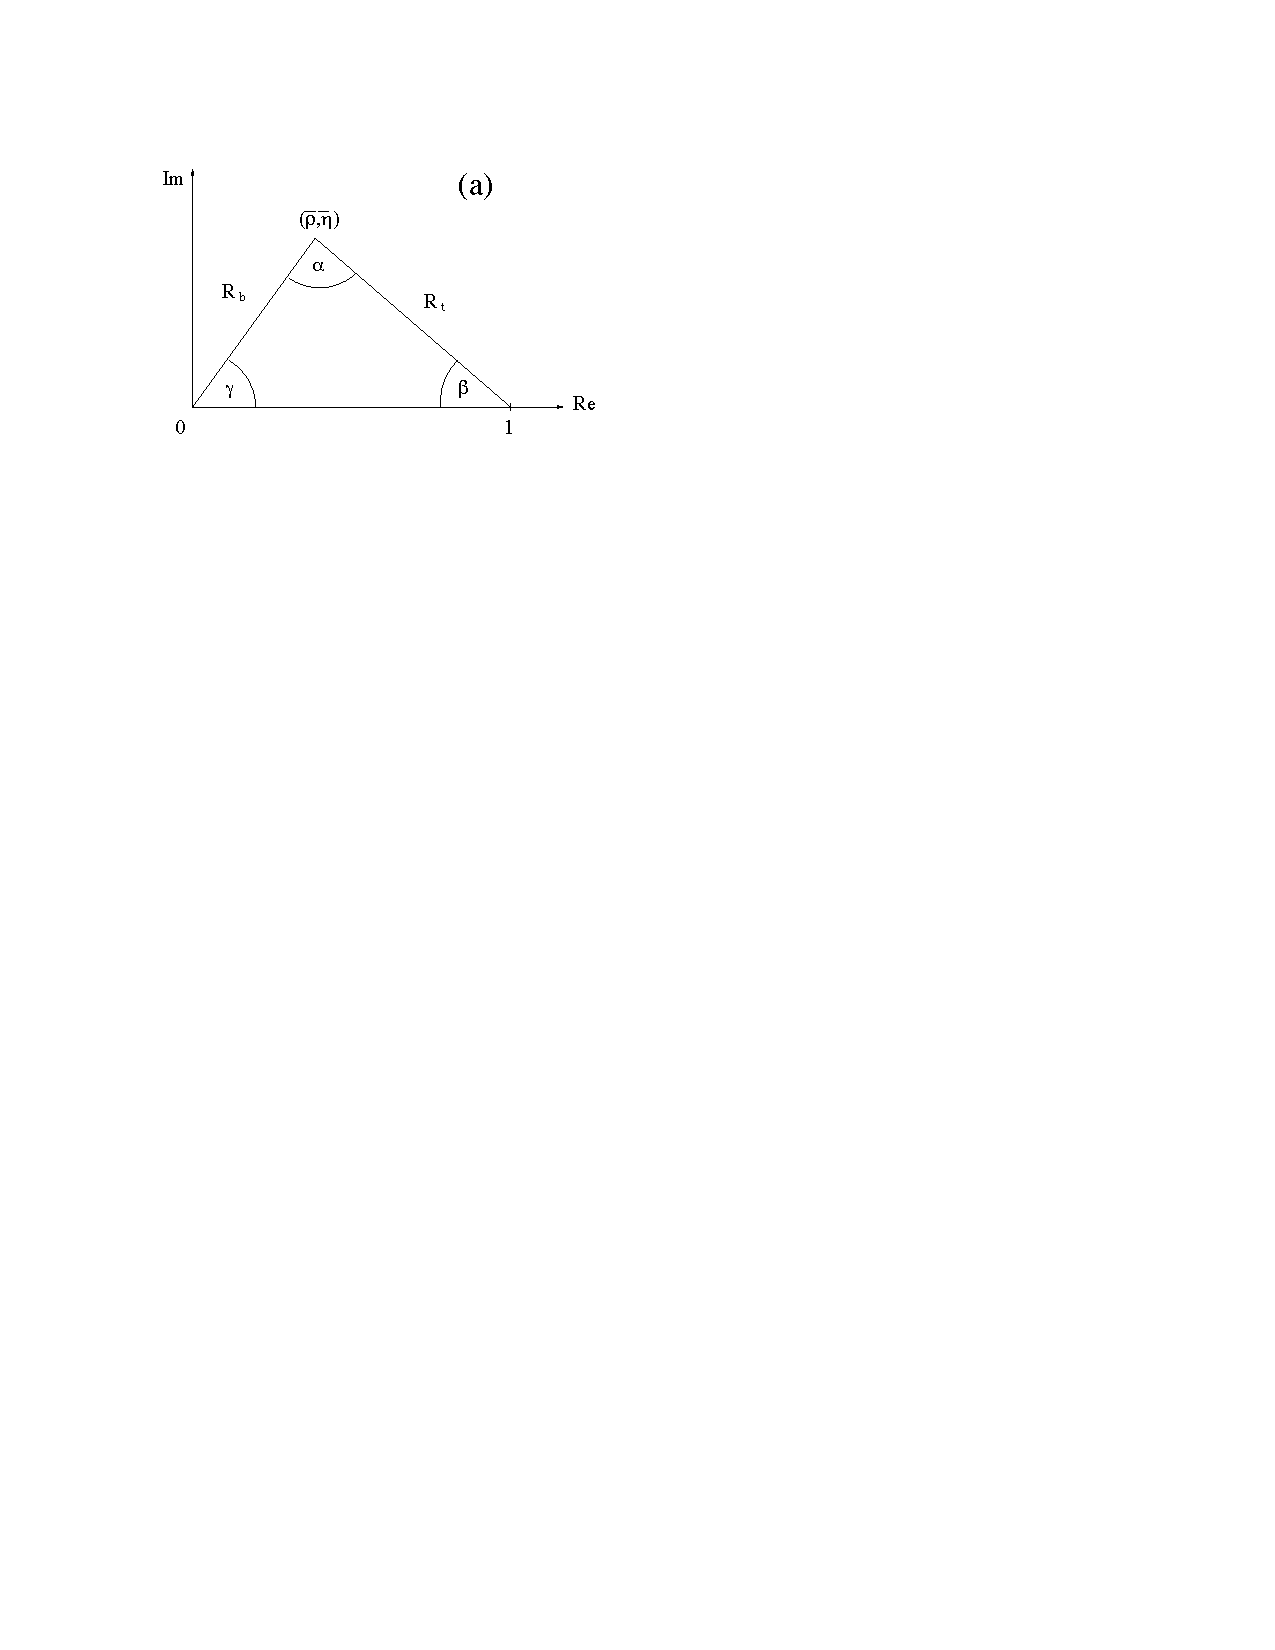
\includegraphics[width=0.5\textwidth]{03-CPViolation/figs/CKMtriangle_prelim.pdf}
\caption{Schematic representation of the CKM unitarity triangle.}
\label{fig:cpviolation:ckmtriangle}
\end{figure}
\todo{replace CKM triangle by self-made version}
Using the parametrisation of the CKM matrix by
Wolfenstein~\cite{Wolfenstein:1983yz}, which is an expansion in powers of
$\lambda \equiv |\Vus| = \num{0.2248\pm0.0006}$~\cite{PDG2016}
\begin{align}
\matr{V}_{\text{CKM}} =
\begin{pmatrix}
1 - \frac 12 \lambda^2 & \lambda & A\lambda^3(\rho - i\eta) \\
- \lambda & 1 - \frac 12 \lambda^2 & A\lambda^2 \\
A\lambda^3(1 - \rho - i\eta) & -A\lambda^2 & 1
\end{pmatrix}
+ \mathcal{O}(\lambda^4)
\end{align}
the other two sides are given by
\begin{align}
	R_b &= \left(1 - \frac{\lambda^2}2\right)\frac 1\lambda \left|\frac \Vub\Vcb\right| = \sqrt{\bar{\rho}^2 + \bar{\eta}^2}\,,\label{eq:cpviolation:Rb}\\
	R_t &= \frac 1\lambda \left|\frac \Vtd\Vcb\right| = \sqrt{(1 - \bar{\rho})^2 + \bar{\eta}^2}\,,
\end{align}
where $\bar{\rho}$ and $\bar{\eta}$ define the position of the apex and are
related to the Wolfenstein parameters through
\begin{align}
	\bar{\rho} = \rho(1 - \lambda^2/2)\quad \text{and} \quad \bar{\eta} = \eta(1 - \lambda^2/2)\,.
\end{align}
The three angles of the unitarity triangle are defined by
\begin{align}
	\alpha \equiv \text{arg}\left(-\frac{\Vtd\Vtbs}{\Vud\Vubs}\right)\,,\quad
	\beta \equiv \text{arg}\left(-\frac{\Vcd\Vcbs}{\Vtd\Vtbs}\right)\,,\quad
	\gamma \equiv \text{arg}\left(-\frac{\Vud\Vubs}{\Vcd\Vcbs}\right)\,.
\label{eq:cpviolation:angles}
\end{align}

The unitarity triangle is overconstrained, \ie there are measurements of more
independent parameters than necessary to fully characterise the shape of the
triangle. The angle $\alpha$ can be studied with \BdToPiPi
decays~\cite{BaBar_alpha,Belle_alpha,LHCb-PAPER-2013-040}, $\beta$ is
precisely measured using the time-dependent \CP asymmetry in \BdToJPsiKS
decays (see \cref{sec:cpviolation:btoccbars}), and $\gamma$ can be extracted
from a combination of results in \BToDh decays~\cite{LHCb-CONF-2016-001}.
Semileptonic $b$-hadron decays are used to determine the size of the triangle
side $R_b$. Further information on $|\Vub|$ comes from studies of \BuToTauNu
decays~\cite{BaBar_BToTauNu,Belle_BToTauNu_HT,Belle_BToTauNu_SL}. The second
non-trivial side length $R_t$ is constrained by measurements of the mixing
frequencies \dmd and \dms in the system of neutral \Bd and \Bs
mesons~\cite{HFAG}. Furthermore, information on the position of the apex can
be gained from the measurement of \CP violation in the neutral kaon
system~\cite{PDG2016}. All these inputs are put into a global fit, which
mainly checks how well the different constraints agree on the position of the
apex. The latest result of the CKMfitter group in
\cref{fig:cpviolation:ckmtriangle_fitted} shows a very good agreement of all
present tests of \CP violation in the SM as the area for the position of the
apex is relatively small.
\begin{figure}
\centering
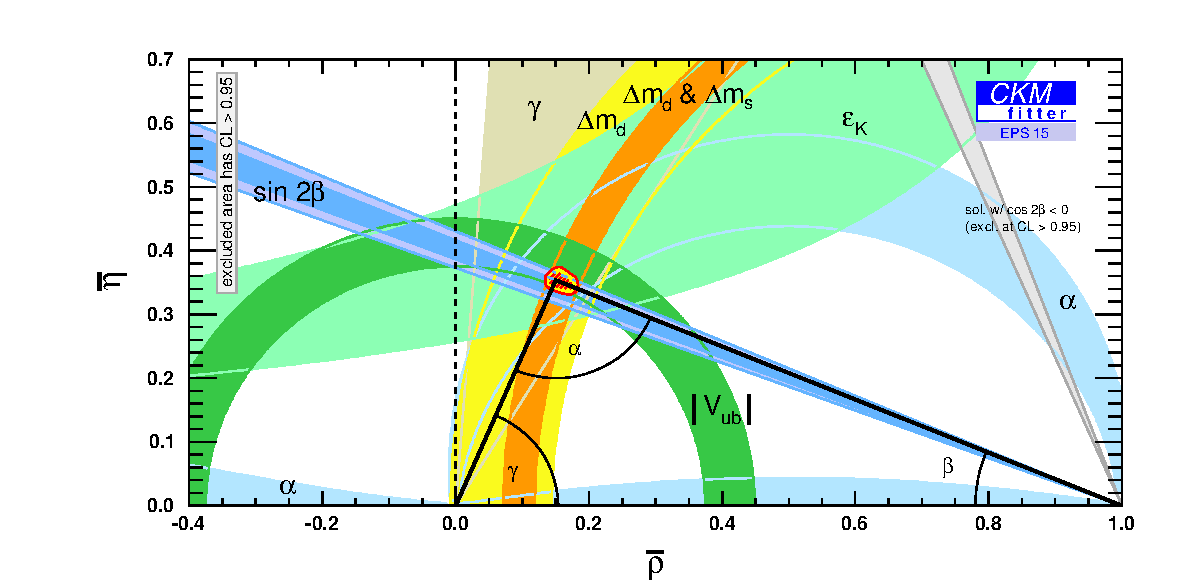
\includegraphics[width=\textwidth]{03-CPViolation/figs/CKMfitterTriangle.pdf}
\caption{Unitarity triangle with constraints from measurements of various
quantities~\cite{CKMfitter}.}
\label{fig:cpviolation:ckmtriangle_fitted}
\end{figure}


%!TEX root = ../main.tex

\section{The system of neutral \texorpdfstring{$\Bd$}{B0} mesons (3 pages)}
\label{sec:cpviolation:neutralBmesons}

%!TEX root = ../main.tex

\section{Types of \texorpdfstring{$\CP$}{CP} violation}
\label{sec:cpviolation:types}

There are three different manifestations of \CP violation. It can occur, when
the decay amplitudes differ between \CP conjugated processes (see
\cref{sec:cpviolation:types:direct}), when the mass eigenstates are no \CP
eigenstates (see \cref{sec:cpviolation:types:indirect}), and when there is
interference between direct decays and decays to the same final state after
mixing (see \cref{sec:cpviolation:types:interference}). While the first type
can appear for charged and neutral hadrons, the latter are only possible for
neutral decays.

All types of \CP violation can be summarized with the condition $\lambda_f
\neq 1$.

%!TEX root = ../main.tex

\subsection{Direct \texorpdfstring{$\CP$}{CP} violation}
\label{sec:cpviolation:types:direct}

Two different type of phases can contribute to decay amplitudes, weak phases
and strong phases. Weak phases can enter through the CKM matrix and take the
opposite sign for \Af and \Abarfbar. Strong phases typically appear in
scattering processes and originate from intermediate on-shell states. They
occur with the same sign in \Af and \Abarfbar. However, only phase differences
are physically meaningful, as the SM is a gauge-invariant theory and thus
absolute phases could be removed by a rotation of the system. So, at least two
terms with different weak and strong phases need to contribute to the decay
amplitudes to have an effect. The superposition of several contributions with
individual magnitudes $A_i$, weak phases $e^{i\phi_i}$ and strong phases
$e^{i\delta_i}$ leads to
\begin{align}
\begin{split}
	\Af = &\sum_i A_i e^{i(\delta_i+\phi_i)}\,,\\
	\Abarfbar = e^{2i(\xi_f-\xi_B)}&\sum_i A_i e^{i(\delta_i-\phi_i)}\,,
\end{split}
\end{align}
where $\xi_f$ and $\xi_B$ are arbitrary phases coming from the \CP
transformation on the \Bd meson and the final state, respectively. If the
final state $f$ is a \CP eigenstate, the term $e^{2i\xi_f} = \num{\pm1}$
represents the \CP eigenvalue. Direct \CP violation is present for
\begin{align}
	\left|\frac{\Abarfbar}{\Af}\right| = \left|\frac{\sum A_i e^{i(\delta_i-\phi_i)}}{\sum A_i e^{i(\delta_i+\phi_i)}}\right| \neq 1\,.
\end{align}

This type of \CP violation is observed in charmless two-body decays of neutral
$B$ mesons~\cite{Lees:2012mma,Duh:2012ie,LHCb-PAPER-2013-018}.

%!TEX root = ../main.tex

\subsection{Indirect \texorpdfstring{$\CP$}{CP} violation}
\label{sec:cpviolation:types:indirect}

Indirect \CP violation occurs when the mass eigenstates are no \CP eigenstates
and instead a relative phase is present between $M_{12}$ and $\Gamma_{12}$.
Following \cref{eq:cpviolation:neutralBmesons:qp} this means
\begin{align}
	\left|\frac qp \right| \neq 1\,.
\end{align}
So, it can be interpreted as difference of the mixing probabilities between
\Bd and \Bdb mesons
\begin{align}
	\mathcal{P}(\Bd\!\to\Bdb,t) \neq \mathcal{P}(\Bdb\!\to\Bd,t)\,,
\end{align}
and thus is also called \CP violation in mixing. While this type of \CP
violation has been observed in the system of neutral kaons, all measurements
in the system of neutral $B$ mesons yield values for the asymmetry of
semileptonic decays
\begin{align}
	a_{\mathrm{sl}} = \frac{\Gamma(\Bdb(t)\!\to\ellp\nu X) - \Gamma(\Bd(t)\!\to\ellm\nu X)}{\Gamma(\Bdb(t)\!\to\ellp\nu X) + \Gamma(\Bd(t)\!\to\ellm\nu X)} = \frac{1 - |q/p|^4}{1 + |q/p|^4}
\end{align}
consistent with zero~\cite{LHCb-PAPER-2014-053,LHCb-PAPER-2016-013}, though
the precision is one to two magnitudes above the SM expectations. This lack in
precision is not only due to statistical uncertainties. When extracting the
\CP asymmetry from the raw asymmetry further asymmetries, like detection and
production asymmetries, need to be taken into account, and these are not
precisely known.

%!TEX root = ../main.tex

\subsection{\texorpdfstring{$\CP$}{CP} violation in the interference of decay and decay after mixing (2 pages)}
\label{sec:cpviolation:types:interference}

%!TEX root = ../main.tex

\section{\texorpdfstring{$\CP$}{CP} violation in \texorpdfstring{$\bToccbars$}{bToccbars} decays (2 pages)}
\label{sec:cpviolation:btoccbars}

The gold-plated mode to measure \CP violation in the system of neutral $B$
mesons is \BdToJPsiKS. It proceeds via a \bToccbars transition. Direct and
indirect \CP violation is strongly suppressed, which makes it a very clean
mode to determine the weak mixing phase, and thus the CKM angle $\beta$, via
\CP violation in the interference of decay and decay after mixing. As the
Feynman diagrams in \cref{fig:cpviolation:bd2jpsiks_feynmans} show, actually
\BdToJPsiKz and \BdbToJPsiKzb decays take place.
\begin{figure}[htb]
\centering
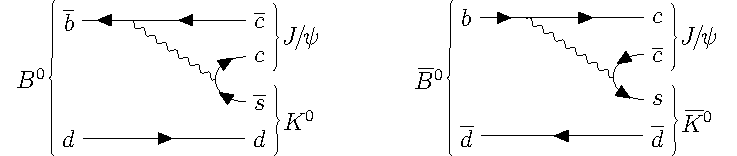
\includegraphics[width=\textwidth]{03-CPViolation/tikz/pdf/BdToJPsiKS_Feynmans.pdf}
\caption{Tree Feynman diagrams of \BdToJPsiKS for both flavours.}
\label{fig:cpviolation:bd2jpsiks_feynmans}
\end{figure}
However, like for the $B$ mesons the flavour eigenstates are a superposition
of the \CP mass eigenstates:
\begin{align}
	\ket{\KS} = p_K \ket{\Kz} - q_K \ket{\Kzb}
\end{align}
Therefore, the ratio of decay amplitudes is composed of two terms according to
\begin{align}
	\frac{\bar{A}_{\JPsi\KS}}{A_{\JPsi\KS}} = -\frac{p_K}{q_K}\frac{\bar{A}_{\JPsi\Kzb}}{A_{\JPsi\Kz}}\,.
\end{align}
The ratio of the mixing coefficients for the kaons can be calculated using
\cref{eq:cpviolation:qp}. Different than for the $B$ mesons the dominant
contribution to the mixing diagrams arises from charm quarks in the loop:
\begin{align}
	\frac{p_K}{q_K} = -\frac{\Vcs\Vcds}{\Vcss\Vcd}
\end{align}
Accounting only for the tree diagrams in
\cref{fig:cpviolation:bd2jpsiks_feynmans}, while neglecting loop processes,
the ratio of the direct decay amplitudes can be expressed via the involved CKM
matrix elements:
\begin{align}
	\frac{\bar{A}_{\JPsi\Kzb}}{A_{\JPsi\Kz}} = \frac{\Vcb\Vcss}{\Vcbs\Vcs}
\end{align}
Summarising these values and adding the ratio of CKM matrix elements for the
mixing of the \Bd mesons (see \cref{eq:cpviolation:qp_simplified}) the
parameter describing \CP violation from \cref{eq:cpviolation:lambda} becomes
\begin{align}
	\lambda_{\JPsi\KS} = - \frac{\Vtbs\Vtd}{\Vtb\Vtds}\frac{\Vcs\Vcds}{\Vcss\Vcd}\frac{\Vcb\Vcss}{\Vcbs\Vcs} = - \frac{\Vtbs\Vtd}{\Vtb\Vtds}\frac{\Vcds\Vcb}{\Vcd\Vcbs}
\end{align}
The minus sign indicates that the final state $\JPsi\KS$ is \CP-odd, as an
angular momentum of $l = 1$ is necessary to compensate that the \Bd meson as
initial state has spin zero, while the final state consists of a \CP-even
$\JPsi$ meson with spin one and an almost \CP-even\footnote{When reconstructed
in a pair of two pions it is fully \CP-even.} \KS meson with spin zero.

%!TEX root = ../main.tex

\section{\texorpdfstring{$\CP$}{CP} violation in \texorpdfstring{$\bToccbard$}{bToccbard} decays}
\label{sec:cpviolation:btoccbard}

The decay \BdToDD can be described with the Feynman diagrams in
\cref{fig:cpviolation:feynmandiagrams_bdtodd}.
\begin{figure}[htb]
\centering
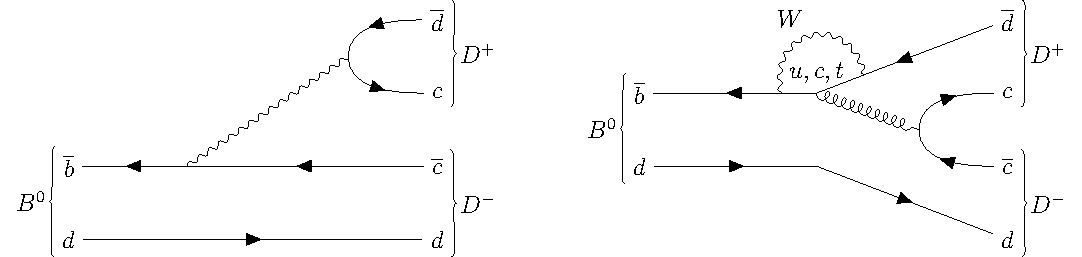
\includegraphics[width=\textwidth]{03-CPViolation/tikz/pdf/BdToDD_Feynmans.pdf}
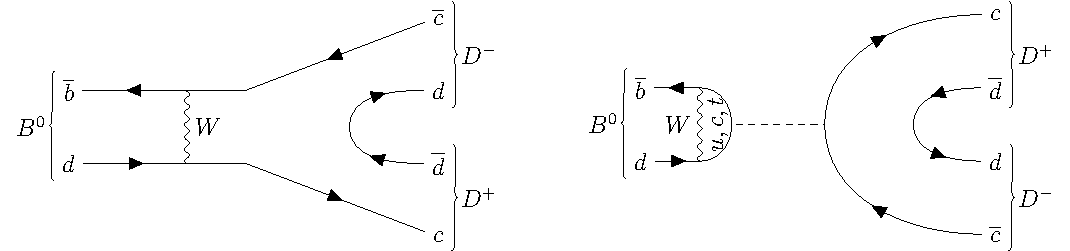
\includegraphics[width=\textwidth]{03-CPViolation/tikz/pdf/BdToDD_Feynmans2.pdf}
\caption{Main Feynman diagrams contributing to \BdToDD decays. Apart from the
tree diagram (top left), a penguin diagram (top right), an exchange diagram
(bottom left) and a penguin annihilation diagram (bottom right) are shown.}
\label{fig:cpviolation:feynmandiagrams_bdtodd}
\end{figure}
\todo{improve quality of Feynman diagrams}
The tree diagram ($T$) proceeds via a \bToccbard quark transition, which is
CKM suppressed. The contributions from the other diagrams, especially the
penguin diagrams ($P^{(q)}$ with $q = \cquark$ and \tquark quarks in the
loop), but also exchange ($E$) and penguin annihilation diagrams
($P\!A^{(q)}$), need to be taken into account as well because they can carry
different weak phases and are not Cabibbo-suppressed. Thus, the decay
amplitude is given by~\cite{Fleischer1999,Fleischer2007,Bel:2015wha}
\begin{align}
	A(\BdToDD) = \Vcb \mathcal{A}[1 - ae^{i\theta}e^{i\gamma}]\,,
\end{align}
with
\begin{align}
	\mathcal{A} \equiv \Vcds[T + E + {P^{(c)} + P\!A^{(c)}} - {P^{(t)} + P\!A^{(t)}}]\,,
\end{align}
and
\begin{align}
	ae^{i\theta} \equiv R_b\left[\frac{{P^{(u)} + P\!A^{(u)}} - {P^{(t)} + P\!A^{(t)}}}{T + E + {{P^{(c)} + P\!A^{(c)}} - {P^{(t)} + P\!A^{(t)}}}}\right]\,.
\end{align}
Here, $R_b$ is a side length of the unitarity triangle defined in
\cref{eq:cpviolation:Rb}. The angle $\gamma$ of the unitarity triangle is a
\CP-violating weak phase, while $a$ and $\theta$ are hadronic \CP-conserving
parameters. Therefore, the corresponding \Bzb decay amplitude is
\begin{align}
	A(\BdbToDD) = \Vcbs \mathcal{A}[1 - ae^{i\theta}e^{-i\gamma}]\,.
\end{align}
The parameter describing \CP violation in the interference can be written as
\begin{align}
\begin{split}
	\lambda_{\Dp\Dm} &= \frac{\Vtbs\Vtd}{\Vtb\Vtds}\frac{\Vcb\Vcds}{\Vcbs\Vcd}\frac{1-ae^{i\theta}e^{i\gamma}}{1-ae^{i\theta}e^{-i\gamma}}\,,\\
					 &= e^{-i2\beta}\frac{1-ae^{i\theta}e^{i\gamma}}{1-ae^{i\theta}e^{-i\gamma}}\,,
\end{split}
\end{align}
using the ratio of the mixing coefficients from
\cref{eq:cpviolation:qp_simplified} and the definition of the unitarity
triangle $\beta$ from \cref{eq:cpviolation:angles}. Different than for
\BdToJPsiKS (cf.~\cref{eq:lambda_JPsiKS}) the \CP eigenvalue is $\eta_{\CP} =
\num{+1}$, since no spins are involved in the decay \BdToDD. The hadronic
parameters cannot be calculated reliably within QCD~\cite{Bel:2015wha}. Thus,
they must be determined through a measurement of the \CP observables, which
can be expressed via
\begin{align}
	\SDD &= -\frac{\sin\phid - 2a \cos\theta\sin(\phid + \gamma) + a^2\sin(\phid + 2\gamma)}{1 - 2a\cos\theta\cos\gamma + a^2}\,,\\
	\CDD &= \frac{2a\sin\theta\sin\gamma}{1 - 2a\cos\theta\cos\gamma + a^2}\,.
\end{align}
The term \SDD gives access to the mixing phase \phid, which is related to $\beta$ through
\begin{align}
	\phid = 2\beta + \phi_d^{\mathrm{NP}}\,,
\end{align}
and thus considers new physics contributions as well. While \SDD is caused by
interference between the direct decay and the decay after mixing, \CDD
might differ from zero due to interferences between tree and penguin
contributions. Different than in the case of \BdToJPsiKS only an effective
phase
\begin{align}
	\phideff = \phid + \Delta\phid
\end{align}
with
\begin{align}
	\sin\phideff = -\frac{\SDD}{\sqrt{1 - \CDD^2}}
\end{align}
can be measured in \BdToDD. The phase shift $\Delta\phi$ is given by
\begin{align}
	\tan\Delta\phi = \frac{a^2\sin2\gamma - 2a\cos\theta\sin\gamma}{1 - 2a\cos\rho\cos\gamma + a^2\cos2\gamma}\,.
\end{align}

The decay channel \BsToDsDs is also governed by a \bToccbard transition. It
gives access to \phis. However, the measurement is as well polluted by
hadronic penguin effects. Since \BsToDsDs is related to \BdToDD via U-spin
symmetry, the phase shift $\Delta\phi$ can be transferred.

Further decay modes from the family of \BToDDbar decays are \BdToDstD and
\BdToDstDst, which also enable a determination of \phideff, but introduce
further complications. For \BdToDstD the final state is no \CP eigenstate as
it can be distinguished by the charge of the \Dstarpm meson. Thus, four \CP
observables are needed to describe \CP violation. Furthermore, from an
experimentalist's point of view the final state is not symmetrical in terms of
the charges of pions and kaons and thus a detection asymmetry has to be taken
into account. In the measurement of \CP violation using \BdToDstDst decays,
like for \BsToJPsiPhi decays, an angular-dependent analysis is required.


%!TEX root = ../main.tex

\chapter{Detector and simulation}
\label{sec:Detector}
The paragraph below can be used for the detector
description. Modifications may be required in specific papers to fit
within page limits, to enhance particular detector elements or to
introduce acronyms used later in the text. For journals where strict
word counts are applied (for example, PRL), and space is at a premium,
it may be sufficient to write, as a minimum: ``The LHCb detector is a 
single-arm forward spectrometer covering the pseudorapidity range 
$2 < \eta < 5$, 
described in detail in Refs.~\cite{Alves:2008zz,LHCb-DP-2014-002}''. 
A slightly longer version could specify the most relevant sub-detectors, {\it e.g} 
``The LHCb 
detector~\cite{Alves:2008zz,LHCb-DP-2014-002} is a
single-arm forward spectrometer covering the pseudorapidity range $2 < \eta < 5$, designed for
the study of particles containing b or c quarks. The detector elements that are particularly
relevant to this analysis are: a silicon-strip vertex detector surrounding the pp interaction
region that allows c- and b-hadrons to be identified from their characteristically long
flight distance; a tracking system that provides a measurement of momentum, $p$, of charged
particles; and two ring-imaging Cherenkov detectors that are able to discriminate between
different species of charged hadrons.'' 

\begin{verbatim}
In the following paragraph, references to the individual detector 
performance papers are marked with a * and should only be included 
if the analysis relies on numbers or methods described in the specific 
papers. Otherwise, a reference to the overall detector performance 
paper~\cite{LHCb-DP-2014-002} will suffice. Note also that the text 
defines the acronyms for primary vertex, PV, and impact parameter, IP. 
Remove either of those in case it is not used later on.
\end{verbatim}

The \lhcb detector~\cite{Alves:2008zz,LHCb-DP-2014-002} is a single-arm forward
spectrometer covering the \mbox{pseudorapidity} range $2<\eta <5$,
designed for the study of particles containing \bquark or \cquark
quarks. The detector includes a high-precision tracking system
consisting of a silicon-strip vertex detector surrounding the $pp$
interaction region~\cite{LHCb-DP-2014-001}\verb!*!, a large-area silicon-strip detector located
upstream of a dipole magnet with a bending power of about
$4{\mathrm{\,Tm}}$, and three stations of silicon-strip detectors and straw
drift tubes~\cite{LHCb-DP-2013-003}\verb!*! placed downstream of the magnet.
The tracking system provides a measurement of momentum, \ptot, of charged particles with
a relative uncertainty that varies from 0.5\% at low momentum to 1.0\% at 200\gevc.
The minimum distance of a track to a primary vertex (PV), the impact parameter (IP), 
is measured with a resolution of $(15+29/\pt)\mum$,
where \pt is the component of the momentum transverse to the beam, in\,\gevc.
Different types of charged hadrons are distinguished using information
from two ring-imaging Cherenkov detectors~\cite{LHCb-DP-2012-003}\verb!*!. 
Photons, electrons and hadrons are identified by a calorimeter system consisting of
scintillating-pad and preshower detectors, an electromagnetic
calorimeter and a hadronic calorimeter. Muons are identified by a
system composed of alternating layers of iron and multiwire
proportional chambers~\cite{LHCb-DP-2012-002}\verb!*!.
The online event selection is performed by a trigger~\cite{LHCb-DP-2012-004}\verb!*!, 
which consists of a hardware stage, based on information from the calorimeter and muon
systems, followed by a software stage, which applies a full event
reconstruction.

A more detailed description of the 'full event reconstruction' could be:
\begin{itemize}
\item The trigger~\cite{LHCb-DP-2012-004}\verb!*! consists of a
hardware stage, based on information from the calorimeter and muon
systems, followed by a software stage, in which all charged particles
with $\pt>500\,(300)\mev$ are reconstructed for 2011\,(2012) data.
For triggers that require neutral particles, 
energy deposits in the electromagnetic calorimeter are 
analysed to reconstruct \piz and $\gamma$ candidates.
\end{itemize}

The trigger description has to be specific for the analysis in
question. In general, you should not attempt to describe the full
trigger system. Below are a few variations that inspiration can be
taken from. First from a hadronic analysis, and second from an
analysis with muons in the final state.
A detailed description of the trigger conditions for Run 1 is available in Ref.~\cite{LHCb-PUB-2014-046}.
\begin{itemize}
\item At the hardware trigger stage, events are required to have a muon with high \pt or a
  hadron, photon or electron with high transverse energy in the calorimeters. For hadrons,
  the transverse energy threshold is 3.5\gev.
  The software trigger requires a two-, three- or four-track
  secondary vertex with a significant displacement from the primary
  $pp$ interaction vertices. At least one charged particle
  must have a transverse momentum $\pt > 1.7\gevc$ and be
  inconsistent with originating from a PV.
  A multivariate algorithm~\cite{BBDT} is used for
  the identification of secondary vertices consistent with the decay
  of a \bquark hadron.
%\item The software trigger requires a two-, three- or four-track
%  secondary vertex with a large sum of the transverse momentum, \pt, of
%  the tracks and a significant displacement from the primary $pp$
%  interaction vertices~(PVs). At least one track should have $\pt >
%  1.7\gevc$ and \chisqip with respect to any
%  primary interaction greater than 16, where \chisqip is defined as the
%  difference in \chisq of a given PV reconstructed with and
%  without the considered track.\footnote{If this sentence is used to define \chisqip
%  for a composite particle instead of for a single track, replace ``track'' by ``particle'' or ``candidate''}
% A multivariate algorithm~\cite{BBDT} is used for
%  the identification of secondary vertices consistent with the decay
%  of a \bquark hadron.
\item Candidate events are first required to pass the hardware trigger,
  which selects muons with a transverse momentum $\pt>1.48\gevc$ 
  in the 7\tev data or $\pt>1.76\gevc$ in the 8\tev data.
  In the subsequent software trigger, at least
  one of the final-state particles is required to have both
  $\pt>0.8\gevc$ and impact parameter larger than $100\mum$ with respect to all
  of the primary $pp$ interaction vertices~(PVs) in the
  event. Finally, the tracks of two or more of the final-state
  particles are required to form a vertex that is significantly
  displaced from the PVs.
\end{itemize}

An example to describe the use of both TOS and TIS events:
\begin{itemize}
\item In the offline selection, trigger signals are associated with reconstructed particles.
%Selection requirements can therefore be made not only on the trigger requirement,
%but on whether the decision was due to the signal candidate, other particles produced in the $pp$ collision, or a combination of both.
Selection requirements can therefore be made on the trigger selection itself
and on whether the decision was due to the signal candidate, other particles produced in the $pp$ collision, or a combination of both.
\end{itemize}

A good example of a description of long and downstream \KS is given in 
Ref.~\cite{LHCb-PAPER-2014-006}:
\begin{itemize}
\item
Decays of \decay{\KS}{\pip\pim} are reconstructed in two different categories:
the first involving \KS mesons that decay early enough for the
daughter pions to be reconstructed in the vertex detector; and the
second containing \KS that decay later such that track segments of the
pions cannot be formed in the vertex detector. These categories are
referred to as \emph{long} and \emph{downstream}, respectively. The
long category has better mass, momentum and vertex resolution than the
downstream category.
\end{itemize}

The description of our software stack for simulation is often
causing trouble. The following paragraph can act as inspiration but
with variations according to the level of detail required and if
mentioning of \eg \photos is required.
\begin{itemize}
\item In the simulation, $pp$ collisions are generated using
\pythia~\cite{Sjostrand:2006za,*Sjostrand:2007gs} 
(In case only \pythia 6 is used, remove \verb=*Sjostrand:2007gs= from this citation; if 
only \pythia 8 is used, then reverse the order of the papers in the citation.)
 with a specific \lhcb
configuration~\cite{LHCb-PROC-2010-056}.  Decays of hadronic particles
are described by \evtgen~\cite{Lange:2001uf}, in which final-state
radiation is generated using \photos~\cite{Golonka:2005pn}. The
interaction of the generated particles with the detector, and its response,
are implemented using the \geant
toolkit~\cite{Allison:2006ve, *Agostinelli:2002hh} as described in
Ref.~\cite{LHCb-PROC-2011-006}.
\end{itemize}

Many analyses depend on boosted decision trees. It is inappropriate to
use TMVA as the reference as that is merely an implementation of the
BDT algorithm. Rather it is suggested to write

In this paper we use a boosted decision tree~(BDT)~\cite{Breiman,AdaBoost} to separate signal from
background.

When describing the integrated luminosity of the data set, do not use
expressions like ``1.0\,fb$^{-1}$ of data'', but \eg 
``data corresponding to an integrated luminosity of 1.0\,fb$^{-1}$'', 
or ``data obtained from 3\,fb$^{-1}$ of integrated luminosity''. 

For analyses where the periodical reversal of the magnetic field is crucial, 
\eg in measurements of direct \CP violation, the following description can be
used as an example phrase: 
``The polarity of the dipole magnet is reversed periodically throughout data-taking.
The configuration with the magnetic field vertically upwards, \MagUp (downwards, \MagDown), bends positively (negatively)
charged particles in the horizontal plane towards the centre of the LHC.''
Only use the \MagUp, \MagDown symbols if they are used extensively in tables or figures.


%!TEX root = ../main.tex

\chapter{Data Analysis Tools and Methods (12 pages)}
\label{sec:dataanalysis}

%!TEX root = ../main.tex

\section{Maximum likelihood method (1 page)}
\label{sec:dataanalysis:maximumlikelihood}

%!TEX root = ../main.tex

\section{Selection (5 pages)}
\label{sec:b02dd:selection}

The amount of background in \BdToDD is too high to perform a significant
measurement of \CP violation without any selection. The selection is divided
into three parts: a preselection with many high signal efficiency
requirements, a dedicated treatment of mis-identified backgrounds and a
multivariate analysis to further reduce combinatorial background.

\subsection{Preselection}
\label{sec:b02dd:selection:cuts}

Only events that have been triggered by a topological trigger line or by the
inclusive $\phi$ line and that in total contain less than \num{500} long
tracks are considered. All candidate kaon and pion tracks have to be long
tracks and have to satisfy quality criteria. Lower limits on the momentum ($p
> \SI{1}{\GeVc}$) and on the transverse momentum ($\pT > \SI{100}{\MeVc}$) are
required. The candidates should be inconsistent with originating from the PV
and the particle identification (PID) system needs to classify them as pions
or kaons with only a small probability to be a ghost.

Of all the possible combinations of three charged hadron tracks forming a
$\Dp$ meson candidate only the two possibilities \DToKpipi and \DToKKpi are
used. The vertex needs to be significantly displaced from all PVs in the event
and the distance of the closest approach between all pairs of particles
forming the vertex has to be below \SI{0.5}{\mm}. The scalar sum of the \pT
has to exceed \SI{1800}{\MeVc} and the combined invariant mass has to be in
the range \SI{\pm25}{\MeVcc} around the nominal \Dp mass~\cite{PDG2014}. The
tightened mass window as well as requiring that the \chisq of the flight
distance of each $\Dpm$ meson with respect to the $\Bd$ decay vertex has to be
larger than \num{2} reduces the amount of (partially) charmless contributions.
On top of that, a cut on the decay time significance of the $\Dpm$ mesons,
defined as their decay time with respect to the $\Bz$ decay vertex divided by
the corresponding uncertainty, is supposed to further suppress the (partially)
charmless contributions. The optimal cut value is estimated under the
assumption that a very tight cut leaves only candidates with resonant $\Dpm$
mesons. Gradually loosening the cut the value can be found where the product
of the \Bd signal yield, extracted from a fit on data, and the signal
efficiency, determined on MC, exceeds the estimation from the initial tight
cut scenario. If both $\Dpm$ mesons are reconstructed via \DToKpipi decays the
decay time significance has to be greater than \num{0}. It needs to be greater
than \num{3} if one of the $\Dpm$ mesons is reconstructed in the \KKpi and the
other in the \Kpipi final state. Although in this case the final states
of the \Dpm mesons differ the same cut is applied to both \Dpm mesons as on
signal MC the comparison of the distributions of the decay time significance
shows a good agreement between \DToKpipi and \DToKKpi decays.

The vertex formed by a pair of oppositely charged $\Dpm$ candidates needs to
be of good quality. The scalar sum of the $\pT$ of the $\Dpm$ mesons must
exceed $\SI{5}{\GeVc}$. In the stripping a BDT to select $\Bd$ candidates is
applied. The BDT is based on the \pT and the flight distance \chisq of the \Bz
as well as on the sum of the \Bz and both \PD vertex \chisq's divided by the
sum of the degrees of freedom of these vertex fits. Moreover, the \Bd
candidates are required to have $p > \SI{10}{\GeVc}$ and to have
$\chisqip<\num{25}$, where $\chisqip$ is defined as the difference in the
vertex fit $\chi^2$ of the associated PV with and without the $B^0$ candidate.

The reconstructed decay time $t$ of the \Bd candidate is determined from a
DTF, in which the \Bd production vertex is constrained to the position of the
associated PV. Only candidates with decay times in the range
\SIrange{0.25}{10.25}{\ps} are kept. The invariant mass $m_{\Dp\Dm}$ of the
$\Bd$ candidate has to be in the range \SIrange{5150}{5500}{\MeVcc}. It is
calculated from a DTF, in which the invariant masses of $\Kpipi$ and $\KKpi$
are additionally constrained to the known $\Dp$ mass. It is required that
these fits have converged. Further outliers are removed by requiring that the
uncertainty on the invariant mass and on the decay time has to be below
\SI{30}{\MeVcc} and \SI{0.2}{\ps}, respectively, and that the absolute value
of the $z$ coordinate of the PV is smaller than \SI{250}{\milli\meter}.

The signal efficiency of the preselection for the final state with two kaons
is $\SI{82}{\percent}$ at a background rejection of $\SI{94}{\percent}$. For
the final state with three kaons the signal efficiency is
$\SI{67.5}{\percent}$ at a background rejection of $\SI{98}{\percent}$.

\subsection{Vetoes}
\label{sec:b02dd:selection:vetoes}

A $K\rightarrow\pi$ mis-ID can lead to background contributions from
$\DspToKKpi$, which predominantly proceeds through $\DsTophipi$. To reduce
these $\Dsp$ contributions the kaon mass hypothesis is assigned to the pion
with the higher transverse momentum of $\DpToKpipi$ candidates. The candidate
is rejected if the invariant mass of the hypothetical kaon pair is compatible
with the $\phi$ mass of $M_{\phi} = \SI{1019.461}{\MeVcc}$~\cite{PDG2014}
within $\pm\SI{10}{\MeVcc}$ or if the invariant mass $m(\Km\Kp\pip)$ is
compatible with the \Dsp mass of $M_{\Dsp} =
\SI{1968.30}{\MeVcc}$~\cite{PDG2014} within $\pm\SI{25}{\MeVcc}$ and the pion
with the higher \pT (the one that the kaon mass hypothesis is assigned to) has
a larger $\texttt{ProbNN}K$ than $\texttt{ProbNN}\pion$ probability. When
assigning the kaon mass hypothesis to the pion with the lower \pT no vetoes
are applied as no resonant structures at the $\phi$ or the $\Dsp$ mass are
found.

To reduce $p\rightarrow\pi$ mis-ID the proton mass hypothesis is assigned to
the pion with the higher \pT of $\DpToKpipi$ candidates. The candidate is
rejected if the invariant mass of the $\kaon\proton\pion$ combination is
compatible with the \Lc mass of $M_{\Lc} =
\SI{2286.46}{\MeVcc}$~\cite{PDG2014} within $\pm\SI{25}{\MeVcc}$ and the
proton probability $\texttt{ProbNN}p$ of the pion with the higher \pT is
larger than $\texttt{ProbNN}\pion$.

\subsection{Multivariate analysis}
\label{sec:b02dd:selection:mva}

\subsubsection*{BDT training}
\label{sec:b02dd:selection:mva:training}

To further suppress combinatorial background a Boosted Decision Tree
(BDT)~\cite{Breiman,Roe} based on the implementation in
TMVA~\cite{Hocker:2007ht} is trained using a signal MC sample and the upper
mass sideband with $m_{\Dp\Dm} > \SI{5500}{\MeVcc}$. The training is performed
on half of these samples while the other half is used to test the BDT
performance. The selection steps described above, are applied before the
training.

Two BDTs separated by the number of kaons in the \Bd final state are trained.
The importance of the \num{21} input variables to the training differs, which
is considered by their order in \cref{tab:b02dd:selection:mva:inputs}.
%
\begin{table}[!htb]
\centering
\caption{List of input variables used in the training of the BDTs.}
\begin{tabular}{ll}
 \toprule
  BDT for \KpipiKpipi                          &  BDT for \KKpiKpipi                           \\
\midrule
  min(\Dpm $\tau$ significance)                &  PID ratio of \Kpm                            \\
  $B$ direction angle                          &  $B$ direction angle                          \\
  $\log($DTF $\chi^2$/ndof$)$                  &  PID ratio of \Kp                             \\
  PID ratio of \Km                             &  $\log($DTF $\chi^2$/ndof$)$                  \\
  PID ratio of \Kp                             &  PID ratio of \Km                             \\
  min \pT of \Kpm                              &  min(\Dpm $\tau$ significance)                \\
  $\log(B$ impact parameter $\chi^2)$          &  $\log($min($h$ Velo $\chi^2$/ndof)$)$        \\
  $\log($min(\pipm Velo $\chi^2$/ndof)$)$      &  \pT of \Kpm                                  \\
  \pT of \pim with lower \pT                   &  $\log($min(\Kpm T-track $\chi^2$/ndof)$)$    \\
  $\log($min(\Kpm T-track $\chi^2$/ndof)$)$    &  $\log(B$ impact parameter $\chi^2)$          \\
  $\log($min(\pipm T-track $\chi^2$/ndof)$)$   &  PID ratio of \pipm with lower \pT            \\
  PID ratio of \pim with higher \pT            &  $\log($min($h$ VELO-T-Match $\chi^2$)$)$     \\
  \pT of \pip with lower \pT                   &  $\log($min(\Kpm Velo $\chi^2$/ndof)$)$       \\
  PID ratio of \pim with lower \pT             &  PID ratio of single \pipm                    \\
  PID ratio of \pip with higher \pT            &  \pT of \pipm with higher \pT                 \\
  \pT of \pip with higher \pT                  &  $\log($min($h$ T-track $\chi^2$/ndof)$)$     \\
  PID ratio of \pip with lower \pT             &  \pT of \pipm with lower \pT                  \\
  $\log($min($\Kpm$ Velo $\chi^2$/ndof)$)$     &  min \pT of \Kp and \Km                       \\
  $\log($min(\pipm VELO-T-Match $\chi^2$)$)$   &  \pT of single \pipm                          \\
  $\log($min($\Kpm$ VELO-T-Match $\chi^2$)$)$  &  $\log($min($\Kpm$ VELO-T-Match $\chi^2$)$)$  \\
  \pT of \pim with higher \pT                  &  PID ratio of \pipm with higher \pT           \\
\bottomrule
\end{tabular}
\label{tab:b02dd:selection:mva:inputs}
\end{table}
%
One of the input variables is the ratio of the kaon over the sum of the kaon and the
pion probabilities:
%
\begin{equation}
\text{PID ratio} = \frac{\texttt{ProbNN}K}{\texttt{ProbNN}K + \texttt{ProbNN}\pion} \, .
\label{eq:b02dd:selection:pidratio}
\end{equation}
%
It turns out that this ratio performs a little bit better than just using the
simple ProbNN variables. Among the other input variables are observables
related to the kinematics of the decay like transverse momenta, decay time
significances and direction angles, qualities of the track segments in the
VELO and the T-stations, and vertex qualities.

Before the training the input variables are transformed to decorrelate and
decompose them into the principal components, which improves the performance of
the BDT. The BDTs are each built out of \num{700} trees. The depth of the trees is
limited to three. At each node at least \SI{3}{\percent} of the training
events have to be present. The variables are scanned at \num{40} points to
find the optimal cut value. For the boosting the AdaBoost
method~\cite{AdaBoost} with a boost factor of $\beta = \num{0.1}$ is deployed.

Overtraining is checked by applying the BDT on both the training and the
testing sample (see \cref{fig:b02dd:selection:mva:overtraining}).
%
\begin{figure}[!htb]
\centering
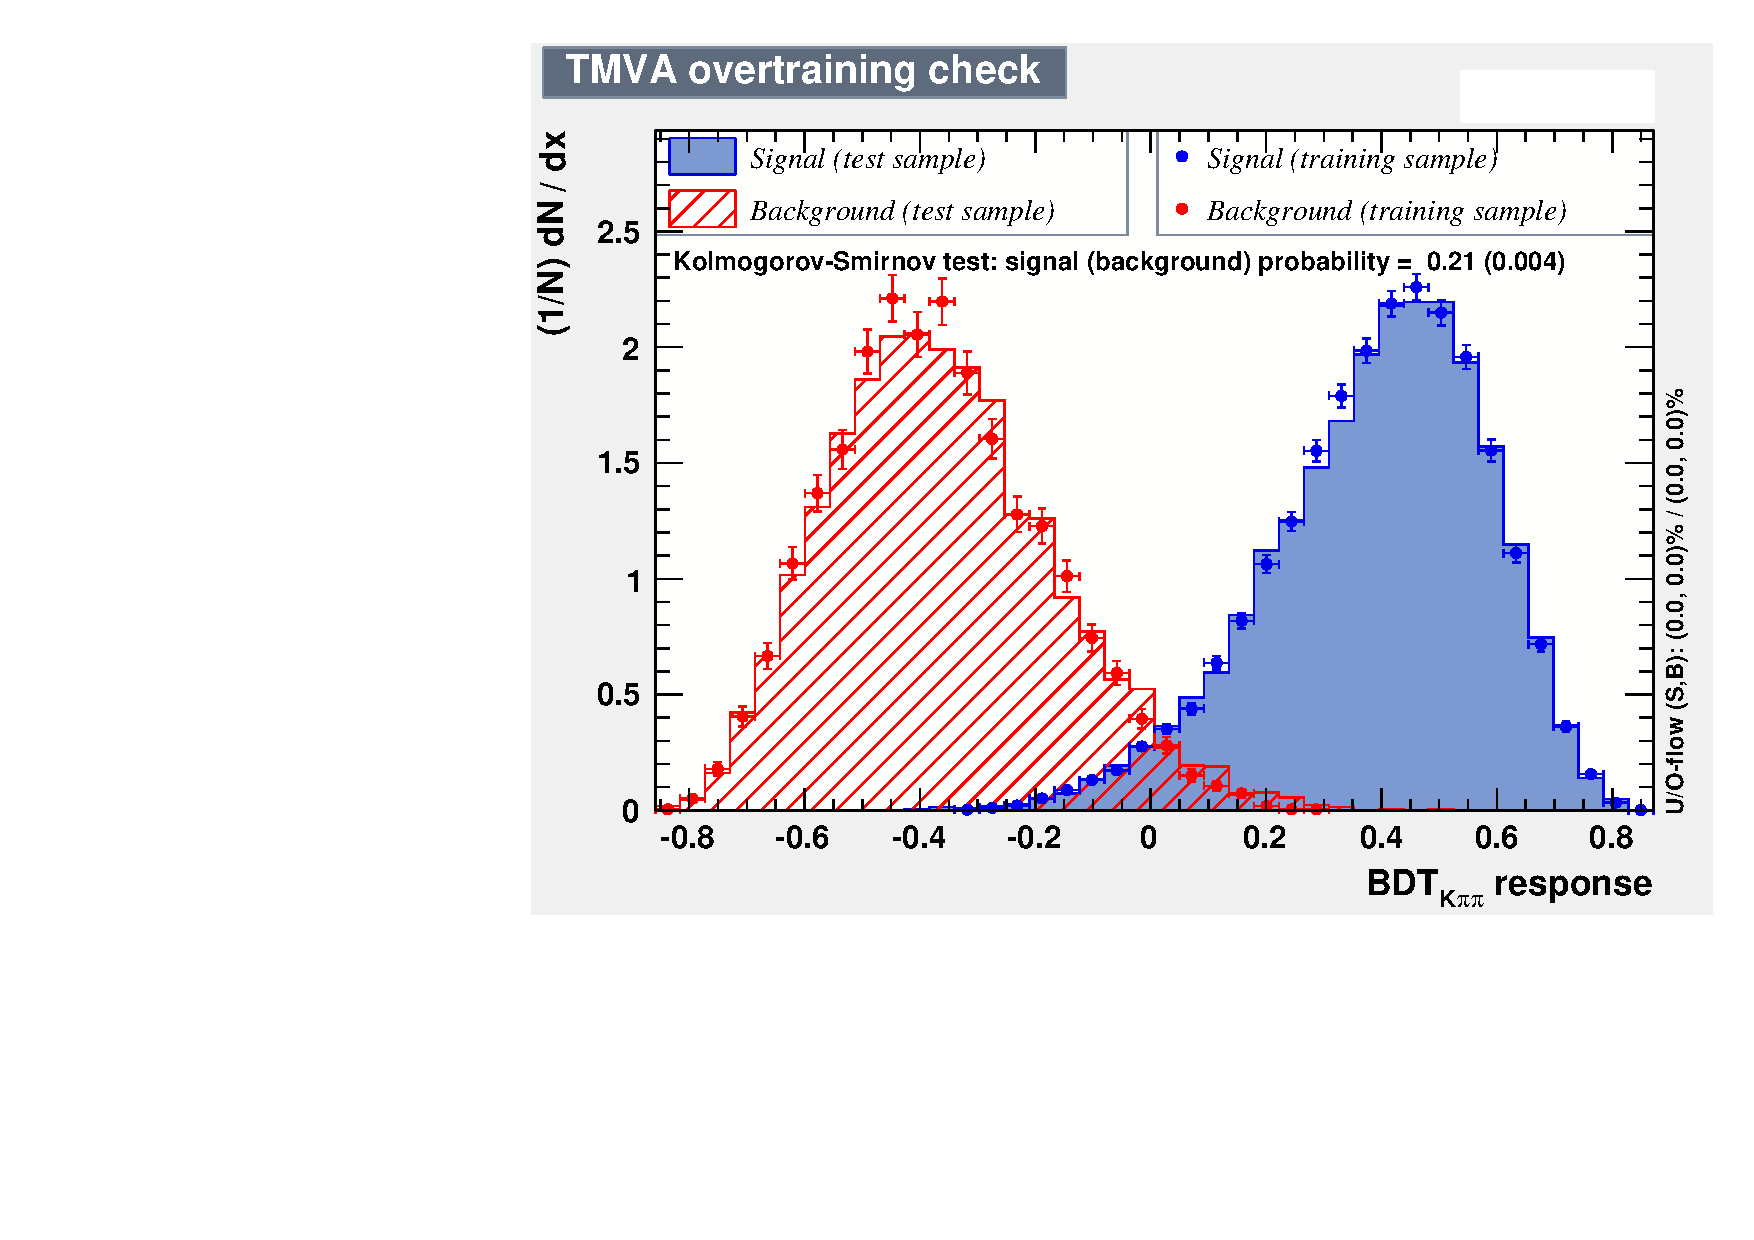
\includegraphics[width=0.48\textwidth]{07-B02DD/figs/Overtraining_Check_Kpipi.pdf}
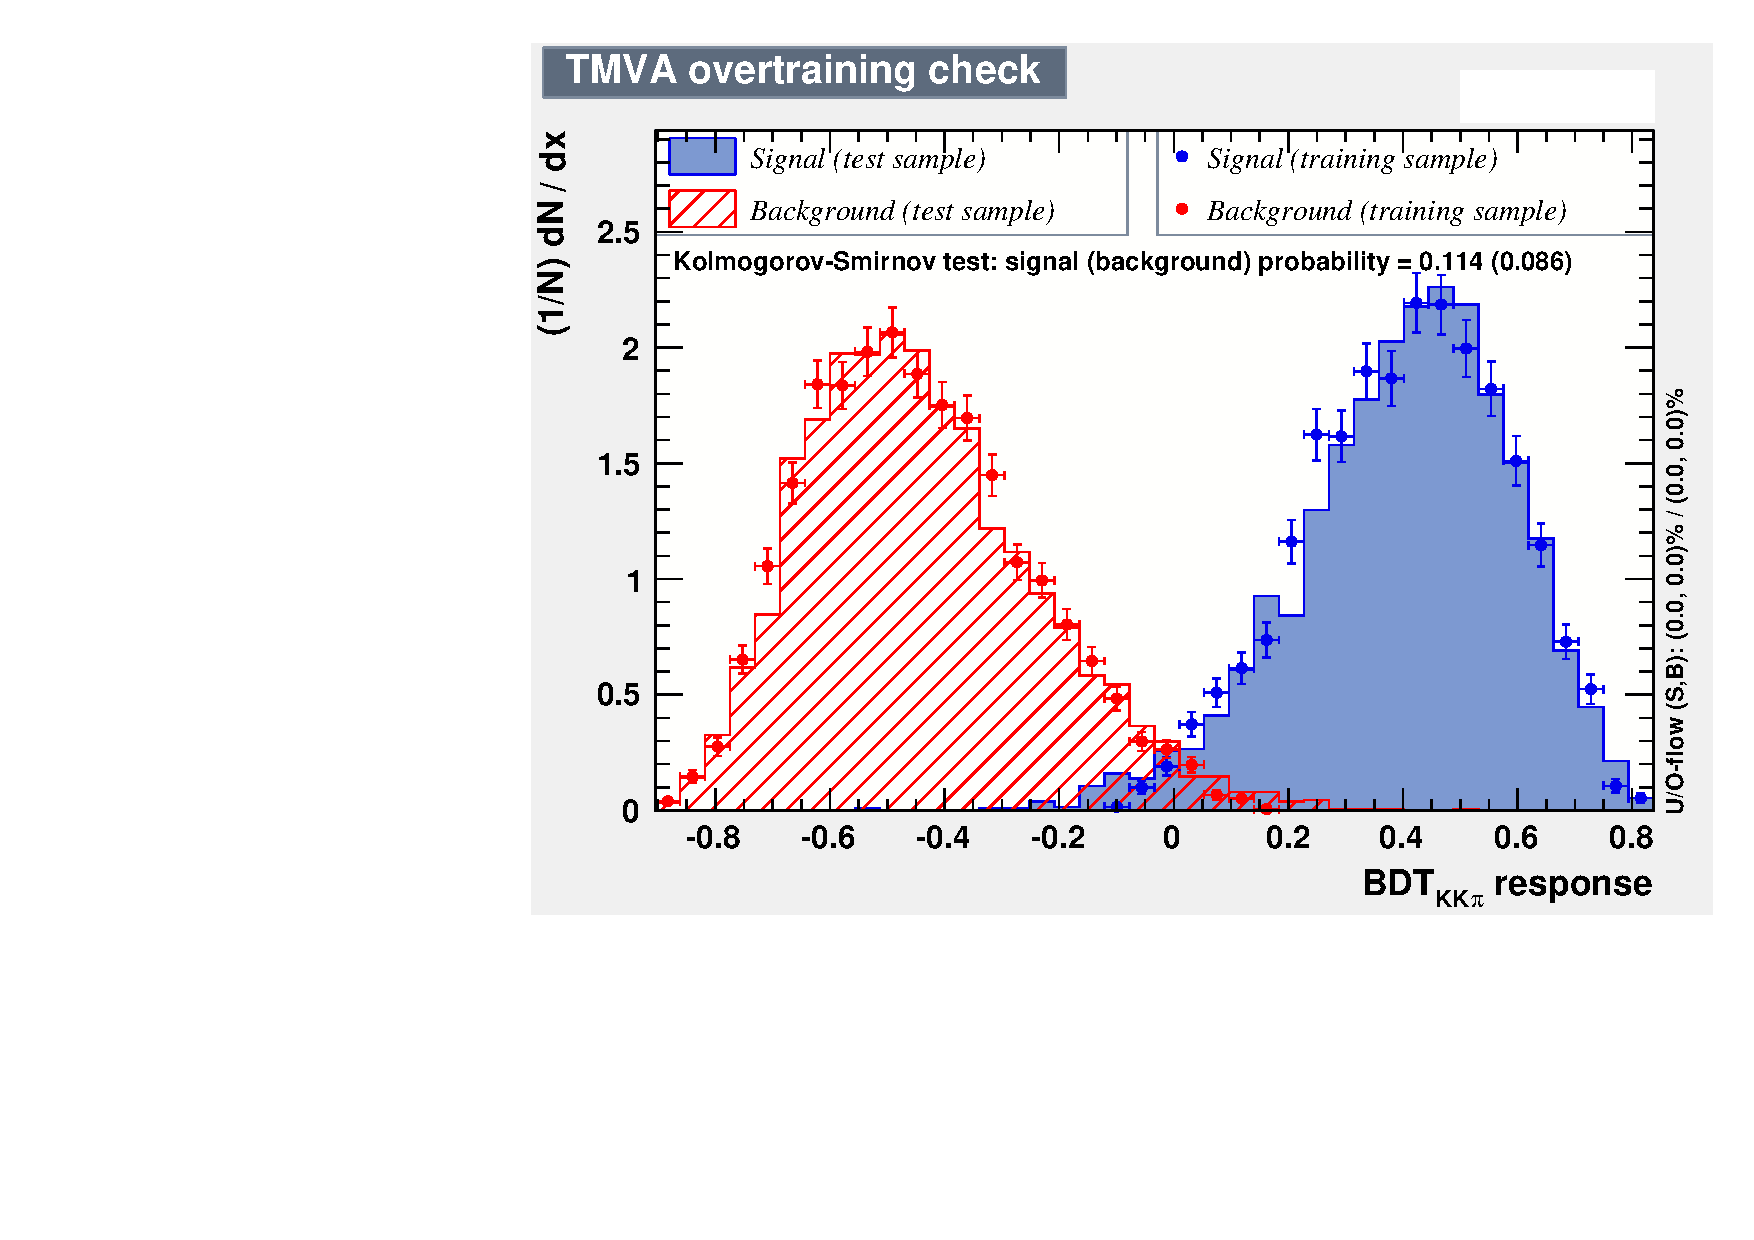
\includegraphics[width=0.48\textwidth]{07-B02DD/figs/Overtraining_Check_KKpi.pdf}
\caption{Comparison of the BDT response on training and test sample for the
\KpipiKpipi final state (left) and the \KKpiKpipi final state (right).}
\label{fig:b02dd:selection:mva:overtraining}
\end{figure}
%
Using simulations in the selection contains the possibility that certain
distributions are not modelled properly and differences between the simulation
and real data are exploited instead of differences between signal and
background. Indeed, the classifier output distributions of the signal MC and
background-subtracted data show a quite large disagreement for both final
states as can be seen in \cref{fig:b02dd:selection:mva:bdtcomparison}. The
performance is clearly overestimated in the training.
%
\begin{figure}[htbp]
    \centering
    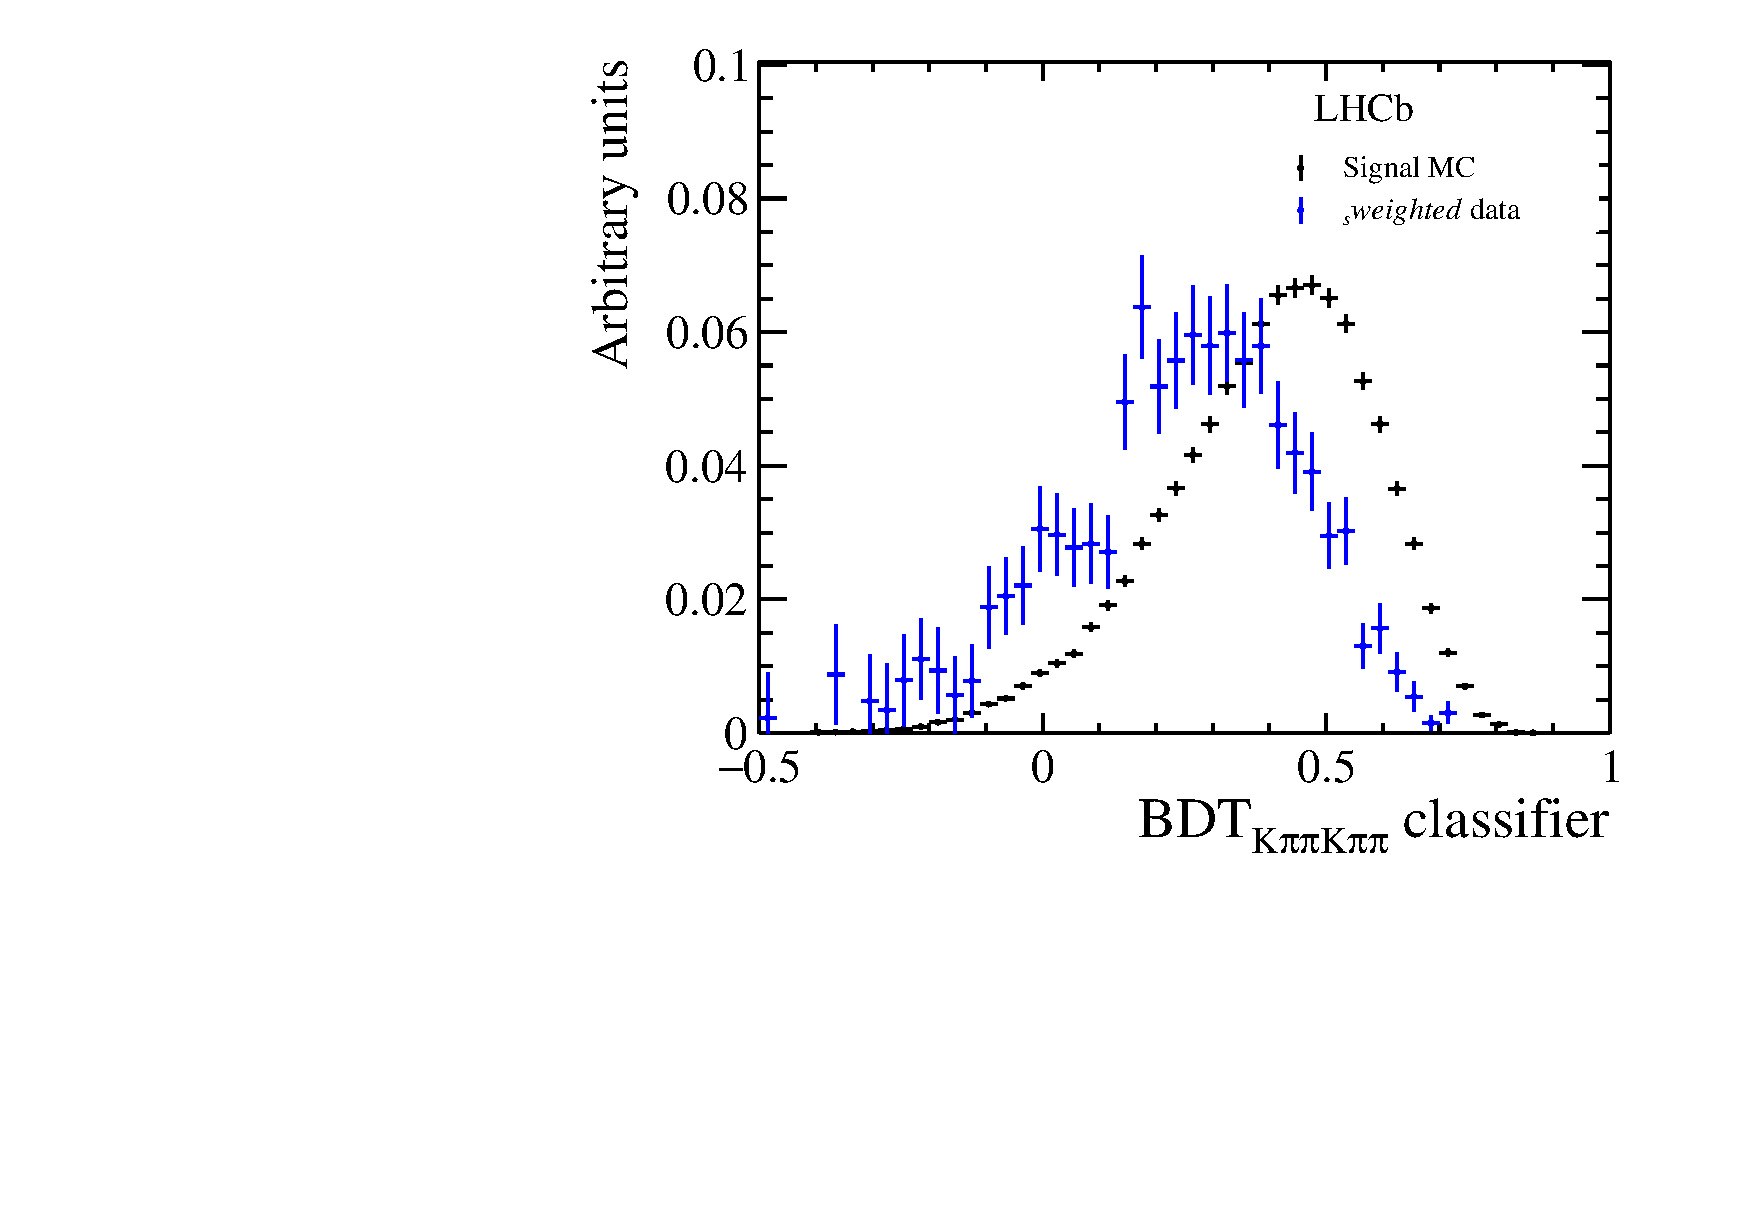
\includegraphics[width=0.49\textwidth]{07-B02DD/figs/BDTComparison_Kpipi.pdf}
    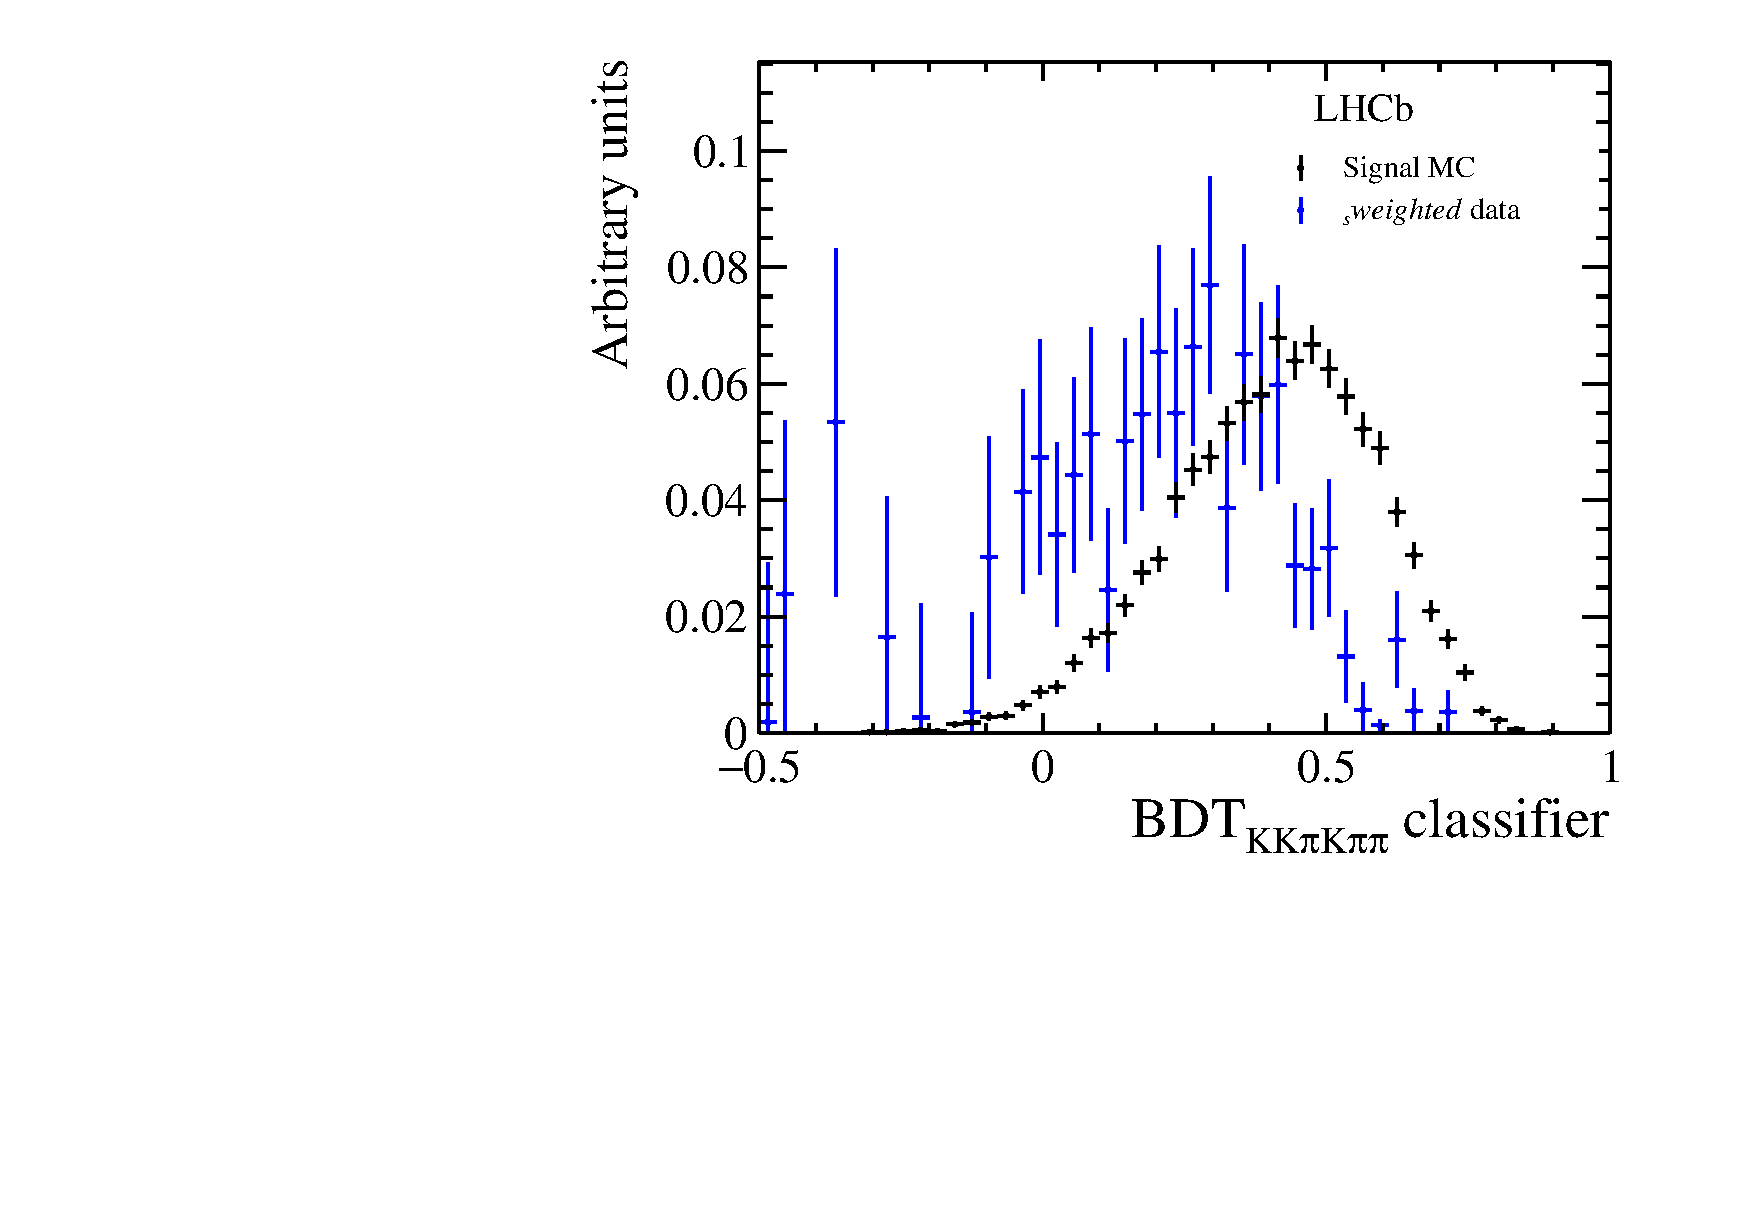
\includegraphics[width=0.49\textwidth]{07-B02DD/figs/BDTComparison_KKpi.pdf}
    \caption{Distribution of the BDT output for background-subtracted data (blue) and
    signal MC (black) for the \KpipiKpipi final state (left) and the
    \KKpiKpipi final state (right).}
    \label{fig:b02dd:selection:mva:bdtcomparison}
\end{figure}
%
This would be a problem if the selection efficiencies had to be calculated
using the MC sample. But for a measurement of \CP violation it is mainly
important that the amount of background can somehow be reduced while most of
the signal is kept. This can be achieved with the current setting.

% ==============================================================================
\subsubsection*{BDT cut optimisation}
\label{sec:b02dd:selection:mva:optimisation}

As explained in \cref{sec:dataanalysis:selection:fom} the best figure of merit
for a measurement of \CP violation is the sensitivity on the \CP observables
themselves. So the requirement on the BDT classifier output is scanned
performing a fit to the invariant $\Dp\Dm$ mass spectrum followed by a decay
time fit of the background-subtracted sample for each scan point. Initially,
only the subsample with two kaons in the \Bd final state is analysed. In
\cref{fig:b02dd:selection:mva:sensitivities} the statistical
uncertainties of \SDD and \CDD are plotted as a function of the requirement on
the BDT classifier output.
%
\begin{figure}[!htb]
\centering
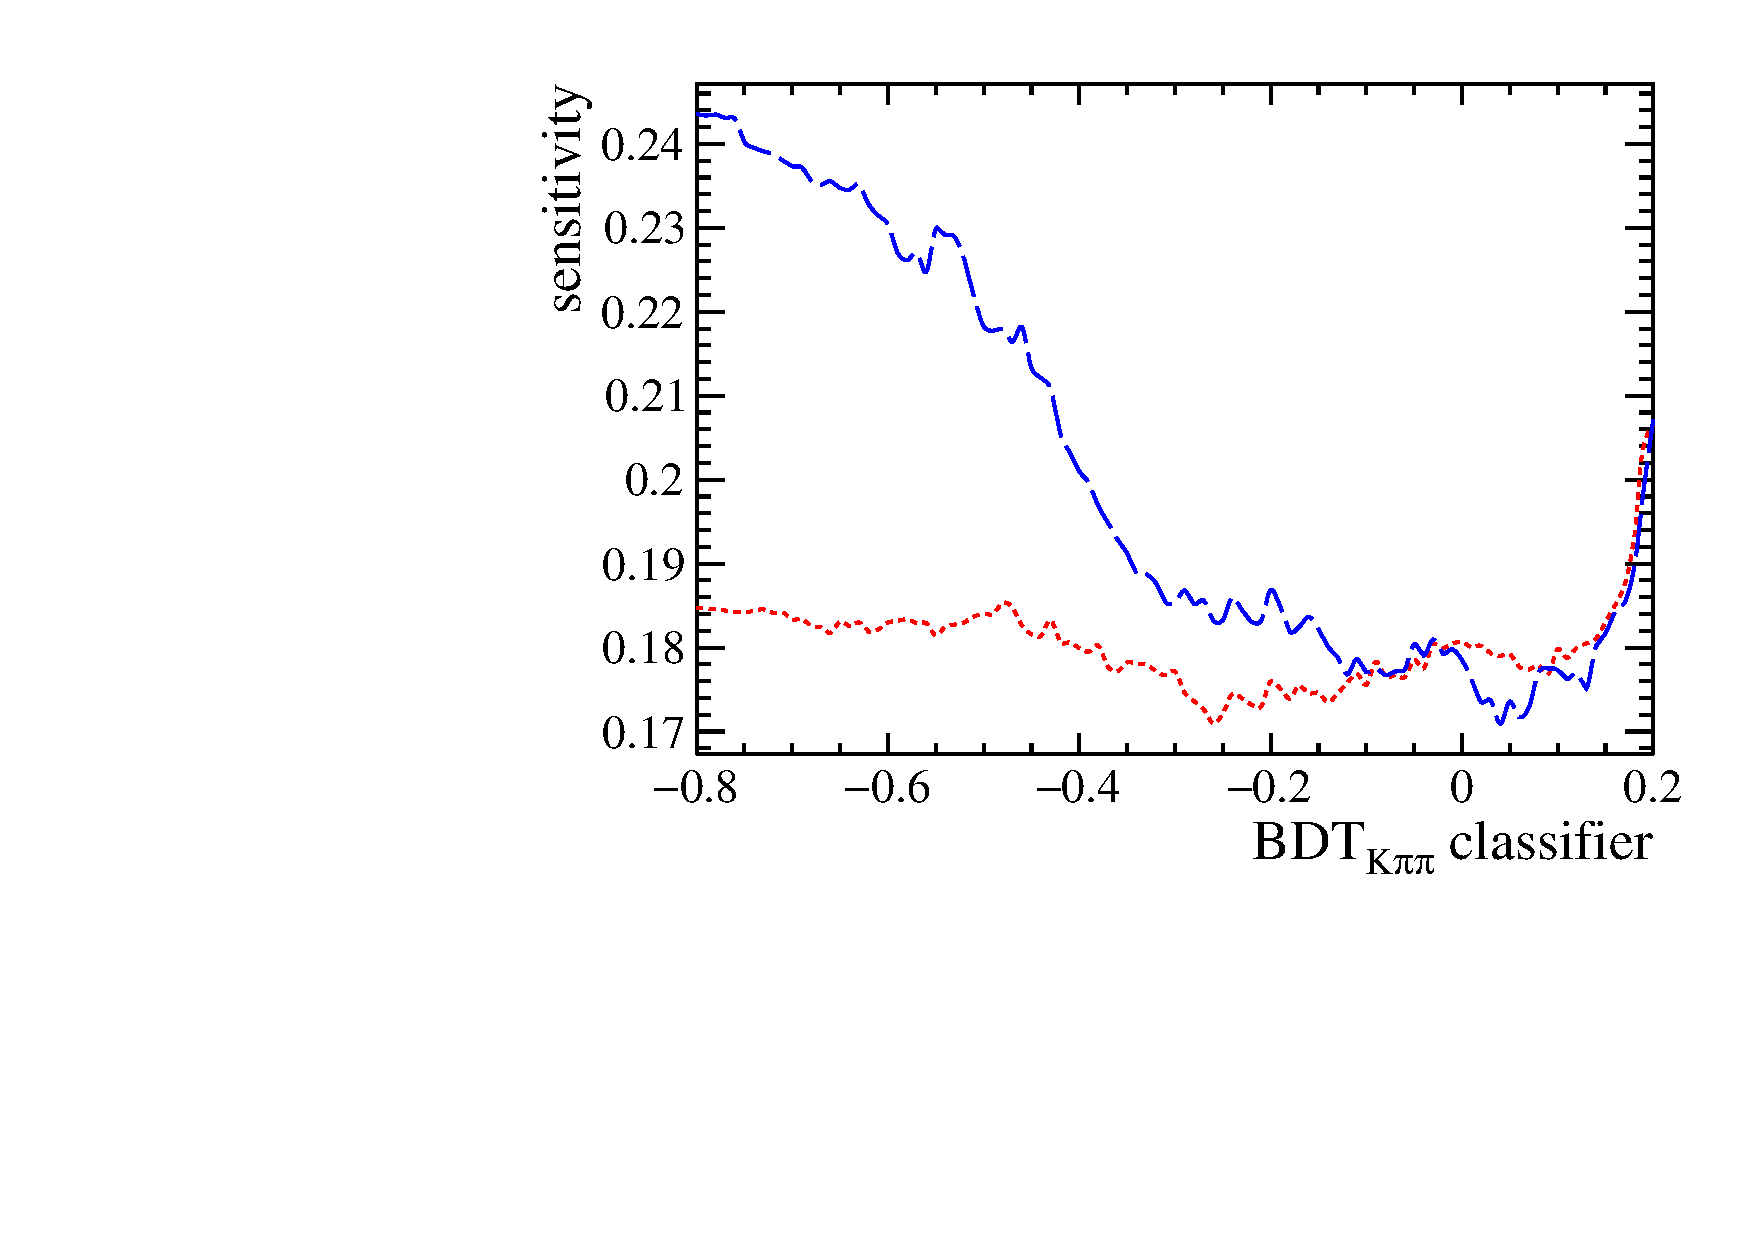
\includegraphics[width=0.48\textwidth]{07-B02DD/figs/Sensitivities_Kpipi.pdf}
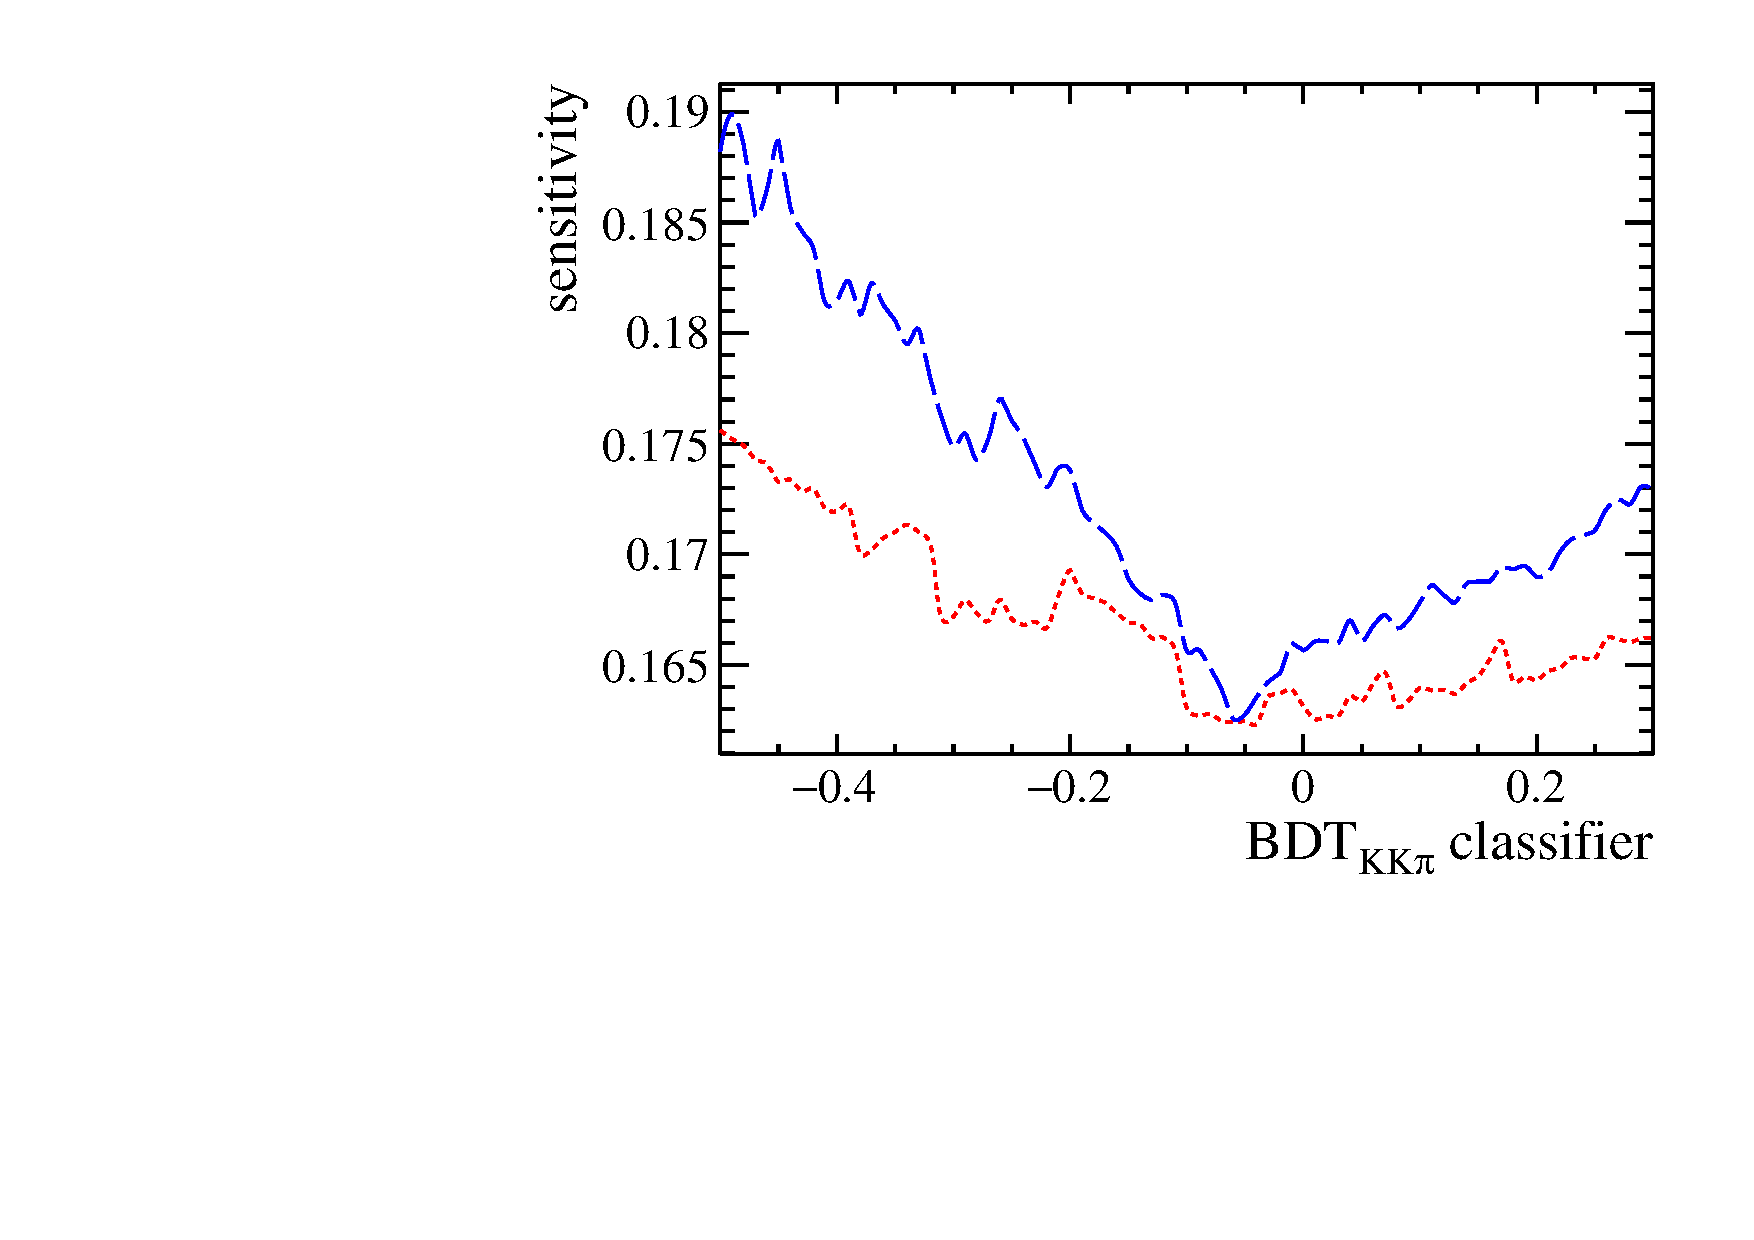
\includegraphics[width=0.48\textwidth]{07-B02DD/figs/Sensitivities_KKpi.pdf}
\caption{Sensitivity of \SDD (red short-dashed) and \CDD (blue long-dashed) as
a function of the BDT classifier output for the \KpipiKpipi final state (left)
and the \KKpiKpipi final state (right).}
\label{fig:b02dd:selection:mva:sensitivities}
\end{figure}
%
The uncertainty on \CDD improves with tighter requirements on the BDT
classifier until it reaches an optimum shortly after zero. This can be
explained with the fact that the sensitivity on \CDD mainly comes from
candidates at low decay times because the cosine function is maximal there.
The suppression of the rather short-lived combinatorial background compensates
the loss in signal efficiency for a quite long range. In contrast, the
uncertainty on \SDD is mainly driven by the amount of signal candidates. So it
is more or less flat for loose requirements on the BDT classifier where only
few signal candidates are lost and this is compensated by the higher purity
and reaches its optimum around \num{-0.25} before it starts to get worse. Now
that both observables are of interest and the optima are not at the same cut
value it is decided to require the BDT classifier to be greater than
\num{-0.10}. This is a good compromise between both observables as the
uncertainties of \SDD and \CDD are almost the same and close to their optima.
The requirement has a signal efficiency of \SI{96.5\pm0.5}{\percent} and
rejects \SI{84.18\pm0.34}{\percent} of the combinatorial background.

In a second step the requirement on the BDT classifier for the \KKpiKpipi
final state is optimised. The \KKpiKpipi subsample is quite small, which makes
individual fits on this subsample rather unstable. This can be solved by
performing a simultaneous fit to the whole dataset with the previously
determined BDT cut applied to the \KpipiKpipi subsample. Scanning the BDT
classifier output for the \KKpiKpipi final state results in the sensitivities
on \SDD and \CDD plotted in \cref{fig:b02dd:selection:mva:sensitivities}. Both
uncertainties show a minimum at around \num{-0.05}, which is chosen as cut
value. This cut removes \SI{90.75\pm0.33}{\percent} of the combinatorial
background at a signal efficiency of \SI{87.2\pm1.9}{\percent}.

\subsection{Final selection}
\label{sec:b02dd:selection:final_selection}

Finally, the fit range of the invariant $m_{\Dp\Dm}$ mass is reduced to
\SIrange{5150}{5500}{\MeVcc}, which eliminates some backgrounds, like
misreconstructed \mbox{\BdToDstD}, at low masses, prevents overtraining
effects on the high-mass sideband used in the training of the BDT, and leaves
enough candidates in the upper mass sideband to determine the shape of the
combinatorial background. Additionally, the decay time is restricted to be in
the range \SIrange{0.25}{10.25}{\ps} to avoid edge effects. In
\SI{0.8}{\percent} of the selected events more than one candidate remains,
which is very unlikely given the low branching branching fraction. So choosing
randomly only one of the multiple candidates is kept.


%!TEX root = ../main.tex

\subsection{Multivariate selection}
\label{sec:dataanalysis:selection:bdt}

More elaborate selection methods are based on machine learning algorithms,
which more and more enter the field of particle physics. These multivariate
techniques improve the possibility to separate signal from background
contributions as they make use of correlations between input variables.
Software packages, like TMVA~\cite{Hocker:2007ht} or
scikit-learn~\cite{scikit-learn}, provide implementations of these algorithms.

A simple multivariate classifier is a decision tree~\cite{Breiman}, which
splits the phase space according to repeated decisions on certain variables.
Starting from a root node the variable and cut value is determined, where the
best separation can be achieved according to a criterion like the Gini
index $p \cdot (1-p)$~\cite{giniindex}, with $p$ being the signal purity, \ie
the fraction of signal in the total data sample. At each following node the
cut value and even the variable used for the separation can be chosen
dependent on the previous decision. The depth of the tree, \ie the maximal
number of consecutive decisions, is tunable. When a stop criterion is matched,
\eg the ratio of candidates reaching a node falls below a predefined
threshold, no further decisions are applied. The tree is trained with a set of
labelled data. Each final leaf is classified as signal or background depending
on the class of the majority of training events ending in that leaf. Ideally,
the decision tree should learn, which sequence of criteria achieves the best
separation between signal and background. An improvement can be achieved by
combining several decision trees to a forest, in which the classification of
an event follows a majority vote of the individual trees, \eg in a Random
Forest~\cite{RandomForest}.

An alternative is to alter the impact of the training events in a decision
tree by applying weights. This procedure is called boosting and leads to
Boosted Decision Trees (BDT)~\cite{Roe}. One possibility how the
boosting can be realised is the AdaBoost method~\cite{AdaBoost}. Events that
are misidentified in the previous tree are weighted by
\begin{align}
	\alpha = \frac{1 - \eps}{\eps}\,,
\end{align}
with $\eps < \num{0.5}$ being the misclassification rate of the previous tree.
This criterion is fulfilled as long as the decision tree performs better than
a random choice. The learning rate can be further modified by using an
exponent $\beta$ for the weight, $\alpha \to \alpha^{\beta}$. To have the same
effective number of events as before, \ie the same sum of weights, the events
are renormalised before training the next tree. The BDT output classifier $y$
is given by the weighted mean of the tree's output $h$, which is \num{+1} for
signal and \num{-1} for background,
\begin{align}
	y = \frac{1}{N_{\textrm{trees}}} \sum_i^{N_{\textrm{trees}}} \ln(\alpha_i) h_i\,.
\end{align}
This means that an event is classified more signal-like the higher the BDT
output classifier. Another boosting algorithm is the GradientBoost
method~\cite{GradientBoost}. It is based on minimising a defined loss
function, which describes the deviation between the classification and the
truth, by calculating the gradient of the loss function.

The importance of a feature in a (boosted) decision tree can be determined by
counting how often it is used and by considering how important the cuts are in
terms of events reaching the corresponding node and in terms of the separation
power between signal and background candidates.

Another multivariate method is the Artificial Neural Network
(ANN)~\cite{Denby:1987rk}. It consists of several neurons, divided into input
units, hidden units and output units. The way how these units are connected,
the corresponding strength and the effect, either excitatory or inhibitory,
defines the neural network.

Multivariate selection methods have the disadvantage that their success has to
be limited or in other words that it is not necessarily ideal if a perfect
separation is achieved. The problem is that the training data are only proxies
for the real data and that the multivariate method eventually learns to
distinguish the different categories based on unphysical properties that do
not inhere in real data. These could for example be statistical fluctuations
or differences between simulated and real data. This so called overtraining
leads to an overestimation of the performance of the selection. Overtraining
can be avoided if the training data samples are large and as close as possible
to the real data, on which the selection should be applied in the end.
However, this does not mean that the same data should be used for the training
and for the analysis. In the selection of \BdToDD decays the high mass
sideband is taken as proxy for the combinatorial background and excluded from
the subsequent analysis. A typical check for overtraining is performed by
comparing the output classifier distributions of the training data and of a
test sample, which has been removed randomly from a common data set.

%!TEX root = ../main.tex

\subsection{Unfolding data distributions using \texorpdfstring{$\sWeights$}{sWeights} (1 page)}
\label{sec:dataanalysis:selection:splot}

%!TEX root = ../main.tex

\subsection{Figures of merit}
\label{sec:dataanalysis:selection:fom}

One of the main questions when performing a selection is, how the
requirements, be it a sequence of cuts or the classifier of a multivariate
method, should be optimized. In an ideal world, one would find a selection
that keeps all signal candidates and removes all background contributions. But
this is unrealistic. Instead, suitable figures of merit have to be defined,
whose optimum should correspond with the ideal selection.  In a measurement of
\CP violation the goal is to obtain the optimal precision. Therefore, the
sensitivity on the \CP observables itself seems to be the best figure of
merit. However, there are some caveats. On the one hand there is usually more
than one observable describing the \CP violation and a strategy needs to be
found how the sensitivities of the different \CP observables can be combined
into a single figure of merit. On the other hand the absolute uncertainty
might depend on the central value and thus small values for the \CP
observables could be preferred. Finally, the full time-dependent fit has to be
performed, which is often very complex and takes a long time until it
converges. For all these reasons, alternative figure of merits are developed.
A very simple one is the pure signal efficiency $\epsilon_S$. Under the
assumptions that a high signal yield is more important than a low background
contamination and that the selection requirements are effectively suppressing
background contributions, a possible selection strategy is to judge
requirements only by their signal efficiency. In the \BdToJPsiKS analysis this
approach is chosen using the requirement that the individual cuts have to be
at least \SI{99}{\percent} signal efficient. Including the background yield to
the definition of the figure of merit should make it easier to find the
optimal cut point, as the background contamination partly influences the
achievable sensitivity. There are several possibilities how the signal yield
$S$ and the background yield $B$ can be combined: The figure of merit
\begin{align}
	Q_1 = \frac{S}{S + B}\,,
\end{align}
called purity, describes the fraction of signal candidates. It is limited to
unity, which is reached when no background candidates are left over. Using
merely the purity does not necessarily lead to an optimal selection, \eg when
lots of signal candidates would be thrown away in order to remove one last
remaining background candidate. Instead, the signal significance
\begin{align}
	Q_2 = \frac{S}{\sqrt{S + B}}\,,
\end{align}
which states by how many standard deviations the signal yield exceeds zero, is
widely used. To enhance the impact of a high signal yield, the signal
significance can be multiplied with the purity:
\begin{align}
	Q_3 = \frac{S^2}{\sqrt{(S + B)^3}}\,.
\end{align}
For decay-time-independent studies, like determinations of branching ratios,
the figure of merit $Q_3$ is appropriate. In searches for very rare decay
modes, where a certain significance expressed in number of standard deviations
$a$ is desired, Punzi's figure of merit~\cite{Punzi:2003bu}
\begin{align}
	Q_4 = \frac{\epsilon_S}{a/2 + \sqrt{B}}\,,
\end{align}
is often used.

However, for decay-time-dependent studies the figure of merit can be improved
through an extension that takes into account that the contribution of a signal
candidate to the sensitivity on \CP observables depends on its decay time. For
instance, the sine term in the decay-time-dependent asymmetry (see
\cref{eq:cpviolation:simpleasymmetry} has its maximum at $t =
\frac{\pi}{2\,\dmd} \approx \SI{3}{\ps}$. Thus, signal candidates with such
decay times have a higher impact. This can be expressed by adding up the
square of the differentiation of the log-likelihood with respect to the
parameter of interest, here $\Sf$, of all $N_S$ signal candidates:
\begin{align}
	Q_5 = \sum_{i=1}^{N_S} \left[\frac{\sin(\dmd\,t_i)}{1 + d_i\,S_f\,\sin(\dmd\,t_i)}\right]^2\,,
\end{align}
with $d_i = \num{+1}$ for \Bd and $d_i = \num{-1}$ for \Bdb. Additionally, it
has to be considered that the decay time distribution of background candidates
usually follows an exponential function with an effective lifetime that is
significantly smaller than the \Bd signal lifetime. This can be incorporated
by using a decay-time-dependent purity $f_i(t)$:
\begin{align}
	Q_6 = \sum_{i=1}^{N} f_i^2 \cdot \left[\frac{\sin(\dmd\,t_i)}{1 + d_i\,S_f\,\sin(\dmd\,t_i)}\right]^2\,.
\end{align}
Here, the sum is built over all $N$ candidates, signal and background. The
purity can be determined via a fit to the invariant mass distribution or more
specifically via sWeights (see \cref{sec:dataanalysis:selection:splot}).
Moreover, the influence of further experimentally induced dilutions can be
added, \eg from the flavour tagging (see \cref{sec:detector:tagging})
or the decay time resolution (see \cref{sec:dataanalysis:resolution}). Such a
generalized figure of merit for decay-time-dependent measurements of
\CP violation is derived in Ref.~\cite{FOM}.

%!TEX root = ../main.tex

\section{Spline interpolation (0.5 pages)}
\label{sec:dataanalysis:splines}

In many cases phenomenological models are an efficient way of describing
shapes, \eg when parametrising acceptances, which are typically influenced by
more effects than could realistically be analysed separately. Interpolating
cubic splines, which are piecewise defined polynomials of degree three, are an
useful implementation~\cite{Splines}. They are parametrised by a set of knots
and coefficients at these positions and can be written as the sum over base
splines. The first and second derivatives are continuous throughout the
domain. The choice of the number and positions of the knots determines how
accurate the given shape can be described.

In this thesis cubic splines are used to parametrise the shape of mistag
distributions and to transfer a histogram of the decay-time-dependent
efficiency into an unbinned, analytically integrable representation in the
\BdToJPsiKS analysis, and to model the deviation of the decay time
distribution from a pure exponential distribution in the \BdToDD analysis.

%!TEX root = ../main.tex

\section{Bootstrapping method (0.5 pages)}
\label{sec:dataanalysis:bootstrapping}

The bootstrapping method (see \eg \cite{Behnke:2013pga}) is a frequentist
model-independent approach to estimate confidence level intervals. Toy data
samples are produced by drawing events from the nominal data sample, with
replacement, until the statistics matches the number of candidates of the
nominal data sample. This means that the same event can be drawn multiple
times. The toy data samples serve as test samples on which all calculations or
fits that are done on the nominal data sample can be repeated several times.
\todo{extend bootstrapping, advantages, ...}

%!TEX root = ../main.tex

\section{Blinding}
\label{sec:dataanalysis:blinding}

To eliminate the experimenter's bias, a blinding transformation is applied on
the fitted \CP parameters \SDD and \CDD with the
\verb|RooUnblindUniform| method of \roofit's \verb|RooBlindTools|~\cite{roofit}.
The transformation implemented in the \verb|RooUnblindUniform| method adds a
hidden offset to the fit parameter. Doing so, the uncertainty on the extracted
parameter does not change and can still be used for understanding the outcome of
the fit. The hidden offset is drawn from a uniform distribution with a range
$\pm s$, using a random number generator with known seed. The seed is generated
from a so-called \emph{blinding string}. If two different analyses of the same
physics parameter agree on a common scale and blinding string, then the results
of those analyses can be compared without unblinding. We choose the range of the
uniform distribution to be $[-2,2]$. Given the physical range of \sintwobeta is
$[-1,1]$, this ensures a good opacity.
\todo{rewrite blinding}

%!TEX root = ../main.tex
\section{Decay time resolution}
\label{sec:dataanalysis::resolution}

Uncertainties in the determination of the position of vertices and in the
measurement of momenta (although thanks to the VELO (see
\cref{sec:detector:lhcb}) pretty accurate  at $\lhcb$) lead to a finite decay
time resolution $\sigma$, which dilutes the observed $\CP$ asymmetry by a
factor
\begin{align}
  \mathcal{D} = e^{\frac{-\dmd^2\,\sigma^2}{2}} \, .
\end{align}
This formula is the special case for a Gaussian resolution model with width
$\sigma$. The general formula is derived in
Ref.~\cite{ResolutionDilutionFactor}. For $\Bd$ mesons the dilution induced by
the decay time resolution has only minor influence on the measurement of $\CP$
observables because the oscillation frequency of $\Bd$ mesons $\dmd =
\SI{0.5064\pm0.0019}{\hbar\invps}$~\cite{HFAG} is quite low. Even for a decay time
resolution of \SI{100}{\fs}, which would be almost two times larger than what
is usually found in analyses performed by \lhcb, the dilution factor is
greater than \SI{99}{\percent}.

%!TEX root = ../main.tex

\section{Flavour tagging calibration (1 page)}
\label{sec:dataanalysis:taggingcalibration}

%!TEX root = ../main.tex

\subsection[Calibration using \texorpdfstring{$\BdToDsD$}{Bd2DsD} (2 pages)]{Calibration using \texorpdfstring{$\BdToDsD$}{Bd2DsD}}
\label{sec:dataanalysis:taggingcalibration:dsdcalibration}

\begin{table}[!htb]
\caption{Flavour tagging calibration parameters from \BdToDsD. The first
uncertainty is statistical and the second accounts for systematic
uncertainties.}
\label{tab:dataanalysis:taggingcalibration:dsdcalibration}
\centering
\begin{tabular}{lr@{$\,\pm\,$}l@{$\,\pm\,$}lr@{$\,\pm\,$}l@{$\,\pm\,$}l}
  \toprule
  Parameter           & \multicolumn{3}{c}{OS}   & \multicolumn{3}{c}{SS} \\
  \midrule
  $p_{1}$               & 1.069   & 0.072  & 0.01  & 0.842   & 0.090  & 0.01  \\
  $p_{0}$               & 0.3691  & 0.0080 & 0.01  & 0.4296  & 0.0060 & 0.009 \\
  $\langle \eta\rangle$ & \multicolumn{3}{c}{0.3627} & \multicolumn{3}{c}{0.4282} \\
  $\Delta p_{1}$        & 0.03    & 0.11   & 0.03  & 0.07    & 0.13   & 0.05  \\
  $\Delta p_{0}$        & 0.009   & 0.012  & 0.001 & -0.0065 & 0.0087 & 0.001 \\
  \bottomrule
\end{tabular}
\end{table}

%!TEX root = ../main.tex

\subsection{Calibration using \texorpdfstring{$\JPsiX$}{JpsiX} channels}
\label{sec:dataanalysis:taggingcalibration:jpsixcalibration}

For the charged $\BuToJPsiK$ decay, which is used to determine the calibration
of the OS tagging combination for the analysis of \BdToJPsiKS decays, a
comparison of the charge of the kaon with the tag decision directly tells if
the tag decision is correct or not. Binning the sample in terms of the mistag
estimate a \chisq fit using
\cref{eq:dataanalysis:taggingcalibration:generalfunction} is performed to the
($\eta$, $\omega)$ pairs and reveals the following results for the calibration
parameters:
\begin{equation}
\begin{aligned}
  p_0^{\text{OS}} &= 0.3815 \pm 0.0011 \text{\,(stat.)}
                            \pm 0.0016 \text{\,(syst.)} \, ,\\
  p_1^{\text{OS}} &= 0.978\phantom{0} \pm 0.012\phantom{0} \text{\,(stat.)}
                                      \pm 0.009\phantom{0} \text{\,(syst.)} \, ,\\
  \langle\eta^{\text{OS}}\rangle &= 0.3786 \, .
\end{aligned}
\label{eq:dataanalysis:taggingcalibration:jpsixcalibration:os_calibration_pars}
\end{equation}
Repeating the same fit with a split of the sample into the initial flavours
gives access to the asymmetry parameters $\Delta p_0$ and $\Delta p_1$, which
are determined to be
\begin{equation}
\begin{split}
  \Delta p_0^{\text{OS}} &= 0.0148 \pm 0.0016 \text{\,(stat.)} \pm  0.0008 \text{\,(syst.)} \, , \\
  \Delta p_1^{\text{OS}} &= 0.070\phantom{0} \pm 0.018\phantom{0} \text{\,(stat.)} \pm 0.004\phantom{0} \text{\,(syst.)} \,.
\end{split}
\label{eq:dataanalysis:taggingcalibration:jpsixcalibration:os_calibration_asymmetries}
\end{equation}
A cross-check of the calibration in a control sample of $\BdToJPsiKstar$
decays confirms the validity of transferring the calibration from $\Bu$ to
$\Bd$ decays.

Despite the advantages of $\BuToJPsiK$ as control channel (charged decay mode,
very high statistics), for the calibration of the cut-based SS\pion tagging
algorithm \mbox{$\BdToJPsiKstar$} decays are used because differences in the
composition of the fragmentation products in the $\Bp$ and $\Bz$ hadronisation
are expected. Like for \BdToDsD a time-dependent mixing analysis is needed.
Here, a two dimensional fit to both the reconstructed decay time and mass
distributions is performed. From a simultaneous fit in five evenly filled bins
of the mistag estimate $\eta$ the calibration parameters for the SS\pion
tagging algorithm are determined to be
\begin{equation}
\begin{aligned}
  p_0^{\text{SS\pion}}        &=& \phantom{+}0.4232  &\pm\, 0.0029 \text{\,(stat.)} &\pm\, 0.0028 \text{\,(syst.)} \, ,\\
  p_1^{\text{SS\pion}}        &=& \phantom{+}1.011\phantom{0}   &\pm\, 0.064\phantom{0} \text{\,(stat.)} &\pm\, 0.031\phantom{0} \text{\,(syst.)} \, ,\\
  \Delta p_0^{\text{SS\pion}} &=& -0.0026 &\pm\, 0.0043 \text{\,(stat.)} &\pm\, 0.0027 \text{\,(syst.)} \, , \\
  \Delta p_1^{\text{SS\pion}} &=& -0.171\phantom{0}   &\pm\, 0.096\phantom{0} \text{\,(stat.)} &\pm\, 0.04\phantom{00} \text{\,(syst.)} \, , \\
  \langle\eta^{\text{SS\pion}}\rangle        &=& \phantom{+}0.425\phantom{0} & .
\end{aligned}
\label{eq:dataanalysis:taggingcalibration:jpsixcalibration:ss_calibration_pars}
\end{equation}

The systematic uncertainties for both calibrations cover two different types,
one for intrinsic uncertainties and one for the kinematic differences between
the control mode and the signal decay \BdToJPsiKS. The effect of these two
sources is of the same order.

The combined effective tagging efficiency is \SI{3.02\pm0.05}{\percent}, which
is composed of a tagging efficiency of \etag = \SI{36.54\pm0.14}{\percent} and
an effective mistag probability of $\mistag_{\textrm{eff}} =
\SI{35.62\pm0.12}{\percent}$. The major contribution comes from the OS tagging
combination, which has an inclusive tagging power of
\SI{2.63\pm0.04}{\percent}. The cut-based SS\pion tagging algorithm adds
\SI{0.376\pm0.024}{\percent}.

%!TEX root = ../main.tex

\chapter[Measurement of \texorpdfstring{$\CP$}{CP} Violation in \texorpdfstring{$\BdToJPsiKS$}{Bd2JPsiKS} Decays (10 pages)]{Measurement of \texorpdfstring{$\CP$}{CP} Violation in \texorpdfstring{$\BdToJPsiKS$}{Bd2JPsiKS} Decays}
\label{sec:bd2jpsiks}

%!TEX root = ../main.tex

\section{Data Preparation (1 page)}
\label{sec:bd2jpsiks:datapreparation}

%!TEX root = ../main.tex
\section{Decay time resolution}
\label{sec:bd2jpsiks:decaytime:resolution}

The most obvious effect of the decay time resolution are candidates that are
reconstructed with negative decay times. However, these are ideal candidates
to determine the decay time resolution. An unbinned likelihood fit to the
decay time distribution of an unbiased \BdToJPsiKS sample with true \jpsi
candidates (selected by a fit of the invariant $m_{\mumu}$ mass distribution)
is performed. The fit model consists of a component for the prompt peak around
\SI{0}{\ps}, \ie the decay time resolution model, a component to describe
events where the wrong PV has been associated and therefore a large difference
between true and reconstructed decay time occurs, and long lived components,
which are parametrised with two exponentials with different pseudo lifetimes,
and which are themselves convolved with the decay time resolution model. The
decay time resolution depends on characteristics of the event. The DTF
provides predictions for the per-event decay time resolution $\sigma_t$, which
in principle could be used as width of a Gaussian resolution model.
Unfortunately, these predictions are not perfect and a certain calibration
needs to be applied. Additionally, to account for different sources causing
the decay time resolution an effective model with two Gaussian functions, which
share a common mean but have different calibrations, is used.

The first step is to find a reasonable calibration model. A linear ($f_1$) and
a quadratic ($f_2$) calibration model are tested:
\begin{equation}
\begin{aligned}
f_1:&\quad \sigma_{\text{true}}(\sigma_t) &=&  &b_i\,\sigma_t &+ c_i \ , \\
f_2:&\quad \sigma_{\text{true}}(\sigma_t) &=&\, \alpha_i\,\sigma_t^2 + &\beta_i\,\sigma_t &+ \gamma_i \ .
\end{aligned}
\label{eq:resolutioncalibfunctions}
\end{equation}
%
The data sample is divided into \num{20} equally filled bins of the decay time
resolution predictions $\sigma_t$. This is done separately for the downstream
and the long track sample as the decay time resolution of long track
candidates is expected to be significantly better. Under the assumption that
$\sigma_t$ is constant inside the bins average widths can be set for the two
Gaussian functions. An unbinned likelihood fit to the decay time distribution,
simultaneous to all bins, sharing all fit parameters except the widths of the
Gaussian resolution functions is performed. The widths are plotted in the
corresponding bins and a \chisq-fit with the two calibration functions is
executed. For the downstream sample the results are depicted in
\cref{fig:CalibrationOffsetResolution_DD}. \todo{replace plots with different line styles}
%
\begin{figure}[!htb]
\centering
  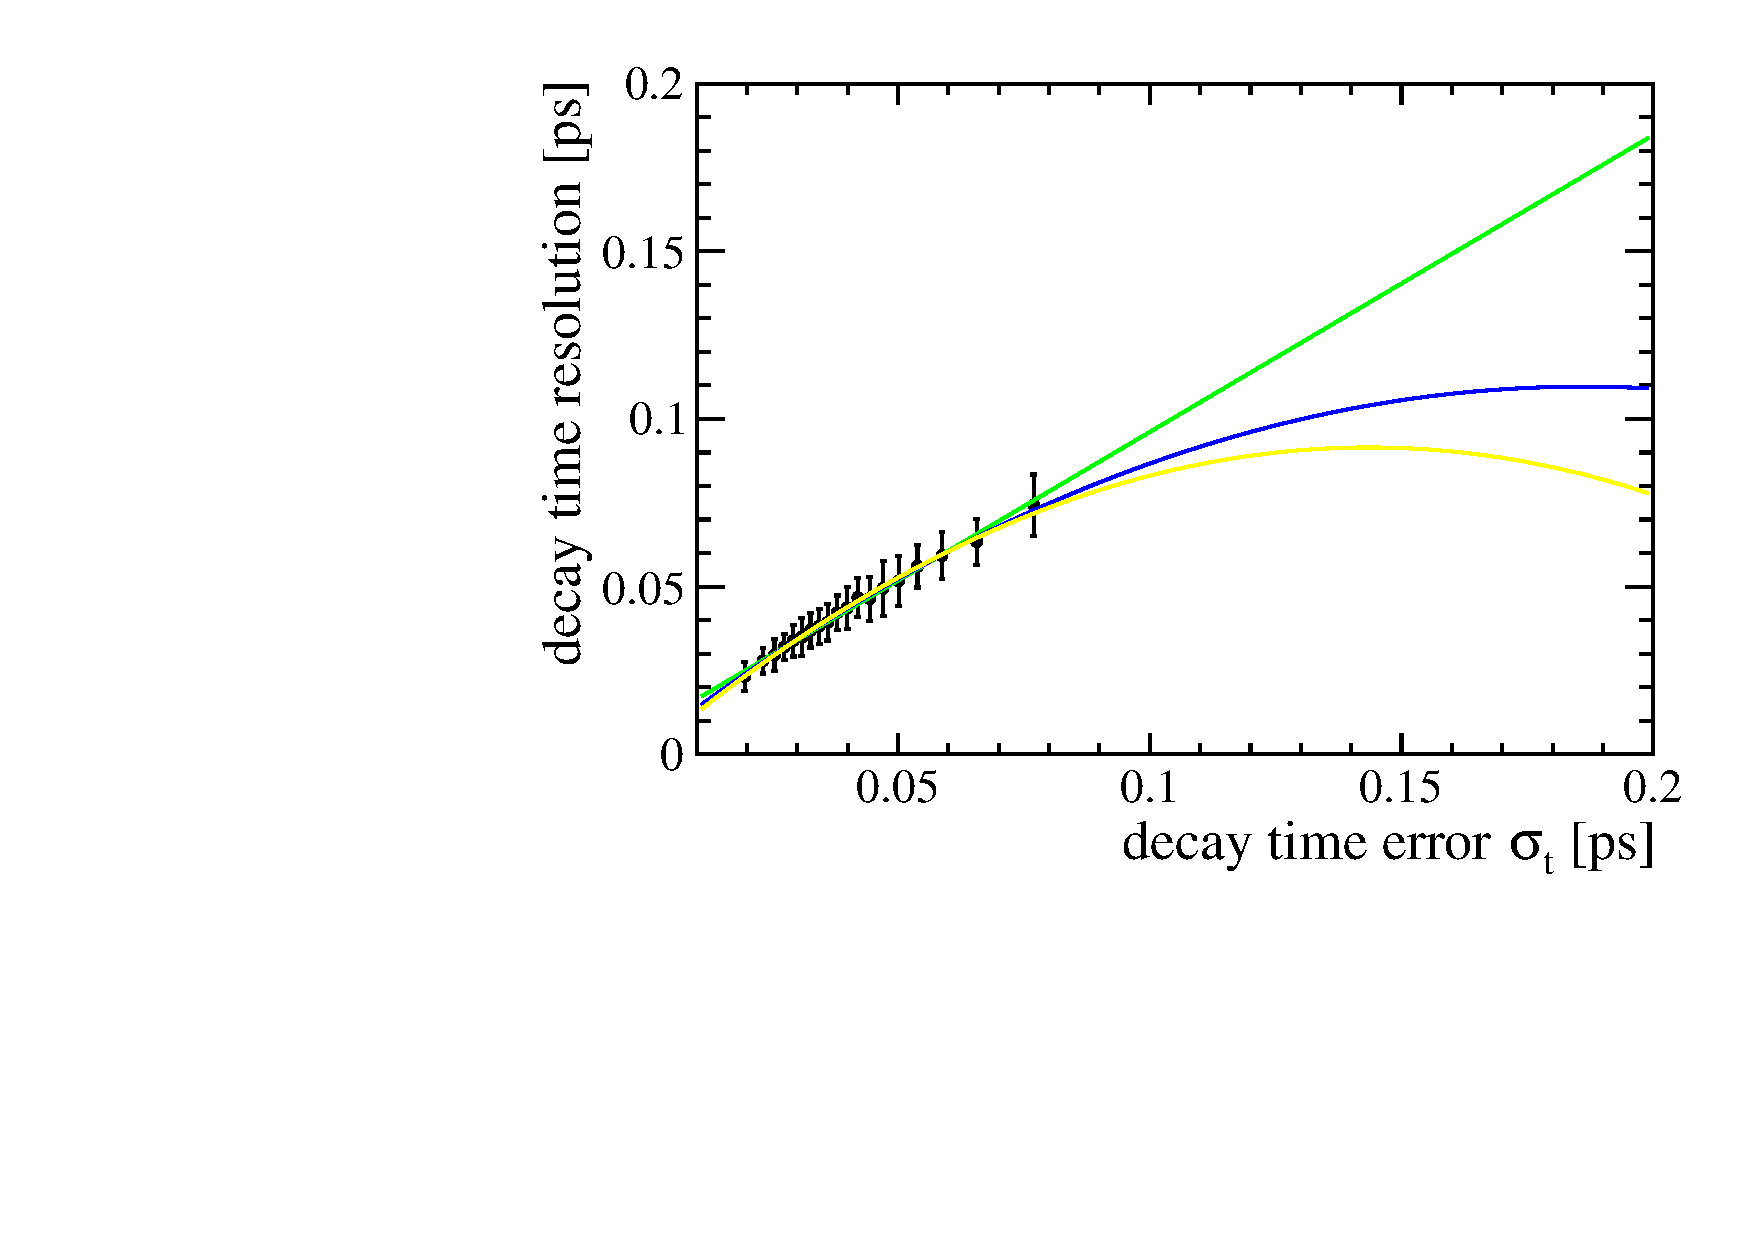
\includegraphics[width=0.45\textwidth]{06-Bd2JpsiKS/figs/ResolutionCalibration_1_DD.pdf}
  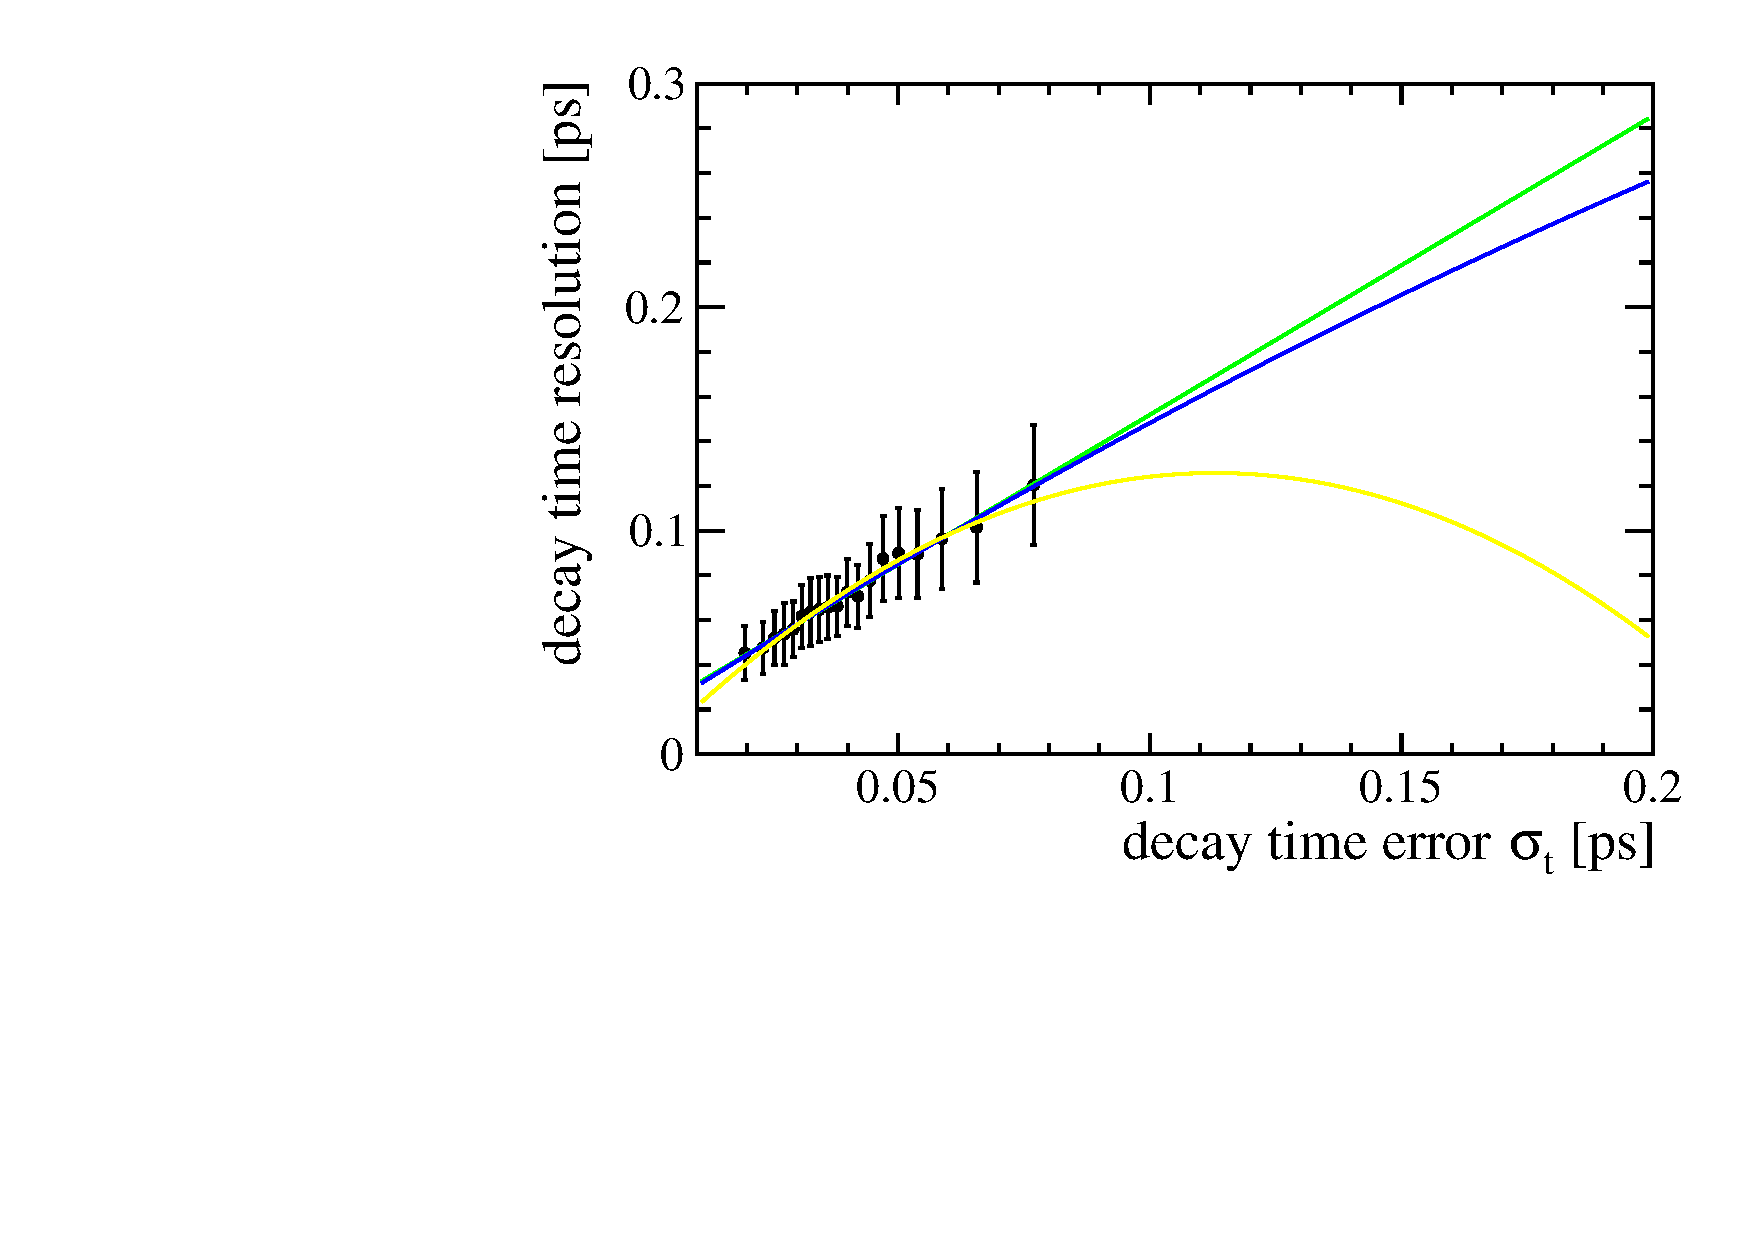
\includegraphics[width=0.45\textwidth]{06-Bd2JpsiKS/figs/ResolutionCalibration_2_DD.pdf}
\caption{Fit of a linear (green) and a quadratic calibration function (blue)
to the narrower (left) and to the wider width (right) of the downstream
sample. Fixing the offset of the quadratic function to zero (yellow) results
in an unphysical shape.}
\label{fig:CalibrationOffsetResolution_DD}
\end{figure}
%
Both functions fit equally well so the simpler linear model with less degrees
of freedom is preferred. The liner model is also chosen for the long track
sample.

With the calibration functions at hand a likelihood fit unbinned in decay
times and decay time resolution predictions is performed and the nominal
values of the calibration parameters are determined. The dilution factor
induced by the decay time resolution is calculated to be \num{0.986} for
downstream and \num{0.989} for long track candidates.

\section{Decay time acceptance}
\label{sec:bd2jpsiks:decaytime:acceptance}

The trigger line requirements applied in the selection of the \BdToJPsiKS
candidates partially bias the decay time distribution. The sample is divided
into an \emph{almost unbiased} subset and an \emph{exclusively biased} subset.

%!TEX root = ../main.tex

\section{Backgrounds (2 pages)}
\label{sec:bd2jpsiks:backgrounds}

Although \BdToJPsiKS is an experimentally very clean decay channel care has to
be taken to properly identify, suppress or even reject backgrounds. While the
two muons can be identified quite effectively the pions of the \KS decay might
actually be kaons or protons which have been mis-identified. This would lead
to background contributions from \BdToJPsiKst and \LbToJPsiL. To analyse the
$\proton \to \pion$ mis-ID the proton mass hypothesis is assigned to one of
the pions and the invariant mass of the proton-pion pair $m_{\proton\pion}$ is
recalculated. An excess of candidates at the \Lz mass $M_{\Lz} =
\SI{1115.683}{\MeVcc}$~\cite{PDG2014} can be seen which is reduced by applying
a tighter requirement on the difference of the proton-pion log-likelihood for
candidates close to $M_{\Lz}$. With \LbToJPsiL signal MC it is checked that
after reconstruction, stripping and all offline selection requirements,
including the veto described above, the expected yield is a sub-percent
effect. For $\kaon \to \pion$ mis-ID the broad width of the \Kstarz does not
allow an analogous approach. But studies on \BdToJPsiKst MC show that the
expected contribution is even lower than for \LbToJPsiL. The main reason is
the short lifetime of the \Kstarz which is exploited by the lifetime
significance cut on the \KS. So, it can basically be assumed that besides the
signal candidates almost only combinatorial background is present in the data
sample. Nevertheless, it has to be studied whether the background shows any
tagging-dependent asymmetry which would dilute the measured \CP asymmetry.

By performing a fit to the invariant mass distribution the \sPlot technique
provides a possibility to study the tagging-dependent distributions of the
combinatorial background. First of all, the time-integrated asymmetry
\begin{align}
  \mathcal{A}_\text{bkg}^{\text{int}} = \frac{\param{N}{\Bzb}{bkg} - \param{N}{\Bz}{bkg}}{\param{N}{\Bzb}{bkg} + \param{N}{\Bz}{bkg}}
\end{align}
is calculated for both track type categories and separately for the OS
combination and the SS\pion tagger. Out of the four values listed in
\cref{tab:bkgtimeintegratedasymm} only the one for the downstream OS tagged
sample which has the highest statistics stands out as it disfavours \CP
symmetry at more than \num{3} standard deviations.
%
\begin{table}[!htb]
\centering
\caption{Time-integrated asymmetry of sweighted background distributions for
downstream and long track OS and SS\pion tagged events.}
\label{tab:bkgtimeintegratedasymm}
\begin{tabular}{lr@{$\,\pm\,$}l}
	\toprule
category    & \multicolumn{2}{c}{$\mathcal{A}_\text{bkg}^{\text{int}}$}\\
\midrule
DD OS       & $0.017$     & $0.005$ \\
DD SS\pion  & $-0.016$    & $0.011$ \\
LL OS       & $-0.005$    & $0.012$ \\
LL SS\pion  & $0.044$     & $0.034$ \\
\bottomrule
\end{tabular}
\end{table}
%
But even time-integrated asymmetries compatible with zero do not exclude
time-dependent asymmetries. The latter are investigated by dividing the data
sample in ten bins of the decay time. The bin size is chosen to increase
exponentially. In \cref{fig:background_asymmetry_sweighted} again the four
categories of before are plotted.
%
\begin{figure}[!htb]
\centering
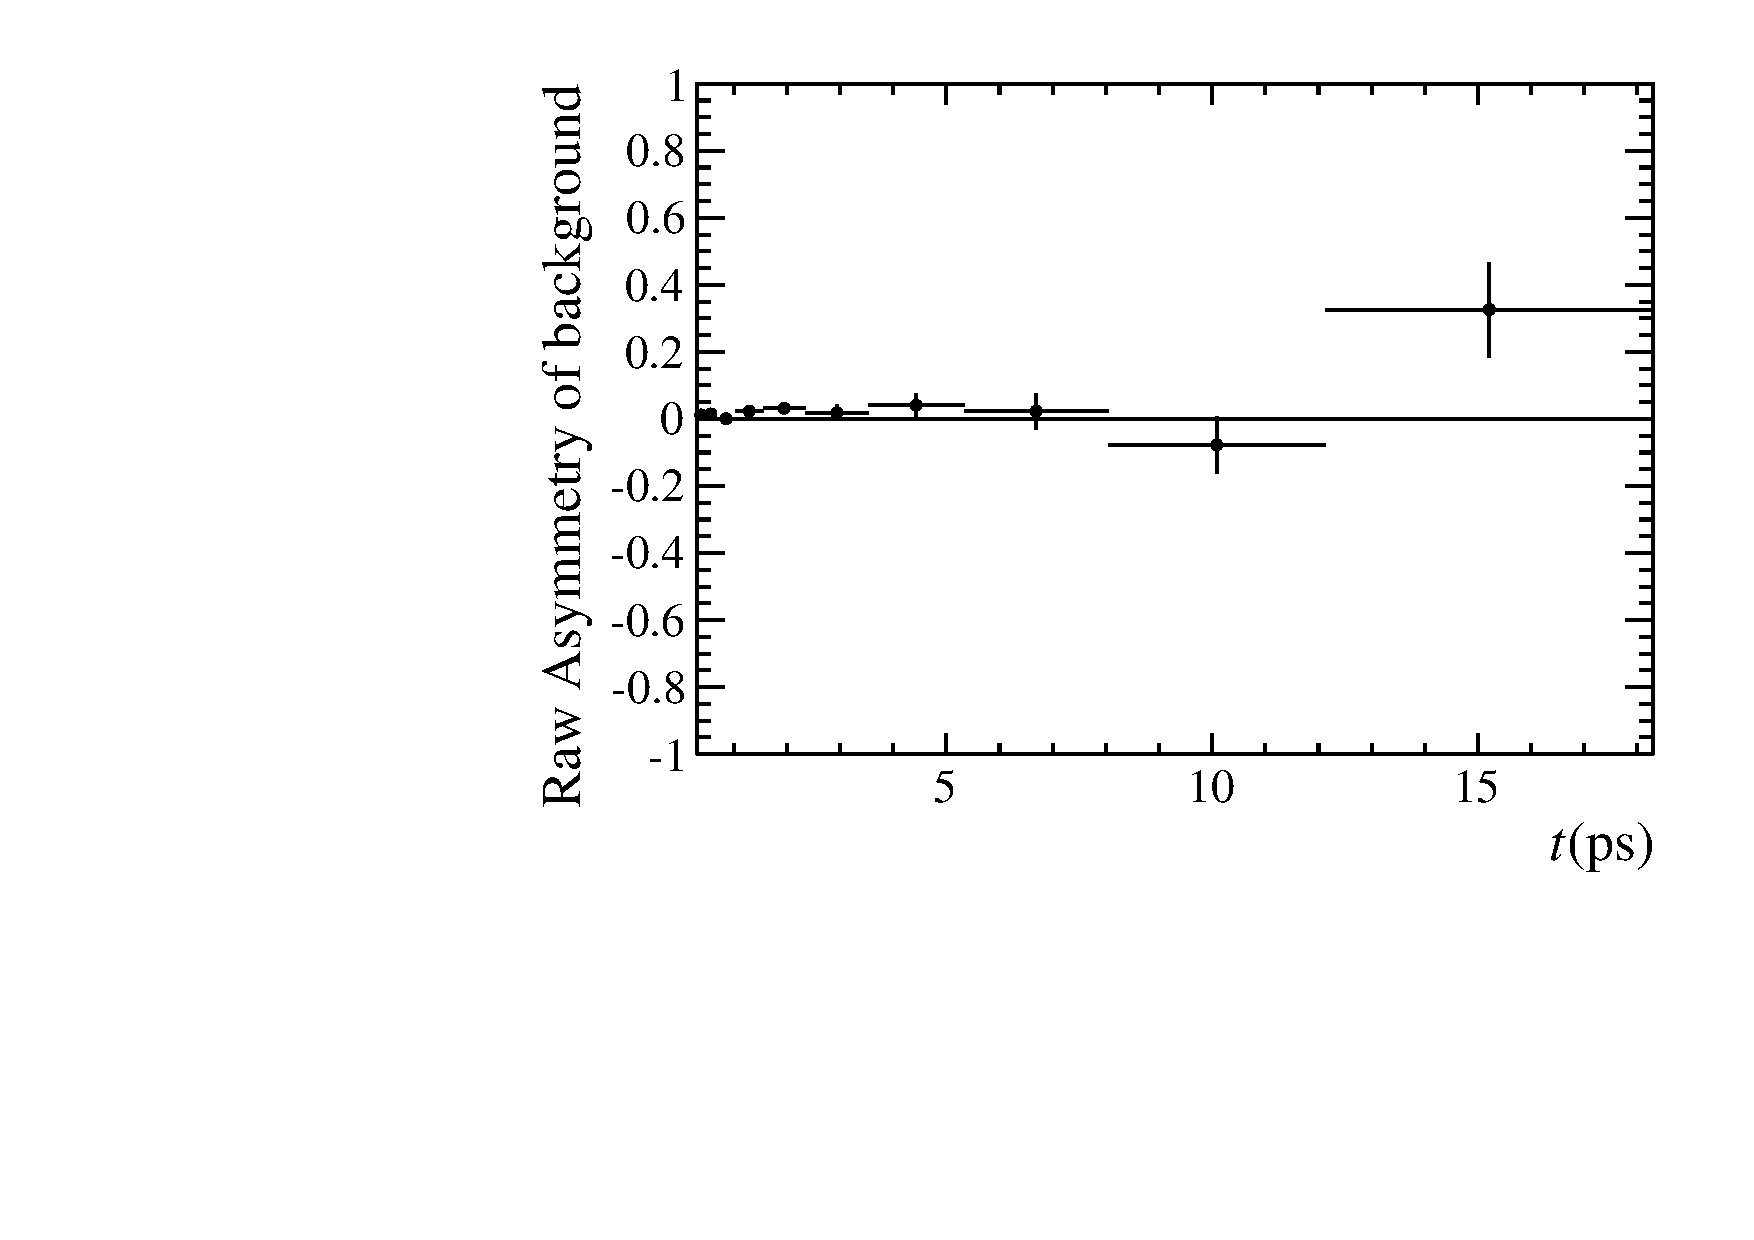
\includegraphics[width=0.49\textwidth]{06-Bd2JpsiKS/figs/BackgroundAsymmetryByHand_DD_OS_data.pdf}
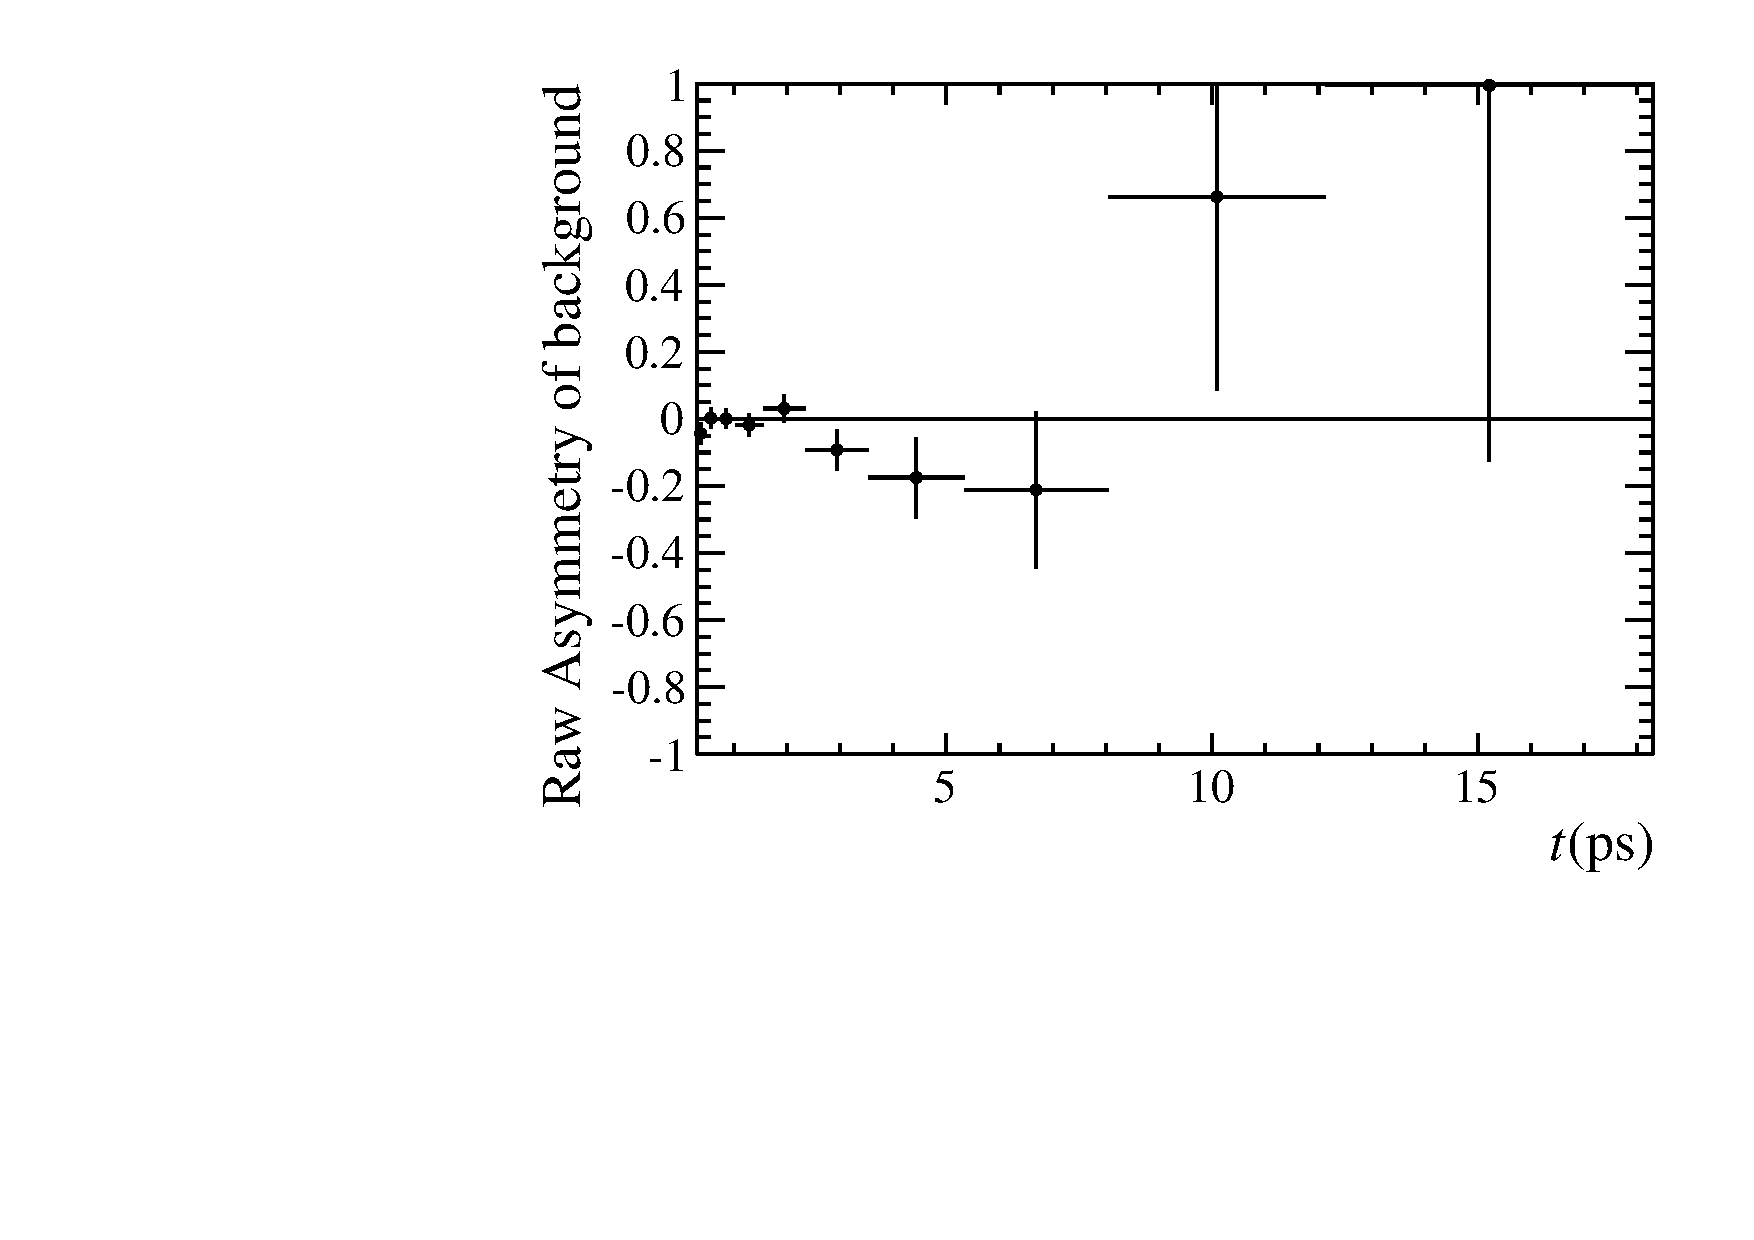
\includegraphics[width=0.49\textwidth]{06-Bd2JpsiKS/figs/BackgroundAsymmetryByHand_DD_SSPion_data.pdf}\\
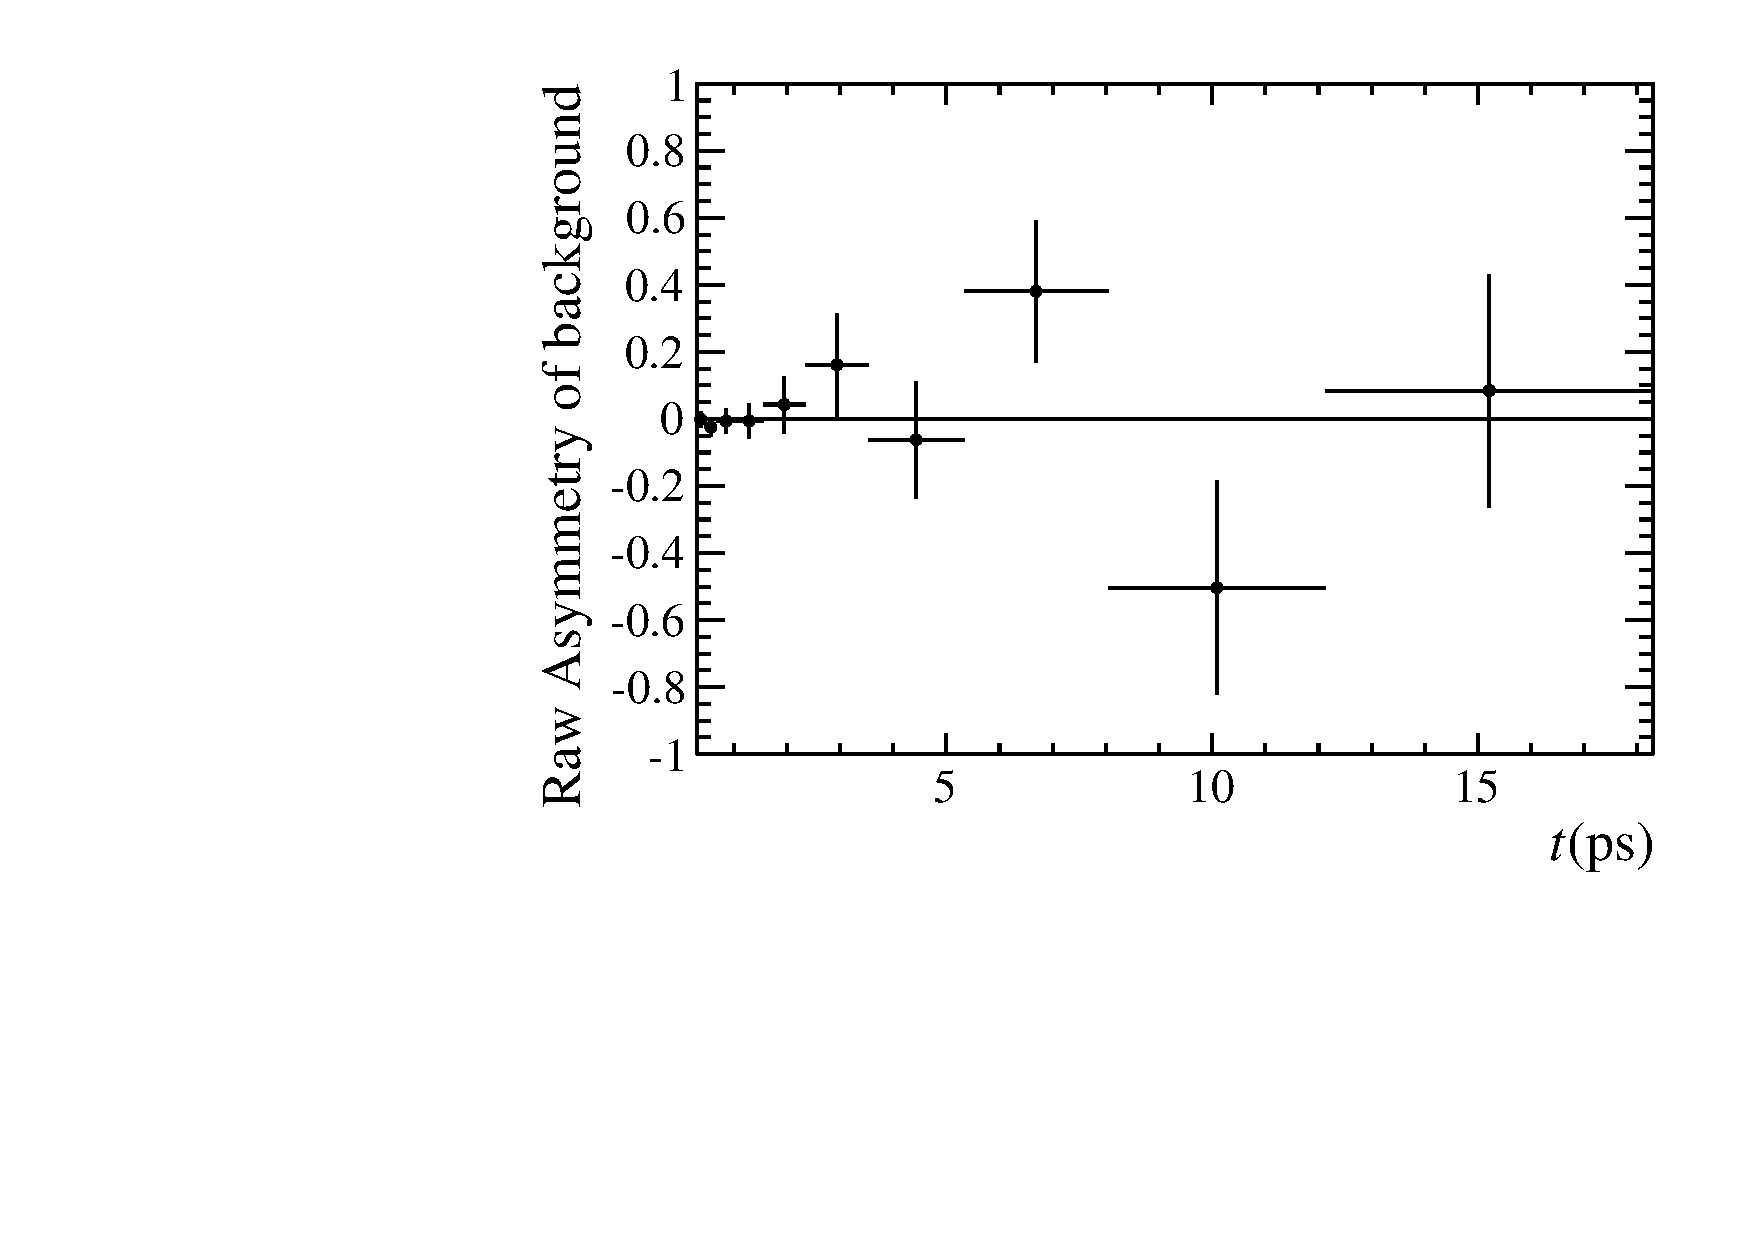
\includegraphics[width=0.49\textwidth]{06-Bd2JpsiKS/figs/BackgroundAsymmetryByHand_LL_OS_data.pdf}
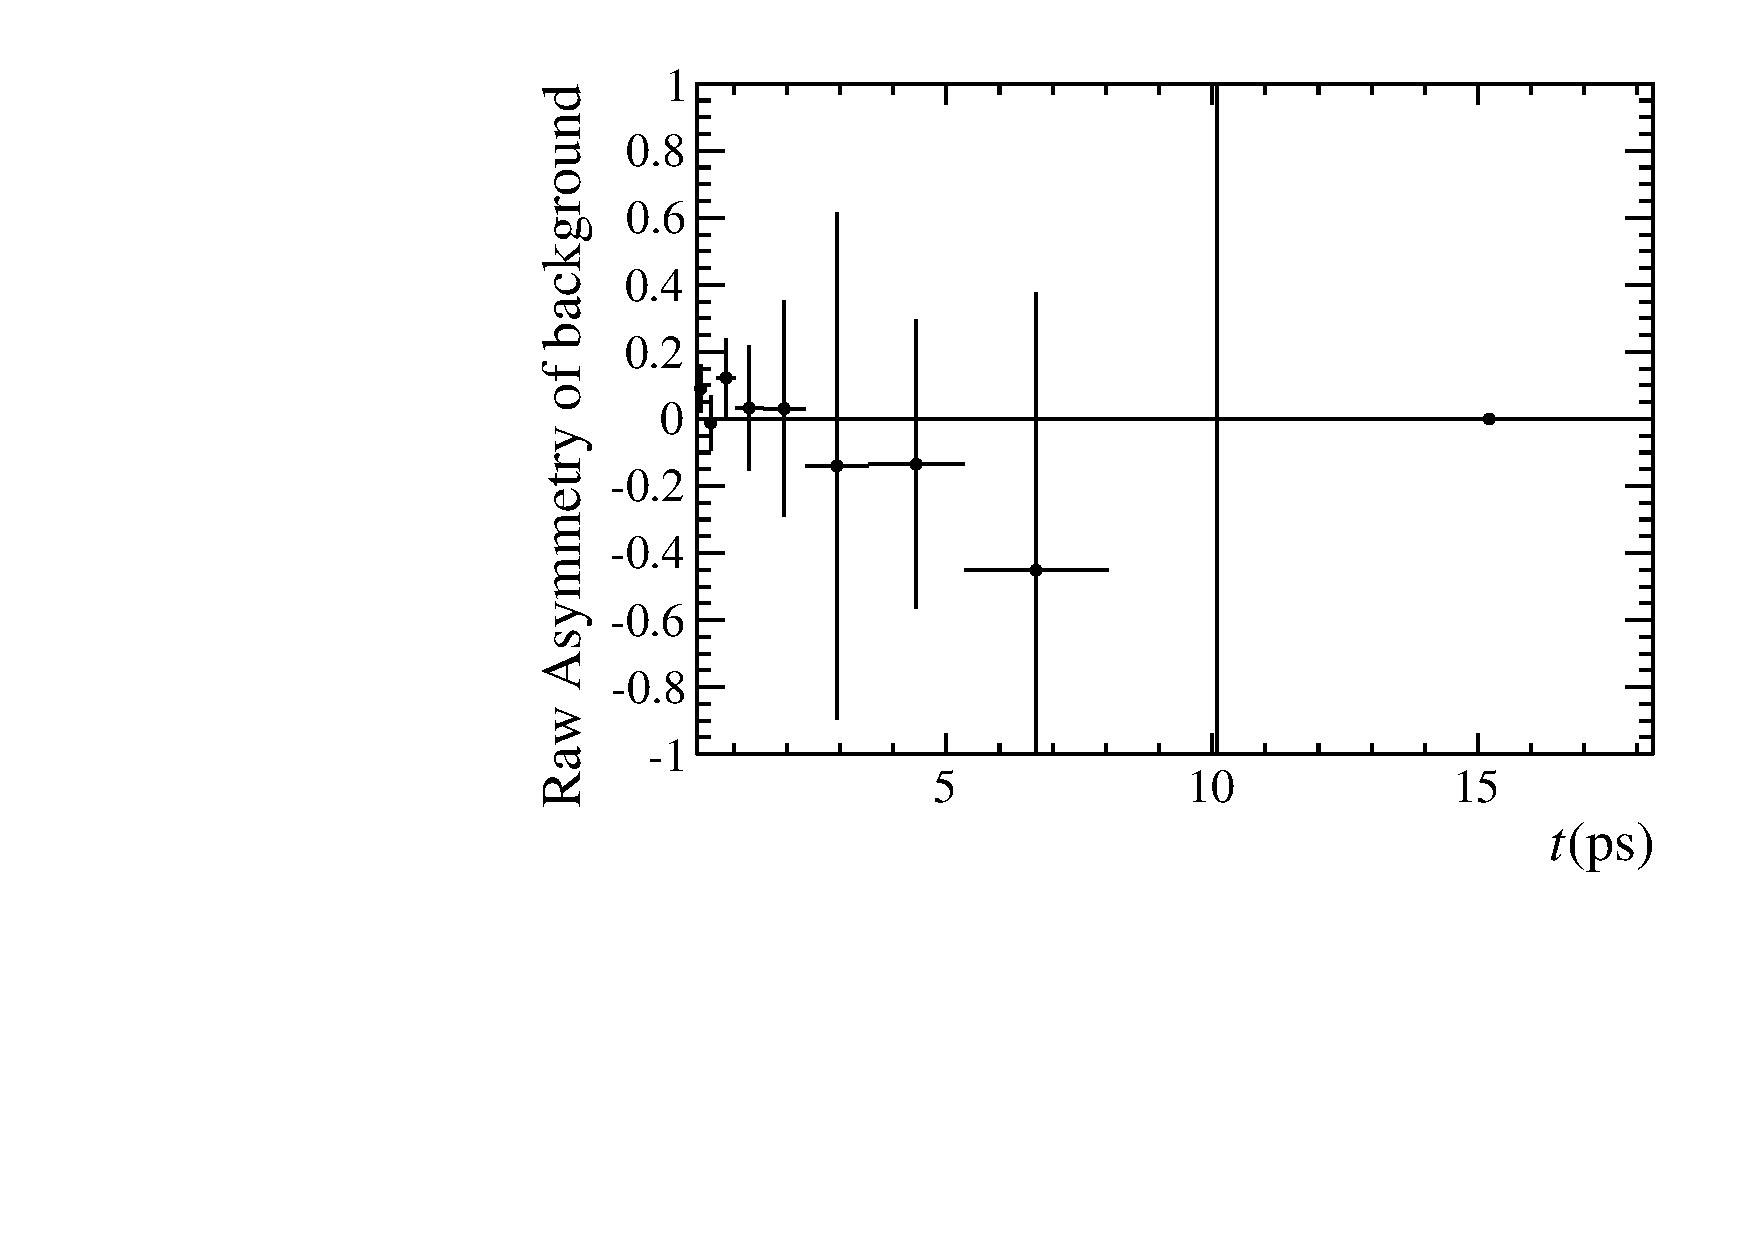
\includegraphics[width=0.49\textwidth]{06-Bd2JpsiKS/figs/BackgroundAsymmetryByHand_LL_SSPion_data.pdf}
\caption{Raw background asymmetry in sweighted data with logarithmic binning.
DD on top, LL on bottom plots. OS tagged candidates on the left, SS\pion tagged
candidates on the right side.}
\label{fig:background_asymmetry_sweighted}
\end{figure}
%
It's difficult to judge by eye if there is a significant oscillation. So,
\chisq-tests against the null-hypothesis, \ie a flat line at zero, are
performed and the corresponding $p$-values are calculated. The results are
\num{0.100} for DD OS, \num{0.437} for DD SS, \num{0.617} for DD SS, and
\num{0.969} for LL OS. None of the $p$-values is very low so the deviations
from zero can be explained with statistical fluctuations. The same procedure
(mass fit \to sWeights \to histograms of $\mathcal{A}_{\text{bkg}}$) is
performed with cocktail MC consisting of signal MC and background Toy MC.
Here, no asymmetry is generated for the background and the resulting
$p$-values are very similar to the ones for the nominal data sample. Finally,
an unbinned likelihood fit is performed to the sweighted background decay time
distribution using two/three exponentials with different pseudo-lifetimes and
allowing for tagging-dependent asymmetries in the PDF. All asymmetry
parameters are compatible with zero at a significance of two standard
deviations.

%!TEX root = ../main.tex

\section{Nominal fit (2 pages)}
\label{sec:bd2jpsiks:nominalfit}

A multi-dimensional fit to the distributions of the reconstructed mass $m$,
the decay time $t$ and its error prediction $\sigma_t$, the OS and SS\pion
tags and mistag probabilities is performed, mainly to extract the \CP
observables \SJpsiKS and \CJpsiKS. Thanks to the selection, which cleans up
the sample from other background contributions, besides the signal component
only the combinatorial background component needs to be parametrised.

The mass distribution, which enables the best discrimination of the two
components, is modelled by a modified Hypatia PDF~\cite{Santos:2013ky} and an
exponential function. All parameters are allowed to differ between the two
track type categories. The four tail parameters of the signal parametrisation
are taken from fits to simulated events.

The PDF describing the signal decay time distribution is basically given by
\cref{eq:cpviolation:simpledecayrates}. It is extended by taking into account
the production asymmetry and the experimental effects of mistagging.
Furthermore, it is convolved with the decay time resolution model presented in
\cref{sec:bd2jpsiks:decaytime:resolution} and multiplied by the time-dependent
efficiency correction for low and high decay times developed in
\cref{sec:bd2jpsiks:decaytime:acceptance}. The background decay time
distribution is parametrised with the sum of exponential functions. How many
of those give the best description in the various categories, in which the
whole data sample can be divided into, is determined in extensive studies
using sweighted background distributions (see
\cref{sec:bd2jpsiks:backgrounds}).

Lognormal distributions have been found to fit best when describing the decay
time error distributions. A combination of double and single lognormals with
some parameters being shared among the categories is used. Especially the
downstream and the long track distributions differ as can be seen in
\cref{fig:bd2jpsiks:nominalfit:time_error}.

\begin{figure}[htb]
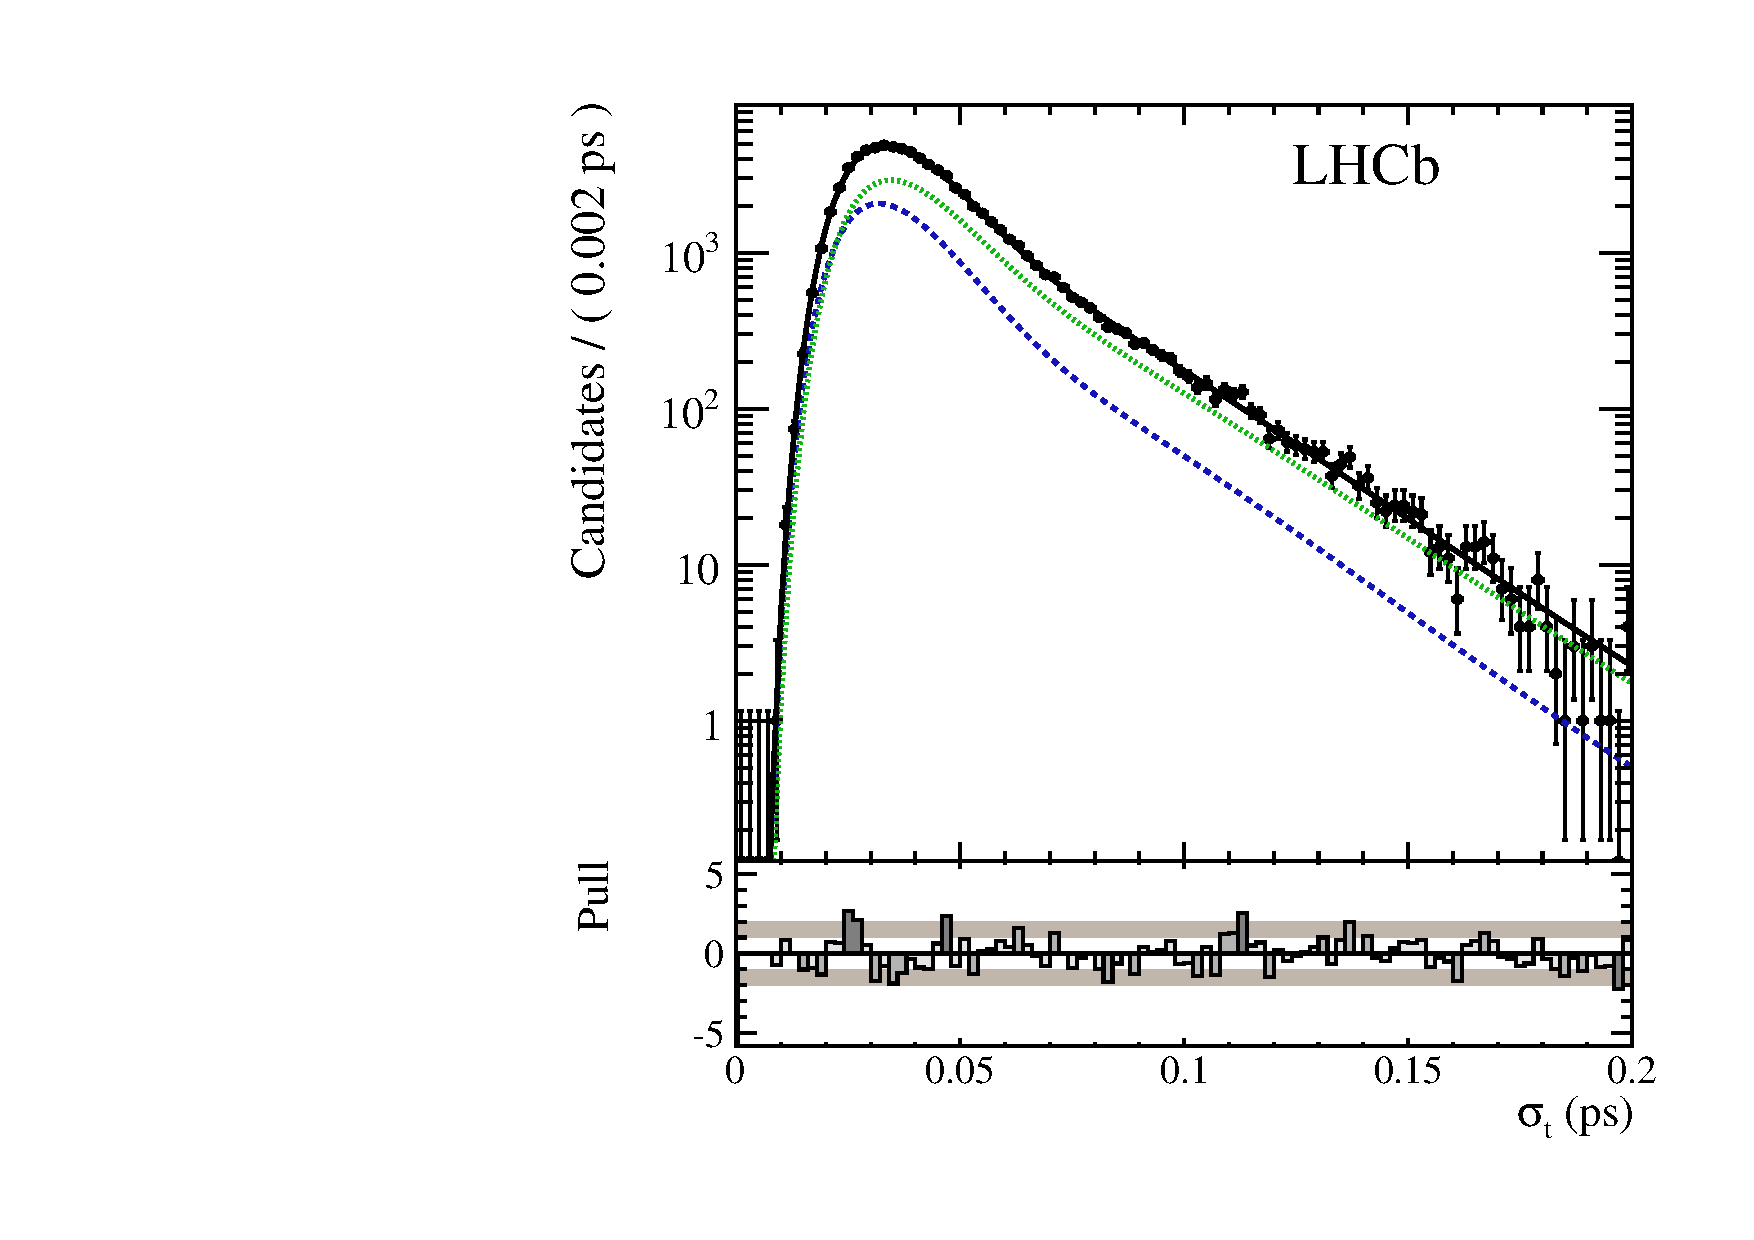
\includegraphics[width=0.49\textwidth]{06-Bd2JpsiKS/figs/obsTimeError_summed_pull_log_DD.pdf}
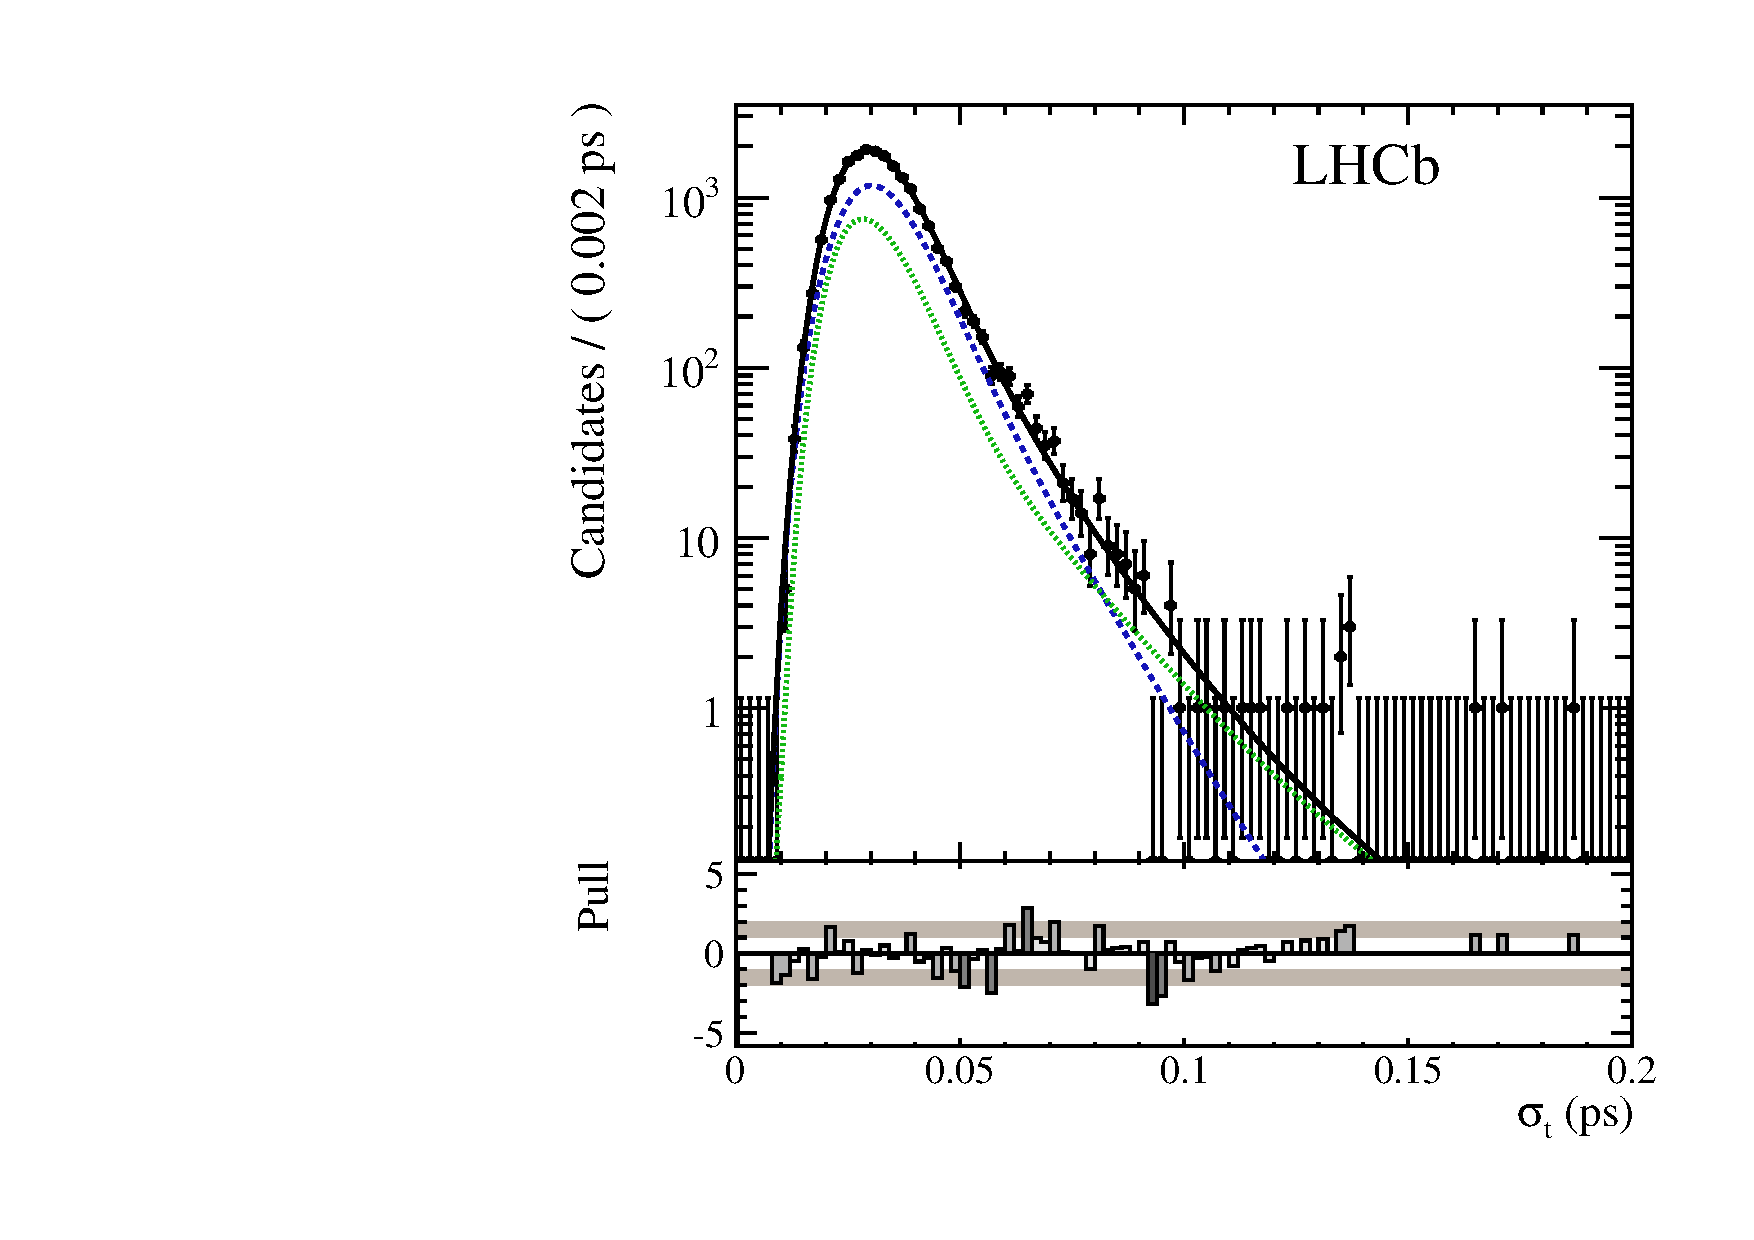
\includegraphics[width=0.49\textwidth]{06-Bd2JpsiKS/figs/obsTimeError_summed_pull_log_LL.pdf}
\caption{
Time error distributions of downstream (left) and long track (right). The solid black line
shows the fit projection, while the blue dashed (green dotted) line shows the
signal (background) component.}
\label{fig:bd2jpsiks:nominalfit:time_error}
\end{figure}
\todo{tikz version of time error plots}

The mistag distributions are described with cubic splines. The seven knots for
the SS\pion distribution, and similarly the 12 knots for the OS distribution,
are positioned where the shape visibly changes. It is checked that the two
mistag estimates are uncorrelated with each other and with the decay time, at
least within the available statistical precision. This allows to simply
multiply the corresponding PDFs.

In the fit 11 external input parameters are constrained within their
statistical uncertainties. These are the production asymmetries for
\SIlist{7;8}{\TeV}, for which the procedure is explained in more detail in
\cref{sec:b02dd:decaytimefit:constraints}, the oscillation frequency
\dmd~\cite{PDG2014} and the flavour tagging calibration parameters
(\cref{sec:dataanalysis:taggingcalibration:jpsixcalibration}).

To stabilize the fit the decay time resolution parameters, the spline
coefficients of the mistag parametrisation, the decay time error parameters
and all parameters included in the decay time acceptance model are fixed.
Thus, \num{72} floating parameters remain for the fit, of which \num{48} are
yields.

From the \num{41560} flavour-tagged \BdToJPsiKS decays the \CP observables are determined to be
\begin{align*}
  \SJpsiKS &=  \phantom{-}0.731 \, \pm 0.035 \, \text{(stat)} \pm 0.020 \, \text{(syst)}\,, \\
  \CJpsiKS &=  			- 0.038 \, \pm 0.032 \, \text{(stat)} \pm 0.005 \, \text{(syst)}\,,
\end{align*}
with a statistical correlation of \num{0.483}. In these results corrections of
\num{+0.002} for \SJpsiKS and \num{-0.005} for \CJpsiKS are included, which
account for \CP violation in $\Kz$--$\Kzb$ mixing and different nuclear
cross-sections in material between \Kz and
\Kzb~\cite{Fetscher:1996fa,*Ko:2010mk}.

The distributions of the invariant mass and the decay time are depicted in
\cref{fig:bd2jpsiks:nominalfit:mass_and_time}.

\begin{figure}[htb]
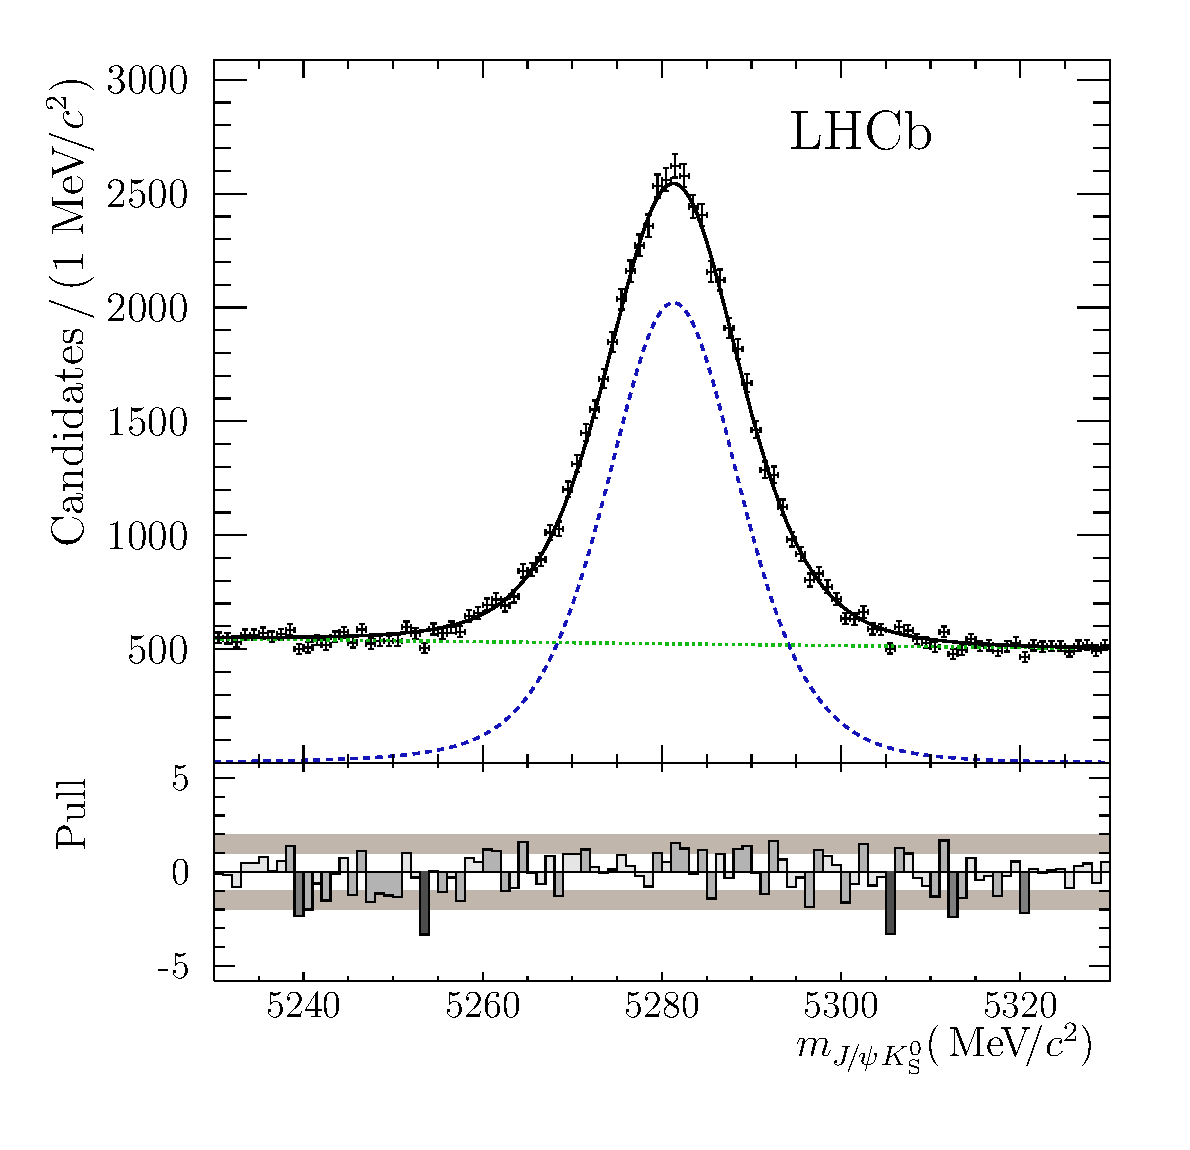
\includegraphics[width=0.49\textwidth]{06-Bd2JpsiKS/tikz/pdf/MassPulls_summed.pdf}
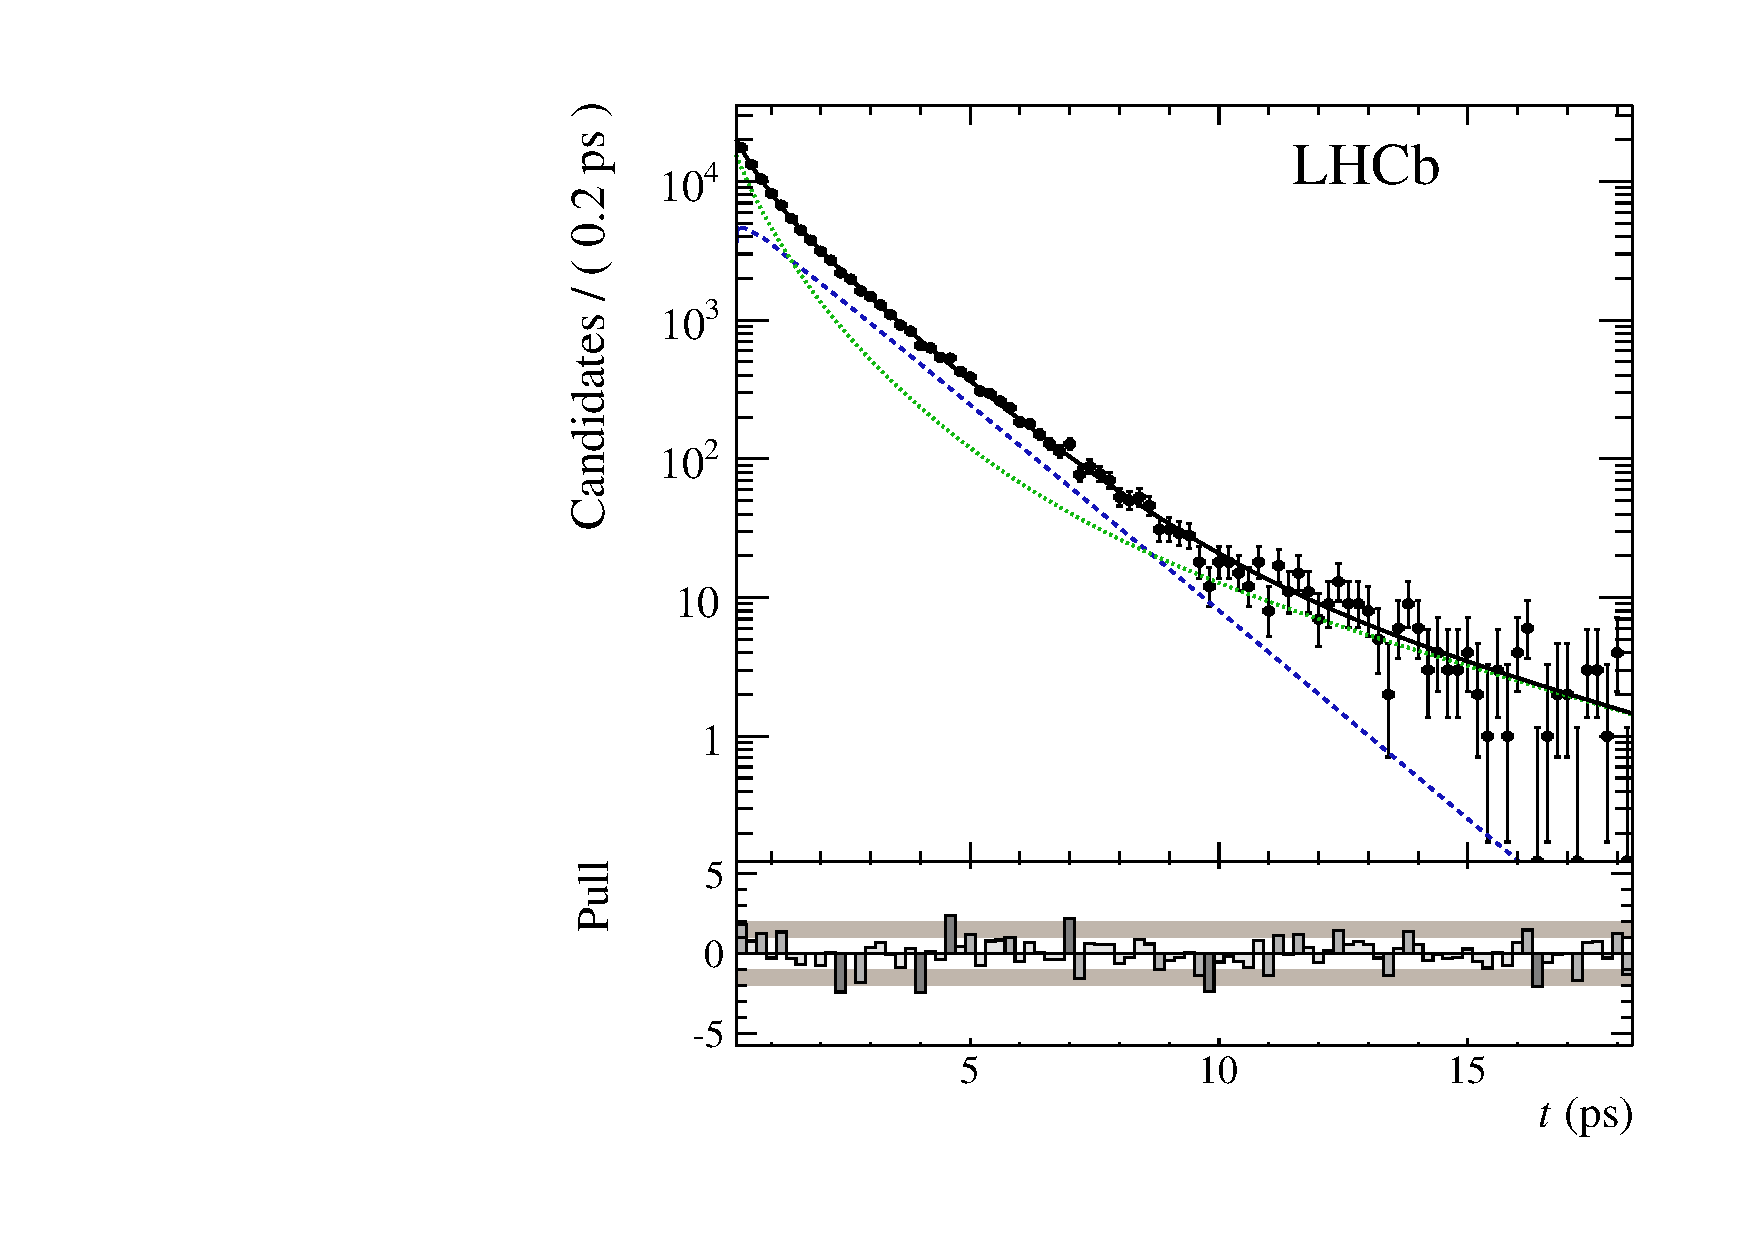
\includegraphics[width=0.49\textwidth]{06-Bd2JpsiKS/figs/obsTime_summed_pull_log.pdf}
\caption{
Invariant mass distribution (left) and decay time distribution (right). The solid black line
shows the fit projection, while the blue dashed (green dotted) line shows the
signal (background) component.}
\label{fig:bd2jpsiks:nominalfit:mass_and_time}
\end{figure}
\todo{decay time plot via tikz}

%!TEX root = ../main.tex

\section{Studies of systematic effects (5 pages)}
\label{sec:b02dd:systematics}

%============================================================================%
\subsection{Cross-checks}
\label{sec:systematics:xchecks}
To check for possible systematic effects, fits in different subsamples of the
nominal data set are performed. The cross-checks are performed for the two
tagging algorithms (OS vs. SS (not exclusive samples)), the two years of
data-taking (2011 vs. 2012) , combinations of those, the magnet polarities (Up
vs. Down), the two final states ($\KpipiKpipi$ vs. $\KKpiKpipi$) and for four
different slices of the BDT classifier for the $\KpipiKpipi$ final state.

\begin{figure}[thb]
\centering
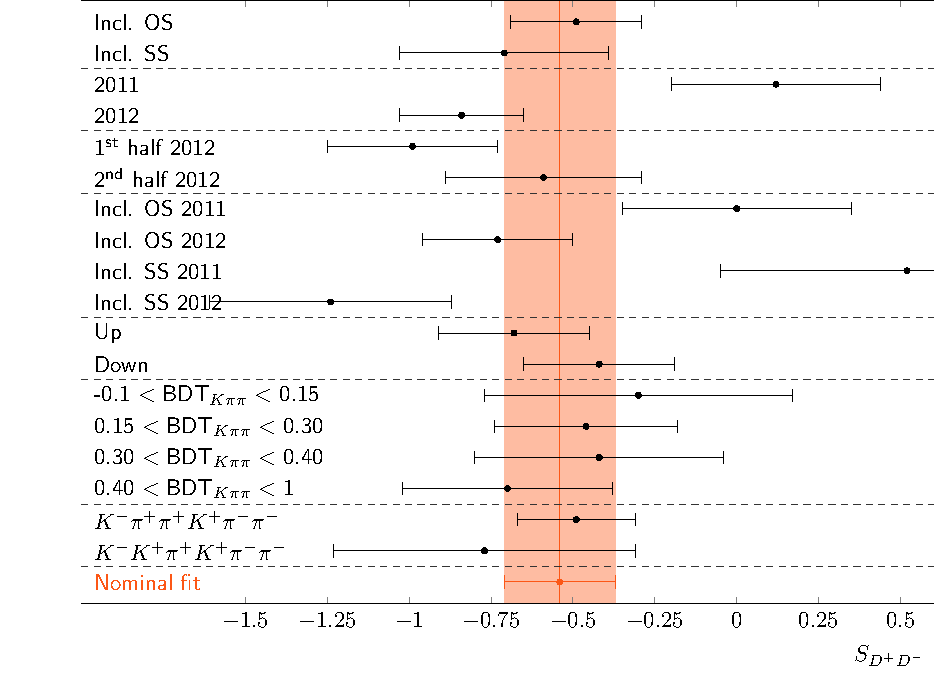
\includegraphics[width=0.9\textwidth]{07-B02DD/tikz/pdf/SComparison.pdf}
\caption{
Comparison of fit results of \SDD for fits on various subsamples.}
\label{fig:b02dd:systematics:xchecks:subsamples:s}
\end{figure}
\begin{figure}[thb]
\centering
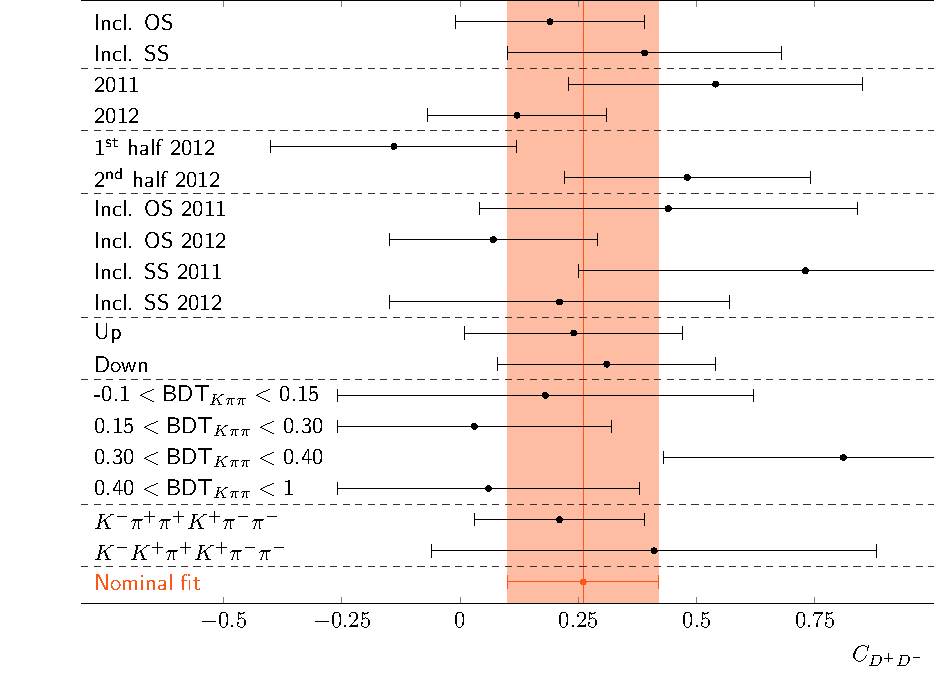
\includegraphics[width=0.9\textwidth]{07-B02DD/tikz/pdf/CComparison.pdf}
\caption{
Comparison of fit results of \CDD for fits on various subsamples.}
\label{fig:b02dd:systematics:xchecks:subsamples:c}
\end{figure}
The fit results in the various scenarios are illustrated in
\cref{fig:b02dd:systematics:xchecks:subsamples:s,fig:b02dd:systematics:xchecks:subsamples:c}.
While almost all splits show compatible results a rather large difference can
be observed between the 2011 and the 2012 subsample for $\SDD$. This is even
more pronounced when using only SS tagging. When determining the flavour
tagging calibration parameters separately for 2011 and 2012 data small
non-significant differences are observed but these can not explain the
different results of the $\CP$ observables. So the best explanation is that
the difference is due to a statistical fluctuation.

For the nominal fit the decay times and the decay time errors from the DTF are
used. The central values of the $\CP$ observables slightly change when using
the decay time (error) from the LVF, $\SDD = \num{-0.539}$ (LVF) vs.
\num{-0.541} (DTF) and $\CDD = \num{0.266}$ (LVF) vs. \num{0.263} (DTF). But
this difference is clearly below the statistical significance.

\FloatBarrier

%============================================================================%
\subsection{Decay Time Fit Bias}
\label{sec:b02dd:systematics:fitbias}

The likelihood fit itself might be biased. The nominal fit results for the
$\CP$ observables are used to generate \num{10000} pseudoexperiments. The pull
distributions in \cref{fig:b02dd:systematics:fitbias:pulls} show a very small
deviation of the mean value from zero.
%
\begin{figure}[htb]
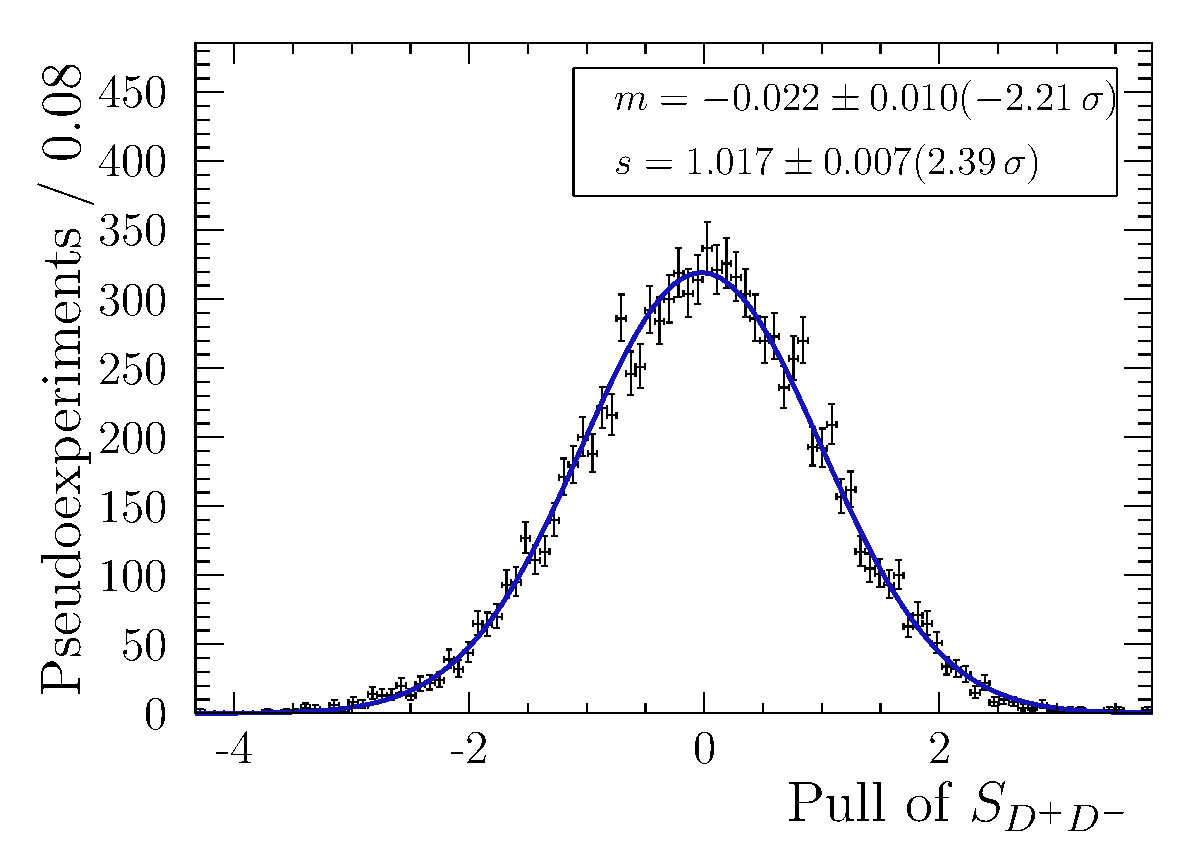
\includegraphics[width=0.49\textwidth]{07-B02DD/tikz/pdf/parSigTimeSin2b_pull_fitbias.pdf}
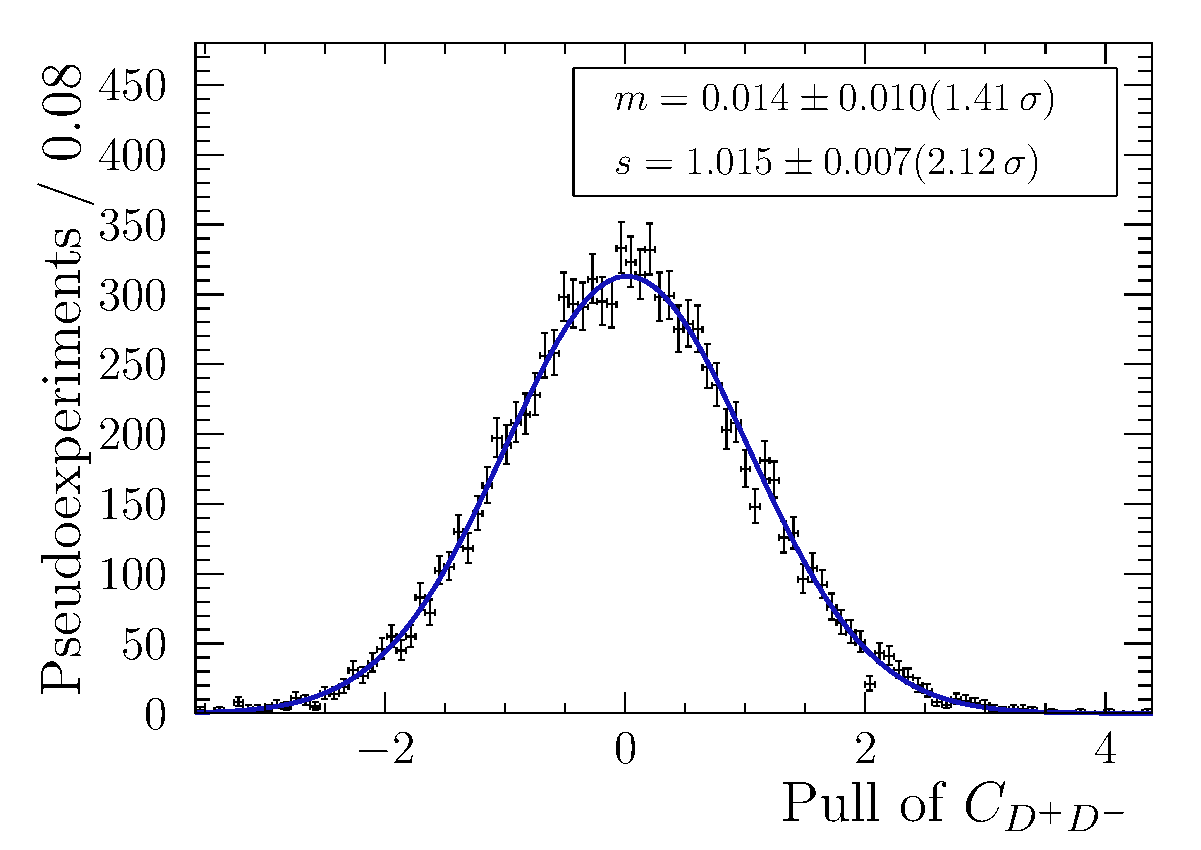
\includegraphics[width=0.49\textwidth]{07-B02DD/tikz/pdf/parSigTimeC_pull_fitbias.pdf}
\caption{Pull distributions of $\SDD$ and $\CDD$ for a study on the systematic
uncertainty due to the likelihood fitter.}
\label{fig:b02dd:systematics:fitbias:pulls}
\end{figure}
%
Multiplying it with the statistical uncertainty the systematic uncertainty is
calculated to be
\begin{align}
s_{\SDD}^{\textrm{fit}} = \num{0.004}\ , \qquad s_{\CDD}^{\textrm{fit}} = \num{0.0025}\ .
\end{align}
For all following studies of systematic uncertainties the residuals are
corrected for the decay time fit bias. Otherwise, even effects that are
actually not biasing would be misinterpreted due to the fit bias.

%============================================================================%
\subsection{Fit Model}
\label{sec:b02dd:systematics:fitmodel}
%!TEX root = ../main.tex

%----------------------------------------------------------------------------%
\subsubsection{Mass Model}
\label{sec:b02dd:systematics:massmodel}

Two different aspects of the mass model are studied regarding systematic
uncertainties: the impact of neglecting contributions and of mismodelling
components.

\paragraph{Neglected contributions}

If a neutral \piz or a photon is missed in the reconstruction the decay
\BToDstD, with \DstpToDpizero or \DstpToDgamma, can mimic the \BToDD decay. In
the rest frame of the \Dstarp resonance, the missing momentum of the \piz is
fixed, but it needs to be boosted when transferred into the rest frame of the
\PB meson. So, the reconstructed mass depends on the helicity angle of the
missing \piz. This leads to a double-horned structure approximately
\SI{140}{\MeVcc} below the nominal \PB mass (see Ref.~\cite{LHCb-ANA-2014-015}
for more details on the shape of this background). As the lower boundary on
the invariant $m_{\Dp\Dm}$ mass is set to \SI{5150}{\MeVcc} the \BdToDstD
contribution lies outside the mass range used for the fit. However, the
\BsToDstD contribution enters the fit region. But since the expected number of
\BsToDstD candidates is low, it is not included in the nominal mass model.
Another contribution that is neglected in the nominal mass fit model is
(partially) charmless background where at least one of the hadron triplets is
not originating from a \PD decay. The systematic uncertainty on the
determination of the \CP observables arising from neglecting these two
contributions is estimated using \num{1000} pseudoexperiments. Components for
\BsToDstD and for (partially) charmless background are included in the
generation but excluded from the fit procedure.

The shape of \BsToDstD is parametrised with two single Gaussian functions
centred around \SI{5150}{\MeVcc} and \SI{5200}{\MeVcc}. The (partially)
charmless background is modelled with a single Gaussian function. When
optimising the decay time significance cut it has been observed that the width
of the (partially) charmless background is approximately \SI{10}{\percent}
wider than the signal component. Therefore, a width of \SI{10}{\MeVcc} is
chosen. The mean is set to the same position as the \Bd signal. The \BsToDstD
component is generated without any tagging asymmetry, while for the (partially)
charmless background the worst case scenario of maximal \CP violation with the
opposite \CP eigenvalue ($S_f = \num{+1.0}$) is tested.

In studies of \BdToDstD decays~\cite{BToDstDthesis} a significant contribution
of \BsToDstD candidates is observed. The ratio between the two yields is
determined to be 1:20. Under the assumption that the efficiencies for \BToDD
and \BToDstD are the same the expected number of \BsToDstD candidates can be
calculated via
\begin{align}
	\text{N}_{\BsToDstD} = \frac{1}{20} \text{N}_{\BdToDD} \frac{\mathcal{B}(\BdToDstD) \mathcal{B}(\Dstarp \!\to \Dp (\piz || \gamma))}{\mathcal{B}(\BdToDD)} \,.
\end{align}
Using the world averages for the branching ratios~\cite{PDG2016} the number of
candidates to be generated in the pseudoexperiments is estimated to be
N(\BsToDstD) = \num{66\pm9}.

To determine how many (partially) charmless background candidates need to be
generated the $D$ mass window is widened to $\SI{\pm40}{\MeVcc}$ and the
nominal $D$ mass window of $\SI{\pm25}{\MeVcc}$ is vetoed for one or for both
$D$ candidates. Fits to the invariant $B$ mass without the $D$ mass constraint
are performed in the various scenarios. % yielding
% $\num{0.0\pm2.6}\,\mbox{\Bd\!\to\KpipiKpipi}$ candidates,
% $\num{0.0\pm9.2}\,\mbox{\Bd\!\to\KKpiKpipi}$ candidates,
% $\num{0.0\pm4.9}\,\mbox{\Bd\!\to\D(\Kpipi)\Kpipi}$ candidates,
% $\num{0.0\pm3.3}\,\mbox{\Bd\!\to\D(\KKpi)\Kpipi}$ candidates, and
% $\num{17.2\pm11.2}\,\mbox{\Bd\!\to\D(\Kpipi)\KKpi}$ candidates.
%
The fitted yields, which are constrained to positive values, are scaled to
account for the applied $D$ mass window. The total amount of residual
contamination ($\Bz\!\to\PD hhh$ or $\Bz\!\to hhhhhh$ decays) surviving the
\BdToDD selection is found to be $\num{28.7\pm19.5}$ candidates for the
$\KKpiKpipi$ final state and $\num{0.0\pm27.8}$ candidates for the
$\KpipiKpipi$ final state. For the pseudoexperiments the number of (partially)
charmless background is drawn from Gaussian distributions using these values
for mean and width. When the outcome is negative the procedure is repeated,
until a positive yield is drawn.

The systematic uncertainties on \SDD and \CDD are calculated as the product of
the bias on the mean parameter of the pull distributions and the statistical
uncertainty:
\begin{align*}
s_{\SDD}^{\text{mass,1}} = \num{0.05}\ , \qquad s_{\CDD}^{\text{mass,1}} = \num{0.013}\,.
\end{align*}

\paragraph{Mismodelling of mass components}

The BDT is trained with MC samples that are known to not perfectly model the
PID information. As a result the BDT classifier distributions of
background-subtracted data and MC show a quite big discrepancy. Some shape
parameters are estimated on MC samples and might be distorted by the data/MC
differences. Therefore, different alternative mass parametrisations are tested
against the nominal model: the component of the \BdToDD signal (and of the
\BsToDD background) is parametrised with a single Gaussian function; the
combinatorial background is described with a second order Chebyshev polynomial
of first kind; the tail parameters of \BToDsD are once extracted from the MC
sample without applying the BDT and once applying a tight cut on the BDT
classifier. The mass fit is performed with these new models, sWeights are
calculated for each approach, and the decay time fit is performed. The results
of the \CP observables are then compared with the nominal central values. The
largest deviations for \SDD and \CDD are
\begin{align*}
s_{\SDD}^{\text{mass,2}} = \num{0.004}\ , \qquad s_{\CDD}^{\text{mass,2}} = \num{0.006}\,.
\end{align*}

%----------------------------------------------------------------------------%
\subsubsection{Correlation between decay time and mistags}
\label{sec:b02dd:systematics:correlation_mistag_time}

The correlation between the decay time distribution and the per-event mistags
is studied by calculating the linear Pearson correlation coefficient
$\rho(\eta,t)$. The significance of the correlation value, \ie
\SI{95}{\percent} confidence level interval, is determined using the
bootstrapping method (\cref{sec:dataanalysis:bootstrapping}) with \num{10000}
repetitions. The correlation coefficients are found to be small. The profile
histogram of the OS tagging combination, which shows the average \etaos value
as a function of the decay time, is flat within statistics. For the SS tagging
combination the profile histogram slowly increases with decay time. This can
be confirmed by analysing the larger signal MC sample (see
\cref{fig:b02dd:systematics:correlation_mistag_time:etass_time_profile_MC}).
\begin{figure}[htb]
\centering
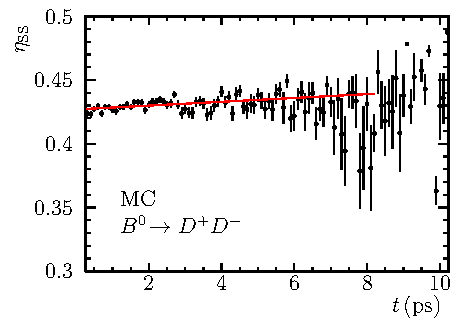
\includegraphics[width=0.6\textwidth]{07-B02DD/tikz/pdf/Profile_DecayTime_SS.pdf}
\caption{Profile histogram for the decay time dependence on $\etass$ for
signal MC. The black data points represent the mean value of $\etass$ and its
uncertainty for each bin in $t$. The red curve is the fitted linear function.}
\label{fig:b02dd:systematics:correlation_mistag_time:etass_time_profile_MC}
\end{figure}
Performing a $\chisq$ fit in the decay time range \SIrange{0.25}{8.25}{\ps}
with the linear function
\begin{align}
  \etass = a_{\etass,t} t + b_{\etass,t}
  \label{eq:tagging:correlation_mistag_time}
\end{align}
yields a slope of $a_{\etass,t} = \SI{1.50\pm0.27}{\invns}$. Although this is
a significant deviation from zero, the correlation is not taken into account in
the nominal fit model. Instead, a study on the systematic uncertainty from
neglecting this effect is performed. In \num{1000} pseudoexperiments the SS
mistag is generated using a Gaussian distribution whose mean is drawn from the
linear function defined in \cref{eq:tagging:correlation_mistag_time} thereby
introducing the correlation with the decay time. In the subsequent fit the
correlation is again ignored. This leads to systematic uncertainties of
\begin{align*}
s_{\SDD}^{\text{corr}} = \num{0.0007}\ , \qquad s_{\CDD}^{\text{corr}} = \num{0.007}\,.
\end{align*}

%----------------------------------------------------------------------------%
\subsubsection{Decay Time Resolution Model}
\label{sec:systematics:decaytimeresolution}

As calculated in \cref{sec:b02dd:decaytimefit:resolution} even an
underestimation of the decay time resolution by \SI{15}{\percent} has only a
minor effect on the resolution related dilution. Nevertheless, \num{1000}
pseudoexperiments are performed, in which the scale factors and the offset
parameters ($b_i$ and $c_i$ from \cref{tab:b02dd:decaytimefit:resolution}) are
enlarged by \SI{15}{\percent} in the generation and fixed to their nominal
values in the fit. Additionally, the mean parameter of the Gaussians is set to
the value obtained in the MC study for the generation and, like in the nominal
setup, fixed to zero in the fit. The systematic uncertainties are calculated
as the product of the biases on the mean parameter and the statistical
uncertainty to be
\begin{align*}
s_{\SDD}^{\text{res}} = \num{0.0020}\ , \qquad s_{\CDD}^{\text{res}} = \num{0.0023}\,.
\end{align*}

%----------------------------------------------------------------------------%
\subsubsection{Decay Time Acceptance Model}
\label{sec:systematics:decaytimeacceptance}

On signal MC the decay time acceptance is determined separately for the two
final states (see \cref{fig:b02dd:decaytimefit:acceptance_MC}). Small
differences are observed. As the low statistics in the \KKpiKpipi final state
on data does not allow for an individual spline model, a study is performed to
estimate a possible systematic uncertainty from neglecting this difference. In
\num{1000} pseudoexperiments the decay time distribution is generated using
the histograms of the true decay time acceptance from signal MC, split by
final state, and fitted with the spline acceptance as done in the nominal fit.
The use of the histograms with \num{100} bins should also cover uncertainties
from the choice of the number and position of the knots. The pull between the
fit results and the generation values is calculated. The systematic
uncertainty due to the decay time acceptance model is calculated as the
product of the shift in the pull distribution and the statistical uncertainty
of the nominal fit:
\begin{align*}
s_{\SDD}^{\textrm{acc}} = \num{0.007}\ , \qquad s_{\CDD}^{\textrm{acc}} = \num{0.0027}\,.
\end{align*}


%============================================================================%
\subsection{Further Studies}
\label{sec:b02dd:systematics:others}
%!TEX root = ../main.tex

%----------------------------------------------------------------------------%
\subsubsection[\texorpdfstring{$z$}{z}-scale]{\texorpdfstring{$\boldsymbol{z}$}{z}-scale}
\label{sec:b02dd:systematics:z_scale}

The decay times are determined by measuring the distance between PV and decay
vertex. So, any uncertainty on the positioning of detector elements
(especially the VELO modules) leads to biased decay times. Due to the high
boosting the main contribution to the flight distance is in $z$ direction. The
scale uncertainty in $z$ direction has been estimated to be
$\sigma_{z\text{-scale}} = \SI{0.022}{\percent}$~\cite{LHCb-ANA-2011-055}. The
influence on the measurement of the \CP observables is studied by performing
\num{1000} pseudoexperiments. For each pseudoexperiment a value for the uncertainty
on the $z$-scale is drawn from a Gaussian distribution around zero of width
$\sigma_{z\text{-scale}}$. The sum of \SI{50}{\fs} and the product of this
value with the decay time is used as width of the Gaussian function modelling
the decay time resolution in the generation. In the fit the width is set to
\SI{50}{\fs}. The product of the bias from the pull distributions of the
pseudoexperiments and the nominal statistical uncertainty is taken as
systematic uncertainty:
\begin{align*}
s_{\SDD}^{z\text{-scale}} = \num{0.0031}\ , \qquad s_{\CDD}^{z\text{-scale}} = \num{0.0028}\,.
\end{align*}

%----------------------------------------------------------------------------%
\subsubsection{Production Asymmetry}
\label{sec:b02dd:systematics:production_asymmetry}

The systematic uncertainty on the production asymmetry \prodasym{11} is
studied using \num{1000} pseudoexperiments. The nominal value is used in the
generation and the procedure described in Ref.~\cite{Karbach:1490463} is
applied in the fit: Before fitting the data sample the mean of the Gaussian
constraint for \prodasym{11} is shifted by one systematic uncertainty. The
resulting Gaussian distribution is used to draw a new value for the mean.
Then, the new Gaussian distribution is used to constrain \prodasym{11} in the
fit. Both shifts, upwards and downwards, are tested and the larger deviation
is taken as systematic uncertainty:
%
\begin{align*}
s_{\SDD}^{\prodasym{}} = \num{0.0015}\ , \qquad s_{\CDD}^{\prodasym{}} = \num{0.004}\,.
\end{align*}
%
For the production asymmetry difference $\Delta\prodasym{}$ the systematic
uncertainty is already included in the Gaussian constraint of the nominal fit.

%----------------------------------------------------------------------------%
\subsubsection{Decay Width Difference \texorpdfstring{\DGd}{Delta Gamma\_d}}
\label{sec:b02dd:systematics:deltagammad}

The decay width difference \DGd is expected to be very small and therefore
fixed to zero in the nominal fit. But experimentally it has a relatively large
uncertainty. This is taken into account by performing \num{1000}
pseudoexperiments where the current statistical precision $\sigma(\DGd) =
\SI{\pm0.007}{\invps}$~\cite{HFAG} is used in the generation of the data
samples while it is, like in the nominal model, neglected in the fit. The mean
parameters of the pull distributions are converted into systematic
uncertainties of
\begin{align*}
s_{\SDD}^{\DGd} = \num{0.014}\ , \qquad s_{\CDD}^{\DGd} = \num{0.0021}\,.
\end{align*}

%----------------------------------------------------------------------------%
\subsubsection{\texorpdfstring{$\Bz$}{B0} Mass Difference \texorpdfstring{\dmd}{Delta m\_d}}
\label{sec:b02dd:systematics:deltamd}

The systematic uncertainty on the world average of \dmd
($\SI{\pm0.002}{\hbar\invps}$~\cite{HFAG}) is not covered by the Gaussian constraint that
is used in the nominal fit. Instead, it is analysed using \num{1000}
pseudoexperiments. In the generation the nominal model is used. Before
performing the fit the mean of the Gaussian distribution (its width is the
statistical precision of the world average) is shifted by one systematic
uncertainty (once up and once down) and a new value is drawn from the
distribution. This new constraint is then used in the minimisation. Looking at
the resulting pull distributions systematic uncertainties of
\begin{align*}
s_{\SDD}^{\dmd} = \num{0.0025}\ , \qquad s_{\CDD}^{\dmd} = \num{0.006}\,,
\end{align*}
are assigned.


% \FloatBarrier
%============================================================================%
\subsection{Total Systematic Uncertainty}
\label{sec:b02dd:systematics:total}

The systematic uncertainties are summarised in
\cref{tab:b02dd:systematics:total}. The full systematic uncertainty is
calculated by summing the individual uncertainties in quadrature.
%
\begin{table}[!htb]
\caption{Systematic uncertainties on the $\CP$ observables $\SDD$ and $\CDD$.}
\label{tab:b02dd:systematics:total}
  \centering
    \begin{tabular}{lSS}
      \toprule
      Origin & {\param{\sigma}{}{$\SDD$}} & {\param{\sigma}{}{$\CDD$}}    \\
      \midrule
      Neglecting components in mass model     &  0.05    & 0.013  \\
      $\DGd$                                  &  0.014   & 0.0021 \\
      Decay time acceptance                   &  0.007   & 0.0027 \\
      Correlation between mass and decay time &  0.0007  & 0.007  \\
      Parametrisation of PDFs in mass model   &  0.004   & 0.006  \\
      $\dmd$                                  &  0.0025  & 0.006  \\
      Fit bias                                &  0.004   & 0.0025 \\
      Production asymmetry                    &  0.0015  & 0.004  \\
      $z$-scale                               &  0.0031  & 0.0028 \\
      Decay time resolution                   &  0.0020  & 0.0023 \\
      \midrule
      Sum                                     &  0.05    & 0.018  \\
      \bottomrule
    \end{tabular}
\end{table}

%!TEX root = ../main.tex

\chapter[Measurement of \texorpdfstring{$\CP$}{CP} Violation in \texorpdfstring{$\BdToDD$}{Bd2DD} Decays]{Measurement of \texorpdfstring{$\CP$}{CP} Violation in \texorpdfstring{$\BdToDD$}{Bd2DD} Decays}
\label{sec:b02dd}

In this chapter the analysis of \BdToDD decays with the goal to determine the
observables \SDD and \CDD, which describe the \CP violation in this decay
mode, is presented~\cite{LHCb-PAPER-2016-037}. After a description of the
selection (see \cref{sec:b02dd:selection}) the fit of the invariant mass
distribution, performed to extract signal sWeights, is described (see
\cref{sec:b02dd:massfit}). This is followed by a summary of the decay time fit
(see \cref{sec:b02dd:decaytimefit}). The chapter is concluded with a
presentation of the studies on systematic uncertainties (see
\cref{sec:b02dd:systematics}). The new OS combination including the OS charm
tagger and the SS combination of SS\pion and SS\proton tagger are used to
determine the flavour tag of the \Bd mesons. The calibration of these
flavour-tagging algorithms using \BdToDsD decays (see
\cref{sec:dataanalysis:taggingcalibration:dsdcalibration}) is the only part
not performed by myself but by collaborators from Milano.

%!TEX root = ../main.tex

\section{Selection (5 pages)}
\label{sec:b02dd:selection}

The amount of background in \BdToDD is too high to perform a significant
measurement of \CP violation without any selection. The selection is divided
into three parts: a preselection with many high signal efficiency
requirements, a dedicated treatment of mis-identified backgrounds and a
multivariate analysis to further reduce combinatorial background.

\subsection{Preselection}
\label{sec:b02dd:selection:cuts}

Only events that have been triggered by a topological trigger line or by the
inclusive $\phi$ line and that in total contain less than \num{500} long
tracks are considered. All candidate kaon and pion tracks have to be long
tracks and have to satisfy quality criteria. Lower limits on the momentum ($p
> \SI{1}{\GeVc}$) and on the transverse momentum ($\pT > \SI{100}{\MeVc}$) are
required. The candidates should be inconsistent with originating from the PV
and the particle identification (PID) system needs to classify them as pions
or kaons with only a small probability to be a ghost.

Of all the possible combinations of three charged hadron tracks forming a
$\Dp$ meson candidate only the two possibilities \DToKpipi and \DToKKpi are
used. The vertex needs to be significantly displaced from all PVs in the event
and the distance of the closest approach between all pairs of particles
forming the vertex has to be below \SI{0.5}{\mm}. The scalar sum of the \pT
has to exceed \SI{1800}{\MeVc} and the combined invariant mass has to be in
the range \SI{\pm25}{\MeVcc} around the nominal \Dp mass~\cite{PDG2014}. The
tightened mass window as well as requiring that the \chisq of the flight
distance of each $\Dpm$ meson with respect to the $\Bd$ decay vertex has to be
larger than \num{2} reduces the amount of (partially) charmless contributions.
On top of that, a cut on the decay time significance of the $\Dpm$ mesons,
defined as their decay time with respect to the $\Bz$ decay vertex divided by
the corresponding uncertainty, is supposed to further suppress the (partially)
charmless contributions. The optimal cut value is estimated under the
assumption that a very tight cut leaves only candidates with resonant $\Dpm$
mesons. Gradually loosening the cut the value can be found where the product
of the \Bd signal yield, extracted from a fit on data, and the signal
efficiency, determined on MC, exceeds the estimation from the initial tight
cut scenario. If both $\Dpm$ mesons are reconstructed via \DToKpipi decays the
decay time significance has to be greater than \num{0}. It needs to be greater
than \num{3} if one of the $\Dpm$ mesons is reconstructed in the \KKpi and the
other in the \Kpipi final state. Although in this case the final states
of the \Dpm mesons differ the same cut is applied to both \Dpm mesons as on
signal MC the comparison of the distributions of the decay time significance
shows a good agreement between \DToKpipi and \DToKKpi decays.

The vertex formed by a pair of oppositely charged $\Dpm$ candidates needs to
be of good quality. The scalar sum of the $\pT$ of the $\Dpm$ mesons must
exceed $\SI{5}{\GeVc}$. In the stripping a BDT to select $\Bd$ candidates is
applied. The BDT is based on the \pT and the flight distance \chisq of the \Bz
as well as on the sum of the \Bz and both \PD vertex \chisq's divided by the
sum of the degrees of freedom of these vertex fits. Moreover, the \Bd
candidates are required to have $p > \SI{10}{\GeVc}$ and to have
$\chisqip<\num{25}$, where $\chisqip$ is defined as the difference in the
vertex fit $\chi^2$ of the associated PV with and without the $B^0$ candidate.

The reconstructed decay time $t$ of the \Bd candidate is determined from a
DTF, in which the \Bd production vertex is constrained to the position of the
associated PV. Only candidates with decay times in the range
\SIrange{0.25}{10.25}{\ps} are kept. The invariant mass $m_{\Dp\Dm}$ of the
$\Bd$ candidate has to be in the range \SIrange{5150}{5500}{\MeVcc}. It is
calculated from a DTF, in which the invariant masses of $\Kpipi$ and $\KKpi$
are additionally constrained to the known $\Dp$ mass. It is required that
these fits have converged. Further outliers are removed by requiring that the
uncertainty on the invariant mass and on the decay time has to be below
\SI{30}{\MeVcc} and \SI{0.2}{\ps}, respectively, and that the absolute value
of the $z$ coordinate of the PV is smaller than \SI{250}{\milli\meter}.

The signal efficiency of the preselection for the final state with two kaons
is $\SI{82}{\percent}$ at a background rejection of $\SI{94}{\percent}$. For
the final state with three kaons the signal efficiency is
$\SI{67.5}{\percent}$ at a background rejection of $\SI{98}{\percent}$.

\subsection{Vetoes}
\label{sec:b02dd:selection:vetoes}

A $K\rightarrow\pi$ mis-ID can lead to background contributions from
$\DspToKKpi$, which predominantly proceeds through $\DsTophipi$. To reduce
these $\Dsp$ contributions the kaon mass hypothesis is assigned to the pion
with the higher transverse momentum of $\DpToKpipi$ candidates. The candidate
is rejected if the invariant mass of the hypothetical kaon pair is compatible
with the $\phi$ mass of $M_{\phi} = \SI{1019.461}{\MeVcc}$~\cite{PDG2014}
within $\pm\SI{10}{\MeVcc}$ or if the invariant mass $m(\Km\Kp\pip)$ is
compatible with the \Dsp mass of $M_{\Dsp} =
\SI{1968.30}{\MeVcc}$~\cite{PDG2014} within $\pm\SI{25}{\MeVcc}$ and the pion
with the higher \pT (the one that the kaon mass hypothesis is assigned to) has
a larger $\texttt{ProbNN}K$ than $\texttt{ProbNN}\pion$ probability. When
assigning the kaon mass hypothesis to the pion with the lower \pT no vetoes
are applied as no resonant structures at the $\phi$ or the $\Dsp$ mass are
found.

To reduce $p\rightarrow\pi$ mis-ID the proton mass hypothesis is assigned to
the pion with the higher \pT of $\DpToKpipi$ candidates. The candidate is
rejected if the invariant mass of the $\kaon\proton\pion$ combination is
compatible with the \Lc mass of $M_{\Lc} =
\SI{2286.46}{\MeVcc}$~\cite{PDG2014} within $\pm\SI{25}{\MeVcc}$ and the
proton probability $\texttt{ProbNN}p$ of the pion with the higher \pT is
larger than $\texttt{ProbNN}\pion$.

\subsection{Multivariate analysis}
\label{sec:b02dd:selection:mva}

\subsubsection*{BDT training}
\label{sec:b02dd:selection:mva:training}

To further suppress combinatorial background a Boosted Decision Tree
(BDT)~\cite{Breiman,Roe} based on the implementation in
TMVA~\cite{Hocker:2007ht} is trained using a signal MC sample and the upper
mass sideband with $m_{\Dp\Dm} > \SI{5500}{\MeVcc}$. The training is performed
on half of these samples while the other half is used to test the BDT
performance. The selection steps described above, are applied before the
training.

Two BDTs separated by the number of kaons in the \Bd final state are trained.
The importance of the \num{21} input variables to the training differs, which
is considered by their order in \cref{tab:b02dd:selection:mva:inputs}.
%
\begin{table}[!htb]
\centering
\caption{List of input variables used in the training of the BDTs.}
\begin{tabular}{ll}
 \toprule
  BDT for \KpipiKpipi                          &  BDT for \KKpiKpipi                           \\
\midrule
  min(\Dpm $\tau$ significance)                &  PID ratio of \Kpm                            \\
  $B$ direction angle                          &  $B$ direction angle                          \\
  $\log($DTF $\chi^2$/ndof$)$                  &  PID ratio of \Kp                             \\
  PID ratio of \Km                             &  $\log($DTF $\chi^2$/ndof$)$                  \\
  PID ratio of \Kp                             &  PID ratio of \Km                             \\
  min \pT of \Kpm                              &  min(\Dpm $\tau$ significance)                \\
  $\log(B$ impact parameter $\chi^2)$          &  $\log($min($h$ Velo $\chi^2$/ndof)$)$        \\
  $\log($min(\pipm Velo $\chi^2$/ndof)$)$      &  \pT of \Kpm                                  \\
  \pT of \pim with lower \pT                   &  $\log($min(\Kpm T-track $\chi^2$/ndof)$)$    \\
  $\log($min(\Kpm T-track $\chi^2$/ndof)$)$    &  $\log(B$ impact parameter $\chi^2)$          \\
  $\log($min(\pipm T-track $\chi^2$/ndof)$)$   &  PID ratio of \pipm with lower \pT            \\
  PID ratio of \pim with higher \pT            &  $\log($min($h$ VELO-T-Match $\chi^2$)$)$     \\
  \pT of \pip with lower \pT                   &  $\log($min(\Kpm Velo $\chi^2$/ndof)$)$       \\
  PID ratio of \pim with lower \pT             &  PID ratio of single \pipm                    \\
  PID ratio of \pip with higher \pT            &  \pT of \pipm with higher \pT                 \\
  \pT of \pip with higher \pT                  &  $\log($min($h$ T-track $\chi^2$/ndof)$)$     \\
  PID ratio of \pip with lower \pT             &  \pT of \pipm with lower \pT                  \\
  $\log($min($\Kpm$ Velo $\chi^2$/ndof)$)$     &  min \pT of \Kp and \Km                       \\
  $\log($min(\pipm VELO-T-Match $\chi^2$)$)$   &  \pT of single \pipm                          \\
  $\log($min($\Kpm$ VELO-T-Match $\chi^2$)$)$  &  $\log($min($\Kpm$ VELO-T-Match $\chi^2$)$)$  \\
  \pT of \pim with higher \pT                  &  PID ratio of \pipm with higher \pT           \\
\bottomrule
\end{tabular}
\label{tab:b02dd:selection:mva:inputs}
\end{table}
%
One of the input variables is the ratio of the kaon over the sum of the kaon and the
pion probabilities:
%
\begin{equation}
\text{PID ratio} = \frac{\texttt{ProbNN}K}{\texttt{ProbNN}K + \texttt{ProbNN}\pion} \, .
\label{eq:b02dd:selection:pidratio}
\end{equation}
%
It turns out that this ratio performs a little bit better than just using the
simple ProbNN variables. Among the other input variables are observables
related to the kinematics of the decay like transverse momenta, decay time
significances and direction angles, qualities of the track segments in the
VELO and the T-stations, and vertex qualities.

Before the training the input variables are transformed to decorrelate and
decompose them into the principal components, which improves the performance of
the BDT. The BDTs are each built out of \num{700} trees. The depth of the trees is
limited to three. At each node at least \SI{3}{\percent} of the training
events have to be present. The variables are scanned at \num{40} points to
find the optimal cut value. For the boosting the AdaBoost
method~\cite{AdaBoost} with a boost factor of $\beta = \num{0.1}$ is deployed.

Overtraining is checked by applying the BDT on both the training and the
testing sample (see \cref{fig:b02dd:selection:mva:overtraining}).
%
\begin{figure}[!htb]
\centering
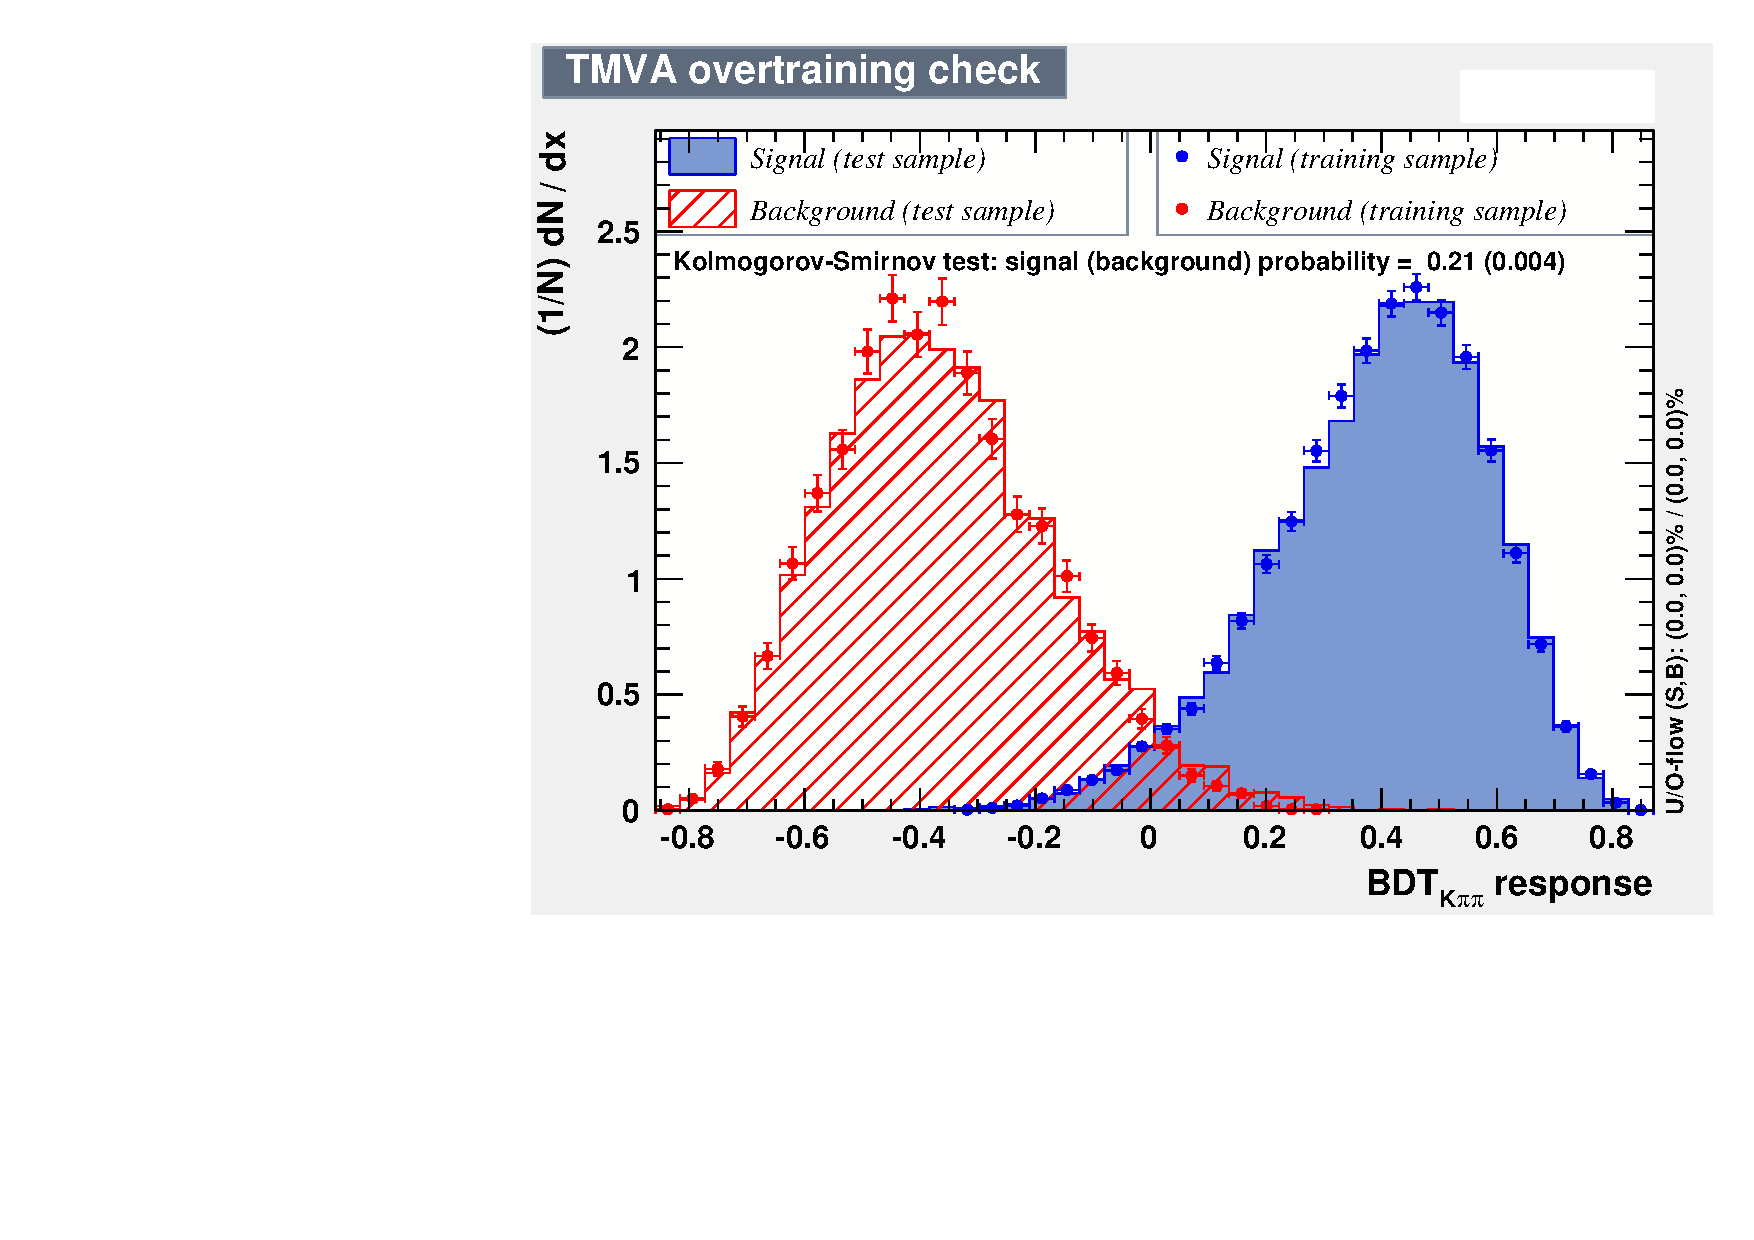
\includegraphics[width=0.48\textwidth]{07-B02DD/figs/Overtraining_Check_Kpipi.pdf}
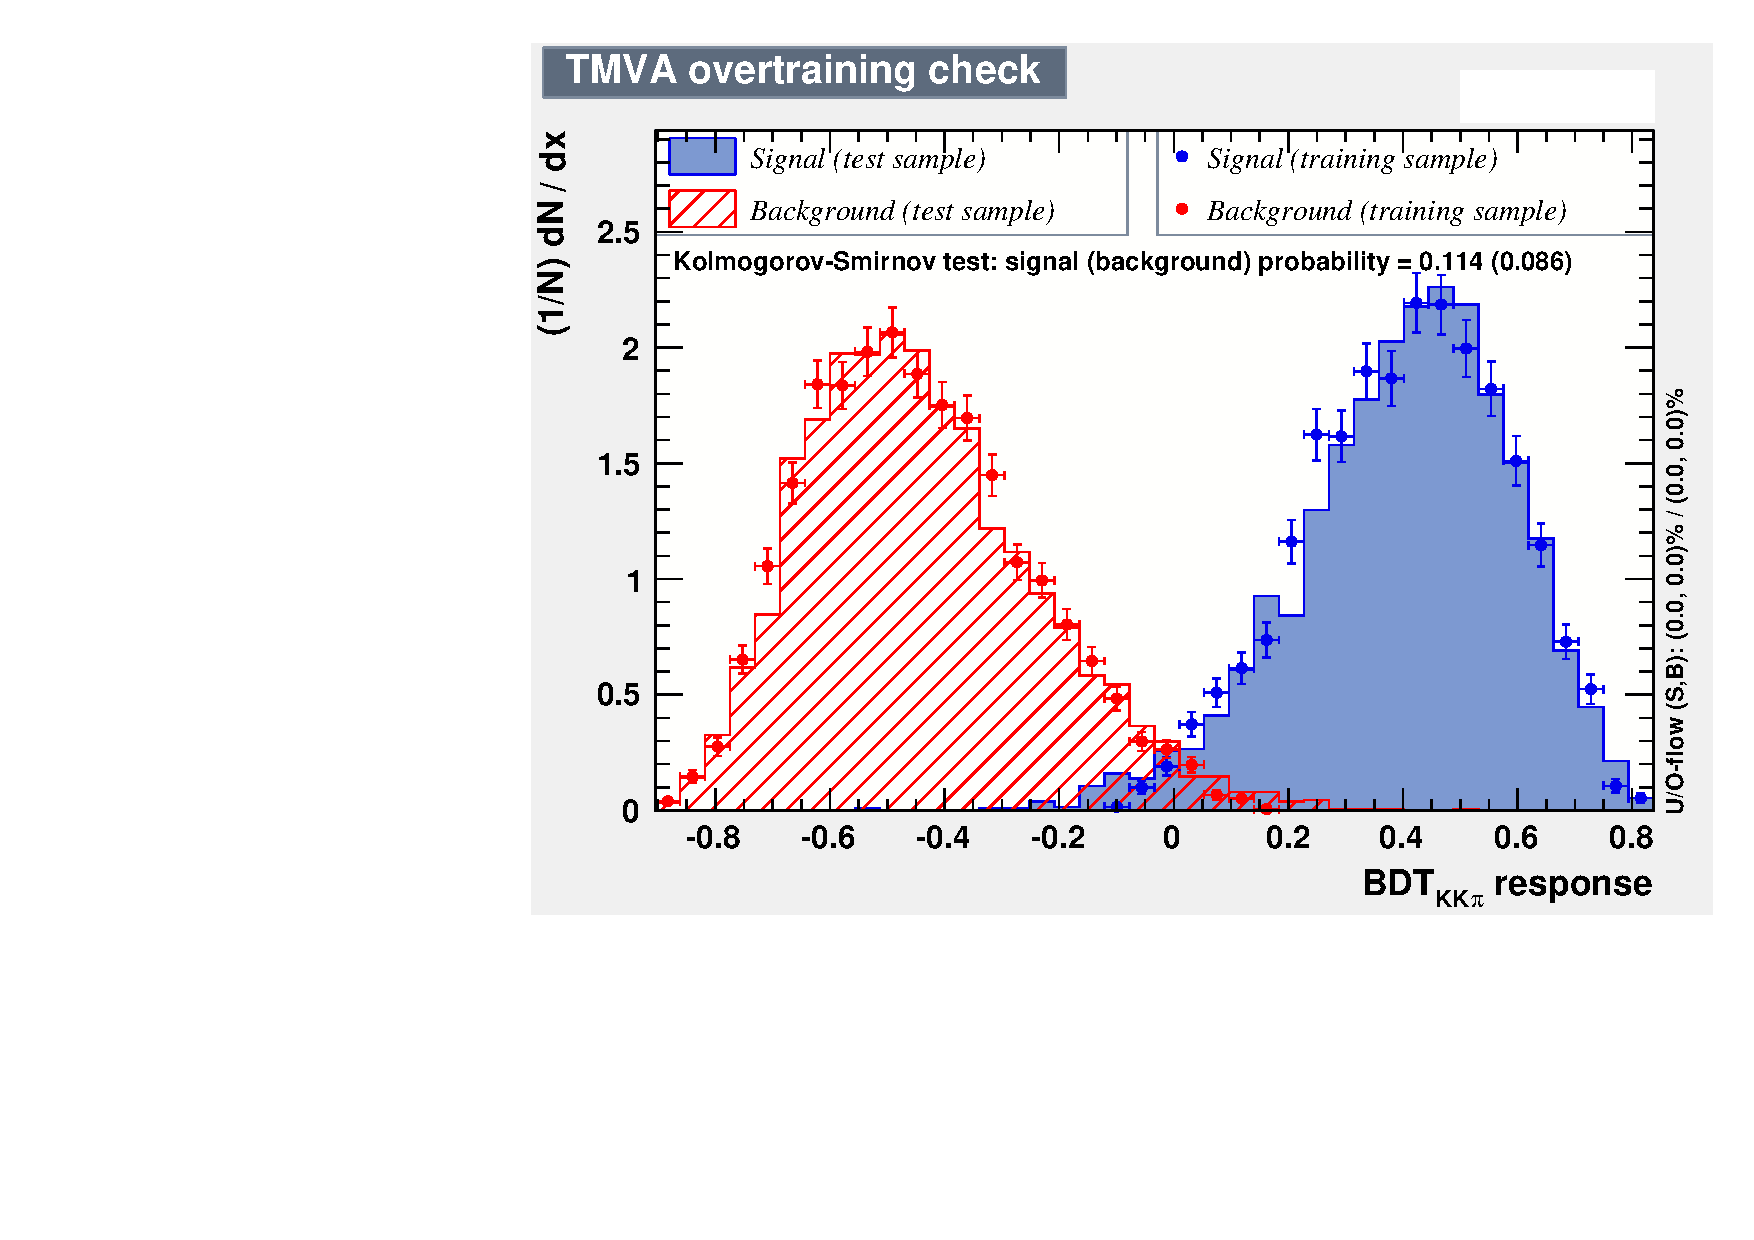
\includegraphics[width=0.48\textwidth]{07-B02DD/figs/Overtraining_Check_KKpi.pdf}
\caption{Comparison of the BDT response on training and test sample for the
\KpipiKpipi final state (left) and the \KKpiKpipi final state (right).}
\label{fig:b02dd:selection:mva:overtraining}
\end{figure}
%
Using simulations in the selection contains the possibility that certain
distributions are not modelled properly and differences between the simulation
and real data are exploited instead of differences between signal and
background. Indeed, the classifier output distributions of the signal MC and
background-subtracted data show a quite large disagreement for both final
states as can be seen in \cref{fig:b02dd:selection:mva:bdtcomparison}. The
performance is clearly overestimated in the training.
%
\begin{figure}[htbp]
    \centering
    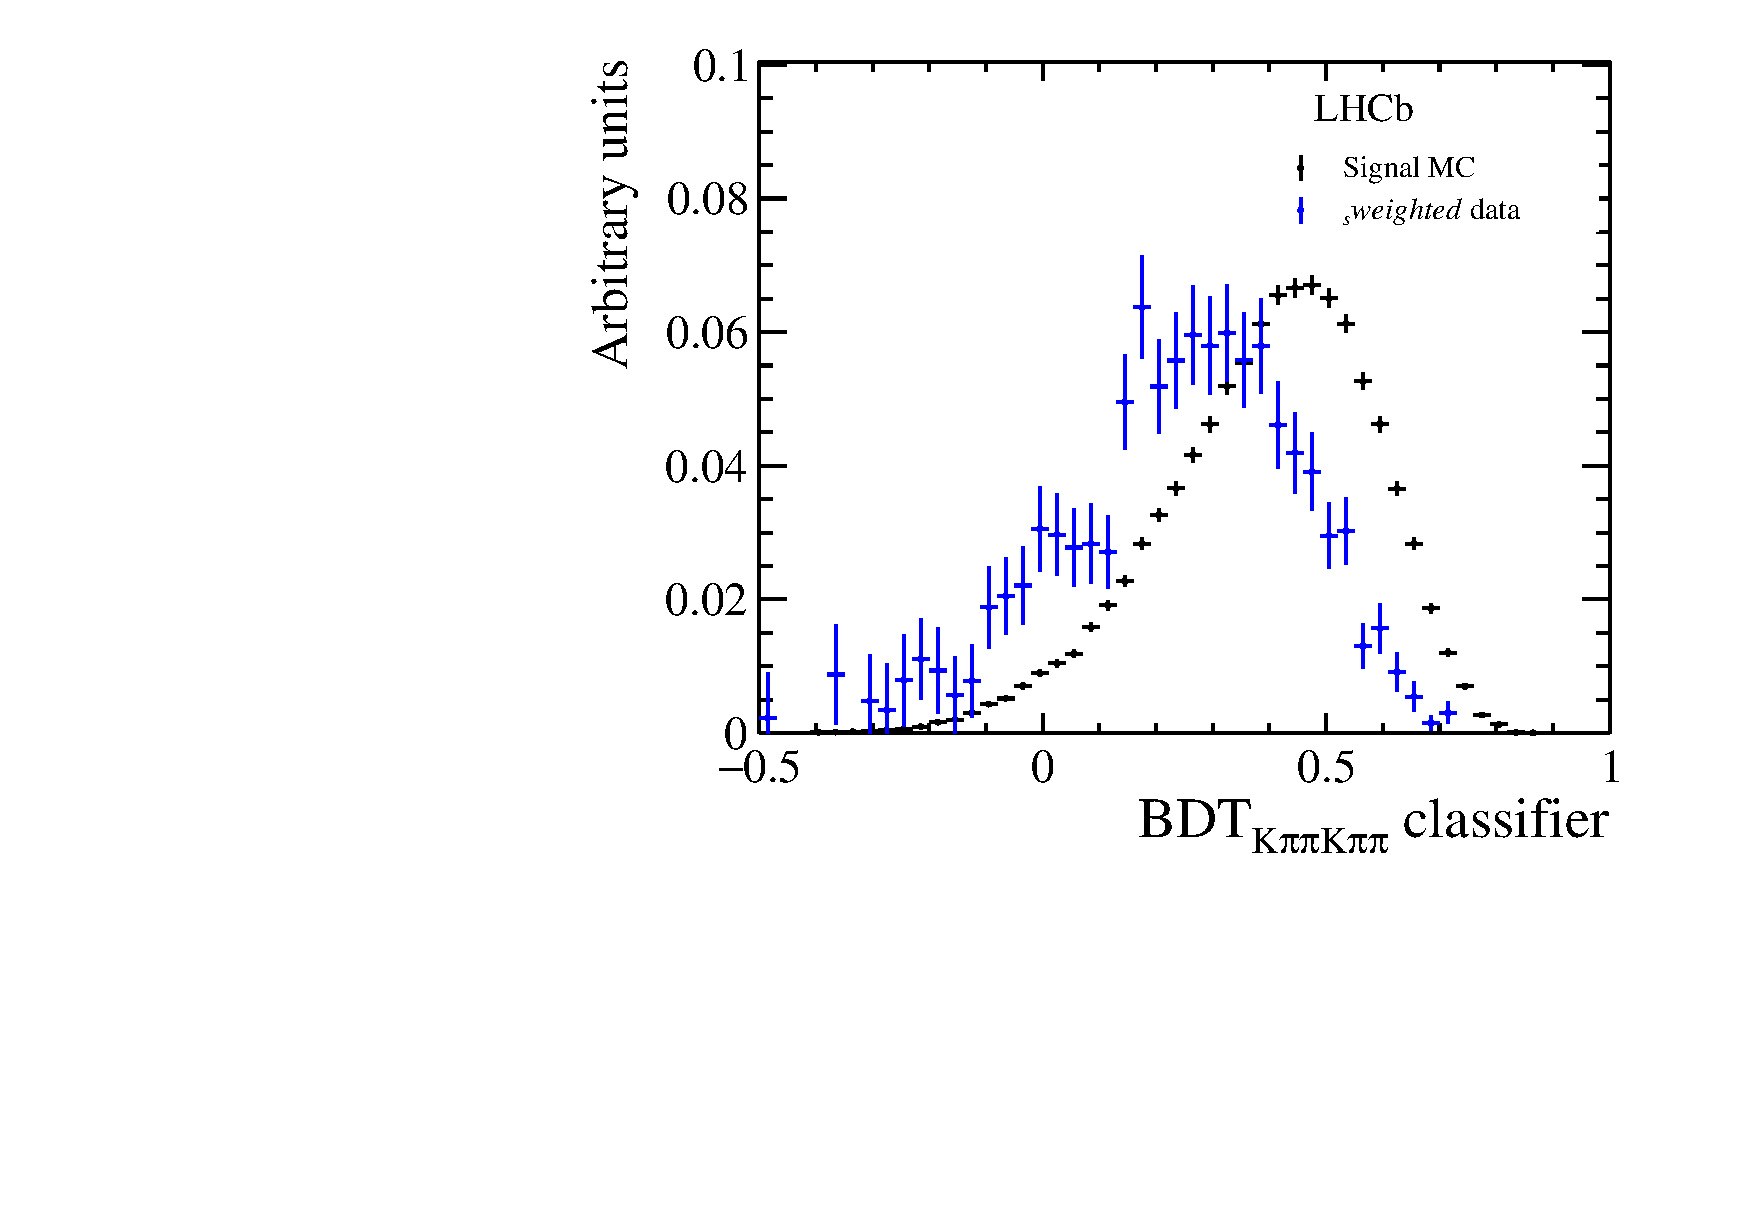
\includegraphics[width=0.49\textwidth]{07-B02DD/figs/BDTComparison_Kpipi.pdf}
    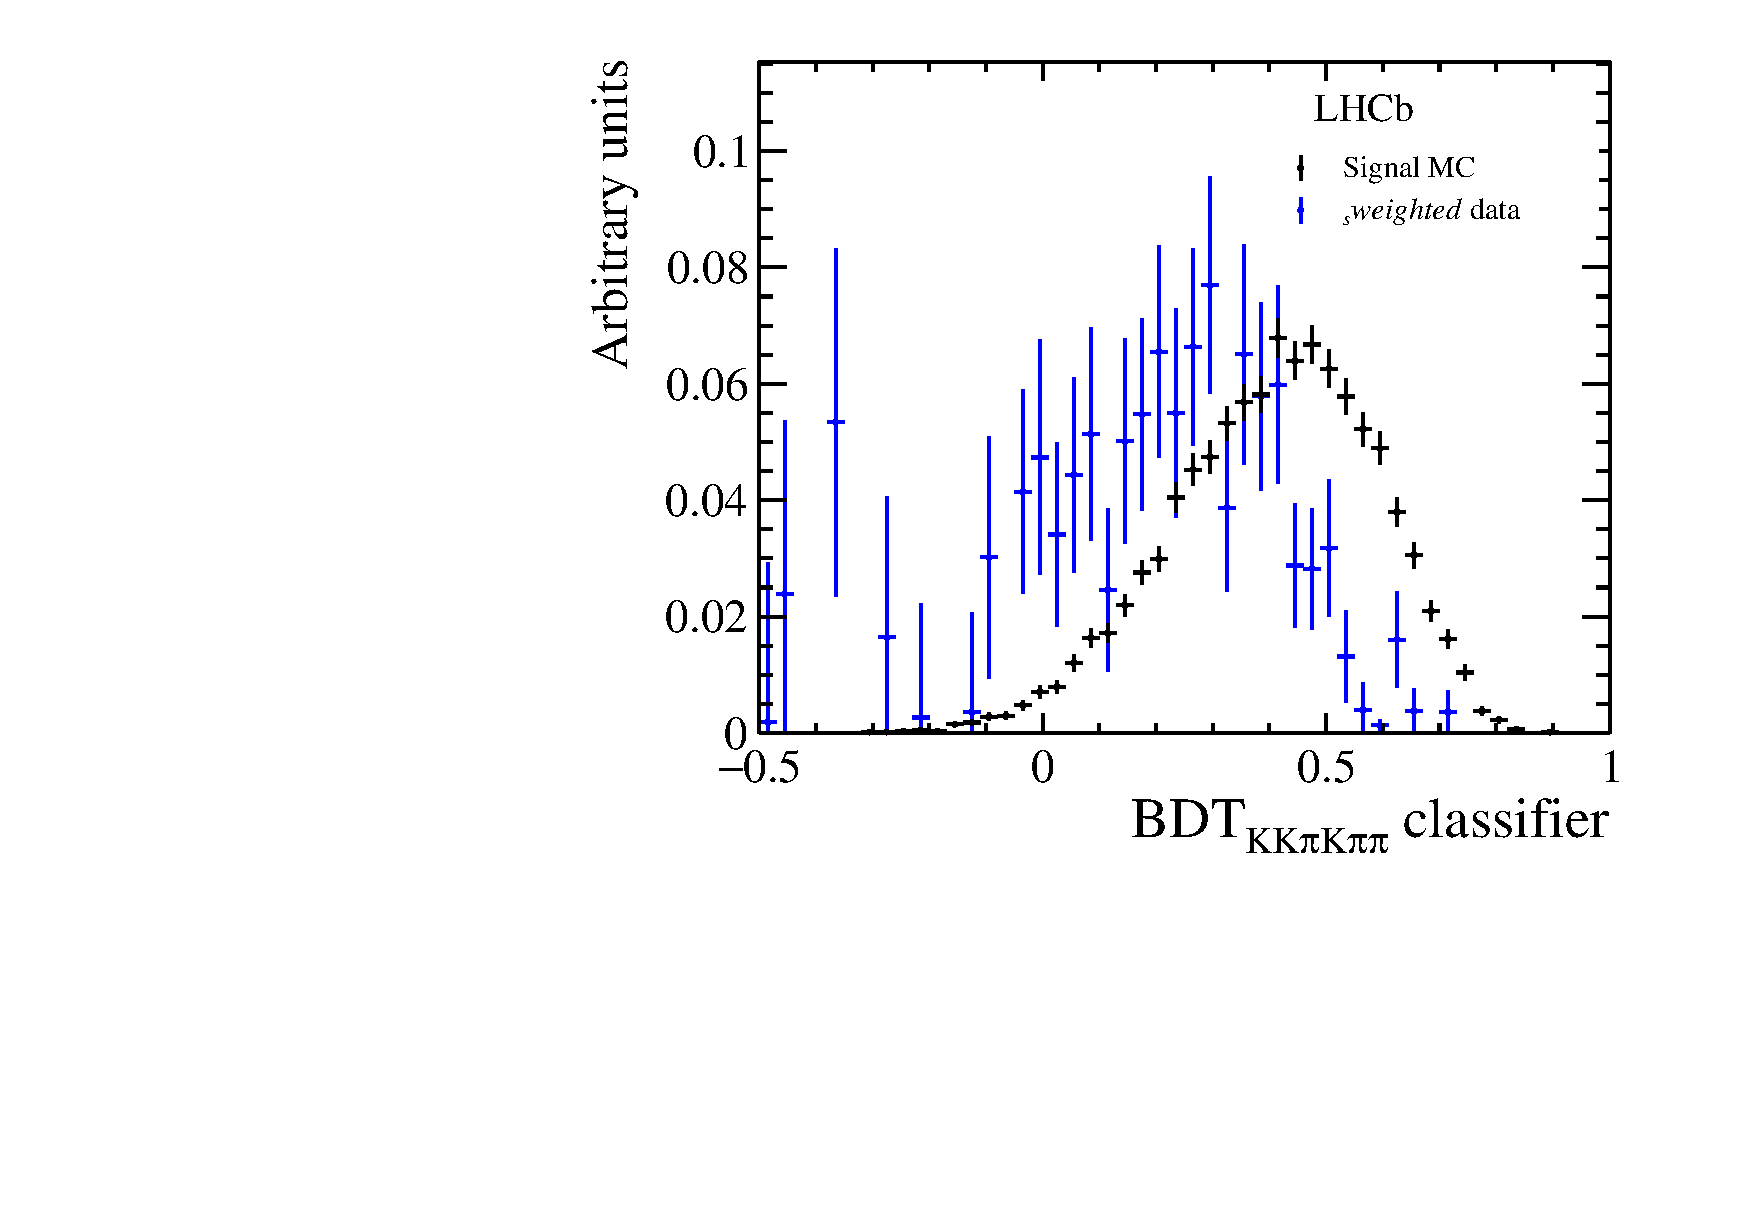
\includegraphics[width=0.49\textwidth]{07-B02DD/figs/BDTComparison_KKpi.pdf}
    \caption{Distribution of the BDT output for background-subtracted data (blue) and
    signal MC (black) for the \KpipiKpipi final state (left) and the
    \KKpiKpipi final state (right).}
    \label{fig:b02dd:selection:mva:bdtcomparison}
\end{figure}
%
This would be a problem if the selection efficiencies had to be calculated
using the MC sample. But for a measurement of \CP violation it is mainly
important that the amount of background can somehow be reduced while most of
the signal is kept. This can be achieved with the current setting.

% ==============================================================================
\subsubsection*{BDT cut optimisation}
\label{sec:b02dd:selection:mva:optimisation}

As explained in \cref{sec:dataanalysis:selection:fom} the best figure of merit
for a measurement of \CP violation is the sensitivity on the \CP observables
themselves. So the requirement on the BDT classifier output is scanned
performing a fit to the invariant $\Dp\Dm$ mass spectrum followed by a decay
time fit of the background-subtracted sample for each scan point. Initially,
only the subsample with two kaons in the \Bd final state is analysed. In
\cref{fig:b02dd:selection:mva:sensitivities} the statistical
uncertainties of \SDD and \CDD are plotted as a function of the requirement on
the BDT classifier output.
%
\begin{figure}[!htb]
\centering
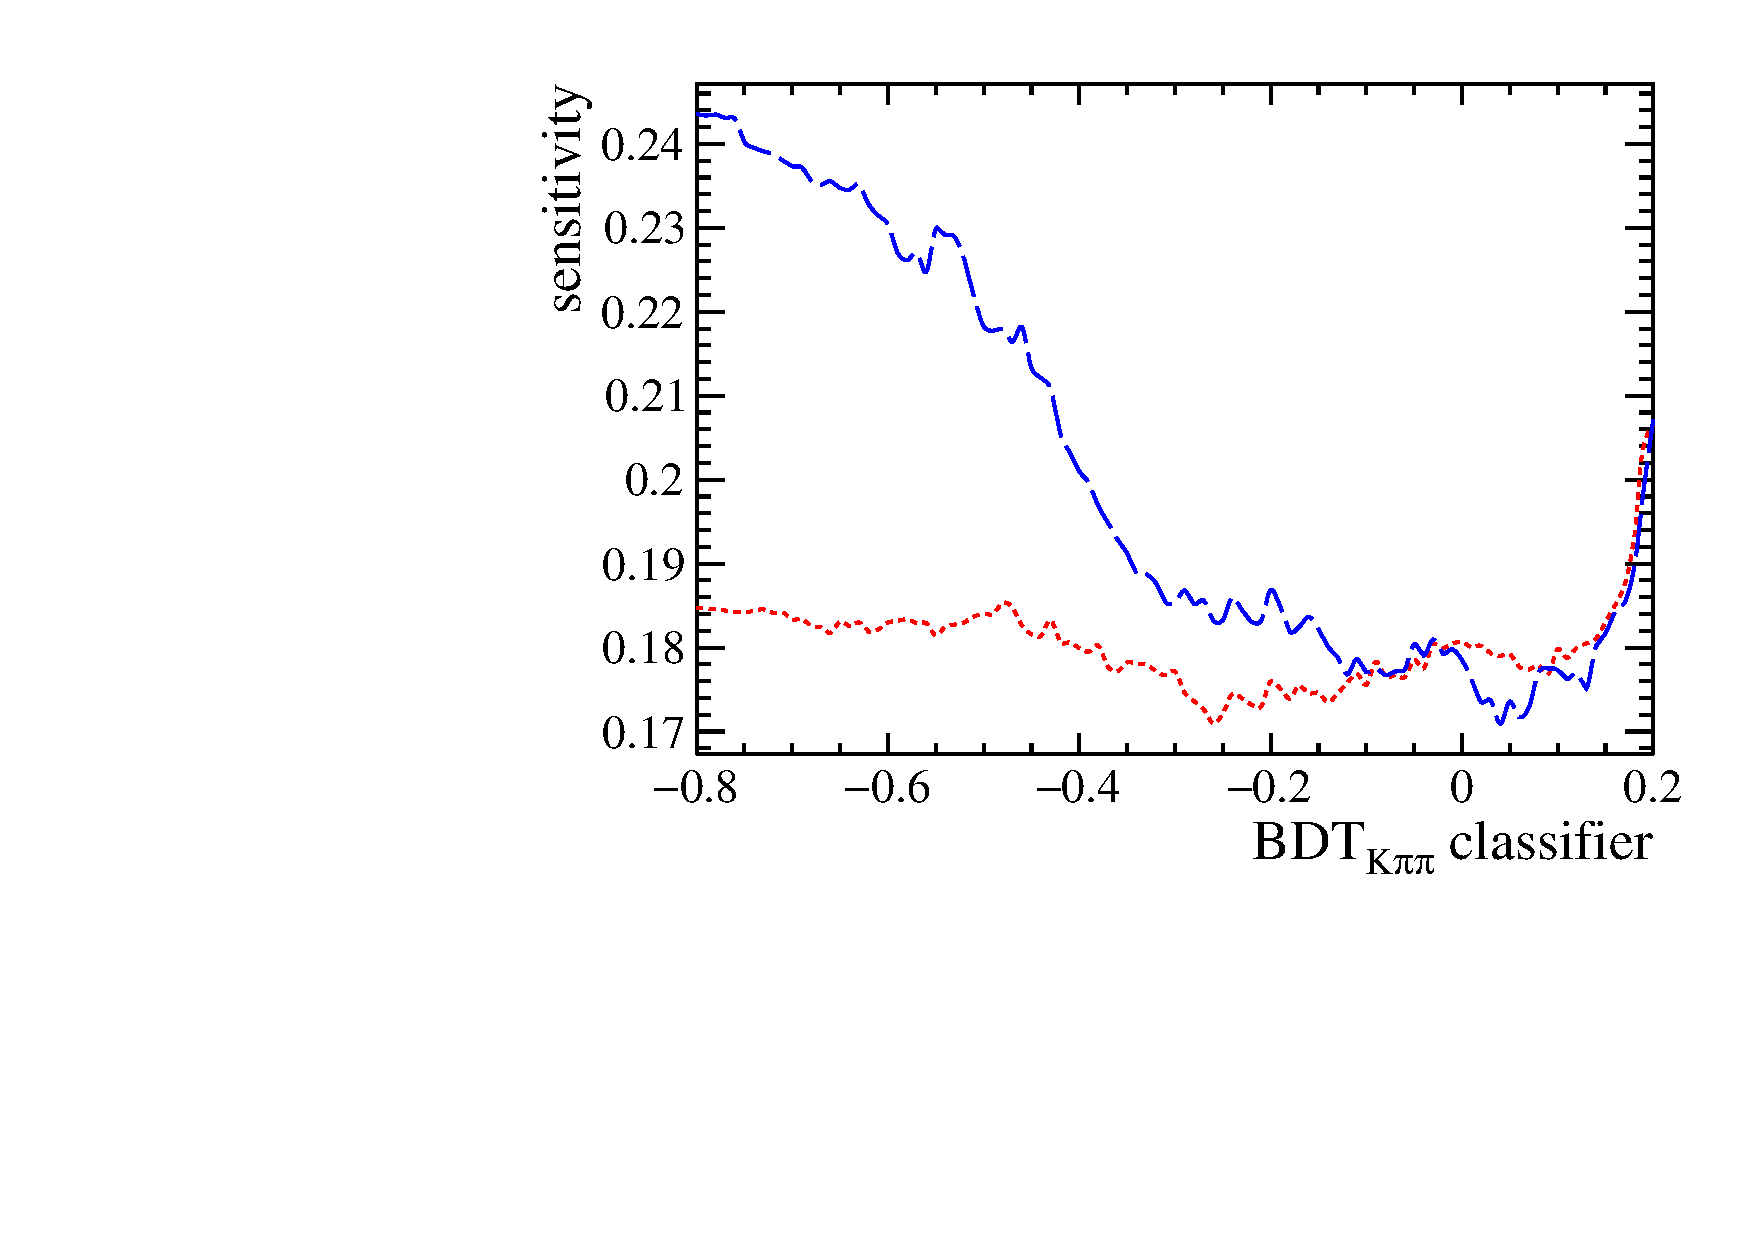
\includegraphics[width=0.48\textwidth]{07-B02DD/figs/Sensitivities_Kpipi.pdf}
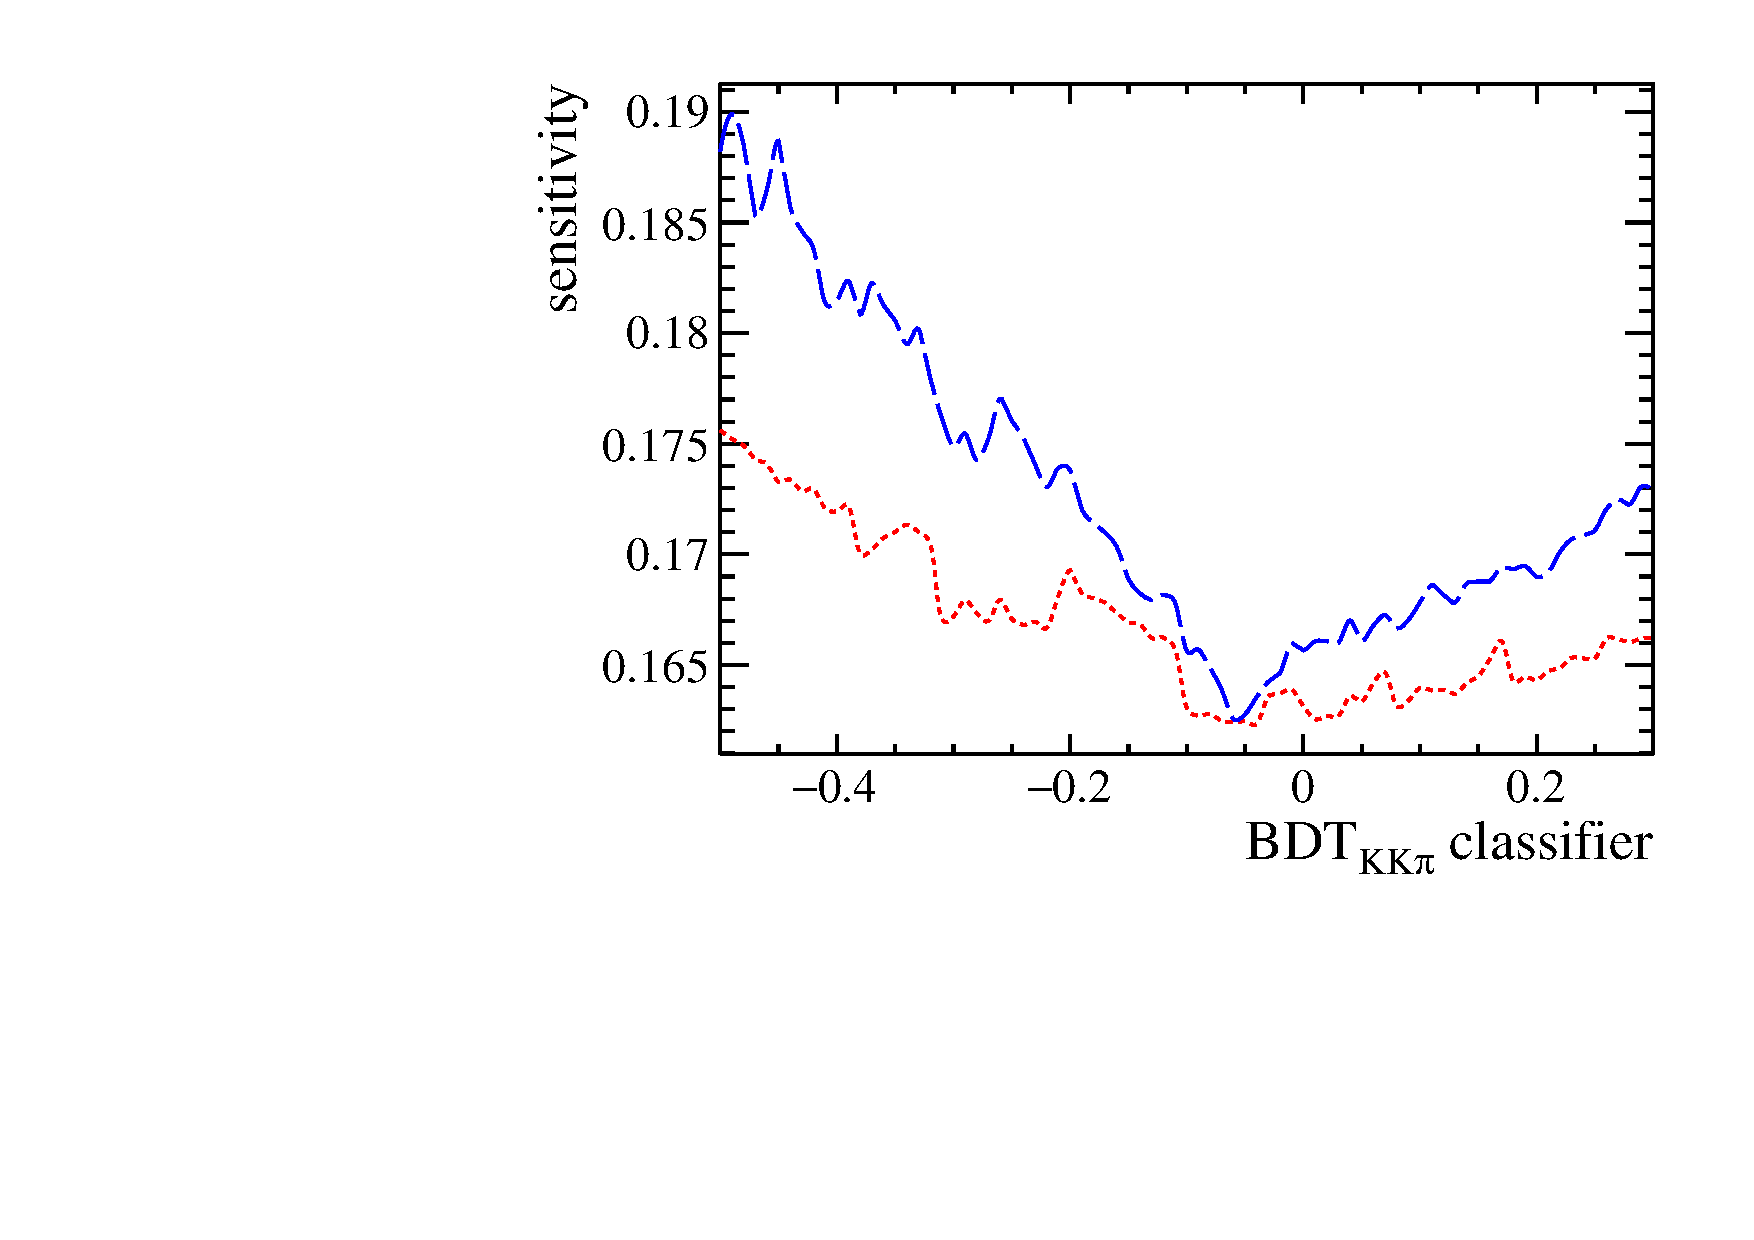
\includegraphics[width=0.48\textwidth]{07-B02DD/figs/Sensitivities_KKpi.pdf}
\caption{Sensitivity of \SDD (red short-dashed) and \CDD (blue long-dashed) as
a function of the BDT classifier output for the \KpipiKpipi final state (left)
and the \KKpiKpipi final state (right).}
\label{fig:b02dd:selection:mva:sensitivities}
\end{figure}
%
The uncertainty on \CDD improves with tighter requirements on the BDT
classifier until it reaches an optimum shortly after zero. This can be
explained with the fact that the sensitivity on \CDD mainly comes from
candidates at low decay times because the cosine function is maximal there.
The suppression of the rather short-lived combinatorial background compensates
the loss in signal efficiency for a quite long range. In contrast, the
uncertainty on \SDD is mainly driven by the amount of signal candidates. So it
is more or less flat for loose requirements on the BDT classifier where only
few signal candidates are lost and this is compensated by the higher purity
and reaches its optimum around \num{-0.25} before it starts to get worse. Now
that both observables are of interest and the optima are not at the same cut
value it is decided to require the BDT classifier to be greater than
\num{-0.10}. This is a good compromise between both observables as the
uncertainties of \SDD and \CDD are almost the same and close to their optima.
The requirement has a signal efficiency of \SI{96.5\pm0.5}{\percent} and
rejects \SI{84.18\pm0.34}{\percent} of the combinatorial background.

In a second step the requirement on the BDT classifier for the \KKpiKpipi
final state is optimised. The \KKpiKpipi subsample is quite small, which makes
individual fits on this subsample rather unstable. This can be solved by
performing a simultaneous fit to the whole dataset with the previously
determined BDT cut applied to the \KpipiKpipi subsample. Scanning the BDT
classifier output for the \KKpiKpipi final state results in the sensitivities
on \SDD and \CDD plotted in \cref{fig:b02dd:selection:mva:sensitivities}. Both
uncertainties show a minimum at around \num{-0.05}, which is chosen as cut
value. This cut removes \SI{90.75\pm0.33}{\percent} of the combinatorial
background at a signal efficiency of \SI{87.2\pm1.9}{\percent}.

\subsection{Final selection}
\label{sec:b02dd:selection:final_selection}

Finally, the fit range of the invariant $m_{\Dp\Dm}$ mass is reduced to
\SIrange{5150}{5500}{\MeVcc}, which eliminates some backgrounds, like
misreconstructed \mbox{\BdToDstD}, at low masses, prevents overtraining
effects on the high-mass sideband used in the training of the BDT, and leaves
enough candidates in the upper mass sideband to determine the shape of the
combinatorial background. Additionally, the decay time is restricted to be in
the range \SIrange{0.25}{10.25}{\ps} to avoid edge effects. In
\SI{0.8}{\percent} of the selected events more than one candidate remains,
which is very unlikely given the low branching branching fraction. So choosing
randomly only one of the multiple candidates is kept.


%!TEX root = ../main.tex

\section{Mass fit (5 pages)}
\label{sec:b02dd:massfit}

%!TEX root = ../main.tex

\section{Decay time fit}
\label{sec:b02dd:decaytimefit}

The conditional PDF describing the reconstructed decay time $t'$ and tag
decisions $\vect{d'} = (\dos, \dss)$, given a per-event decay time resolution
$\sigma_{t'}$ and per-event mistag probability estimates $\vect{\eta} = (\etaos,
\etass)$, is
%
\begin{equation}\label{eq:fullpdf}
  P\left(t',\vect{d'}\given \sigma_{t'},\vect{\eta}\right)
  \propto \epsilon(t') \left(\mathcal{P}(t,\vect{d'}\given \vect{\eta})
    \otimes \mathcal{R}(t'-t\given \sigma_{t'})\right)\,,
\end{equation}
%
where
\begin{equation}
  \mathcal{P}(t,\vect{d'}\given \vect{\eta}) \\
  \propto \sum_{d} \mathcal{P}(\vect{d'} \given d,\vect{\eta})
      [1 - d\, A_\text{P}] \,
      e^{-t/\tau}\left\{1 - d\, S \sin(\dm t) + d\, C \cos(\dm t)\right\}\,,
\end{equation}
and where $t$ is the true decay time, $d$ is the true production flavour,
$A_\text{P}$ is the production asymmetry, and $\mathcal{P}(\vect{d'} \given
d,\vect{\eta})$ is a two-dimensional binomial PDF describing the distribution
of tagging decisions given $\vect{\eta}$ and $d$. Normalisation factors are omitted for brevity.

%============================================================================%
%!TEX root = ../main.tex
\section{Decay time resolution}
\label{sec:dataanalysis::resolution}

Uncertainties in the determination of the position of vertices and in the
measurement of momenta (although thanks to the VELO (see
\cref{sec:detector:lhcb}) pretty accurate  at $\lhcb$) lead to a finite decay
time resolution $\sigma$, which dilutes the observed $\CP$ asymmetry by a
factor
\begin{align}
  \mathcal{D} = e^{\frac{-\dmd^2\,\sigma^2}{2}} \, .
\end{align}
This formula is the special case for a Gaussian resolution model with width
$\sigma$. The general formula is derived in
Ref.~\cite{ResolutionDilutionFactor}. For $\Bd$ mesons the dilution induced by
the decay time resolution has only minor influence on the measurement of $\CP$
observables because the oscillation frequency of $\Bd$ mesons $\dmd =
\SI{0.5064\pm0.0019}{\hbar\invps}$~\cite{HFAG} is quite low. Even for a decay time
resolution of \SI{100}{\fs}, which would be almost two times larger than what
is usually found in analyses performed by \lhcb, the dilution factor is
greater than \SI{99}{\percent}.

\FloatBarrier
%============================================================================%
%!TEX root = ../main.tex
\subsection{Decay time acceptance}
\label{sec:b02dd:decaytimefit:acceptance}

The trigger requirements as well as some input variables to the BDT result in
a decay-time-dependent efficiency. Additionally, the \velo reconstruction
(\ie the FastVelo algorithm~\cite{Callot:2011bza}) causes a drop in decay time
acceptance for events with large decay times. In order to correctly describe
these effects the $\Bd$ lifetime is constrained to its PDG value of $\tau =
\SI{1.519\pm0.005}{\ps}$~\cite{PDG2014} in the nominal fit and any deviation
of the decay time distribution (summed over the tags) from a pure exponential
shape is supposed to be described by cubic splines (see
\cref{sec:dataanalysis:splines}). Knots are positioned on the rising edge,
approximately at the turning point, and at the boundaries of the decay time
range, so at $\{\SIlist[list-final-separator={,
}]{0.25;0.8;2.0;10.25}{\ps}\}$. The normalisation of the splines is arbitrary
and it has been decided to fix the second to last spline coefficient to
$\num{1.0}$.

On signal MC the truth information is available so the shape of the decay time
acceptance can be separated from the exponential decay. This shape is compared
with the spline method described above. As the BDTs are trained and applied
separately for the two final states and might have different effects on the
shape of the decay time acceptance these two categories are studied
individually.

\begin{figure}[htb]
\centering
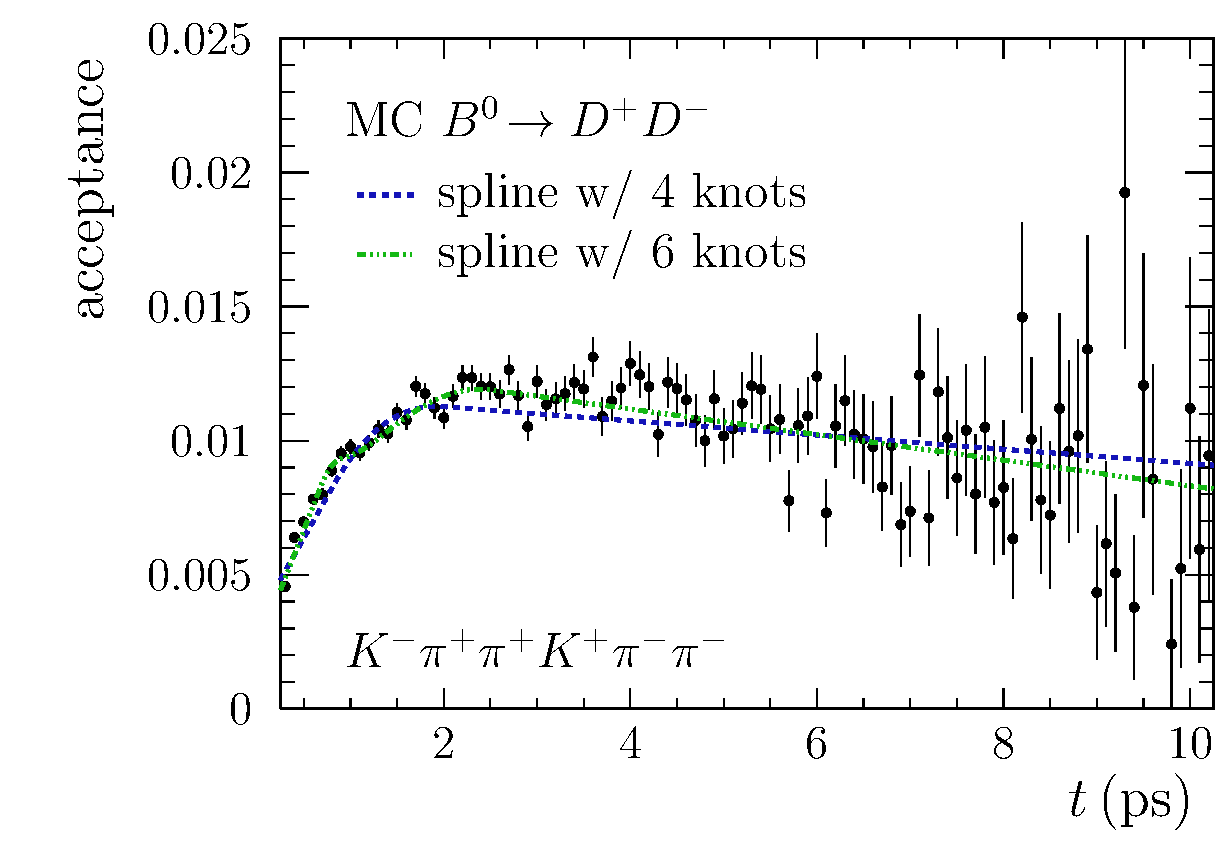
\includegraphics[width=0.48\textwidth]{07-B02DD/tikz/pdf/Acceptancespline_nolog_MC_Kpipi.pdf}
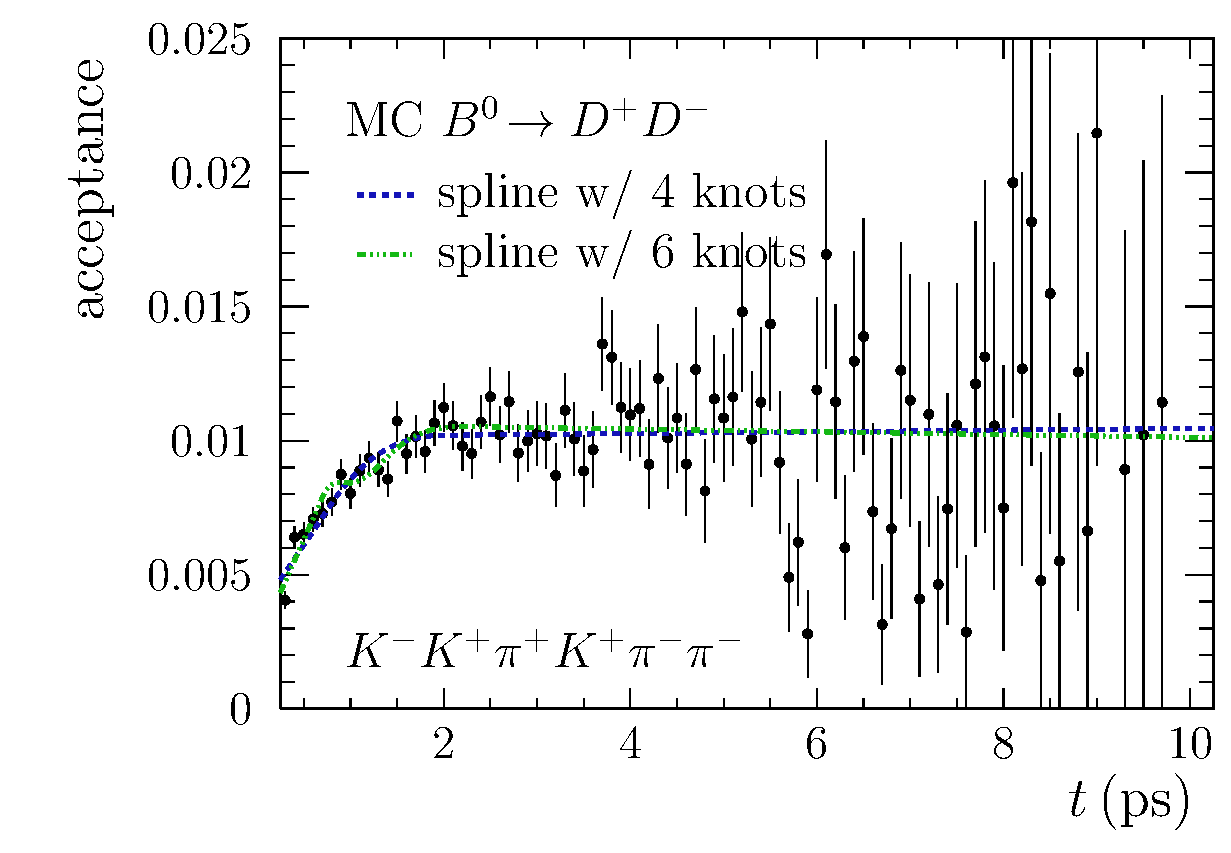
\includegraphics[width=0.48\textwidth]{07-B02DD/tikz/pdf/Acceptancespline_nolog_MC_KKpi.pdf}
\caption{Decay time acceptance of truth-matched signal MC for the $\KpipiKpipi$
final state (left) and the $\KKpiKpipi$ final state (right). The black data
points show the true decay time acceptance determined by dividing the
reconstructed by the true decay time distribution. The blue line is the spline
acceptance function and the red stripes indicate the $1\,\sigma$ error band
taking into account the statistical uncertainties.}
\label{fig:b02dd:decaytimefit:acceptance_MC}
\end{figure}

Looking at the plots in \cref{fig:b02dd:decaytimefit:acceptance_MC} it is
apparent that compared to $\BdToJPsiKS$ there is a quite large efficiency loss
at high decay times. This might be related to the fact that both $\Bd$
daughter particles ($\Dp$ and $\Dm$) are relatively long-lived. The true MC
decay time acceptance is overlaid with the shape of two spline functions.
Besides the spline function with the nominal number of four knots an
additional spline function with two more knots and slightly changed positions
$(\SIlist[list-final-separator={, }]{0.25;0.7;1.0;1.5;2.5;10.25}{\ps})$ is
plotted, which gives a better description. But it has to be considered that
the statistics of the MC sample is \num{25} times larger than the real data.
Therefore, the spline function with four knots is chosen, otherwise rather
statistical fluctuations than acceptance effects would be described. The low
statistics of the $\KKpiKpipi$ final state on real data does also not allow to
use separate spline coefficients for the two final states although with the
increased MC statistics some differences become visible.


\FloatBarrier
%============================================================================%
\subsection{External inputs}
\label{sec:b02dd:decaytimefit:constraints}

\lhcb has performed a measurement of the production asymmetry as a function
of transverse momentum and pseudorapidity using \SI{7}{\TeV}
data~\cite{LHCb-PAPER-2014-042}. Taking those distributions from \BdToDD
individual weighted averages for the 2011 and 2012 subsamples are calculated
yielding
%
\begin{equation}
  \begin{split}
    \prodasym{11} &= -0.0047 \pm 0.0106 \,\text{(stat)} \pm 0.0014 \, \text{(syst)} \,, \\
    \prodasym{12} &= -0.0071 \pm 0.0107 \,\text{(stat)} \pm 0.0014 \, \text{(syst)} \,.
  \end{split}
\end{equation}
%
As the measurement of the production asymmetry has been performed on 2011 data
only, the numbers for $\prodasym{11}$ and $\prodasym{12}$ are highly
correlated. So, the latter is modelled as $\prodasym{12} = \prodasym{11} +
\Delta\prodasym{}$ with $\Delta\prodasym{} = -0.0024 \pm 0.0018
\,\text{(syst)}$. The systematic uncertainty accounts for the difference of
the production asymmetries observed for the two data-taking conditions in the
measurement of the semileptonic $\CP$ asymmetry~\cite{LHCb-PAPER-2014-053} and
is used as the width of a Gaussian constraint. The $\Bz$ oscillation frequency and
the $\Bz$ lifetime are constrained to $\dm =
\SI{0.510\pm0.003}{\planckbar\invps}$~\cite{PDG2014} and $\tau =
\SI{1.519\pm0.005}{\ps}$~\cite{PDG2014}, respectively. The
flavour-tagging calibration parameters
(\cref{tab:dataanalysis:taggingcalibration:dsdcalibration}) are constrained
within their combined statistical and systematic uncertainties, determined in
the calibration using \BdToDsD decays. The decay time resolution parameters
(\cref{tab:b02dd:decaytimefit:resolution}) and the $\Bz$ lifetime difference
$\DG = \SI{0}{\invps}$ are fixed in the likelihood fit.

%============================================================================%
\subsection{Results}

The fit results of the $\CP$ observables from the decay time fit are
\begin{align}
\begin{split}
  \SDD                &= -0.54\,\pm\,^{0.17}_{0.16} \, , \\
  \CDD                &= \phantom{-}0.26\,\pm\,0.17 \, , \\
  \rho(\SDD,\CDD)     &= \phantom{-}0.48 \, . \\
\end{split}
\label{eq:b02dd:decaytimefit:cpresults}
\end{align}

Only after rescaling the sWeights via
\begin{align}
  w_i = w_i \frac{\sum w_i}{\sum w_i^2}\,,
\end{align}
correct asymmetric uncertainty estimates are delivered by \minos, which is
\root's standard method to analyse the likelihood shape. To check if the
coverage is guaranteed the bootstrapping method is applied. The nominal fit
procedure, \ie performing the mass fit, calculating the sWeights and fitting
the weighted tagged decay time distribution, is executed and the fit results
are stored. The drawing and fitting is done \num{10000} times. It turns out
that half of the fits fail if the flavour-tagging calibration parameters are
constrained within their statistical uncertainties. When fixing them to their
central values the fit failure rate drops to a per-mille effect. From the
distribution of fit results the two-side \SI{68}{\percent} confidence
intervals are extracted. To account for the uncertainties on the
flavour-tagging calibration parameters \num{10000} pseudoexperiments are
performed, in which the nominal model is used to generate the signal decay
time distribution and the fit results of the nominal fit are chosen for the
\CP observables \SDD and \CDD. Before generating the flavour-tagging
calibration parameters are drawn from Gaussian distributions around their
central values using the combined statistical + systematic uncertainties. In
the subsequent fit the flavour-tagging calibration parameters are fixed to
their central values, like in the fits to the bootstrapped samples. The
resulting pull distributions are broader than standard normal distributions.
The deviation of the width from unity shows how much the statistical
uncertainties are underestimated in the likelihood fit due to not accounting
for the variation of the flavour-tagging calibration parameters. So, the
statistical uncertainties for \SDD and \CDD from the bootstrapping including
the impact of the uncertainty of the flavour-tagging calibration parameters
are given by scaling the bootstrapping uncertainties by the width of the pull
distributions:
\begin{align}
    \sigma_{\SDD}(\text{bootstrapping}) &= \,^{+0.17}_{-0.16} \,, \\
    \sigma_{\CDD}(\text{bootstrapping}) &= \,^{+0.18}_{-0.17} \,.
\end{align}
These uncertainties match the nominal ones from \minos quite well. A plot of
the decay time distribution and the projection of the acceptance model are
shown in \cref{fig:b02dd:decaytimefit}. Good agreement between the latter and
the shape on signal MC (cf. \cref{fig:b02dd:decaytimefit:acceptance_MC}) can
be observed but the low statistics leading to rather large uncertainties
indicated by the error band diminishes the significance of the comparison.

\begin{figure}[htb]
\hspace*{\fill}
\begin{minipage}{0.4\textwidth}
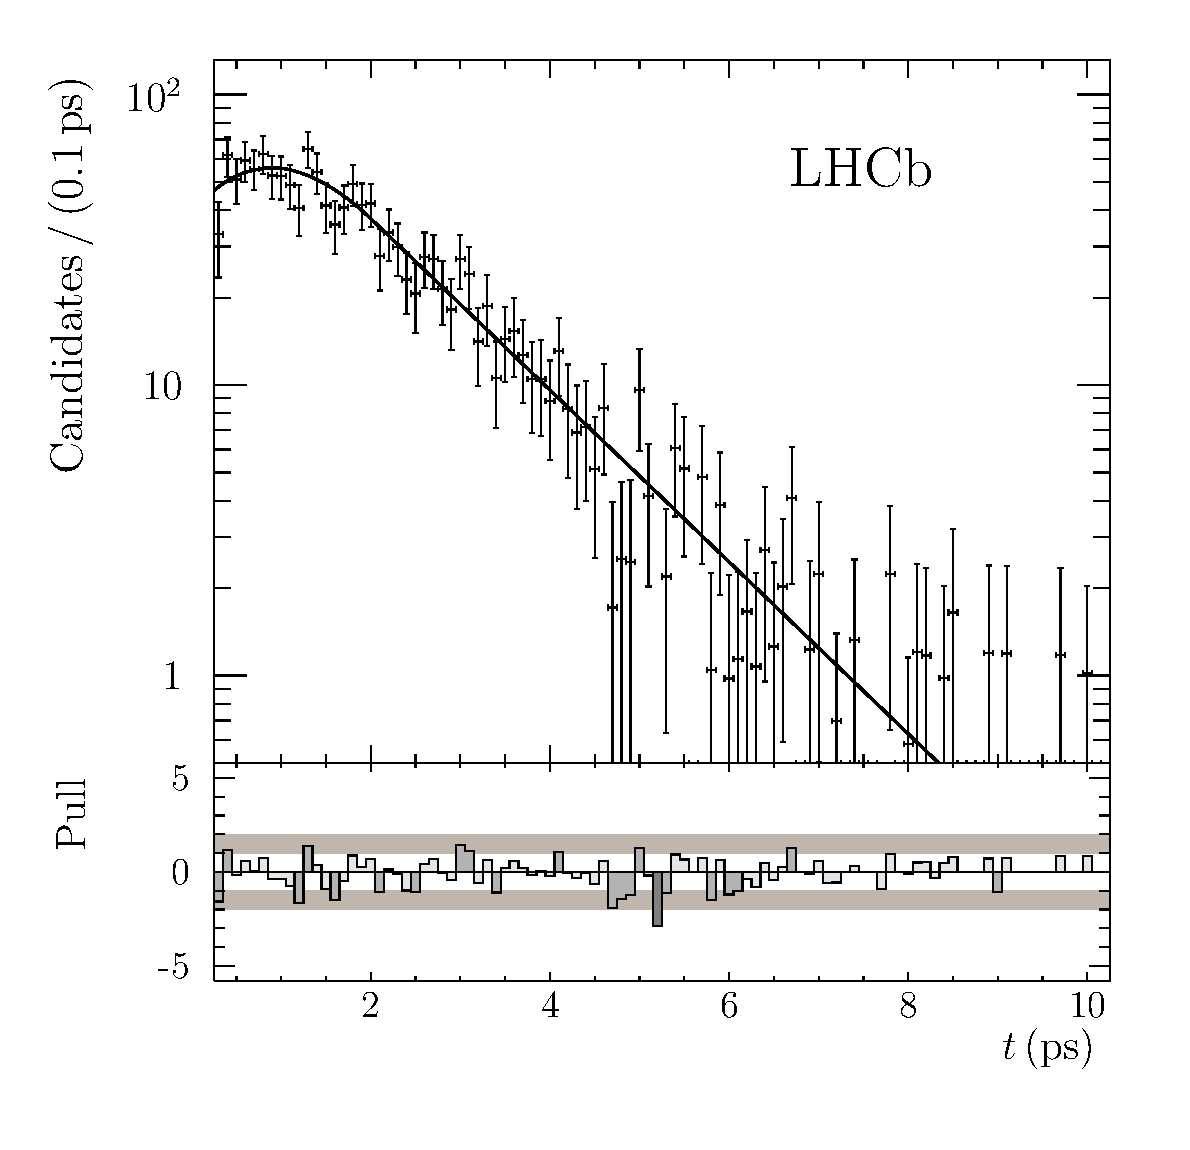
\includegraphics[width=\textwidth]{07-B02DD/tikz/pdf/obsTime_summed_pull_logy.pdf}
\end{minipage}
\hfill
\begin{minipage}{0.5\textwidth}
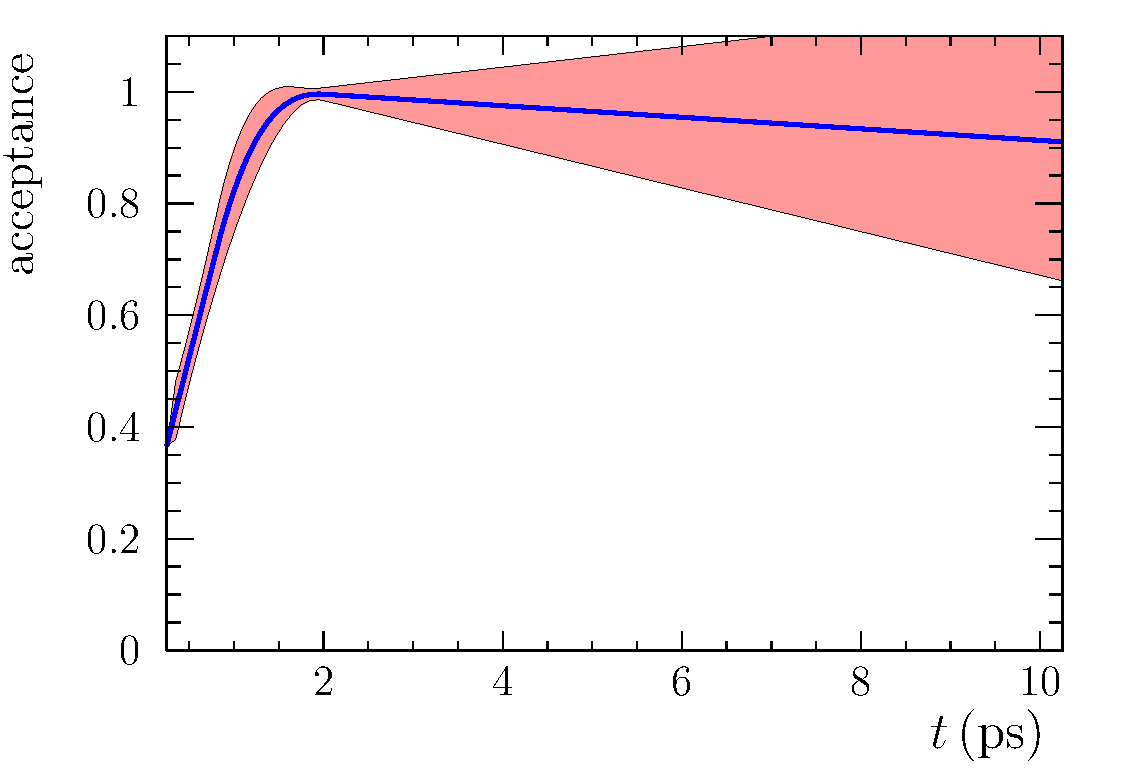
\includegraphics[width=\textwidth]{07-B02DD/tikz/pdf/Acceptancespline_nolog.pdf}
\end{minipage}
\hspace*{\fill}
\caption{Plot of the decay time distribution of the background-subtracted \BdToDD
data sample with the projection of the \PDF and the pull distribution on the
left. The y-axis is plotted in logarithmic scale. Plot of the nominal decay
time acceptance model on the right. The red area indicates the 1\,$\sigma$
error band taking into account the statistical uncertainties.}
\label{fig:b02dd:decaytimefit}
\end{figure}

Apart from a quite high positive correlation between the parameters of the
acceptance spline function and the already quoted correlation of about
\num{0.5} between $\SDD$ and $\CDD$, which is expected from first principles
(see Ref.~\cite{LHCb-ANA-2011-004}), no large correlation between fitted parameters
is present as can be seen from the correlation matrix visualised in
\cref{fig:b02dd:decaytimefit:FullFitCorrMatrixHotCold}. A possible correlation
between $\dm$ and $\CDD$ is significantly reduced by the constraint applied on $\dm$,
which is a lot tighter than the sensitivity accessible from the data sample.
When releasing this constraint the correlation coefficient becomes \num{-0.8}.
But the sensitivity on $\CDD$ would significantly decrease in this scenario, so
the constraint on $\dm$ is maintained in the nominal setup.

\begin{figure}[htb]
\centering
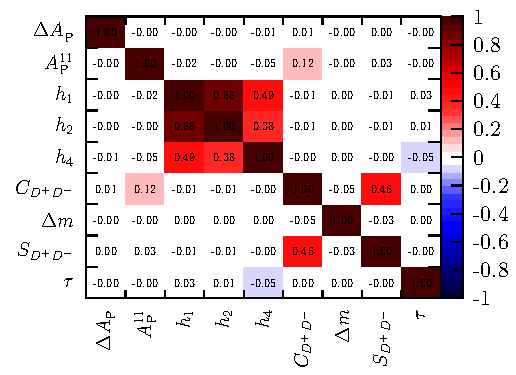
\includegraphics[width=0.5\textwidth]{07-B02DD/tikz/pdf/FitResultsCorrMatrix_RedBlueDiscrete_wText.pdf}
\caption{Visualised correlation matrix of the fit parameters in the decay time
fit to data. Positive correlations are represented by the red palette on the $z$ axis,
while negative correlations are represented by the blue palette of the $z$
axis.}
\label{fig:b02dd:decaytimefit:FullFitCorrMatrixHotCold}
\end{figure}

The 1D likelihood scans in \cref{fig:b02dd:decaytimefit:1DLLScan} show a nice
parabolic shape with a clear minimum.
\begin{figure}[htb]
\centering
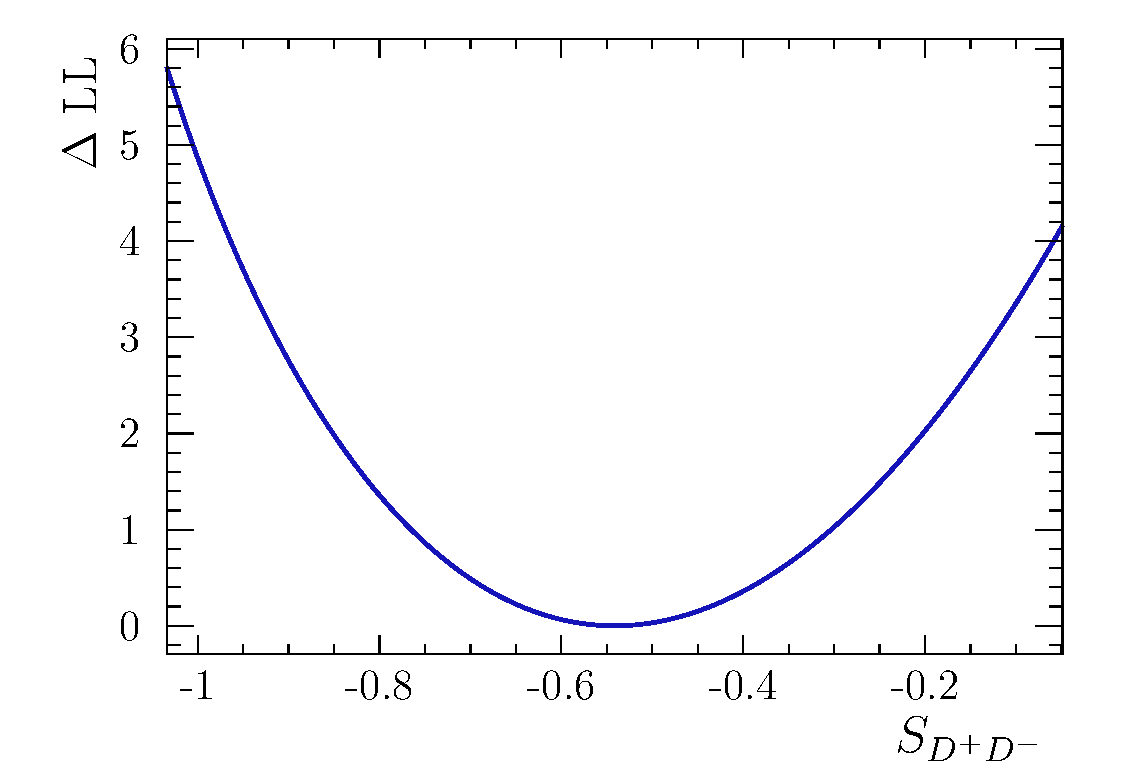
\includegraphics[width=0.48\textwidth]{07-B02DD/tikz/pdf/Likelihoodscan_sin2b.pdf}
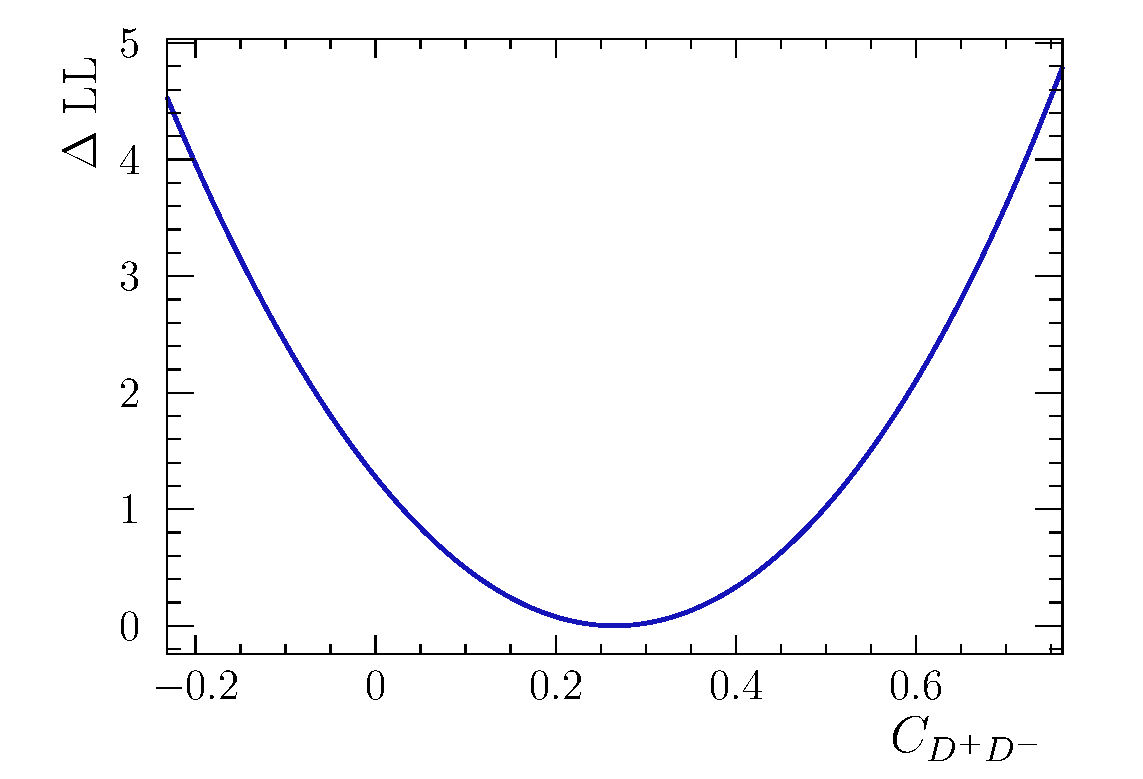
\includegraphics[width=0.48\textwidth]{07-B02DD/tikz/pdf/Likelihoodscan_C.pdf}
\caption{One-dimensional likelihood profile scans for $\SDD$ and $\CDD$.}
\label{fig:b02dd:decaytimefit:1DLLScan}
\end{figure}

In \cref{fig:b02dd:decaytimefit:asymmetry} the signal yield asymmetry is
plotted in eight bins of the decay time. A binned $\chisq$-fit to this signal
asymmetry is performed using
\begin{align}
{\mathcal A}^{\text{meas}}(t) = \frac{\Delta\omega + \prodasym{11}(1 - 2\omega) + (1 - 2\omega + \prodasym{11}\Delta\omega){\mathcal A}^{\text{theo}}(t)}{1 + \prodasym{11}(\SDD \sin(\dm\,t) - \CDD \cos(\dm\,t))}\,,
\label{eq:b02dd:decaytimefit:asymmetry_td}
\end{align}
which is a modified version of the theoretical signal asymmetry in
\cref{eq:cpviolation:simpleasymmetry} and accounts for the mistag probability
\mistag and the asymmetries induced by flavour tagging ($\Delta\omega$) and
production asymmetry ($\prodasym{11}$). The fit results
\begin{align*}
\begin{split}
  \SDD                &= -0.65\,\pm\,0.25 \,, \\
  \CDD                &= \phantom{-}0.24\,\pm\,0.26 \,,
\end{split}
\end{align*}
are compatible with those from the unbinned fit presented in
\cref{eq:b02dd:decaytimefit:cpresults} but not as sensitive.
\begin{figure}[htb]
\centering
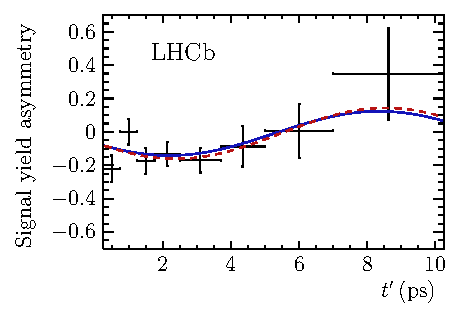
\includegraphics[width=0.48\textwidth]{07-B02DD/tikz/pdf/Asymmetry.pdf}
\caption{Decay-time-dependent signal yield asymmetry. The solid blue curve is the
projection of the signal PDF given in \cref{eq:fullpdf} and the dashed red curve is the
pure time-dependent fit function from
\cref{eq:b02dd:decaytimefit:asymmetry_td}}
\label{fig:b02dd:decaytimefit:asymmetry}
\end{figure}

\FloatBarrier


%!TEX root = ../main.tex

\section{Studies of systematic effects (5 pages)}
\label{sec:b02dd:systematics}

%============================================================================%
\subsection{Cross-checks}
\label{sec:systematics:xchecks}
To check for possible systematic effects, fits in different subsamples of the
nominal data set are performed. The cross-checks are performed for the two
tagging algorithms (OS vs. SS (not exclusive samples)), the two years of
data-taking (2011 vs. 2012) , combinations of those, the magnet polarities (Up
vs. Down), the two final states ($\KpipiKpipi$ vs. $\KKpiKpipi$) and for four
different slices of the BDT classifier for the $\KpipiKpipi$ final state.

\begin{figure}[thb]
\centering
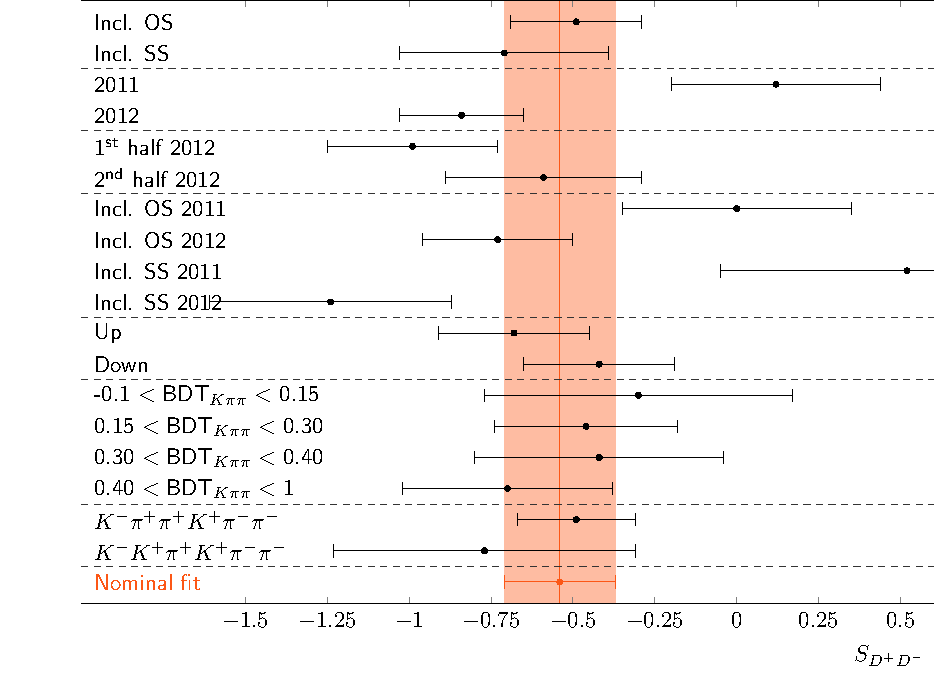
\includegraphics[width=0.9\textwidth]{07-B02DD/tikz/pdf/SComparison.pdf}
\caption{
Comparison of fit results of \SDD for fits on various subsamples.}
\label{fig:b02dd:systematics:xchecks:subsamples:s}
\end{figure}
\begin{figure}[thb]
\centering
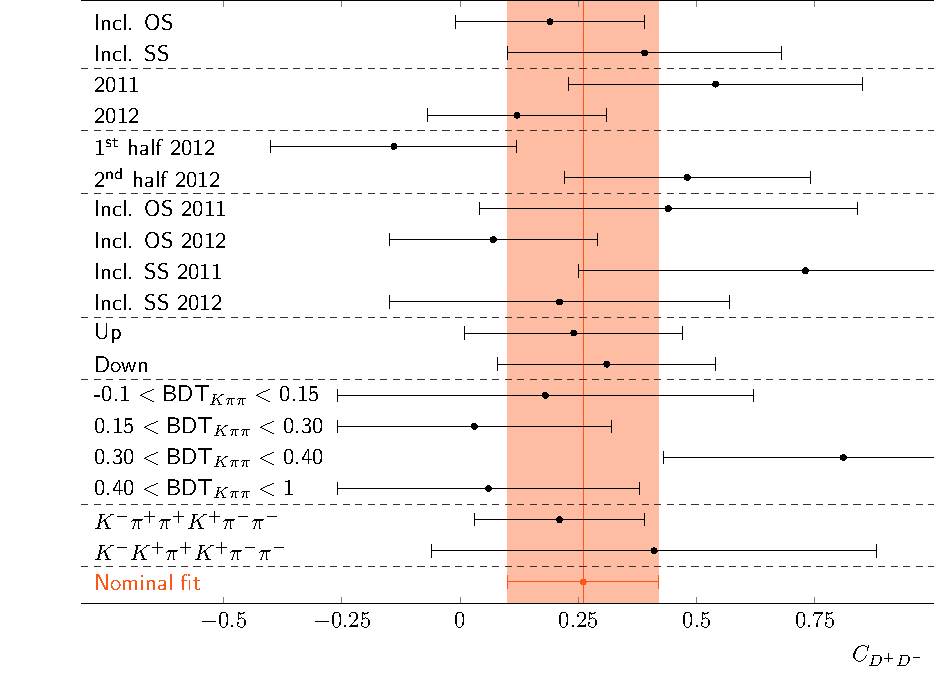
\includegraphics[width=0.9\textwidth]{07-B02DD/tikz/pdf/CComparison.pdf}
\caption{
Comparison of fit results of \CDD for fits on various subsamples.}
\label{fig:b02dd:systematics:xchecks:subsamples:c}
\end{figure}
The fit results in the various scenarios are illustrated in
\cref{fig:b02dd:systematics:xchecks:subsamples:s,fig:b02dd:systematics:xchecks:subsamples:c}.
While almost all splits show compatible results a rather large difference can
be observed between the 2011 and the 2012 subsample for $\SDD$. This is even
more pronounced when using only SS tagging. When determining the flavour
tagging calibration parameters separately for 2011 and 2012 data small
non-significant differences are observed but these can not explain the
different results of the $\CP$ observables. So the best explanation is that
the difference is due to a statistical fluctuation.

For the nominal fit the decay times and the decay time errors from the DTF are
used. The central values of the $\CP$ observables slightly change when using
the decay time (error) from the LVF, $\SDD = \num{-0.539}$ (LVF) vs.
\num{-0.541} (DTF) and $\CDD = \num{0.266}$ (LVF) vs. \num{0.263} (DTF). But
this difference is clearly below the statistical significance.

\FloatBarrier

%============================================================================%
\subsection{Decay Time Fit Bias}
\label{sec:b02dd:systematics:fitbias}

The likelihood fit itself might be biased. The nominal fit results for the
$\CP$ observables are used to generate \num{10000} pseudoexperiments. The pull
distributions in \cref{fig:b02dd:systematics:fitbias:pulls} show a very small
deviation of the mean value from zero.
%
\begin{figure}[htb]
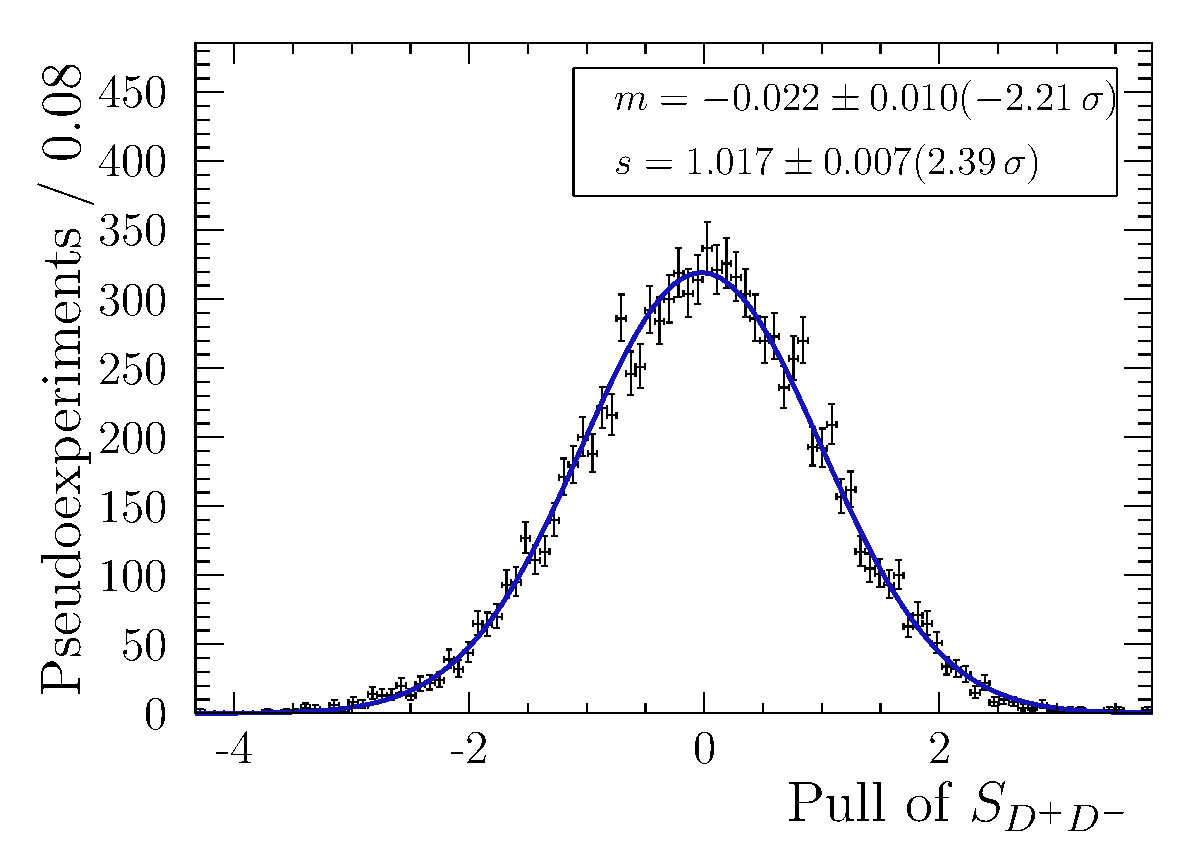
\includegraphics[width=0.49\textwidth]{07-B02DD/tikz/pdf/parSigTimeSin2b_pull_fitbias.pdf}
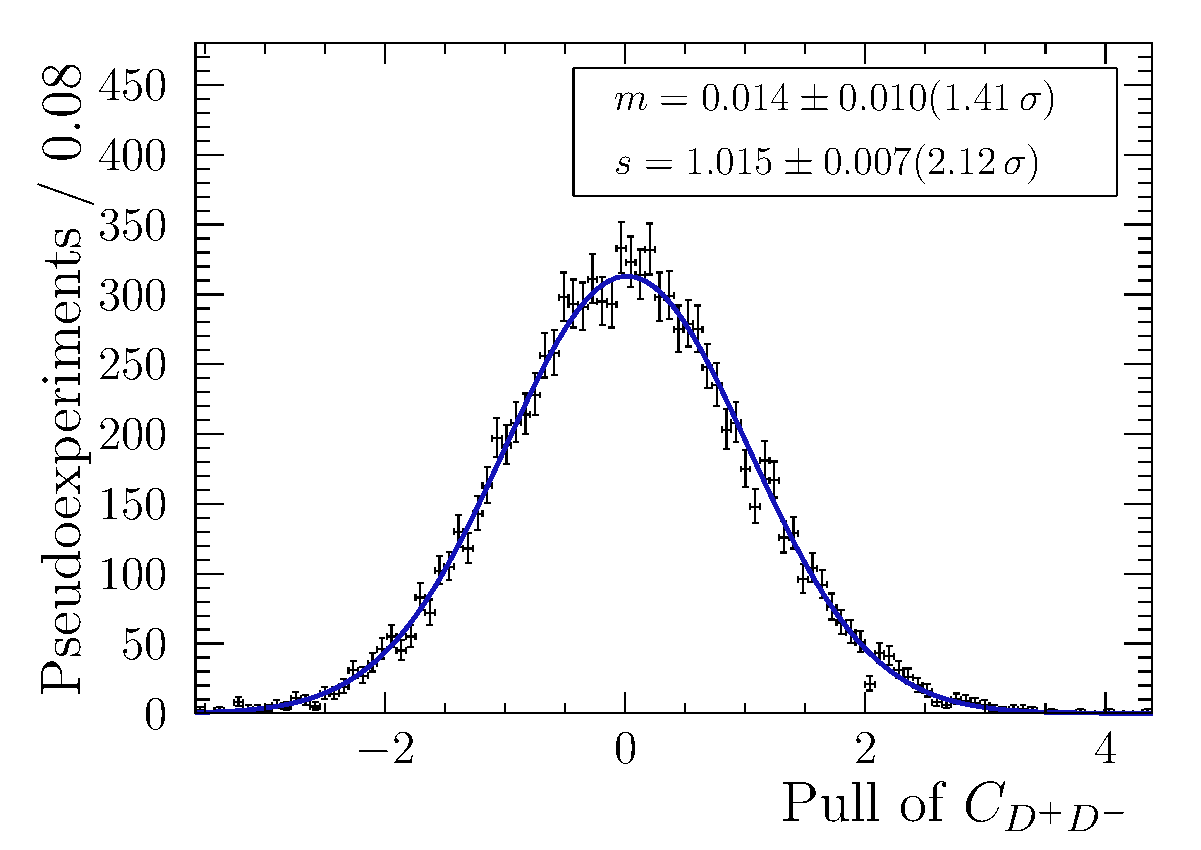
\includegraphics[width=0.49\textwidth]{07-B02DD/tikz/pdf/parSigTimeC_pull_fitbias.pdf}
\caption{Pull distributions of $\SDD$ and $\CDD$ for a study on the systematic
uncertainty due to the likelihood fitter.}
\label{fig:b02dd:systematics:fitbias:pulls}
\end{figure}
%
Multiplying it with the statistical uncertainty the systematic uncertainty is
calculated to be
\begin{align}
s_{\SDD}^{\textrm{fit}} = \num{0.004}\ , \qquad s_{\CDD}^{\textrm{fit}} = \num{0.0025}\ .
\end{align}
For all following studies of systematic uncertainties the residuals are
corrected for the decay time fit bias. Otherwise, even effects that are
actually not biasing would be misinterpreted due to the fit bias.

%============================================================================%
\subsection{Fit Model}
\label{sec:b02dd:systematics:fitmodel}
%!TEX root = ../main.tex

%----------------------------------------------------------------------------%
\subsubsection{Mass Model}
\label{sec:b02dd:systematics:massmodel}

Two different aspects of the mass model are studied regarding systematic
uncertainties: the impact of neglecting contributions and of mismodelling
components.

\paragraph{Neglected contributions}

If a neutral \piz or a photon is missed in the reconstruction the decay
\BToDstD, with \DstpToDpizero or \DstpToDgamma, can mimic the \BToDD decay. In
the rest frame of the \Dstarp resonance, the missing momentum of the \piz is
fixed, but it needs to be boosted when transferred into the rest frame of the
\PB meson. So, the reconstructed mass depends on the helicity angle of the
missing \piz. This leads to a double-horned structure approximately
\SI{140}{\MeVcc} below the nominal \PB mass (see Ref.~\cite{LHCb-ANA-2014-015}
for more details on the shape of this background). As the lower boundary on
the invariant $m_{\Dp\Dm}$ mass is set to \SI{5150}{\MeVcc} the \BdToDstD
contribution lies outside the mass range used for the fit. However, the
\BsToDstD contribution enters the fit region. But since the expected number of
\BsToDstD candidates is low, it is not included in the nominal mass model.
Another contribution that is neglected in the nominal mass fit model is
(partially) charmless background where at least one of the hadron triplets is
not originating from a \PD decay. The systematic uncertainty on the
determination of the \CP observables arising from neglecting these two
contributions is estimated using \num{1000} pseudoexperiments. Components for
\BsToDstD and for (partially) charmless background are included in the
generation but excluded from the fit procedure.

The shape of \BsToDstD is parametrised with two single Gaussian functions
centred around \SI{5150}{\MeVcc} and \SI{5200}{\MeVcc}. The (partially)
charmless background is modelled with a single Gaussian function. When
optimising the decay time significance cut it has been observed that the width
of the (partially) charmless background is approximately \SI{10}{\percent}
wider than the signal component. Therefore, a width of \SI{10}{\MeVcc} is
chosen. The mean is set to the same position as the \Bd signal. The \BsToDstD
component is generated without any tagging asymmetry, while for the (partially)
charmless background the worst case scenario of maximal \CP violation with the
opposite \CP eigenvalue ($S_f = \num{+1.0}$) is tested.

In studies of \BdToDstD decays~\cite{BToDstDthesis} a significant contribution
of \BsToDstD candidates is observed. The ratio between the two yields is
determined to be 1:20. Under the assumption that the efficiencies for \BToDD
and \BToDstD are the same the expected number of \BsToDstD candidates can be
calculated via
\begin{align}
	\text{N}_{\BsToDstD} = \frac{1}{20} \text{N}_{\BdToDD} \frac{\mathcal{B}(\BdToDstD) \mathcal{B}(\Dstarp \!\to \Dp (\piz || \gamma))}{\mathcal{B}(\BdToDD)} \,.
\end{align}
Using the world averages for the branching ratios~\cite{PDG2016} the number of
candidates to be generated in the pseudoexperiments is estimated to be
N(\BsToDstD) = \num{66\pm9}.

To determine how many (partially) charmless background candidates need to be
generated the $D$ mass window is widened to $\SI{\pm40}{\MeVcc}$ and the
nominal $D$ mass window of $\SI{\pm25}{\MeVcc}$ is vetoed for one or for both
$D$ candidates. Fits to the invariant $B$ mass without the $D$ mass constraint
are performed in the various scenarios. % yielding
% $\num{0.0\pm2.6}\,\mbox{\Bd\!\to\KpipiKpipi}$ candidates,
% $\num{0.0\pm9.2}\,\mbox{\Bd\!\to\KKpiKpipi}$ candidates,
% $\num{0.0\pm4.9}\,\mbox{\Bd\!\to\D(\Kpipi)\Kpipi}$ candidates,
% $\num{0.0\pm3.3}\,\mbox{\Bd\!\to\D(\KKpi)\Kpipi}$ candidates, and
% $\num{17.2\pm11.2}\,\mbox{\Bd\!\to\D(\Kpipi)\KKpi}$ candidates.
%
The fitted yields, which are constrained to positive values, are scaled to
account for the applied $D$ mass window. The total amount of residual
contamination ($\Bz\!\to\PD hhh$ or $\Bz\!\to hhhhhh$ decays) surviving the
\BdToDD selection is found to be $\num{28.7\pm19.5}$ candidates for the
$\KKpiKpipi$ final state and $\num{0.0\pm27.8}$ candidates for the
$\KpipiKpipi$ final state. For the pseudoexperiments the number of (partially)
charmless background is drawn from Gaussian distributions using these values
for mean and width. When the outcome is negative the procedure is repeated,
until a positive yield is drawn.

The systematic uncertainties on \SDD and \CDD are calculated as the product of
the bias on the mean parameter of the pull distributions and the statistical
uncertainty:
\begin{align*}
s_{\SDD}^{\text{mass,1}} = \num{0.05}\ , \qquad s_{\CDD}^{\text{mass,1}} = \num{0.013}\,.
\end{align*}

\paragraph{Mismodelling of mass components}

The BDT is trained with MC samples that are known to not perfectly model the
PID information. As a result the BDT classifier distributions of
background-subtracted data and MC show a quite big discrepancy. Some shape
parameters are estimated on MC samples and might be distorted by the data/MC
differences. Therefore, different alternative mass parametrisations are tested
against the nominal model: the component of the \BdToDD signal (and of the
\BsToDD background) is parametrised with a single Gaussian function; the
combinatorial background is described with a second order Chebyshev polynomial
of first kind; the tail parameters of \BToDsD are once extracted from the MC
sample without applying the BDT and once applying a tight cut on the BDT
classifier. The mass fit is performed with these new models, sWeights are
calculated for each approach, and the decay time fit is performed. The results
of the \CP observables are then compared with the nominal central values. The
largest deviations for \SDD and \CDD are
\begin{align*}
s_{\SDD}^{\text{mass,2}} = \num{0.004}\ , \qquad s_{\CDD}^{\text{mass,2}} = \num{0.006}\,.
\end{align*}

%----------------------------------------------------------------------------%
\subsubsection{Correlation between decay time and mistags}
\label{sec:b02dd:systematics:correlation_mistag_time}

The correlation between the decay time distribution and the per-event mistags
is studied by calculating the linear Pearson correlation coefficient
$\rho(\eta,t)$. The significance of the correlation value, \ie
\SI{95}{\percent} confidence level interval, is determined using the
bootstrapping method (\cref{sec:dataanalysis:bootstrapping}) with \num{10000}
repetitions. The correlation coefficients are found to be small. The profile
histogram of the OS tagging combination, which shows the average \etaos value
as a function of the decay time, is flat within statistics. For the SS tagging
combination the profile histogram slowly increases with decay time. This can
be confirmed by analysing the larger signal MC sample (see
\cref{fig:b02dd:systematics:correlation_mistag_time:etass_time_profile_MC}).
\begin{figure}[htb]
\centering
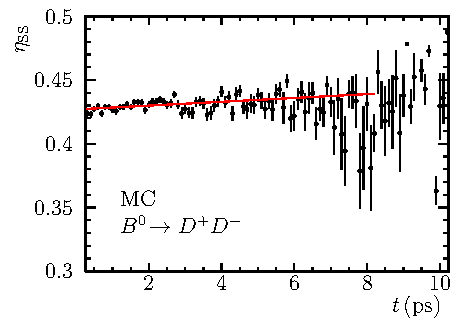
\includegraphics[width=0.6\textwidth]{07-B02DD/tikz/pdf/Profile_DecayTime_SS.pdf}
\caption{Profile histogram for the decay time dependence on $\etass$ for
signal MC. The black data points represent the mean value of $\etass$ and its
uncertainty for each bin in $t$. The red curve is the fitted linear function.}
\label{fig:b02dd:systematics:correlation_mistag_time:etass_time_profile_MC}
\end{figure}
Performing a $\chisq$ fit in the decay time range \SIrange{0.25}{8.25}{\ps}
with the linear function
\begin{align}
  \etass = a_{\etass,t} t + b_{\etass,t}
  \label{eq:tagging:correlation_mistag_time}
\end{align}
yields a slope of $a_{\etass,t} = \SI{1.50\pm0.27}{\invns}$. Although this is
a significant deviation from zero, the correlation is not taken into account in
the nominal fit model. Instead, a study on the systematic uncertainty from
neglecting this effect is performed. In \num{1000} pseudoexperiments the SS
mistag is generated using a Gaussian distribution whose mean is drawn from the
linear function defined in \cref{eq:tagging:correlation_mistag_time} thereby
introducing the correlation with the decay time. In the subsequent fit the
correlation is again ignored. This leads to systematic uncertainties of
\begin{align*}
s_{\SDD}^{\text{corr}} = \num{0.0007}\ , \qquad s_{\CDD}^{\text{corr}} = \num{0.007}\,.
\end{align*}

%----------------------------------------------------------------------------%
\subsubsection{Decay Time Resolution Model}
\label{sec:systematics:decaytimeresolution}

As calculated in \cref{sec:b02dd:decaytimefit:resolution} even an
underestimation of the decay time resolution by \SI{15}{\percent} has only a
minor effect on the resolution related dilution. Nevertheless, \num{1000}
pseudoexperiments are performed, in which the scale factors and the offset
parameters ($b_i$ and $c_i$ from \cref{tab:b02dd:decaytimefit:resolution}) are
enlarged by \SI{15}{\percent} in the generation and fixed to their nominal
values in the fit. Additionally, the mean parameter of the Gaussians is set to
the value obtained in the MC study for the generation and, like in the nominal
setup, fixed to zero in the fit. The systematic uncertainties are calculated
as the product of the biases on the mean parameter and the statistical
uncertainty to be
\begin{align*}
s_{\SDD}^{\text{res}} = \num{0.0020}\ , \qquad s_{\CDD}^{\text{res}} = \num{0.0023}\,.
\end{align*}

%----------------------------------------------------------------------------%
\subsubsection{Decay Time Acceptance Model}
\label{sec:systematics:decaytimeacceptance}

On signal MC the decay time acceptance is determined separately for the two
final states (see \cref{fig:b02dd:decaytimefit:acceptance_MC}). Small
differences are observed. As the low statistics in the \KKpiKpipi final state
on data does not allow for an individual spline model, a study is performed to
estimate a possible systematic uncertainty from neglecting this difference. In
\num{1000} pseudoexperiments the decay time distribution is generated using
the histograms of the true decay time acceptance from signal MC, split by
final state, and fitted with the spline acceptance as done in the nominal fit.
The use of the histograms with \num{100} bins should also cover uncertainties
from the choice of the number and position of the knots. The pull between the
fit results and the generation values is calculated. The systematic
uncertainty due to the decay time acceptance model is calculated as the
product of the shift in the pull distribution and the statistical uncertainty
of the nominal fit:
\begin{align*}
s_{\SDD}^{\textrm{acc}} = \num{0.007}\ , \qquad s_{\CDD}^{\textrm{acc}} = \num{0.0027}\,.
\end{align*}


%============================================================================%
\subsection{Further Studies}
\label{sec:b02dd:systematics:others}
%!TEX root = ../main.tex

%----------------------------------------------------------------------------%
\subsubsection[\texorpdfstring{$z$}{z}-scale]{\texorpdfstring{$\boldsymbol{z}$}{z}-scale}
\label{sec:b02dd:systematics:z_scale}

The decay times are determined by measuring the distance between PV and decay
vertex. So, any uncertainty on the positioning of detector elements
(especially the VELO modules) leads to biased decay times. Due to the high
boosting the main contribution to the flight distance is in $z$ direction. The
scale uncertainty in $z$ direction has been estimated to be
$\sigma_{z\text{-scale}} = \SI{0.022}{\percent}$~\cite{LHCb-ANA-2011-055}. The
influence on the measurement of the \CP observables is studied by performing
\num{1000} pseudoexperiments. For each pseudoexperiment a value for the uncertainty
on the $z$-scale is drawn from a Gaussian distribution around zero of width
$\sigma_{z\text{-scale}}$. The sum of \SI{50}{\fs} and the product of this
value with the decay time is used as width of the Gaussian function modelling
the decay time resolution in the generation. In the fit the width is set to
\SI{50}{\fs}. The product of the bias from the pull distributions of the
pseudoexperiments and the nominal statistical uncertainty is taken as
systematic uncertainty:
\begin{align*}
s_{\SDD}^{z\text{-scale}} = \num{0.0031}\ , \qquad s_{\CDD}^{z\text{-scale}} = \num{0.0028}\,.
\end{align*}

%----------------------------------------------------------------------------%
\subsubsection{Production Asymmetry}
\label{sec:b02dd:systematics:production_asymmetry}

The systematic uncertainty on the production asymmetry \prodasym{11} is
studied using \num{1000} pseudoexperiments. The nominal value is used in the
generation and the procedure described in Ref.~\cite{Karbach:1490463} is
applied in the fit: Before fitting the data sample the mean of the Gaussian
constraint for \prodasym{11} is shifted by one systematic uncertainty. The
resulting Gaussian distribution is used to draw a new value for the mean.
Then, the new Gaussian distribution is used to constrain \prodasym{11} in the
fit. Both shifts, upwards and downwards, are tested and the larger deviation
is taken as systematic uncertainty:
%
\begin{align*}
s_{\SDD}^{\prodasym{}} = \num{0.0015}\ , \qquad s_{\CDD}^{\prodasym{}} = \num{0.004}\,.
\end{align*}
%
For the production asymmetry difference $\Delta\prodasym{}$ the systematic
uncertainty is already included in the Gaussian constraint of the nominal fit.

%----------------------------------------------------------------------------%
\subsubsection{Decay Width Difference \texorpdfstring{\DGd}{Delta Gamma\_d}}
\label{sec:b02dd:systematics:deltagammad}

The decay width difference \DGd is expected to be very small and therefore
fixed to zero in the nominal fit. But experimentally it has a relatively large
uncertainty. This is taken into account by performing \num{1000}
pseudoexperiments where the current statistical precision $\sigma(\DGd) =
\SI{\pm0.007}{\invps}$~\cite{HFAG} is used in the generation of the data
samples while it is, like in the nominal model, neglected in the fit. The mean
parameters of the pull distributions are converted into systematic
uncertainties of
\begin{align*}
s_{\SDD}^{\DGd} = \num{0.014}\ , \qquad s_{\CDD}^{\DGd} = \num{0.0021}\,.
\end{align*}

%----------------------------------------------------------------------------%
\subsubsection{\texorpdfstring{$\Bz$}{B0} Mass Difference \texorpdfstring{\dmd}{Delta m\_d}}
\label{sec:b02dd:systematics:deltamd}

The systematic uncertainty on the world average of \dmd
($\SI{\pm0.002}{\hbar\invps}$~\cite{HFAG}) is not covered by the Gaussian constraint that
is used in the nominal fit. Instead, it is analysed using \num{1000}
pseudoexperiments. In the generation the nominal model is used. Before
performing the fit the mean of the Gaussian distribution (its width is the
statistical precision of the world average) is shifted by one systematic
uncertainty (once up and once down) and a new value is drawn from the
distribution. This new constraint is then used in the minimisation. Looking at
the resulting pull distributions systematic uncertainties of
\begin{align*}
s_{\SDD}^{\dmd} = \num{0.0025}\ , \qquad s_{\CDD}^{\dmd} = \num{0.006}\,,
\end{align*}
are assigned.


% \FloatBarrier
%============================================================================%
\subsection{Total Systematic Uncertainty}
\label{sec:b02dd:systematics:total}

The systematic uncertainties are summarised in
\cref{tab:b02dd:systematics:total}. The full systematic uncertainty is
calculated by summing the individual uncertainties in quadrature.
%
\begin{table}[!htb]
\caption{Systematic uncertainties on the $\CP$ observables $\SDD$ and $\CDD$.}
\label{tab:b02dd:systematics:total}
  \centering
    \begin{tabular}{lSS}
      \toprule
      Origin & {\param{\sigma}{}{$\SDD$}} & {\param{\sigma}{}{$\CDD$}}    \\
      \midrule
      Neglecting components in mass model     &  0.05    & 0.013  \\
      $\DGd$                                  &  0.014   & 0.0021 \\
      Decay time acceptance                   &  0.007   & 0.0027 \\
      Correlation between mass and decay time &  0.0007  & 0.007  \\
      Parametrisation of PDFs in mass model   &  0.004   & 0.006  \\
      $\dmd$                                  &  0.0025  & 0.006  \\
      Fit bias                                &  0.004   & 0.0025 \\
      Production asymmetry                    &  0.0015  & 0.004  \\
      $z$-scale                               &  0.0031  & 0.0028 \\
      Decay time resolution                   &  0.0020  & 0.0023 \\
      \midrule
      Sum                                     &  0.05    & 0.018  \\
      \bottomrule
    \end{tabular}
\end{table}

%!TEX root = ../main.tex

\chapter{Discussion}
\label{sec:discussion}

%!TEX root = ../main.tex

\section{Comparison with previous measurements of \texorpdfstring{$\sintwobetaoreff$}{sin2beta(eff)}}
\label{sec:discussion:sin2betahistory}

Measurements of \CP violation in \BdToJPsiKS decays have been performed since
the end of the nineties. The first results by OPAL~\cite{OPAL_sin2beta},
ALEPH~\cite{ALEPH_sin2beta} and CDF~\cite{CDF_sin2beta} had an uncertainty on
\sintwobeta no better than \num{\pm0.4}. One of the main purposes of the
$B$-factories was to improve the precision, which succeeded with results of
$\SJpsiKS = \num[parse-numbers=false]{0.657\pm0.036\pm0.012}$ by
\babar~\cite{BaBar_sin2beta} and $\SJpsiKS =
\num[parse-numbers=false]{0.670\pm0.029\pm0.013}$ by
\belle~\cite{Belle_sin2beta}. Averaging the results of the $B$-factories and
combining them with measurements in various other charmonium modes leads to an
average of \sintwobeta = \num{0.679\pm0.020}~\cite{HFAG}. The measurement
presented in this thesis, using data corresponding to an integrated luminosity
of \SI{3}{\invfb} collected with the \lhcb experiment, further improves on
this yielding an updated world average of \sintwobeta =
\num{0.691\pm0.017}~\cite{HFAG}. There is also the possibility to constrain
$\beta$ from a global fit to the CKM triangle. When not using the inputs from
the direct measurements described above ($\beta =
\SI{21.85\pm0.7}{\degrees}$), a value of $\beta = (24.3
^{+1.3}_{-1.4})\,\degrees$~\cite{CKMfitter} is found. This shows that the
value found by \lhcb improves the compatibility between the direct and the
indirect measurements by shifting \sintwobeta slightly upwards.

While for \BdToJPsiKS decays mainly the value of \SJpsiKS is interesting, as
it is expected to correspond to \sintwobeta with only small corrections, the
same does not apply for the measurement of \CP violation using \BdToDD decays.
Both observables, \SDD and \CDD, have to be considered simultaneously for a
proper interpretation of the results. In \cref{fig:discussion:b2ddcomparison}
the latest results from \babar, \belle, and \lhcb, as well as the average of
these three are plotted in the two-dimensional plane of \CDD versus \SDD.
\begin{figure}[htb]
\centering
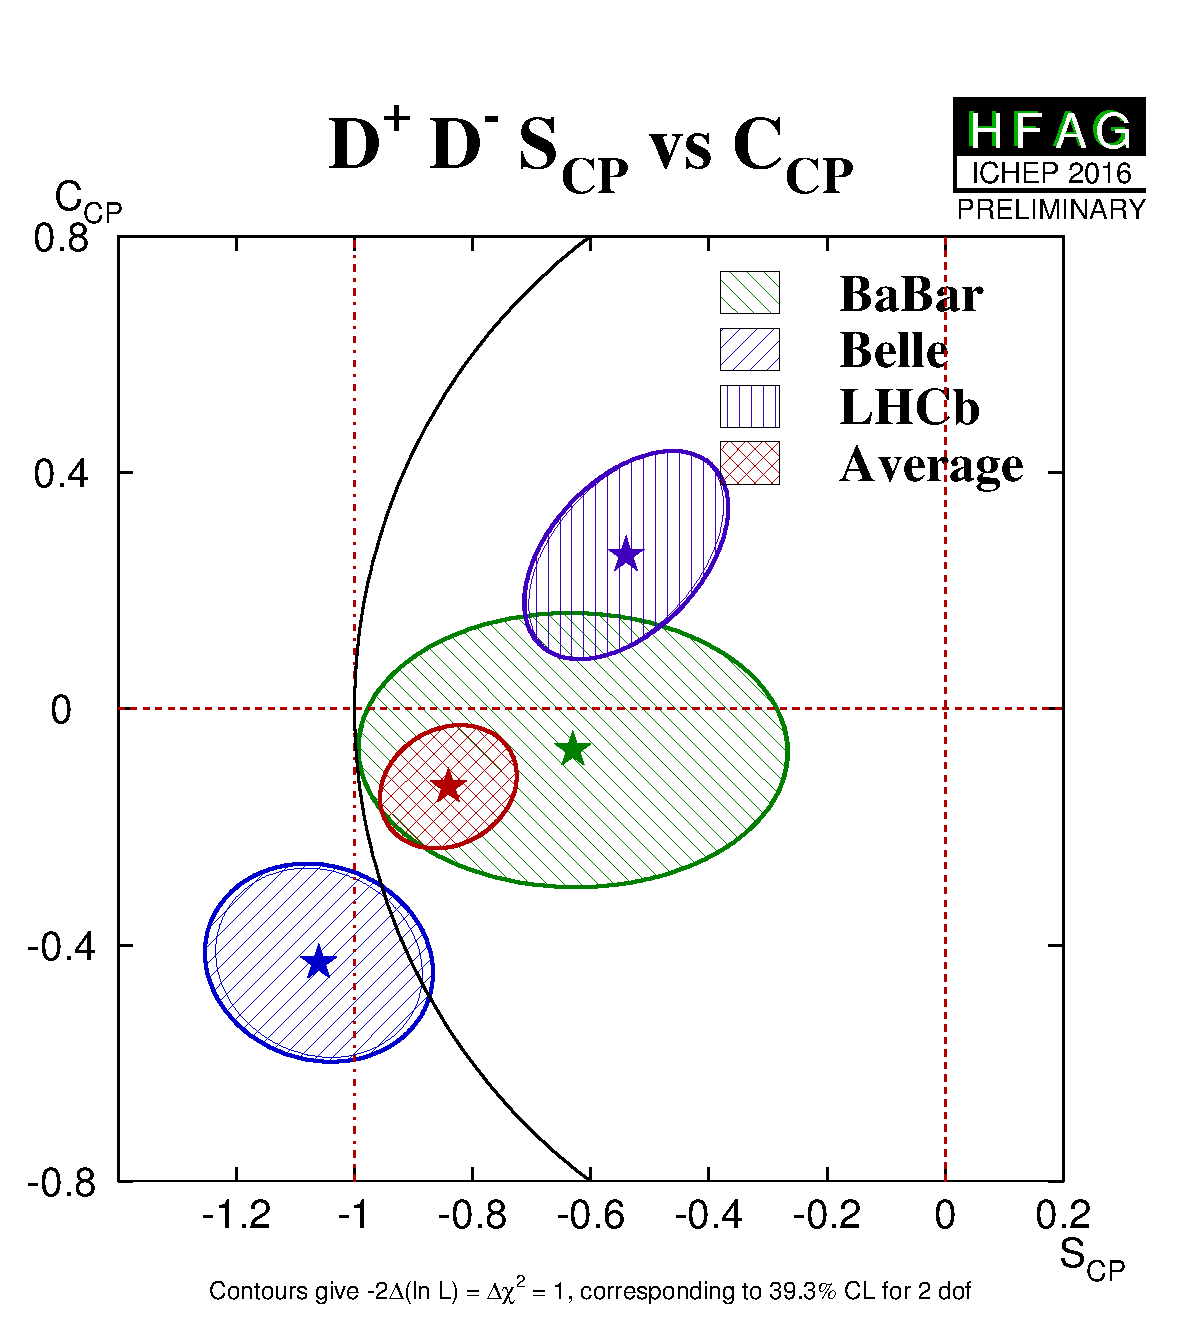
\includegraphics[width=0.5\textwidth]{08-Discussion/figs/D+D-S_CPvsC_CP.pdf}
\caption{Comparison of \CP observables from \mbox{\BdToDD} decays in (\SDD,
\CDD) plane~\cite{HFAG}. The contours give $-2\Delta(\ln L) = \Delta\chisq =
1$, thereby corresponding to a coverage of \SI{39.3}{\percent} for 2 degrees
of freedom.}
\label{fig:discussion:b2ddcomparison}
\end{figure}
Looking at the uncertainty ellipses it is apparent that the precision of \lhcb
matches the one of \belle, while being significantly better than the one of
\babar. The orientation of the ellipses shows that in the measurements of the
$B$-factories the two \CP observables are determined almost uncorrelated. For
a comparison of the central values it is useful to take into account the arc
defined by the condition $\SDD^2+\CDD^2=1$. It represents the extreme case of
$\lambda_{\Dp\Dm}$ being purely imaginary and delimits the physically allowed
region. The result by \belle~\cite{Rohrken:2012ta} of \SDD = \num{-1.06} and
\CDD = \num{-0.43} lies outside, while the results of
\babar~\cite{Aubert:2008ah}, which are \SDD = \num{-0.63} and \CDD =
\num{-0.07}, as well as the result of \lhcb (see
\cref{eq:b02dd:decaytimefit:cpresults}) are inside.


\section{Comparison between \texorpdfstring{$\CP$}{CP} violation in
\texorpdfstring{\mbox{$\BdToJPsiKS$}}{Bd2JPsiKS} and in
\texorpdfstring{\mbox{$\BdToDD$}}{Bd2DD} decays}
\label{sec:discussion:JpsiKS_DD_comparison}

Measurements in decays with \bToccbars transitions have established the
presence of \CP violation in the system of neutral $B$ mesons with very high
precision. Comparing the plots of the decay-time-dependent signal yield
asymmetry for \BdToJPsiKS and \BdToDD decays (see
\cref{fig:discussion:asymmetry}), the difference in sensitivity becomes
apparent.
\begin{figure}[hbt]
\centering
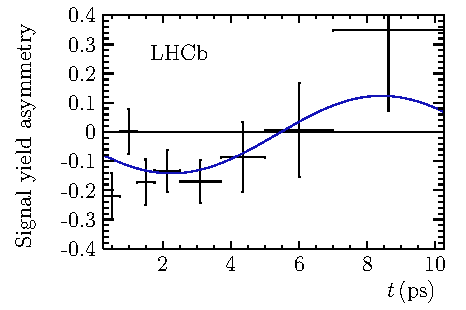
\includegraphics[width=0.49\textwidth]{08-Discussion/tikz/pdf/Asymmetry_B2DD.pdf}
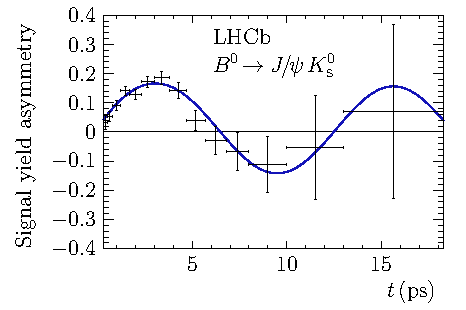
\includegraphics[width=0.49\textwidth]{08-Discussion/tikz/pdf/Asymmetry_B2JPsiKS.pdf}
\caption{Signal yield asymmetry from \BdToDD decays~\cite{LHCb-PAPER-2016-037} (left)
and \BdToJPsiKS decays~\cite{LHCb-PAPER-2015-004} (right).}
\label{fig:discussion:asymmetry}
\end{figure}
However, the main motivation for the measurement of \CP violation in \BdToDD
decays, presented in this thesis, is not to achieve the single best
measurement of \CP violation. In fact, given the uncertainties the
conservation of \CP symmetry can be excluded by only \num{4.0} standard
deviations with this measurement. Instead, the phase shift $\Delta\phi$ can be
obtained, which is caused by higher-order Standard Model contributions and
complicates the determination of $\beta$ and $\betas$ similarly (see
\cref{sec:cpviolation:btoccbard}). The fit results of $\SDD$ and $\CDD$ (see
\cref{eq:b02dd:decaytimefit:cpresults}) correspond to
\begin{align*}
  \sin(\phid + \Delta \phi) = \frac{-\SDD}{\sqrt{1 - \CDD^2}} = 0.56\,\pm\,^{0.16}_{0.17}\,,
\end{align*}
where the statistical uncertainty is estimated by generating three million
sets of \SDD and \CDD using a two-dimensional Gaussian distribution including
their correlation, calculating $\sin(\phid + \Delta \phi)$ for each of them,
and then taking the two-sided \SI{68}{\percent} confidence intervals. This
result can be combined with the corresponding value from \BdToJPsiKS to
extract the phase shift $\Delta \phi$. The calculation yields $\Delta \phi =
-0.16\,^{+0.19}_{-0.21}$\,\si{\radian}, which is significantly more precise
than the previous measurement using the results by the $B$-factories of
$\Delta \phi = (30\,^{+23}_{-30})\si{\degrees} =
0.52\,^{+0.40}_{-0.56}$~\cite{Bel:2015wha}, and thus represents the world's
most precise determination of this quantity. Moreover, the size of the
higher-order corrections is reduced by more than a factor of three and is
compatible with zero.

%!TEX root = ../main.tex

\chapter{Conclusion}
\label{sec:conclusion}

Since the discovery of \CP violation in 1964 by Christenson, Cronin, Fitch and
Turlay~\cite{CPV_discovery} there have been many experiments searching for \CP
violation, first in the sector of neutral $K$ mesons but later on also for
neutral $B$ mesons. The most significant indication of \CP violation for \Bz
mesons is found by the determination of \sintwobeta using \BdToJPsiKS decays.
But although \lhcb is not the first experiment, even not at a hadron collider,
to measure \CP violation it plays an important role in the further exploration
of the quark-mixing sector.

The measurement of \CP violation in \BdToJPsiKS
decays~\cite{LHCb-PAPER-2015-004} using proton-proton collision data
corresponding to an integrated luminosity of \SI{3}{\invfb}, which is
presented in this thesis, yields
\begin{align*}
  \SJpsiKS &=  \phantom{-}0.731 \, \pm 0.035 \, \text{(stat)} \pm 0.020 \, \text{(syst)}\,, \\
  \CJpsiKS &=  			- 0.038 \, \pm 0.032 \, \text{(stat)} \pm 0.005 \, \text{(syst)}\,,
\end{align*}
which is the most precise determination of these \CP observables at a hadron
collider to date and is almost as precise as the previous measurements by
\babar~\cite{BaBar_sin2beta} and \belle~\cite{Belle_sin2beta}. The central
values are compatible with the world averages and with the Standard Model
expectations. Thus, it serves as a benchmark measurement showing the
capability of \lhcb to perform flavour-tagged precision measurements of \CP
violation. The experimental difficulties, \eg decay time resolution,
production asymmetries and asymmetries induced by the flavour tagging, are
well under control as the result is statistically limited. The largest
systematic uncertainty on \SJpsiKS is introduced by a possible tagging
asymmetry of the background, which is not accounted for in the likelihood fit
(see \cref{sec:bd2jpsiks:systematics}). With an increased statistics this
effect can probably be analysed, controlled and suppressed better.
Furthermore, in the meantime new same-side flavour-tagging algorithms have
been developed~\cite{LHCb-PAPER-2016-039}, which are used for the first time
in the measurement of \CP violation in \BdToDD
decays~\cite{LHCb-PAPER-2016-037} yielding
\begin{align*}
  \SDD &=  -0.54 \, ^{+0.17}_{-0.16} \, \text{(stat)} \pm 0.05 \, \text{(syst)}\,, \\
  \CDD &=  \phantom{-}0.26 \, ^{+0.18}_{-0.17} \, \text{(stat)} \pm 0.02 \, \text{(syst)}\,.
\end{align*}
If the flavour-tagging performance was the same as in the \BdToJPsiKS
analysis, the 70 times lower number of available untagged signal candidates
(\num{114000} \BdToJPsiKS decays vs. \num{1610} \BdToDD decays) would only
allow a sensitivity of \num{\pm0.29} and \num{\pm0.27} for \SDD and
\CDD, respectively. However, the kinematic properties of the selected \BdToDD
candidates lead to a significantly higher tagging power and on top of that the
usage of the improved flavour-tagging algorithms increases the tagging power
by another \SI{20}{\percent}. The latter improvement can probably be exploited
in future measurements of \sintwobeta with \BdToJPsiKS decays. The value of
\effeff = \SI{8.1}{\percent} for the \BdToDD sample is the highest tagging
power to date in a tagged \CP violation measurement at \lhcb.

The main achievement by the measurement of \CP violation in \BdToDD decays is
to constrain the contribution of higher-order Standard Model corrections to be
small. The result of
\begin{align*}
	\Delta \phi = -0.16\,^{+0.19}_{-0.21}\,\si{\radian}
\end{align*}
can be transferred to the measurement of \CP violation in \BsToDsDs
decays~\cite{LHCb-PAPER-2014-051}, where \phis, the mixing phase of the \Bs
meson sector, can be determined, but only in a sum with this phase shift.

The analysis of \BdToDD decays is only the starting point for similar
measurements in other \allBToDD decay modes. First studies using \BdToDstD
decays have already been performed~\cite{BToDstDthesis}. Recent calculations
taking into account the flavour-tagging performance seen in \BdToDD and the
increase in statistics when adding data from Run~II indicate that the
sensitivity of \babar~\cite{Aubert:2008ah} and \belle~\cite{Rohrken:2012ta}
could be reached and even be topped.

The question is, what comes next? More and more data is collected at the \lhc
during Run~II and due to the higher centre-of-mass energy of currently
\SI{13}{\TeV} the \bbbar cross section, which roughly scales linearly with the
centre-of-mass energy, is even increased with respect to the proton-proton
collisions recorded during Run~I. In principle, the instantaneous luminosity
is another adjusting screw to further increase the data samples, though it is
already higher than the design value originally planned in the proposal for
the detector~\cite{LHCb-Technical-Proposal}. However, a key to significant
improvements, especially for decays with hadronic final states but also for
measurements of charmonium, is the performance of the trigger system. After
the upgrade in 2018--2020 it is planned to read out the full detector at
\SI{30}{\mega\hertz}~\cite{LHCb-TDR-016}. Right now, the signal efficiency of
the hardware trigger is not higher than \SI{50}{\percent}. Therefore, a large
potential for improvements exists. Another important aspect of tagged \CP
violation measurements is the performance of the flavour-tagging algorithms.
The higher the occupancy in the detector the more difficult it is to find the
appropriate tagging particle. There are ideas, at least for Run~II, how to
accommodate for this and the higher centre-of-mass energy helps in regaining
the flavour-tagging performance of Run~I.

Only the combination of all these efforts to increase the available amount of
data to be analysed might result in the observation of deviations from the
Standard Model expectations and thus an indirect hint for new physics. It's
not really a question of if new physics is needed but rather of how it looks
like. No dark matter candidate has been found so far. The origin of the
baryonic universe with the absence of antimatter can not be explained by the
amount of \CP violation incorporated in the SM.

\todo{Belle 2 and other future experiments like ILC?}


%\addcontentsline{toc}{chapter}{Appendices}
%!TEX root = ../main.tex

\clearpage
\appendix

\chapter{Appendices}

\section{First appendix}

\clearpage
\addcontentsline{toc}{chapter}{Bibliography}
\setboolean{inbibliography}{true}
\bibliographystyle{LHCb}
\bibliography{99-References/bibliography,99-References/LHCb-PAPER,99-References/LHCb-CONF,99-References/LHCb-DP,99-References/LHCb-TDR,99-References/LHCb-ANA,99-References/LHCb-THESIS,99-References/external}

%%%%%%%%%%%%%%%%%%%%%%%%%
%%% Acknowledgmenets %%%%
%%%%%%%%%%%%%%%%%%%%%%%%%
\addcontentsline{toc}{chapter}{Acknowledgements}
%!TEX root = ../main.tex

\chapter*{Acknowledgements}

\selectlanguage{ngerman}
Zunächst möchte ich mich bei Herrn Spaan bedanken. Seitdem ich im Oktober 2011
an Ihren Lehrstuhl gekommen bin, um erst meine Masterarbeit und nun diese
Doktorarbeit zu schreiben, waren Sie immer mit Rat und Tat für mich da.
Zusätzlich haben Sie uns immer wieder mit interessanten Anekdoten unterhalten.

Mein Dank gilt auch Professor Kröninger, der sich bereit erklärt hat, als
Zweitgutachter für meine Dissertation zu fungieren.

In den ersten zwei Jahren meiner Dissertation habe ich gemeinsam mit
Christophe an der Messung von CP Verletzung in \BdToJPsiKS Zerfällen
gearbeitet. Wir haben uns gegenseitig unterstützt, und so nicht nur eine
gelungene Analyse abgeliefert, sondern auch jeweils Dissertationsschriften
verfassen können. Danke schön.

\selectlanguage{english}
High energy physics is often a complex field of study, where progress is
impossible without collaborative work. Thanks to Paul, Nicoletta and Marta for
working with me on the \BdToDD analysis, especially for performing and
providing the flavour-tagging calibration.

\selectlanguage{ngerman}
Ich möchte mich auch ganz herzlich bei meinen Bürokollegen Alex, Margarete und
insbesondere Uli bedanken. Es war immer eine wunderbare Arbeitsatmosphäre, in
der ich mich wohl gefühlt habe. Probleme wurden untereinander diskutiert und
auch für Gespräche außerhalb des Unialltags war immer Zeit.

Weiterer Dank gebührt Julian für gute Ratschläge, für das Teilen von
Erfahrungen, produktive Diskussionen und allgemein Hilfe bei vielen Passagen,
die Eingang in diese Arbeit gefunden haben.

Wenn man zu lange an einem Dokument wie dieser Dissertation schreibt, bemerkt
man oftmals gar nicht, dass Bezüge fehlen oder Sachverhalte ungenügend erklärt
worden sind. Deshalb bin ich Timon, Moritz, Vanessa und Alex sehr dankbar
dafür, sich die Zeit genommen und Teile meiner Arbeit Korrektur gelesen zu
haben.

Plots problemlos ansprechend aussehen zu lassen, komplexe Systematikstudien
mit wenigen Zeilen Code erstellen und auswerten zu können, sowie etliche
nützliche Funktionen zur Verfügung zu haben, ist ein Luxus, an den man sich
all zu schnell gewöhnt, obwohl eine Menge Arbeit dahinter gesteckt hat. Vielen
Dank, Florian, dass du das DooSoftware-Framework erstellt hast.

Meine Begeisterung für die Physik wurde in der Oberstufe durch den leider viel
zu früh verstorbenen Herrn Bär, meinen Physiklehrer im Leistungskurs, geweckt.
Auch wenn Sie das nicht lesen können, vielen Dank, ohne Sie wäre ich wohl
nicht hier gelandet.
\newpage

%%%%%%%%%%%%%%%%%%%%%%%%%
%%%%%% Erklärung %%%%%%%%
%%%%%%%%%%%%%%%%%%%%%%%%%

\ifthenelse{\boolean{wordcount}}{
}
{%!TEX root = ../main.tex

\thispagestyle{empty}
\begin{center}
\section*{Eidesstattliche Versicherung}
\end{center}
\vspace*{1cm}
Ich versichere hiermit an Eides statt, dass ich die vorliegende Dissertation mit dem Titel ''{Measurements of \sintwobeta using charmonium and open-charm decays at \lhcb}'' selbstständig und ohne unzul\"assige fremde Hilfe erbracht habe. Ich habe keine anderen als die angegebenen
Quellen und Hilfsmittel benutzt sowie w\"ortliche und sinngem\"a\ss e Zitate kenntlich gemacht.
Die Arbeit hat in gleicher oder \"ahnlicher Form noch keiner Pr\"ufungsbeh\"orde vorgelegen.
\vspace*{1cm}
\ \\
\line(1,0){150} \hfill \line(1,0){150}\\
Ort, Datum \hfill Unterschrift \hspace*{3cm}
\vspace*{1.4cm}

\subsection*{Belehrung}
Wer vors\"atzlich gegen eine die T\"auschung \"uber Pr\"ufungsleistungen betreffende Regelung einer Hochschulpr\"ufungsordnung
verst\"o\ss t handelt ordnungswidrig. Die Ordnungswidrigkeit kann mit einer Geldbu\ss e von bis zu \SI{50000}{\EUR} geahndet werden. Zust\"andige Verwaltungsbeh\"orde f\"ur die Verfolgung und Ahndung von Ordnungswidrigkeiten ist
der Kanzler/die Kanzlerin der Technischen Universit\"at Dortmund. Im Falle eines mehrfachen oder sonstigen schwerwiegenden T\"auschungsversuches kann der Pr\"ufling zudem exmatrikuliert werden (\S\ 63 Abs. 5 Hochschulgesetz).\\
\ \\
Die Abgabe einer falschen Versicherung an Eides statt wird mit Freiheitsstrafe bis zu 3 Jahren oder mit Geldstrafe bestraft.\\
\ \\
Die Technische Universit\"at Dortmund wird ggf. elektronische Vergleichswerkzeuge (wie z.B. die Software ''turnitin'') zur \"Uberpr\"ufung von Ordnungswidrigkeiten in Pr\"ufungsverfahren nutzen.\\
\ \\
Die oben stehende Belehrung habe ich zur Kenntnis genommen.
\vspace*{1cm}
\ \\
\ \\
\line(1,0){150} \hfill \line(1,0){150}\\
Ort, Datum \hfill Unterschrift \hspace*{3cm}
\vspace*{\fill}}

\end{document}
